\chapter{p4 = 41 (447 graphs)}
\newpage\begin{figure}
  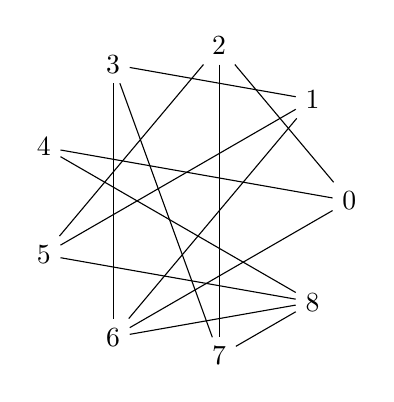
\begin{tikzpicture}
      \draw
        (0.0:2) node (0){0}
        (40.0:2) node (1){1}
        (80.0:2) node (2){2}
        (120.0:2) node (3){3}
        (160.0:2) node (4){4}
        (200.0:2) node (5){5}
        (240.0:2) node (6){6}
        (280.0:2) node (7){7}
        (320.0:2) node (8){8};
      \begin{scope}[-]
        \draw (0) to (2);
        \draw (0) to (4);
        \draw (0) to (6);
        \draw (1) to (3);
        \draw (1) to (5);
        \draw (1) to (6);
        \draw (2) to (5);
        \draw (2) to (7);
        \draw (3) to (6);
        \draw (3) to (7);
        \draw (4) to (8);
        \draw (5) to (8);
        \draw (6) to (8);
        \draw (7) to (8);
      \end{scope}
    \end{tikzpicture}
\end{figure}
\begin{itemize}
\item signature: 010101000101100001010001100001001011
\item g: Graph with 9 nodes and 14 edges
\item order: 9
\item size: 14
\item max degree: 4
\item degrees: 2,3,3,3,3,3,3,4,4
\item is tree: 0
\item is bipartite: 0
\item has bridge: 0
\item is chordal: 0
\item is complete: 0
\item min cycle basis weight: 24
\item min cycle basis size: 6
\item diameter: 3
\item radius: 2
\item is eulerian: 0
\item is planar: 0
\item number of faces: 7
\item is regular: 0
\item p3: 28
\item p4: 41
\item property hash: 7f80ce546656c11e388dfd0e80f67dd82dd3dee3bdbe5017d2e613b8ec34a3b1
\end{itemize}
\newpage
\begin{figure}
  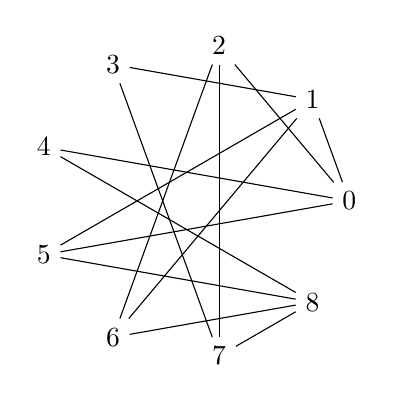
\begin{tikzpicture}
      \draw
        (0.0:2) node (0){0}
        (40.0:2) node (1){1}
        (80.0:2) node (2){2}
        (120.0:2) node (3){3}
        (160.0:2) node (4){4}
        (200.0:2) node (5){5}
        (240.0:2) node (6){6}
        (280.0:2) node (7){7}
        (320.0:2) node (8){8};
      \begin{scope}[-]
        \draw (0) to (1);
        \draw (0) to (2);
        \draw (0) to (4);
        \draw (0) to (5);
        \draw (1) to (3);
        \draw (1) to (5);
        \draw (1) to (6);
        \draw (2) to (6);
        \draw (2) to (7);
        \draw (3) to (7);
        \draw (4) to (8);
        \draw (5) to (8);
        \draw (6) to (8);
        \draw (7) to (8);
      \end{scope}
    \end{tikzpicture}
\end{figure}
\begin{itemize}
\item signature: 110110000101100000110000100001001011
\item g: Graph with 9 nodes and 14 edges
\item order: 9
\item size: 14
\item max degree: 4
\item degrees: 2,2,3,3,3,3,4,4,4
\item is tree: 0
\item is bipartite: 0
\item has bridge: 0
\item is chordal: 0
\item is complete: 0
\item min cycle basis weight: 24
\item min cycle basis size: 6
\item diameter: 3
\item radius: 2
\item is eulerian: 0
\item is planar: 0
\item number of faces: 7
\item is regular: 0
\item p3: 29
\item p4: 41
\item property hash: 18f25428d2987d42e565b20ca1d93e6287d2b8226802b1d717bcde2d1f05b0ab
\end{itemize}
\newpage
\begin{figure}
  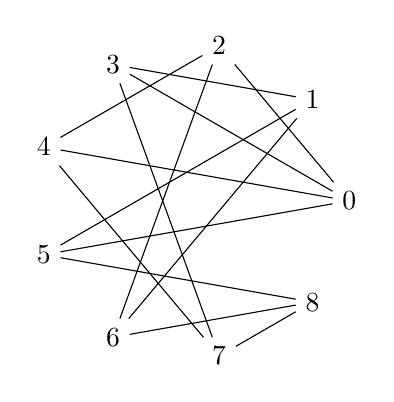
\begin{tikzpicture}
      \draw
        (0.0:2) node (0){0}
        (40.0:2) node (1){1}
        (80.0:2) node (2){2}
        (120.0:2) node (3){3}
        (160.0:2) node (4){4}
        (200.0:2) node (5){5}
        (240.0:2) node (6){6}
        (280.0:2) node (7){7}
        (320.0:2) node (8){8};
      \begin{scope}[-]
        \draw (0) to (2);
        \draw (0) to (3);
        \draw (0) to (4);
        \draw (0) to (5);
        \draw (1) to (3);
        \draw (1) to (5);
        \draw (1) to (6);
        \draw (2) to (4);
        \draw (2) to (6);
        \draw (3) to (7);
        \draw (4) to (7);
        \draw (5) to (8);
        \draw (6) to (8);
        \draw (7) to (8);
      \end{scope}
    \end{tikzpicture}
\end{figure}
\begin{itemize}
\item signature: 011110000101100010100000100010001011
\item g: Graph with 9 nodes and 14 edges
\item order: 9
\item size: 14
\item max degree: 4
\item degrees: 3,3,3,3,3,3,3,3,4
\item is tree: 0
\item is bipartite: 0
\item has bridge: 0
\item is chordal: 0
\item is complete: 0
\item min cycle basis weight: 25
\item min cycle basis size: 6
\item diameter: 3
\item radius: 2
\item is eulerian: 0
\item is planar: 0
\item number of faces: 7
\item is regular: 0
\item p3: 27
\item p4: 41
\item property hash: 301a7e490738eb7d3838f0535cc74fc02b59b981f4b137de3ebd096916f7cf14
\end{itemize}
\newpage
\begin{figure}
  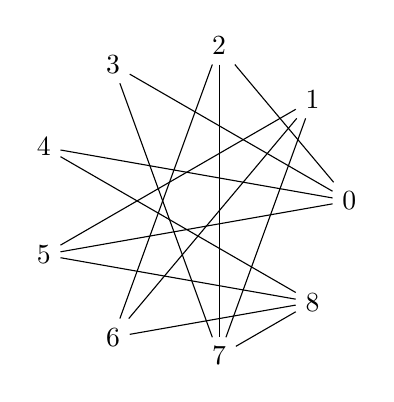
\begin{tikzpicture}
      \draw
        (0.0:2) node (0){0}
        (40.0:2) node (1){1}
        (80.0:2) node (2){2}
        (120.0:2) node (3){3}
        (160.0:2) node (4){4}
        (200.0:2) node (5){5}
        (240.0:2) node (6){6}
        (280.0:2) node (7){7}
        (320.0:2) node (8){8};
      \begin{scope}[-]
        \draw (0) to (2);
        \draw (0) to (3);
        \draw (0) to (4);
        \draw (0) to (5);
        \draw (1) to (5);
        \draw (1) to (6);
        \draw (1) to (7);
        \draw (2) to (6);
        \draw (2) to (7);
        \draw (3) to (7);
        \draw (4) to (8);
        \draw (5) to (8);
        \draw (6) to (8);
        \draw (7) to (8);
      \end{scope}
    \end{tikzpicture}
\end{figure}
\begin{itemize}
\item signature: 011110000001110000110000100001001011
\item g: Graph with 9 nodes and 14 edges
\item order: 9
\item size: 14
\item max degree: 4
\item degrees: 2,2,3,3,3,3,4,4,4
\item is tree: 0
\item is bipartite: 0
\item has bridge: 0
\item is chordal: 0
\item is complete: 0
\item min cycle basis weight: 25
\item min cycle basis size: 6
\item diameter: 3
\item radius: 2
\item is eulerian: 0
\item is planar: 0
\item number of faces: 7
\item is regular: 0
\item p3: 32
\item p4: 41
\item property hash: 28a8911d5e1964a17479dba6ba6fa3346ba8a1e99b7290c465a3a0a08ac00601
\end{itemize}
\newpage
\begin{figure}
  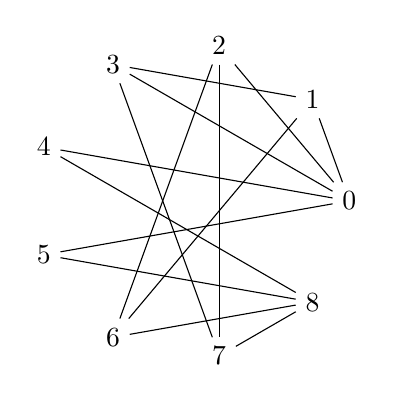
\begin{tikzpicture}
      \draw
        (0.0:2) node (0){0}
        (40.0:2) node (1){1}
        (80.0:2) node (2){2}
        (120.0:2) node (3){3}
        (160.0:2) node (4){4}
        (200.0:2) node (5){5}
        (240.0:2) node (6){6}
        (280.0:2) node (7){7}
        (320.0:2) node (8){8};
      \begin{scope}[-]
        \draw (0) to (1);
        \draw (0) to (2);
        \draw (0) to (3);
        \draw (0) to (4);
        \draw (0) to (5);
        \draw (1) to (3);
        \draw (1) to (6);
        \draw (2) to (6);
        \draw (2) to (7);
        \draw (3) to (7);
        \draw (4) to (8);
        \draw (5) to (8);
        \draw (6) to (8);
        \draw (7) to (8);
      \end{scope}
    \end{tikzpicture}
\end{figure}
\begin{itemize}
\item signature: 111110000100100000110000100001001011
\item g: Graph with 9 nodes and 14 edges
\item order: 9
\item size: 14
\item max degree: 5
\item degrees: 2,2,3,3,3,3,3,4,5
\item is tree: 0
\item is bipartite: 0
\item has bridge: 0
\item is chordal: 0
\item is complete: 0
\item min cycle basis weight: 24
\item min cycle basis size: 6
\item diameter: 2
\item radius: 2
\item is eulerian: 0
\item is planar: 0
\item number of faces: 7
\item is regular: 0
\item p3: 30
\item p4: 41
\item property hash: 82f35c16b10349c814ef4dd8dd738b69662f48541aa819ee203eaf1f2d1836c2
\end{itemize}
\newpage
\begin{figure}
  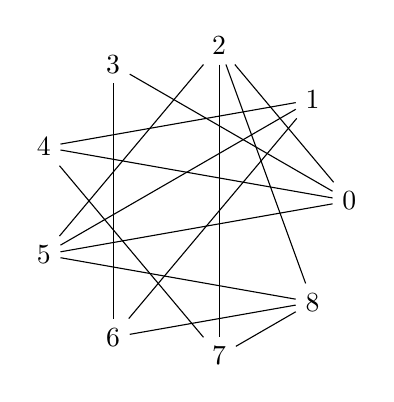
\begin{tikzpicture}
      \draw
        (0.0:2) node (0){0}
        (40.0:2) node (1){1}
        (80.0:2) node (2){2}
        (120.0:2) node (3){3}
        (160.0:2) node (4){4}
        (200.0:2) node (5){5}
        (240.0:2) node (6){6}
        (280.0:2) node (7){7}
        (320.0:2) node (8){8};
      \begin{scope}[-]
        \draw (0) to (2);
        \draw (0) to (3);
        \draw (0) to (4);
        \draw (0) to (5);
        \draw (1) to (4);
        \draw (1) to (5);
        \draw (1) to (6);
        \draw (2) to (5);
        \draw (2) to (7);
        \draw (2) to (8);
        \draw (3) to (6);
        \draw (4) to (7);
        \draw (5) to (8);
        \draw (6) to (8);
        \draw (7) to (8);
      \end{scope}
    \end{tikzpicture}
\end{figure}
\begin{itemize}
\item signature: 011110000011100001011001000010001011
\item g: Graph with 9 nodes and 15 edges
\item order: 9
\item size: 15
\item max degree: 4
\item degrees: 2,3,3,3,3,4,4,4,4
\item is tree: 0
\item is bipartite: 0
\item has bridge: 0
\item is chordal: 0
\item is complete: 0
\item min cycle basis weight: 26
\item min cycle basis size: 7
\item diameter: 3
\item radius: 2
\item is eulerian: 0
\item is planar: 0
\item number of faces: 8
\item is regular: 0
\item p3: 28
\item p4: 41
\item property hash: f86bee84b98cd980e9df1c117eba4f9a0261699db3d6459e6e2561116d18d07d
\end{itemize}
\newpage
\begin{figure}
  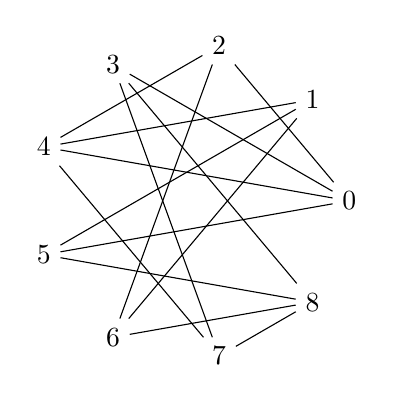
\begin{tikzpicture}
      \draw
        (0.0:2) node (0){0}
        (40.0:2) node (1){1}
        (80.0:2) node (2){2}
        (120.0:2) node (3){3}
        (160.0:2) node (4){4}
        (200.0:2) node (5){5}
        (240.0:2) node (6){6}
        (280.0:2) node (7){7}
        (320.0:2) node (8){8};
      \begin{scope}[-]
        \draw (0) to (2);
        \draw (0) to (3);
        \draw (0) to (4);
        \draw (0) to (5);
        \draw (1) to (4);
        \draw (1) to (5);
        \draw (1) to (6);
        \draw (2) to (4);
        \draw (2) to (6);
        \draw (3) to (7);
        \draw (3) to (8);
        \draw (4) to (7);
        \draw (5) to (8);
        \draw (6) to (8);
        \draw (7) to (8);
      \end{scope}
    \end{tikzpicture}
\end{figure}
\begin{itemize}
\item signature: 011110000011100010100000110010001011
\item g: Graph with 9 nodes and 15 edges
\item order: 9
\item size: 15
\item max degree: 4
\item degrees: 3,3,3,3,3,3,4,4,4
\item is tree: 0
\item is bipartite: 0
\item has bridge: 0
\item is chordal: 0
\item is complete: 0
\item min cycle basis weight: 26
\item min cycle basis size: 7
\item diameter: 3
\item radius: 2
\item is eulerian: 0
\item is planar: 0
\item number of faces: 8
\item is regular: 0
\item p3: 30
\item p4: 41
\item property hash: 917c1abefcb566aa3a188cd1ff63c87f89515912fe7d64931668492020591dfd
\end{itemize}
\newpage
\begin{figure}
  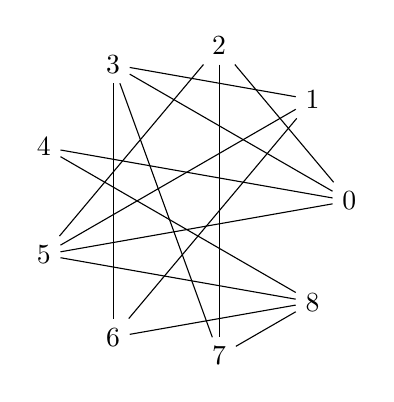
\begin{tikzpicture}
      \draw
        (0.0:2) node (0){0}
        (40.0:2) node (1){1}
        (80.0:2) node (2){2}
        (120.0:2) node (3){3}
        (160.0:2) node (4){4}
        (200.0:2) node (5){5}
        (240.0:2) node (6){6}
        (280.0:2) node (7){7}
        (320.0:2) node (8){8};
      \begin{scope}[-]
        \draw (0) to (2);
        \draw (0) to (3);
        \draw (0) to (4);
        \draw (0) to (5);
        \draw (1) to (3);
        \draw (1) to (5);
        \draw (1) to (6);
        \draw (2) to (5);
        \draw (2) to (7);
        \draw (3) to (6);
        \draw (3) to (7);
        \draw (4) to (8);
        \draw (5) to (8);
        \draw (6) to (8);
        \draw (7) to (8);
      \end{scope}
    \end{tikzpicture}
\end{figure}
\begin{itemize}
\item signature: 011110000101100001010001100001001011
\item g: Graph with 9 nodes and 15 edges
\item order: 9
\item size: 15
\item max degree: 4
\item degrees: 2,3,3,3,3,4,4,4,4
\item is tree: 0
\item is bipartite: 0
\item has bridge: 0
\item is chordal: 0
\item is complete: 0
\item min cycle basis weight: 26
\item min cycle basis size: 7
\item diameter: 3
\item radius: 2
\item is eulerian: 0
\item is planar: 0
\item number of faces: 8
\item is regular: 0
\item p3: 31
\item p4: 41
\item property hash: cad6bd599f14d9301718dfbed54ffdfd74e486cd8907d333ea55873ec30c3546
\end{itemize}
\newpage
\begin{figure}
  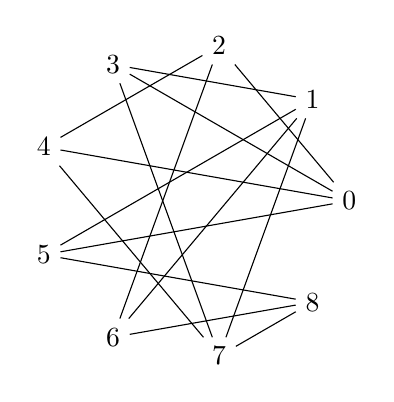
\begin{tikzpicture}
      \draw
        (0.0:2) node (0){0}
        (40.0:2) node (1){1}
        (80.0:2) node (2){2}
        (120.0:2) node (3){3}
        (160.0:2) node (4){4}
        (200.0:2) node (5){5}
        (240.0:2) node (6){6}
        (280.0:2) node (7){7}
        (320.0:2) node (8){8};
      \begin{scope}[-]
        \draw (0) to (2);
        \draw (0) to (3);
        \draw (0) to (4);
        \draw (0) to (5);
        \draw (1) to (3);
        \draw (1) to (5);
        \draw (1) to (6);
        \draw (1) to (7);
        \draw (2) to (4);
        \draw (2) to (6);
        \draw (3) to (7);
        \draw (4) to (7);
        \draw (5) to (8);
        \draw (6) to (8);
        \draw (7) to (8);
      \end{scope}
    \end{tikzpicture}
\end{figure}
\begin{itemize}
\item signature: 011110000101110010100000100010001011
\item g: Graph with 9 nodes and 15 edges
\item order: 9
\item size: 15
\item max degree: 4
\item degrees: 3,3,3,3,3,3,4,4,4
\item is tree: 0
\item is bipartite: 0
\item has bridge: 0
\item is chordal: 0
\item is complete: 0
\item min cycle basis weight: 27
\item min cycle basis size: 7
\item diameter: 2
\item radius: 2
\item is eulerian: 0
\item is planar: 0
\item number of faces: 8
\item is regular: 0
\item p3: 30
\item p4: 41
\item property hash: b6f6a327b9baa268e775c50019e551ca0e695cf2ca30abffe3490e71305c1636
\end{itemize}
\newpage
\begin{figure}
  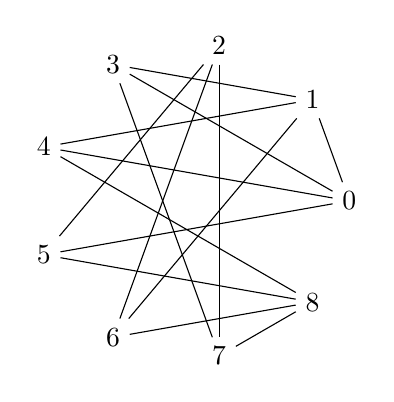
\begin{tikzpicture}
      \draw
        (0.0:2) node (0){0}
        (40.0:2) node (1){1}
        (80.0:2) node (2){2}
        (120.0:2) node (3){3}
        (160.0:2) node (4){4}
        (200.0:2) node (5){5}
        (240.0:2) node (6){6}
        (280.0:2) node (7){7}
        (320.0:2) node (8){8};
      \begin{scope}[-]
        \draw (0) to (1);
        \draw (0) to (3);
        \draw (0) to (4);
        \draw (0) to (5);
        \draw (1) to (3);
        \draw (1) to (4);
        \draw (1) to (6);
        \draw (2) to (5);
        \draw (2) to (6);
        \draw (2) to (7);
        \draw (3) to (7);
        \draw (4) to (8);
        \draw (5) to (8);
        \draw (6) to (8);
        \draw (7) to (8);
      \end{scope}
    \end{tikzpicture}
\end{figure}
\begin{itemize}
\item signature: 101110000110100001110000100001001011
\item g: Graph with 9 nodes and 15 edges
\item order: 9
\item size: 15
\item max degree: 4
\item degrees: 3,3,3,3,3,3,4,4,4
\item is tree: 0
\item is bipartite: 0
\item has bridge: 0
\item is chordal: 0
\item is complete: 0
\item min cycle basis weight: 27
\item min cycle basis size: 7
\item diameter: 3
\item radius: 2
\item is eulerian: 0
\item is planar: 0
\item number of faces: 8
\item is regular: 0
\item p3: 30
\item p4: 41
\item property hash: a6eb689b5043c32ae41fb621aaee69fd9202162a3e9dc7441c02af67b44a9fb2
\end{itemize}
\newpage
\begin{figure}
  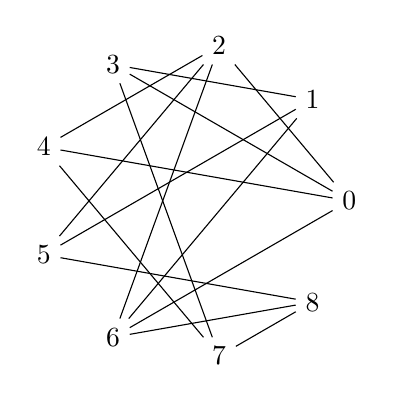
\begin{tikzpicture}
      \draw
        (0.0:2) node (0){0}
        (40.0:2) node (1){1}
        (80.0:2) node (2){2}
        (120.0:2) node (3){3}
        (160.0:2) node (4){4}
        (200.0:2) node (5){5}
        (240.0:2) node (6){6}
        (280.0:2) node (7){7}
        (320.0:2) node (8){8};
      \begin{scope}[-]
        \draw (0) to (2);
        \draw (0) to (3);
        \draw (0) to (4);
        \draw (0) to (6);
        \draw (1) to (3);
        \draw (1) to (5);
        \draw (1) to (6);
        \draw (2) to (4);
        \draw (2) to (5);
        \draw (2) to (6);
        \draw (3) to (7);
        \draw (4) to (7);
        \draw (5) to (8);
        \draw (6) to (8);
        \draw (7) to (8);
      \end{scope}
    \end{tikzpicture}
\end{figure}
\begin{itemize}
\item signature: 011101000101100011100000100010001011
\item g: Graph with 9 nodes and 15 edges
\item order: 9
\item size: 15
\item max degree: 4
\item degrees: 3,3,3,3,3,3,4,4,4
\item is tree: 0
\item is bipartite: 0
\item has bridge: 0
\item is chordal: 0
\item is complete: 0
\item min cycle basis weight: 27
\item min cycle basis size: 7
\item diameter: 3
\item radius: 2
\item is eulerian: 0
\item is planar: 0
\item number of faces: 8
\item is regular: 0
\item p3: 30
\item p4: 41
\item property hash: a6eb689b5043c32ae41fb621aaee69fd9202162a3e9dc7441c02af67b44a9fb2
\end{itemize}
\newpage
\begin{figure}
  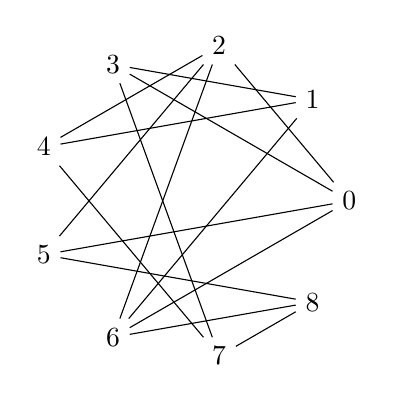
\begin{tikzpicture}
      \draw
        (0.0:2) node (0){0}
        (40.0:2) node (1){1}
        (80.0:2) node (2){2}
        (120.0:2) node (3){3}
        (160.0:2) node (4){4}
        (200.0:2) node (5){5}
        (240.0:2) node (6){6}
        (280.0:2) node (7){7}
        (320.0:2) node (8){8};
      \begin{scope}[-]
        \draw (0) to (2);
        \draw (0) to (3);
        \draw (0) to (5);
        \draw (0) to (6);
        \draw (1) to (3);
        \draw (1) to (4);
        \draw (1) to (6);
        \draw (2) to (4);
        \draw (2) to (5);
        \draw (2) to (6);
        \draw (3) to (7);
        \draw (4) to (7);
        \draw (5) to (8);
        \draw (6) to (8);
        \draw (7) to (8);
      \end{scope}
    \end{tikzpicture}
\end{figure}
\begin{itemize}
\item signature: 011011000110100011100000100010001011
\item g: Graph with 9 nodes and 15 edges
\item order: 9
\item size: 15
\item max degree: 4
\item degrees: 3,3,3,3,3,3,4,4,4
\item is tree: 0
\item is bipartite: 0
\item has bridge: 0
\item is chordal: 0
\item is complete: 0
\item min cycle basis weight: 27
\item min cycle basis size: 7
\item diameter: 3
\item radius: 2
\item is eulerian: 0
\item is planar: 0
\item number of faces: 8
\item is regular: 0
\item p3: 30
\item p4: 41
\item property hash: a6eb689b5043c32ae41fb621aaee69fd9202162a3e9dc7441c02af67b44a9fb2
\end{itemize}
\newpage
\begin{figure}
  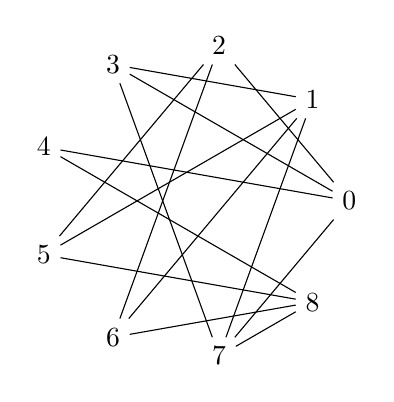
\begin{tikzpicture}
      \draw
        (0.0:2) node (0){0}
        (40.0:2) node (1){1}
        (80.0:2) node (2){2}
        (120.0:2) node (3){3}
        (160.0:2) node (4){4}
        (200.0:2) node (5){5}
        (240.0:2) node (6){6}
        (280.0:2) node (7){7}
        (320.0:2) node (8){8};
      \begin{scope}[-]
        \draw (0) to (2);
        \draw (0) to (3);
        \draw (0) to (4);
        \draw (0) to (7);
        \draw (1) to (3);
        \draw (1) to (5);
        \draw (1) to (6);
        \draw (1) to (7);
        \draw (2) to (5);
        \draw (2) to (6);
        \draw (3) to (7);
        \draw (4) to (8);
        \draw (5) to (8);
        \draw (6) to (8);
        \draw (7) to (8);
      \end{scope}
    \end{tikzpicture}
\end{figure}
\begin{itemize}
\item signature: 011100100101110001100000100001001011
\item g: Graph with 9 nodes and 15 edges
\item order: 9
\item size: 15
\item max degree: 4
\item degrees: 2,3,3,3,3,4,4,4,4
\item is tree: 0
\item is bipartite: 0
\item has bridge: 0
\item is chordal: 0
\item is complete: 0
\item min cycle basis weight: 27
\item min cycle basis size: 7
\item diameter: 3
\item radius: 2
\item is eulerian: 0
\item is planar: 0
\item number of faces: 8
\item is regular: 0
\item p3: 31
\item p4: 41
\item property hash: 604bb4afb2448bed0527b1e8fb57748dbccd0a08f573218177e50eb4d5f8e654
\end{itemize}
\newpage
\begin{figure}
  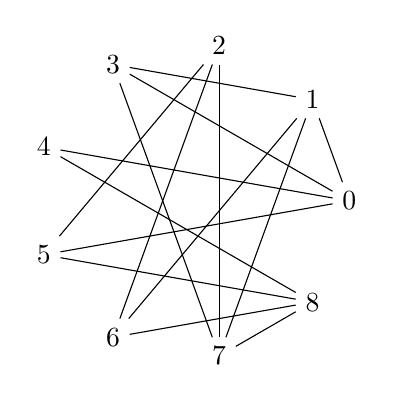
\begin{tikzpicture}
      \draw
        (0.0:2) node (0){0}
        (40.0:2) node (1){1}
        (80.0:2) node (2){2}
        (120.0:2) node (3){3}
        (160.0:2) node (4){4}
        (200.0:2) node (5){5}
        (240.0:2) node (6){6}
        (280.0:2) node (7){7}
        (320.0:2) node (8){8};
      \begin{scope}[-]
        \draw (0) to (1);
        \draw (0) to (3);
        \draw (0) to (4);
        \draw (0) to (5);
        \draw (1) to (3);
        \draw (1) to (6);
        \draw (1) to (7);
        \draw (2) to (5);
        \draw (2) to (6);
        \draw (2) to (7);
        \draw (3) to (7);
        \draw (4) to (8);
        \draw (5) to (8);
        \draw (6) to (8);
        \draw (7) to (8);
      \end{scope}
    \end{tikzpicture}
\end{figure}
\begin{itemize}
\item signature: 101110000100110001110000100001001011
\item g: Graph with 9 nodes and 15 edges
\item order: 9
\item size: 15
\item max degree: 4
\item degrees: 2,3,3,3,3,4,4,4,4
\item is tree: 0
\item is bipartite: 0
\item has bridge: 0
\item is chordal: 0
\item is complete: 0
\item min cycle basis weight: 27
\item min cycle basis size: 7
\item diameter: 3
\item radius: 2
\item is eulerian: 0
\item is planar: 0
\item number of faces: 8
\item is regular: 0
\item p3: 31
\item p4: 41
\item property hash: 604bb4afb2448bed0527b1e8fb57748dbccd0a08f573218177e50eb4d5f8e654
\end{itemize}
\newpage
\begin{figure}
  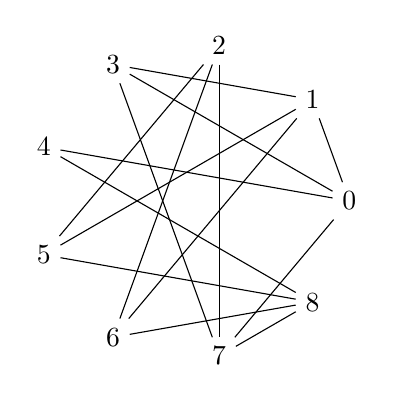
\begin{tikzpicture}
      \draw
        (0.0:2) node (0){0}
        (40.0:2) node (1){1}
        (80.0:2) node (2){2}
        (120.0:2) node (3){3}
        (160.0:2) node (4){4}
        (200.0:2) node (5){5}
        (240.0:2) node (6){6}
        (280.0:2) node (7){7}
        (320.0:2) node (8){8};
      \begin{scope}[-]
        \draw (0) to (1);
        \draw (0) to (3);
        \draw (0) to (4);
        \draw (0) to (7);
        \draw (1) to (3);
        \draw (1) to (5);
        \draw (1) to (6);
        \draw (2) to (5);
        \draw (2) to (6);
        \draw (2) to (7);
        \draw (3) to (7);
        \draw (4) to (8);
        \draw (5) to (8);
        \draw (6) to (8);
        \draw (7) to (8);
      \end{scope}
    \end{tikzpicture}
\end{figure}
\begin{itemize}
\item signature: 101100100101100001110000100001001011
\item g: Graph with 9 nodes and 15 edges
\item order: 9
\item size: 15
\item max degree: 4
\item degrees: 2,3,3,3,3,4,4,4,4
\item is tree: 0
\item is bipartite: 0
\item has bridge: 0
\item is chordal: 0
\item is complete: 0
\item min cycle basis weight: 27
\item min cycle basis size: 7
\item diameter: 3
\item radius: 2
\item is eulerian: 0
\item is planar: 0
\item number of faces: 8
\item is regular: 0
\item p3: 31
\item p4: 41
\item property hash: 604bb4afb2448bed0527b1e8fb57748dbccd0a08f573218177e50eb4d5f8e654
\end{itemize}
\newpage
\begin{figure}
  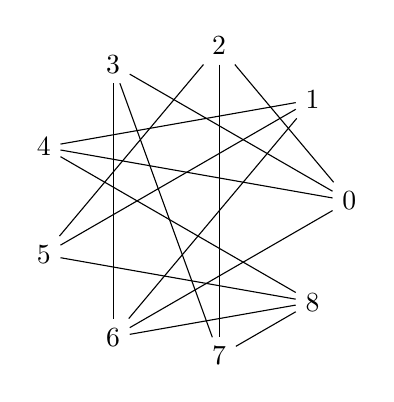
\begin{tikzpicture}
      \draw
        (0.0:2) node (0){0}
        (40.0:2) node (1){1}
        (80.0:2) node (2){2}
        (120.0:2) node (3){3}
        (160.0:2) node (4){4}
        (200.0:2) node (5){5}
        (240.0:2) node (6){6}
        (280.0:2) node (7){7}
        (320.0:2) node (8){8};
      \begin{scope}[-]
        \draw (0) to (2);
        \draw (0) to (3);
        \draw (0) to (4);
        \draw (0) to (6);
        \draw (1) to (4);
        \draw (1) to (5);
        \draw (1) to (6);
        \draw (2) to (5);
        \draw (2) to (7);
        \draw (3) to (6);
        \draw (3) to (7);
        \draw (4) to (8);
        \draw (5) to (8);
        \draw (6) to (8);
        \draw (7) to (8);
      \end{scope}
    \end{tikzpicture}
\end{figure}
\begin{itemize}
\item signature: 011101000011100001010001100001001011
\item g: Graph with 9 nodes and 15 edges
\item order: 9
\item size: 15
\item max degree: 4
\item degrees: 3,3,3,3,3,3,4,4,4
\item is tree: 0
\item is bipartite: 0
\item has bridge: 0
\item is chordal: 0
\item is complete: 0
\item min cycle basis weight: 27
\item min cycle basis size: 7
\item diameter: 3
\item radius: 2
\item is eulerian: 0
\item is planar: 0
\item number of faces: 8
\item is regular: 0
\item p3: 33
\item p4: 41
\item property hash: 9944ca3cadb2a758b71f4c48c393410fd2e9898daaa72eedc2bc833557f58314
\end{itemize}
\newpage
\begin{figure}
  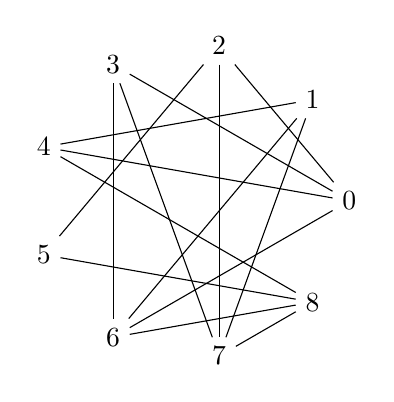
\begin{tikzpicture}
      \draw
        (0.0:2) node (0){0}
        (40.0:2) node (1){1}
        (80.0:2) node (2){2}
        (120.0:2) node (3){3}
        (160.0:2) node (4){4}
        (200.0:2) node (5){5}
        (240.0:2) node (6){6}
        (280.0:2) node (7){7}
        (320.0:2) node (8){8};
      \begin{scope}[-]
        \draw (0) to (2);
        \draw (0) to (3);
        \draw (0) to (4);
        \draw (0) to (6);
        \draw (1) to (4);
        \draw (1) to (6);
        \draw (1) to (7);
        \draw (2) to (5);
        \draw (2) to (7);
        \draw (3) to (6);
        \draw (3) to (7);
        \draw (4) to (8);
        \draw (5) to (8);
        \draw (6) to (8);
        \draw (7) to (8);
      \end{scope}
    \end{tikzpicture}
\end{figure}
\begin{itemize}
\item signature: 011101000010110001010001100001001011
\item g: Graph with 9 nodes and 15 edges
\item order: 9
\item size: 15
\item max degree: 4
\item degrees: 2,3,3,3,3,4,4,4,4
\item is tree: 0
\item is bipartite: 0
\item has bridge: 0
\item is chordal: 0
\item is complete: 0
\item min cycle basis weight: 27
\item min cycle basis size: 7
\item diameter: 3
\item radius: 2
\item is eulerian: 0
\item is planar: 0
\item number of faces: 8
\item is regular: 0
\item p3: 34
\item p4: 41
\item property hash: d1b6235d989b534b202e2977d8b6439dc9a78fcbcd891c5884ca69da1582af18
\end{itemize}
\newpage
\begin{figure}
  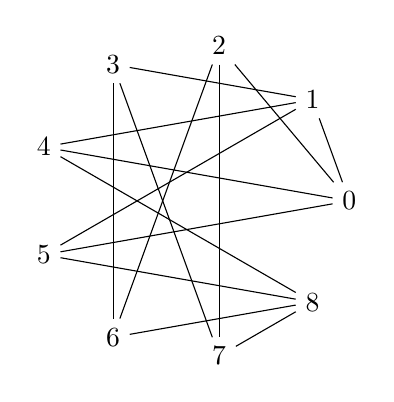
\begin{tikzpicture}
      \draw
        (0.0:2) node (0){0}
        (40.0:2) node (1){1}
        (80.0:2) node (2){2}
        (120.0:2) node (3){3}
        (160.0:2) node (4){4}
        (200.0:2) node (5){5}
        (240.0:2) node (6){6}
        (280.0:2) node (7){7}
        (320.0:2) node (8){8};
      \begin{scope}[-]
        \draw (0) to (1);
        \draw (0) to (2);
        \draw (0) to (4);
        \draw (0) to (5);
        \draw (1) to (3);
        \draw (1) to (4);
        \draw (1) to (5);
        \draw (2) to (6);
        \draw (2) to (7);
        \draw (3) to (6);
        \draw (3) to (7);
        \draw (4) to (8);
        \draw (5) to (8);
        \draw (6) to (8);
        \draw (7) to (8);
      \end{scope}
    \end{tikzpicture}
\end{figure}
\begin{itemize}
\item signature: 110110000111000000110001100001001011
\item g: Graph with 9 nodes and 15 edges
\item order: 9
\item size: 15
\item max degree: 4
\item degrees: 3,3,3,3,3,3,4,4,4
\item is tree: 0
\item is bipartite: 0
\item has bridge: 0
\item is chordal: 0
\item is complete: 0
\item min cycle basis weight: 28
\item min cycle basis size: 7
\item diameter: 2
\item radius: 2
\item is eulerian: 0
\item is planar: 0
\item number of faces: 8
\item is regular: 0
\item p3: 30
\item p4: 41
\item property hash: 4d3d569f86d36b353a0f8d9e4eea9a612b5ed1eeb8ad86ed7d985b3a56f07acc
\end{itemize}
\newpage
\begin{figure}
  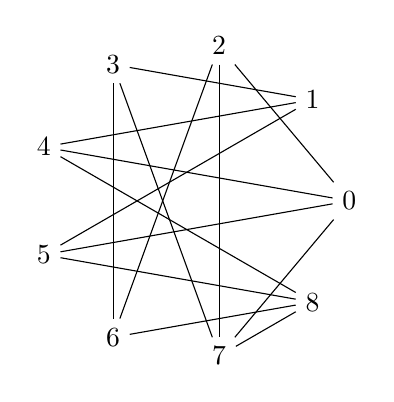
\begin{tikzpicture}
      \draw
        (0.0:2) node (0){0}
        (40.0:2) node (1){1}
        (80.0:2) node (2){2}
        (120.0:2) node (3){3}
        (160.0:2) node (4){4}
        (200.0:2) node (5){5}
        (240.0:2) node (6){6}
        (280.0:2) node (7){7}
        (320.0:2) node (8){8};
      \begin{scope}[-]
        \draw (0) to (2);
        \draw (0) to (4);
        \draw (0) to (5);
        \draw (0) to (7);
        \draw (1) to (3);
        \draw (1) to (4);
        \draw (1) to (5);
        \draw (2) to (6);
        \draw (2) to (7);
        \draw (3) to (6);
        \draw (3) to (7);
        \draw (4) to (8);
        \draw (5) to (8);
        \draw (6) to (8);
        \draw (7) to (8);
      \end{scope}
    \end{tikzpicture}
\end{figure}
\begin{itemize}
\item signature: 010110100111000000110001100001001011
\item g: Graph with 9 nodes and 15 edges
\item order: 9
\item size: 15
\item max degree: 4
\item degrees: 3,3,3,3,3,3,4,4,4
\item is tree: 0
\item is bipartite: 0
\item has bridge: 0
\item is chordal: 0
\item is complete: 0
\item min cycle basis weight: 28
\item min cycle basis size: 7
\item diameter: 3
\item radius: 2
\item is eulerian: 0
\item is planar: 0
\item number of faces: 8
\item is regular: 0
\item p3: 33
\item p4: 41
\item property hash: b0ac8b9f8fdd3b687da15a0894bae81cc7dc75030b731c8a826b1516a8cf5c5e
\end{itemize}
\newpage
\begin{figure}
  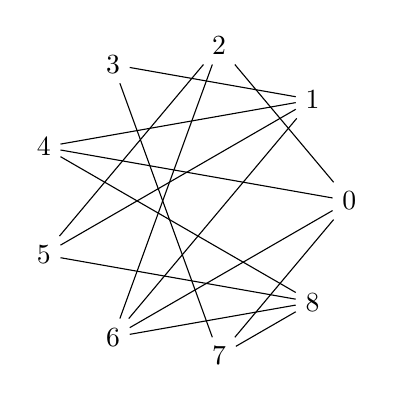
\begin{tikzpicture}
      \draw
        (0.0:2) node (0){0}
        (40.0:2) node (1){1}
        (80.0:2) node (2){2}
        (120.0:2) node (3){3}
        (160.0:2) node (4){4}
        (200.0:2) node (5){5}
        (240.0:2) node (6){6}
        (280.0:2) node (7){7}
        (320.0:2) node (8){8};
      \begin{scope}[-]
        \draw (0) to (2);
        \draw (0) to (4);
        \draw (0) to (6);
        \draw (0) to (7);
        \draw (1) to (3);
        \draw (1) to (4);
        \draw (1) to (5);
        \draw (1) to (6);
        \draw (2) to (5);
        \draw (2) to (6);
        \draw (3) to (7);
        \draw (4) to (8);
        \draw (5) to (8);
        \draw (6) to (8);
        \draw (7) to (8);
      \end{scope}
    \end{tikzpicture}
\end{figure}
\begin{itemize}
\item signature: 010101100111100001100000100001001011
\item g: Graph with 9 nodes and 15 edges
\item order: 9
\item size: 15
\item max degree: 4
\item degrees: 2,3,3,3,3,4,4,4,4
\item is tree: 0
\item is bipartite: 0
\item has bridge: 0
\item is chordal: 0
\item is complete: 0
\item min cycle basis weight: 28
\item min cycle basis size: 7
\item diameter: 3
\item radius: 2
\item is eulerian: 0
\item is planar: 0
\item number of faces: 8
\item is regular: 0
\item p3: 34
\item p4: 41
\item property hash: c7d34b19f745f6105906834ebb4cd2161b2fa39edd67e234aa0e24507c5972c5
\end{itemize}
\newpage
\begin{figure}
  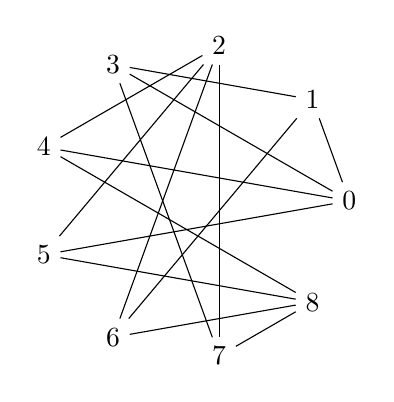
\begin{tikzpicture}
      \draw
        (0.0:2) node (0){0}
        (40.0:2) node (1){1}
        (80.0:2) node (2){2}
        (120.0:2) node (3){3}
        (160.0:2) node (4){4}
        (200.0:2) node (5){5}
        (240.0:2) node (6){6}
        (280.0:2) node (7){7}
        (320.0:2) node (8){8};
      \begin{scope}[-]
        \draw (0) to (1);
        \draw (0) to (3);
        \draw (0) to (4);
        \draw (0) to (5);
        \draw (1) to (3);
        \draw (1) to (6);
        \draw (2) to (4);
        \draw (2) to (5);
        \draw (2) to (6);
        \draw (2) to (7);
        \draw (3) to (7);
        \draw (4) to (8);
        \draw (5) to (8);
        \draw (6) to (8);
        \draw (7) to (8);
      \end{scope}
    \end{tikzpicture}
\end{figure}
\begin{itemize}
\item signature: 101110000100100011110000100001001011
\item g: Graph with 9 nodes and 15 edges
\item order: 9
\item size: 15
\item max degree: 4
\item degrees: 3,3,3,3,3,3,4,4,4
\item is tree: 0
\item is bipartite: 0
\item has bridge: 0
\item is chordal: 0
\item is complete: 0
\item min cycle basis weight: 29
\item min cycle basis size: 7
\item diameter: 2
\item radius: 2
\item is eulerian: 0
\item is planar: 0
\item number of faces: 8
\item is regular: 0
\item p3: 33
\item p4: 41
\item property hash: de1f859b9a80f9d01560615b39d7e3d79c709a1e22530347bb070e4d6c1b7c4b
\end{itemize}
\newpage
\begin{figure}
  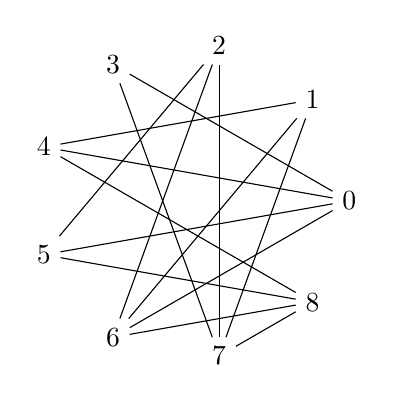
\begin{tikzpicture}
      \draw
        (0.0:2) node (0){0}
        (40.0:2) node (1){1}
        (80.0:2) node (2){2}
        (120.0:2) node (3){3}
        (160.0:2) node (4){4}
        (200.0:2) node (5){5}
        (240.0:2) node (6){6}
        (280.0:2) node (7){7}
        (320.0:2) node (8){8};
      \begin{scope}[-]
        \draw (0) to (3);
        \draw (0) to (4);
        \draw (0) to (5);
        \draw (0) to (6);
        \draw (1) to (4);
        \draw (1) to (6);
        \draw (1) to (7);
        \draw (2) to (5);
        \draw (2) to (6);
        \draw (2) to (7);
        \draw (3) to (7);
        \draw (4) to (8);
        \draw (5) to (8);
        \draw (6) to (8);
        \draw (7) to (8);
      \end{scope}
    \end{tikzpicture}
\end{figure}
\begin{itemize}
\item signature: 001111000010110001110000100001001011
\item g: Graph with 9 nodes and 15 edges
\item order: 9
\item size: 15
\item max degree: 4
\item degrees: 2,3,3,3,3,4,4,4,4
\item is tree: 0
\item is bipartite: 0
\item has bridge: 0
\item is chordal: 0
\item is complete: 0
\item min cycle basis weight: 29
\item min cycle basis size: 7
\item diameter: 3
\item radius: 2
\item is eulerian: 0
\item is planar: 0
\item number of faces: 8
\item is regular: 0
\item p3: 37
\item p4: 41
\item property hash: d67fa328f5a67a591aaed78a5b635b4318d2734a6b6eaeb988b9a1e30f1236d6
\end{itemize}
\newpage
\begin{figure}
  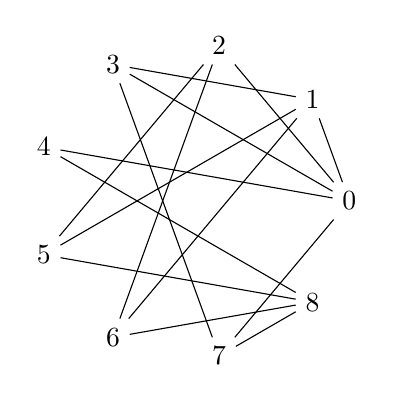
\begin{tikzpicture}
      \draw
        (0.0:2) node (0){0}
        (40.0:2) node (1){1}
        (80.0:2) node (2){2}
        (120.0:2) node (3){3}
        (160.0:2) node (4){4}
        (200.0:2) node (5){5}
        (240.0:2) node (6){6}
        (280.0:2) node (7){7}
        (320.0:2) node (8){8};
      \begin{scope}[-]
        \draw (0) to (1);
        \draw (0) to (2);
        \draw (0) to (3);
        \draw (0) to (4);
        \draw (0) to (7);
        \draw (1) to (3);
        \draw (1) to (5);
        \draw (1) to (6);
        \draw (2) to (5);
        \draw (2) to (6);
        \draw (3) to (7);
        \draw (4) to (8);
        \draw (5) to (8);
        \draw (6) to (8);
        \draw (7) to (8);
      \end{scope}
    \end{tikzpicture}
\end{figure}
\begin{itemize}
\item signature: 111100100101100001100000100001001011
\item g: Graph with 9 nodes and 15 edges
\item order: 9
\item size: 15
\item max degree: 5
\item degrees: 2,3,3,3,3,3,4,4,5
\item is tree: 0
\item is bipartite: 0
\item has bridge: 0
\item is chordal: 0
\item is complete: 0
\item min cycle basis weight: 27
\item min cycle basis size: 7
\item diameter: 2
\item radius: 2
\item is eulerian: 0
\item is planar: 0
\item number of faces: 8
\item is regular: 0
\item p3: 32
\item p4: 41
\item property hash: b2ae01f501c3699e4f5b4f7b994d7f4e8bddd90ff265ab6f01fa46c9db365933
\end{itemize}
\newpage
\begin{figure}
  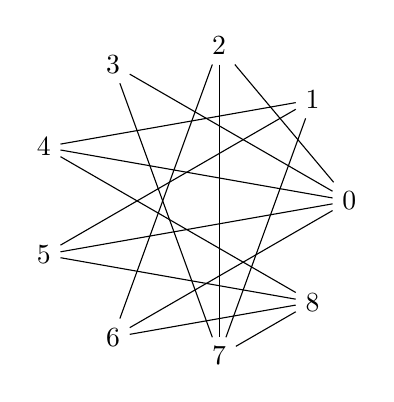
\begin{tikzpicture}
      \draw
        (0.0:2) node (0){0}
        (40.0:2) node (1){1}
        (80.0:2) node (2){2}
        (120.0:2) node (3){3}
        (160.0:2) node (4){4}
        (200.0:2) node (5){5}
        (240.0:2) node (6){6}
        (280.0:2) node (7){7}
        (320.0:2) node (8){8};
      \begin{scope}[-]
        \draw (0) to (2);
        \draw (0) to (3);
        \draw (0) to (4);
        \draw (0) to (5);
        \draw (0) to (6);
        \draw (1) to (4);
        \draw (1) to (5);
        \draw (1) to (7);
        \draw (2) to (6);
        \draw (2) to (7);
        \draw (3) to (7);
        \draw (4) to (8);
        \draw (5) to (8);
        \draw (6) to (8);
        \draw (7) to (8);
      \end{scope}
    \end{tikzpicture}
\end{figure}
\begin{itemize}
\item signature: 011111000011010000110000100001001011
\item g: Graph with 9 nodes and 15 edges
\item order: 9
\item size: 15
\item max degree: 5
\item degrees: 2,3,3,3,3,3,4,4,5
\item is tree: 0
\item is bipartite: 0
\item has bridge: 0
\item is chordal: 0
\item is complete: 0
\item min cycle basis weight: 27
\item min cycle basis size: 7
\item diameter: 3
\item radius: 2
\item is eulerian: 0
\item is planar: 0
\item number of faces: 8
\item is regular: 0
\item p3: 35
\item p4: 41
\item property hash: 7c0164ce8e86ce25c4408247160fa5f96b725e1d2fe4bd57d7bde38adfe860c8
\end{itemize}
\newpage
\begin{figure}
  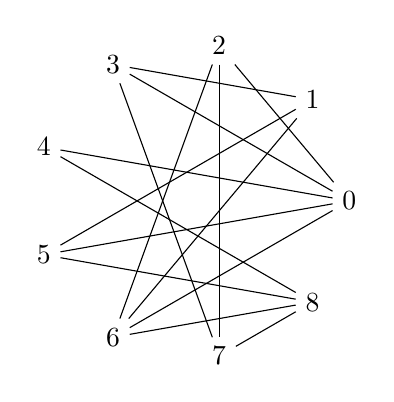
\begin{tikzpicture}
      \draw
        (0.0:2) node (0){0}
        (40.0:2) node (1){1}
        (80.0:2) node (2){2}
        (120.0:2) node (3){3}
        (160.0:2) node (4){4}
        (200.0:2) node (5){5}
        (240.0:2) node (6){6}
        (280.0:2) node (7){7}
        (320.0:2) node (8){8};
      \begin{scope}[-]
        \draw (0) to (2);
        \draw (0) to (3);
        \draw (0) to (4);
        \draw (0) to (5);
        \draw (0) to (6);
        \draw (1) to (3);
        \draw (1) to (5);
        \draw (1) to (6);
        \draw (2) to (6);
        \draw (2) to (7);
        \draw (3) to (7);
        \draw (4) to (8);
        \draw (5) to (8);
        \draw (6) to (8);
        \draw (7) to (8);
      \end{scope}
    \end{tikzpicture}
\end{figure}
\begin{itemize}
\item signature: 011111000101100000110000100001001011
\item g: Graph with 9 nodes and 15 edges
\item order: 9
\item size: 15
\item max degree: 5
\item degrees: 2,3,3,3,3,3,4,4,5
\item is tree: 0
\item is bipartite: 0
\item has bridge: 0
\item is chordal: 0
\item is complete: 0
\item min cycle basis weight: 27
\item min cycle basis size: 7
\item diameter: 3
\item radius: 2
\item is eulerian: 0
\item is planar: 0
\item number of faces: 8
\item is regular: 0
\item p3: 35
\item p4: 41
\item property hash: 7c0164ce8e86ce25c4408247160fa5f96b725e1d2fe4bd57d7bde38adfe860c8
\end{itemize}
\newpage
\begin{figure}
  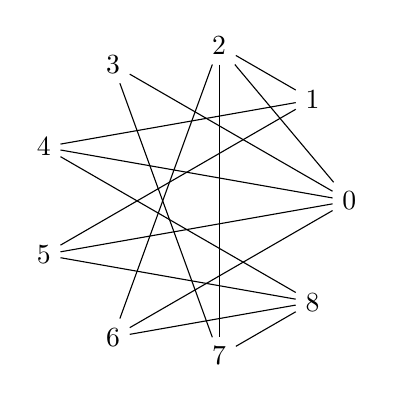
\begin{tikzpicture}
      \draw
        (0.0:2) node (0){0}
        (40.0:2) node (1){1}
        (80.0:2) node (2){2}
        (120.0:2) node (3){3}
        (160.0:2) node (4){4}
        (200.0:2) node (5){5}
        (240.0:2) node (6){6}
        (280.0:2) node (7){7}
        (320.0:2) node (8){8};
      \begin{scope}[-]
        \draw (0) to (2);
        \draw (0) to (3);
        \draw (0) to (4);
        \draw (0) to (5);
        \draw (0) to (6);
        \draw (1) to (2);
        \draw (1) to (4);
        \draw (1) to (5);
        \draw (2) to (6);
        \draw (2) to (7);
        \draw (3) to (7);
        \draw (4) to (8);
        \draw (5) to (8);
        \draw (6) to (8);
        \draw (7) to (8);
      \end{scope}
    \end{tikzpicture}
\end{figure}
\begin{itemize}
\item signature: 011111001011000000110000100001001011
\item g: Graph with 9 nodes and 15 edges
\item order: 9
\item size: 15
\item max degree: 5
\item degrees: 2,3,3,3,3,3,4,4,5
\item is tree: 0
\item is bipartite: 0
\item has bridge: 0
\item is chordal: 0
\item is complete: 0
\item min cycle basis weight: 27
\item min cycle basis size: 7
\item diameter: 3
\item radius: 2
\item is eulerian: 0
\item is planar: 0
\item number of faces: 8
\item is regular: 0
\item p3: 35
\item p4: 41
\item property hash: 7c0164ce8e86ce25c4408247160fa5f96b725e1d2fe4bd57d7bde38adfe860c8
\end{itemize}
\newpage
\begin{figure}
  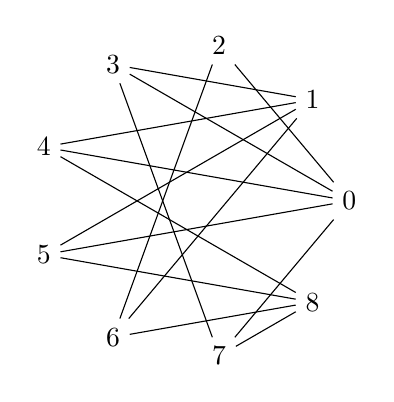
\begin{tikzpicture}
      \draw
        (0.0:2) node (0){0}
        (40.0:2) node (1){1}
        (80.0:2) node (2){2}
        (120.0:2) node (3){3}
        (160.0:2) node (4){4}
        (200.0:2) node (5){5}
        (240.0:2) node (6){6}
        (280.0:2) node (7){7}
        (320.0:2) node (8){8};
      \begin{scope}[-]
        \draw (0) to (2);
        \draw (0) to (3);
        \draw (0) to (4);
        \draw (0) to (5);
        \draw (0) to (7);
        \draw (1) to (3);
        \draw (1) to (4);
        \draw (1) to (5);
        \draw (1) to (6);
        \draw (2) to (6);
        \draw (3) to (7);
        \draw (4) to (8);
        \draw (5) to (8);
        \draw (6) to (8);
        \draw (7) to (8);
      \end{scope}
    \end{tikzpicture}
\end{figure}
\begin{itemize}
\item signature: 011110100111100000100000100001001011
\item g: Graph with 9 nodes and 15 edges
\item order: 9
\item size: 15
\item max degree: 5
\item degrees: 2,3,3,3,3,3,4,4,5
\item is tree: 0
\item is bipartite: 0
\item has bridge: 0
\item is chordal: 0
\item is complete: 0
\item min cycle basis weight: 28
\item min cycle basis size: 7
\item diameter: 2
\item radius: 2
\item is eulerian: 0
\item is planar: 0
\item number of faces: 8
\item is regular: 0
\item p3: 35
\item p4: 41
\item property hash: 37f8bce98d8be4e236ab6d233a58e782956ac747157c095e22198fa9f9715e39
\end{itemize}
\newpage
\begin{figure}
  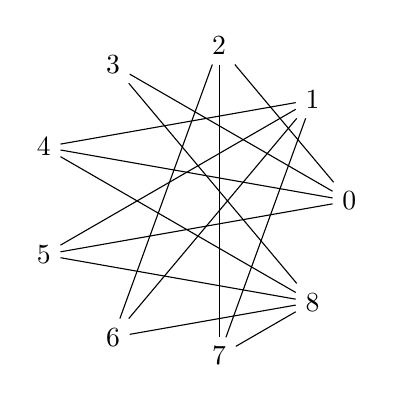
\begin{tikzpicture}
      \draw
        (0.0:2) node (0){0}
        (40.0:2) node (1){1}
        (80.0:2) node (2){2}
        (120.0:2) node (3){3}
        (160.0:2) node (4){4}
        (200.0:2) node (5){5}
        (240.0:2) node (6){6}
        (280.0:2) node (7){7}
        (320.0:2) node (8){8};
      \begin{scope}[-]
        \draw (0) to (2);
        \draw (0) to (3);
        \draw (0) to (4);
        \draw (0) to (5);
        \draw (1) to (4);
        \draw (1) to (5);
        \draw (1) to (6);
        \draw (1) to (7);
        \draw (2) to (6);
        \draw (2) to (7);
        \draw (3) to (8);
        \draw (4) to (8);
        \draw (5) to (8);
        \draw (6) to (8);
        \draw (7) to (8);
      \end{scope}
    \end{tikzpicture}
\end{figure}
\begin{itemize}
\item signature: 011110000011110000110000010001001011
\item g: Graph with 9 nodes and 15 edges
\item order: 9
\item size: 15
\item max degree: 5
\item degrees: 2,3,3,3,3,3,4,4,5
\item is tree: 0
\item is bipartite: 0
\item has bridge: 0
\item is chordal: 0
\item is complete: 0
\item min cycle basis weight: 29
\item min cycle basis size: 7
\item diameter: 3
\item radius: 2
\item is eulerian: 0
\item is planar: 0
\item number of faces: 8
\item is regular: 0
\item p3: 38
\item p4: 41
\item property hash: 50009b2e632be52dc0d2b325b72bdaa535b85638ceb05b026b144286c3f7edd7
\end{itemize}
\newpage
\begin{figure}
  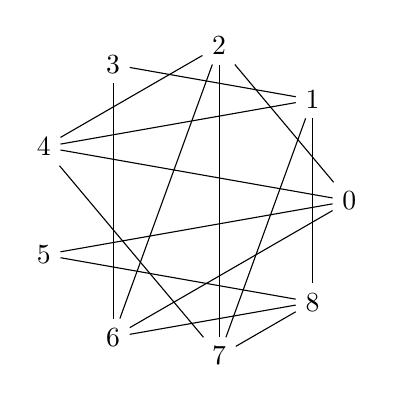
\begin{tikzpicture}
      \draw
        (0.0:2) node (0){0}
        (40.0:2) node (1){1}
        (80.0:2) node (2){2}
        (120.0:2) node (3){3}
        (160.0:2) node (4){4}
        (200.0:2) node (5){5}
        (240.0:2) node (6){6}
        (280.0:2) node (7){7}
        (320.0:2) node (8){8};
      \begin{scope}[-]
        \draw (0) to (2);
        \draw (0) to (4);
        \draw (0) to (5);
        \draw (0) to (6);
        \draw (1) to (3);
        \draw (1) to (4);
        \draw (1) to (7);
        \draw (1) to (8);
        \draw (2) to (4);
        \draw (2) to (6);
        \draw (2) to (7);
        \draw (3) to (6);
        \draw (4) to (7);
        \draw (5) to (8);
        \draw (6) to (8);
        \draw (7) to (8);
      \end{scope}
    \end{tikzpicture}
\end{figure}
\begin{itemize}
\item signature: 010111000110011010110001000010001011
\item g: Graph with 9 nodes and 16 edges
\item order: 9
\item size: 16
\item max degree: 4
\item degrees: 2,2,4,4,4,4,4,4,4
\item is tree: 0
\item is bipartite: 0
\item has bridge: 0
\item is chordal: 0
\item is complete: 0
\item min cycle basis weight: 27
\item min cycle basis size: 8
\item diameter: 3
\item radius: 2
\item is eulerian: 1
\item is planar: 0
\item number of faces: 9
\item is regular: 0
\item p3: 29
\item p4: 41
\item property hash: 952cf8995b9764c7774f7aba6b68d0d328f497bb717f80bbf2fa63c3744822c6
\end{itemize}
\newpage
\begin{figure}
  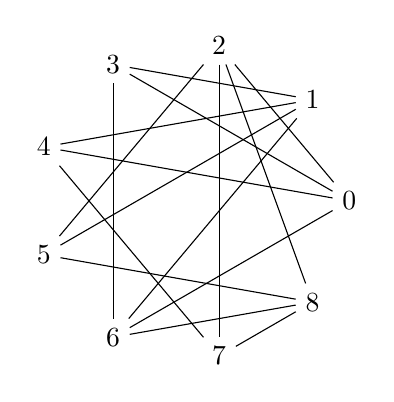
\begin{tikzpicture}
      \draw
        (0.0:2) node (0){0}
        (40.0:2) node (1){1}
        (80.0:2) node (2){2}
        (120.0:2) node (3){3}
        (160.0:2) node (4){4}
        (200.0:2) node (5){5}
        (240.0:2) node (6){6}
        (280.0:2) node (7){7}
        (320.0:2) node (8){8};
      \begin{scope}[-]
        \draw (0) to (2);
        \draw (0) to (3);
        \draw (0) to (4);
        \draw (0) to (6);
        \draw (1) to (3);
        \draw (1) to (4);
        \draw (1) to (5);
        \draw (1) to (6);
        \draw (2) to (5);
        \draw (2) to (7);
        \draw (2) to (8);
        \draw (3) to (6);
        \draw (4) to (7);
        \draw (5) to (8);
        \draw (6) to (8);
        \draw (7) to (8);
      \end{scope}
    \end{tikzpicture}
\end{figure}
\begin{itemize}
\item signature: 011101000111100001011001000010001011
\item g: Graph with 9 nodes and 16 edges
\item order: 9
\item size: 16
\item max degree: 4
\item degrees: 3,3,3,3,4,4,4,4,4
\item is tree: 0
\item is bipartite: 0
\item has bridge: 0
\item is chordal: 0
\item is complete: 0
\item min cycle basis weight: 28
\item min cycle basis size: 8
\item diameter: 3
\item radius: 2
\item is eulerian: 0
\item is planar: 0
\item number of faces: 9
\item is regular: 0
\item p3: 30
\item p4: 41
\item property hash: d2f0cef6592de3143b4622c0d30c78c8bbc2bee702d84518bdbf1ac3a9d334db
\end{itemize}
\newpage
\begin{figure}
  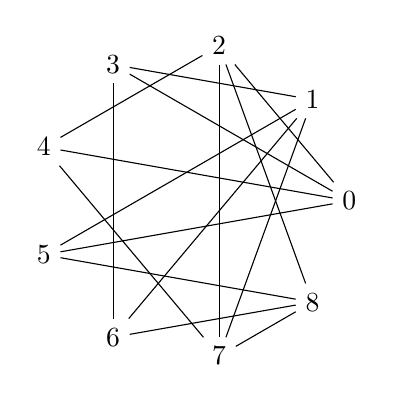
\begin{tikzpicture}
      \draw
        (0.0:2) node (0){0}
        (40.0:2) node (1){1}
        (80.0:2) node (2){2}
        (120.0:2) node (3){3}
        (160.0:2) node (4){4}
        (200.0:2) node (5){5}
        (240.0:2) node (6){6}
        (280.0:2) node (7){7}
        (320.0:2) node (8){8};
      \begin{scope}[-]
        \draw (0) to (2);
        \draw (0) to (3);
        \draw (0) to (4);
        \draw (0) to (5);
        \draw (1) to (3);
        \draw (1) to (5);
        \draw (1) to (6);
        \draw (1) to (7);
        \draw (2) to (4);
        \draw (2) to (7);
        \draw (2) to (8);
        \draw (3) to (6);
        \draw (4) to (7);
        \draw (5) to (8);
        \draw (6) to (8);
        \draw (7) to (8);
      \end{scope}
    \end{tikzpicture}
\end{figure}
\begin{itemize}
\item signature: 011110000101110010011001000010001011
\item g: Graph with 9 nodes and 16 edges
\item order: 9
\item size: 16
\item max degree: 4
\item degrees: 3,3,3,3,4,4,4,4,4
\item is tree: 0
\item is bipartite: 0
\item has bridge: 0
\item is chordal: 0
\item is complete: 0
\item min cycle basis weight: 28
\item min cycle basis size: 8
\item diameter: 3
\item radius: 2
\item is eulerian: 0
\item is planar: 0
\item number of faces: 9
\item is regular: 0
\item p3: 30
\item p4: 41
\item property hash: d2f0cef6592de3143b4622c0d30c78c8bbc2bee702d84518bdbf1ac3a9d334db
\end{itemize}
\newpage
\begin{figure}
  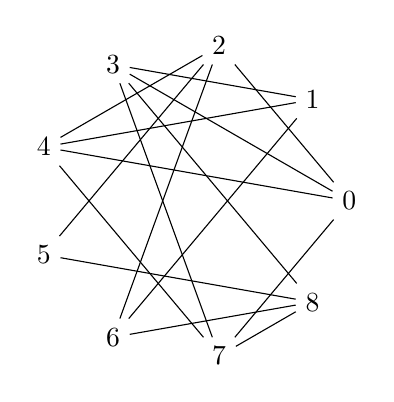
\begin{tikzpicture}
      \draw
        (0.0:2) node (0){0}
        (40.0:2) node (1){1}
        (80.0:2) node (2){2}
        (120.0:2) node (3){3}
        (160.0:2) node (4){4}
        (200.0:2) node (5){5}
        (240.0:2) node (6){6}
        (280.0:2) node (7){7}
        (320.0:2) node (8){8};
      \begin{scope}[-]
        \draw (0) to (2);
        \draw (0) to (3);
        \draw (0) to (4);
        \draw (0) to (7);
        \draw (1) to (3);
        \draw (1) to (4);
        \draw (1) to (6);
        \draw (2) to (4);
        \draw (2) to (5);
        \draw (2) to (6);
        \draw (3) to (7);
        \draw (3) to (8);
        \draw (4) to (7);
        \draw (5) to (8);
        \draw (6) to (8);
        \draw (7) to (8);
      \end{scope}
    \end{tikzpicture}
\end{figure}
\begin{itemize}
\item signature: 011100100110100011100000110010001011
\item g: Graph with 9 nodes and 16 edges
\item order: 9
\item size: 16
\item max degree: 4
\item degrees: 2,3,3,4,4,4,4,4,4
\item is tree: 0
\item is bipartite: 0
\item has bridge: 0
\item is chordal: 0
\item is complete: 0
\item min cycle basis weight: 28
\item min cycle basis size: 8
\item diameter: 3
\item radius: 2
\item is eulerian: 0
\item is planar: 0
\item number of faces: 9
\item is regular: 0
\item p3: 31
\item p4: 41
\item property hash: 4d84469c696e06bf13d189d44d9ffbdeabecfb096a0fe4add8c9ce8ba9222ada
\end{itemize}
\newpage
\begin{figure}
  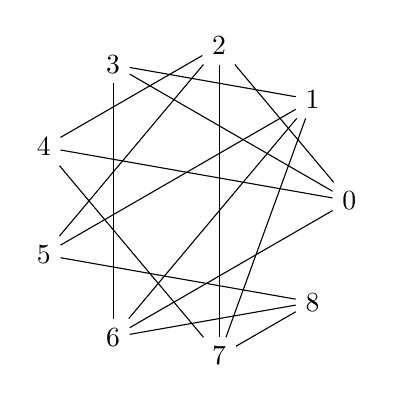
\begin{tikzpicture}
      \draw
        (0.0:2) node (0){0}
        (40.0:2) node (1){1}
        (80.0:2) node (2){2}
        (120.0:2) node (3){3}
        (160.0:2) node (4){4}
        (200.0:2) node (5){5}
        (240.0:2) node (6){6}
        (280.0:2) node (7){7}
        (320.0:2) node (8){8};
      \begin{scope}[-]
        \draw (0) to (2);
        \draw (0) to (3);
        \draw (0) to (4);
        \draw (0) to (6);
        \draw (1) to (3);
        \draw (1) to (5);
        \draw (1) to (6);
        \draw (1) to (7);
        \draw (2) to (4);
        \draw (2) to (5);
        \draw (2) to (7);
        \draw (3) to (6);
        \draw (4) to (7);
        \draw (5) to (8);
        \draw (6) to (8);
        \draw (7) to (8);
      \end{scope}
    \end{tikzpicture}
\end{figure}
\begin{itemize}
\item signature: 011101000101110011010001000010001011
\item g: Graph with 9 nodes and 16 edges
\item order: 9
\item size: 16
\item max degree: 4
\item degrees: 3,3,3,3,4,4,4,4,4
\item is tree: 0
\item is bipartite: 0
\item has bridge: 0
\item is chordal: 0
\item is complete: 0
\item min cycle basis weight: 29
\item min cycle basis size: 8
\item diameter: 2
\item radius: 2
\item is eulerian: 0
\item is planar: 0
\item number of faces: 9
\item is regular: 0
\item p3: 30
\item p4: 41
\item property hash: a99a06ab6260bfd9cc743969366a65f35a149155373f15e720d17f7c157c54ac
\end{itemize}
\newpage
\begin{figure}
  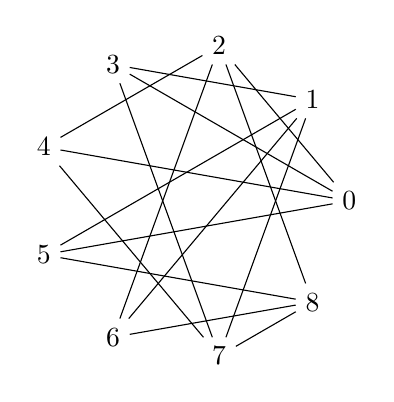
\begin{tikzpicture}
      \draw
        (0.0:2) node (0){0}
        (40.0:2) node (1){1}
        (80.0:2) node (2){2}
        (120.0:2) node (3){3}
        (160.0:2) node (4){4}
        (200.0:2) node (5){5}
        (240.0:2) node (6){6}
        (280.0:2) node (7){7}
        (320.0:2) node (8){8};
      \begin{scope}[-]
        \draw (0) to (2);
        \draw (0) to (3);
        \draw (0) to (4);
        \draw (0) to (5);
        \draw (1) to (3);
        \draw (1) to (5);
        \draw (1) to (6);
        \draw (1) to (7);
        \draw (2) to (4);
        \draw (2) to (6);
        \draw (2) to (8);
        \draw (3) to (7);
        \draw (4) to (7);
        \draw (5) to (8);
        \draw (6) to (8);
        \draw (7) to (8);
      \end{scope}
    \end{tikzpicture}
\end{figure}
\begin{itemize}
\item signature: 011110000101110010101000100010001011
\item g: Graph with 9 nodes and 16 edges
\item order: 9
\item size: 16
\item max degree: 4
\item degrees: 3,3,3,3,4,4,4,4,4
\item is tree: 0
\item is bipartite: 0
\item has bridge: 0
\item is chordal: 0
\item is complete: 0
\item min cycle basis weight: 29
\item min cycle basis size: 8
\item diameter: 2
\item radius: 2
\item is eulerian: 0
\item is planar: 0
\item number of faces: 9
\item is regular: 0
\item p3: 33
\item p4: 41
\item property hash: 61ab8d73d531460c2a489fa7aa119c74815b3f8593b94a0cd15b63958b8eae22
\end{itemize}
\newpage
\begin{figure}
  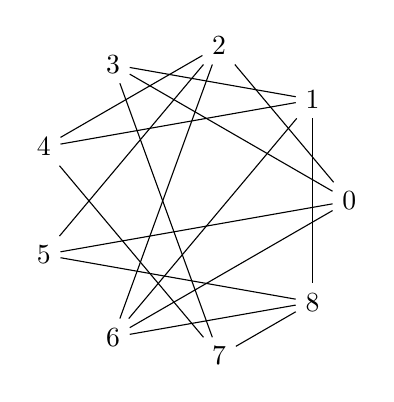
\begin{tikzpicture}
      \draw
        (0.0:2) node (0){0}
        (40.0:2) node (1){1}
        (80.0:2) node (2){2}
        (120.0:2) node (3){3}
        (160.0:2) node (4){4}
        (200.0:2) node (5){5}
        (240.0:2) node (6){6}
        (280.0:2) node (7){7}
        (320.0:2) node (8){8};
      \begin{scope}[-]
        \draw (0) to (2);
        \draw (0) to (3);
        \draw (0) to (5);
        \draw (0) to (6);
        \draw (1) to (3);
        \draw (1) to (4);
        \draw (1) to (6);
        \draw (1) to (8);
        \draw (2) to (4);
        \draw (2) to (5);
        \draw (2) to (6);
        \draw (3) to (7);
        \draw (4) to (7);
        \draw (5) to (8);
        \draw (6) to (8);
        \draw (7) to (8);
      \end{scope}
    \end{tikzpicture}
\end{figure}
\begin{itemize}
\item signature: 011011000110101011100000100010001011
\item g: Graph with 9 nodes and 16 edges
\item order: 9
\item size: 16
\item max degree: 4
\item degrees: 3,3,3,3,4,4,4,4,4
\item is tree: 0
\item is bipartite: 0
\item has bridge: 0
\item is chordal: 0
\item is complete: 0
\item min cycle basis weight: 29
\item min cycle basis size: 8
\item diameter: 2
\item radius: 2
\item is eulerian: 0
\item is planar: 0
\item number of faces: 9
\item is regular: 0
\item p3: 33
\item p4: 41
\item property hash: 61ab8d73d531460c2a489fa7aa119c74815b3f8593b94a0cd15b63958b8eae22
\end{itemize}
\newpage
\begin{figure}
  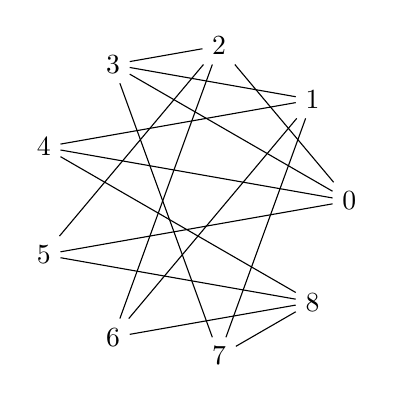
\begin{tikzpicture}
      \draw
        (0.0:2) node (0){0}
        (40.0:2) node (1){1}
        (80.0:2) node (2){2}
        (120.0:2) node (3){3}
        (160.0:2) node (4){4}
        (200.0:2) node (5){5}
        (240.0:2) node (6){6}
        (280.0:2) node (7){7}
        (320.0:2) node (8){8};
      \begin{scope}[-]
        \draw (0) to (2);
        \draw (0) to (3);
        \draw (0) to (4);
        \draw (0) to (5);
        \draw (1) to (3);
        \draw (1) to (4);
        \draw (1) to (6);
        \draw (1) to (7);
        \draw (2) to (3);
        \draw (2) to (5);
        \draw (2) to (6);
        \draw (3) to (7);
        \draw (4) to (8);
        \draw (5) to (8);
        \draw (6) to (8);
        \draw (7) to (8);
      \end{scope}
    \end{tikzpicture}
\end{figure}
\begin{itemize}
\item signature: 011110000110110101100000100001001011
\item g: Graph with 9 nodes and 16 edges
\item order: 9
\item size: 16
\item max degree: 4
\item degrees: 3,3,3,3,4,4,4,4,4
\item is tree: 0
\item is bipartite: 0
\item has bridge: 0
\item is chordal: 0
\item is complete: 0
\item min cycle basis weight: 29
\item min cycle basis size: 8
\item diameter: 3
\item radius: 2
\item is eulerian: 0
\item is planar: 0
\item number of faces: 9
\item is regular: 0
\item p3: 33
\item p4: 41
\item property hash: 4370a8655b5c3845b27f4a4c30cc67a85c3a40833a104c3d028b585c09d9b1c1
\end{itemize}
\newpage
\begin{figure}
  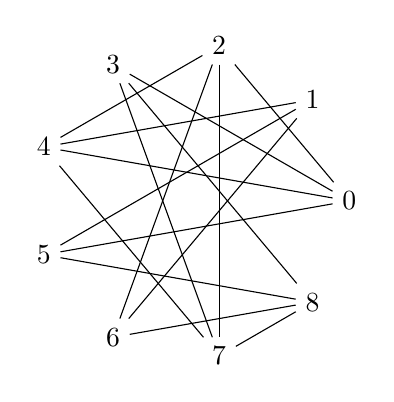
\begin{tikzpicture}
      \draw
        (0.0:2) node (0){0}
        (40.0:2) node (1){1}
        (80.0:2) node (2){2}
        (120.0:2) node (3){3}
        (160.0:2) node (4){4}
        (200.0:2) node (5){5}
        (240.0:2) node (6){6}
        (280.0:2) node (7){7}
        (320.0:2) node (8){8};
      \begin{scope}[-]
        \draw (0) to (2);
        \draw (0) to (3);
        \draw (0) to (4);
        \draw (0) to (5);
        \draw (1) to (4);
        \draw (1) to (5);
        \draw (1) to (6);
        \draw (2) to (4);
        \draw (2) to (6);
        \draw (2) to (7);
        \draw (3) to (7);
        \draw (3) to (8);
        \draw (4) to (7);
        \draw (5) to (8);
        \draw (6) to (8);
        \draw (7) to (8);
      \end{scope}
    \end{tikzpicture}
\end{figure}
\begin{itemize}
\item signature: 011110000011100010110000110010001011
\item g: Graph with 9 nodes and 16 edges
\item order: 9
\item size: 16
\item max degree: 4
\item degrees: 3,3,3,3,4,4,4,4,4
\item is tree: 0
\item is bipartite: 0
\item has bridge: 0
\item is chordal: 0
\item is complete: 0
\item min cycle basis weight: 29
\item min cycle basis size: 8
\item diameter: 3
\item radius: 2
\item is eulerian: 0
\item is planar: 0
\item number of faces: 9
\item is regular: 0
\item p3: 33
\item p4: 41
\item property hash: 4370a8655b5c3845b27f4a4c30cc67a85c3a40833a104c3d028b585c09d9b1c1
\end{itemize}
\newpage
\begin{figure}
  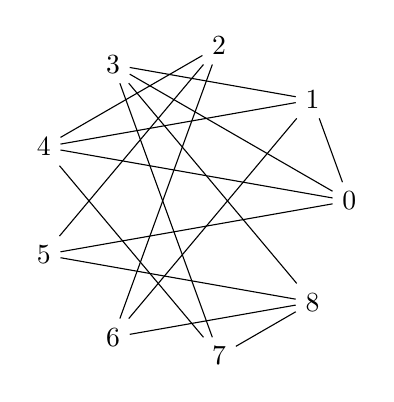
\begin{tikzpicture}
      \draw
        (0.0:2) node (0){0}
        (40.0:2) node (1){1}
        (80.0:2) node (2){2}
        (120.0:2) node (3){3}
        (160.0:2) node (4){4}
        (200.0:2) node (5){5}
        (240.0:2) node (6){6}
        (280.0:2) node (7){7}
        (320.0:2) node (8){8};
      \begin{scope}[-]
        \draw (0) to (1);
        \draw (0) to (3);
        \draw (0) to (4);
        \draw (0) to (5);
        \draw (1) to (3);
        \draw (1) to (4);
        \draw (1) to (6);
        \draw (2) to (4);
        \draw (2) to (5);
        \draw (2) to (6);
        \draw (3) to (7);
        \draw (3) to (8);
        \draw (4) to (7);
        \draw (5) to (8);
        \draw (6) to (8);
        \draw (7) to (8);
      \end{scope}
    \end{tikzpicture}
\end{figure}
\begin{itemize}
\item signature: 101110000110100011100000110010001011
\item g: Graph with 9 nodes and 16 edges
\item order: 9
\item size: 16
\item max degree: 4
\item degrees: 3,3,3,3,4,4,4,4,4
\item is tree: 0
\item is bipartite: 0
\item has bridge: 0
\item is chordal: 0
\item is complete: 0
\item min cycle basis weight: 29
\item min cycle basis size: 8
\item diameter: 3
\item radius: 2
\item is eulerian: 0
\item is planar: 0
\item number of faces: 9
\item is regular: 0
\item p3: 33
\item p4: 41
\item property hash: 4370a8655b5c3845b27f4a4c30cc67a85c3a40833a104c3d028b585c09d9b1c1
\end{itemize}
\newpage
\begin{figure}
  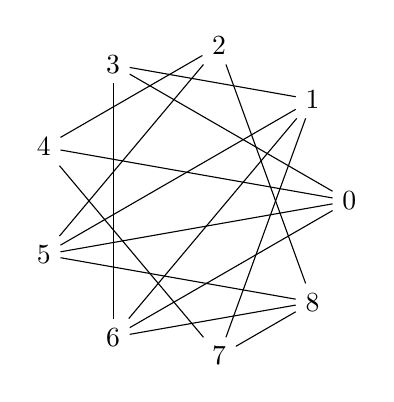
\begin{tikzpicture}
      \draw
        (0.0:2) node (0){0}
        (40.0:2) node (1){1}
        (80.0:2) node (2){2}
        (120.0:2) node (3){3}
        (160.0:2) node (4){4}
        (200.0:2) node (5){5}
        (240.0:2) node (6){6}
        (280.0:2) node (7){7}
        (320.0:2) node (8){8};
      \begin{scope}[-]
        \draw (0) to (3);
        \draw (0) to (4);
        \draw (0) to (5);
        \draw (0) to (6);
        \draw (1) to (3);
        \draw (1) to (5);
        \draw (1) to (6);
        \draw (1) to (7);
        \draw (2) to (4);
        \draw (2) to (5);
        \draw (2) to (8);
        \draw (3) to (6);
        \draw (4) to (7);
        \draw (5) to (8);
        \draw (6) to (8);
        \draw (7) to (8);
      \end{scope}
    \end{tikzpicture}
\end{figure}
\begin{itemize}
\item signature: 001111000101110011001001000010001011
\item g: Graph with 9 nodes and 16 edges
\item order: 9
\item size: 16
\item max degree: 4
\item degrees: 3,3,3,3,4,4,4,4,4
\item is tree: 0
\item is bipartite: 0
\item has bridge: 0
\item is chordal: 0
\item is complete: 0
\item min cycle basis weight: 29
\item min cycle basis size: 8
\item diameter: 3
\item radius: 2
\item is eulerian: 0
\item is planar: 0
\item number of faces: 9
\item is regular: 0
\item p3: 33
\item p4: 41
\item property hash: 4370a8655b5c3845b27f4a4c30cc67a85c3a40833a104c3d028b585c09d9b1c1
\end{itemize}
\newpage
\begin{figure}
  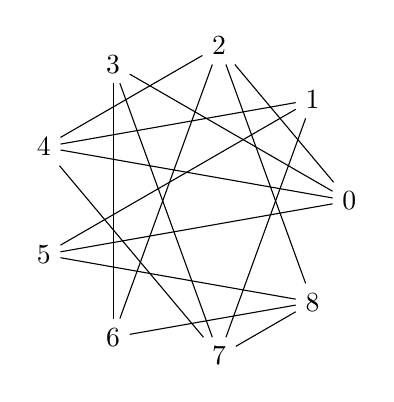
\begin{tikzpicture}
      \draw
        (0.0:2) node (0){0}
        (40.0:2) node (1){1}
        (80.0:2) node (2){2}
        (120.0:2) node (3){3}
        (160.0:2) node (4){4}
        (200.0:2) node (5){5}
        (240.0:2) node (6){6}
        (280.0:2) node (7){7}
        (320.0:2) node (8){8};
      \begin{scope}[-]
        \draw (0) to (2);
        \draw (0) to (3);
        \draw (0) to (4);
        \draw (0) to (5);
        \draw (1) to (4);
        \draw (1) to (5);
        \draw (1) to (7);
        \draw (2) to (4);
        \draw (2) to (6);
        \draw (2) to (8);
        \draw (3) to (6);
        \draw (3) to (7);
        \draw (4) to (7);
        \draw (5) to (8);
        \draw (6) to (8);
        \draw (7) to (8);
      \end{scope}
    \end{tikzpicture}
\end{figure}
\begin{itemize}
\item signature: 011110000011010010101001100010001011
\item g: Graph with 9 nodes and 16 edges
\item order: 9
\item size: 16
\item max degree: 4
\item degrees: 3,3,3,3,4,4,4,4,4
\item is tree: 0
\item is bipartite: 0
\item has bridge: 0
\item is chordal: 0
\item is complete: 0
\item min cycle basis weight: 29
\item min cycle basis size: 8
\item diameter: 3
\item radius: 2
\item is eulerian: 0
\item is planar: 0
\item number of faces: 9
\item is regular: 0
\item p3: 33
\item p4: 41
\item property hash: 4370a8655b5c3845b27f4a4c30cc67a85c3a40833a104c3d028b585c09d9b1c1
\end{itemize}
\newpage
\begin{figure}
  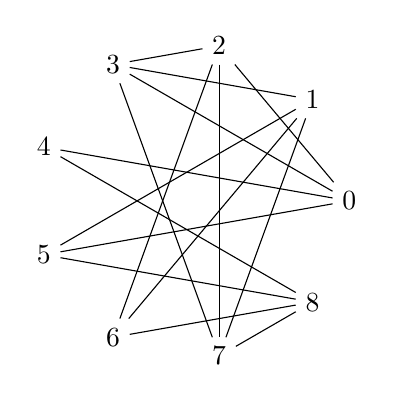
\begin{tikzpicture}
      \draw
        (0.0:2) node (0){0}
        (40.0:2) node (1){1}
        (80.0:2) node (2){2}
        (120.0:2) node (3){3}
        (160.0:2) node (4){4}
        (200.0:2) node (5){5}
        (240.0:2) node (6){6}
        (280.0:2) node (7){7}
        (320.0:2) node (8){8};
      \begin{scope}[-]
        \draw (0) to (2);
        \draw (0) to (3);
        \draw (0) to (4);
        \draw (0) to (5);
        \draw (1) to (3);
        \draw (1) to (5);
        \draw (1) to (6);
        \draw (1) to (7);
        \draw (2) to (3);
        \draw (2) to (6);
        \draw (2) to (7);
        \draw (3) to (7);
        \draw (4) to (8);
        \draw (5) to (8);
        \draw (6) to (8);
        \draw (7) to (8);
      \end{scope}
    \end{tikzpicture}
\end{figure}
\begin{itemize}
\item signature: 011110000101110100110000100001001011
\item g: Graph with 9 nodes and 16 edges
\item order: 9
\item size: 16
\item max degree: 4
\item degrees: 2,3,3,4,4,4,4,4,4
\item is tree: 0
\item is bipartite: 0
\item has bridge: 0
\item is chordal: 0
\item is complete: 0
\item min cycle basis weight: 29
\item min cycle basis size: 8
\item diameter: 3
\item radius: 2
\item is eulerian: 0
\item is planar: 0
\item number of faces: 9
\item is regular: 0
\item p3: 34
\item p4: 41
\item property hash: d234c5a161725cf58fd5f60a78439b6333f1002525986e9e4985f06fc59e75e1
\end{itemize}
\newpage
\begin{figure}
  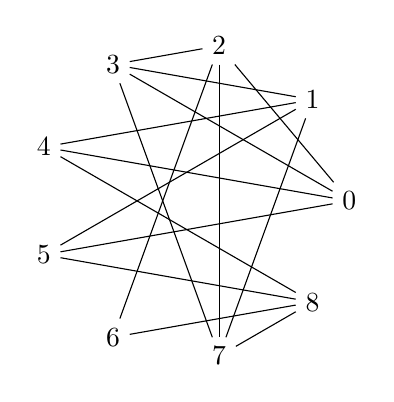
\begin{tikzpicture}
      \draw
        (0.0:2) node (0){0}
        (40.0:2) node (1){1}
        (80.0:2) node (2){2}
        (120.0:2) node (3){3}
        (160.0:2) node (4){4}
        (200.0:2) node (5){5}
        (240.0:2) node (6){6}
        (280.0:2) node (7){7}
        (320.0:2) node (8){8};
      \begin{scope}[-]
        \draw (0) to (2);
        \draw (0) to (3);
        \draw (0) to (4);
        \draw (0) to (5);
        \draw (1) to (3);
        \draw (1) to (4);
        \draw (1) to (5);
        \draw (1) to (7);
        \draw (2) to (3);
        \draw (2) to (6);
        \draw (2) to (7);
        \draw (3) to (7);
        \draw (4) to (8);
        \draw (5) to (8);
        \draw (6) to (8);
        \draw (7) to (8);
      \end{scope}
    \end{tikzpicture}
\end{figure}
\begin{itemize}
\item signature: 011110000111010100110000100001001011
\item g: Graph with 9 nodes and 16 edges
\item order: 9
\item size: 16
\item max degree: 4
\item degrees: 2,3,3,4,4,4,4,4,4
\item is tree: 0
\item is bipartite: 0
\item has bridge: 0
\item is chordal: 0
\item is complete: 0
\item min cycle basis weight: 29
\item min cycle basis size: 8
\item diameter: 3
\item radius: 2
\item is eulerian: 0
\item is planar: 0
\item number of faces: 9
\item is regular: 0
\item p3: 34
\item p4: 41
\item property hash: d234c5a161725cf58fd5f60a78439b6333f1002525986e9e4985f06fc59e75e1
\end{itemize}
\newpage
\begin{figure}
  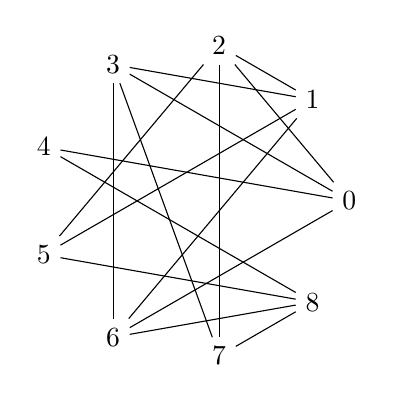
\begin{tikzpicture}
      \draw
        (0.0:2) node (0){0}
        (40.0:2) node (1){1}
        (80.0:2) node (2){2}
        (120.0:2) node (3){3}
        (160.0:2) node (4){4}
        (200.0:2) node (5){5}
        (240.0:2) node (6){6}
        (280.0:2) node (7){7}
        (320.0:2) node (8){8};
      \begin{scope}[-]
        \draw (0) to (2);
        \draw (0) to (3);
        \draw (0) to (4);
        \draw (0) to (6);
        \draw (1) to (2);
        \draw (1) to (3);
        \draw (1) to (5);
        \draw (1) to (6);
        \draw (2) to (5);
        \draw (2) to (7);
        \draw (3) to (6);
        \draw (3) to (7);
        \draw (4) to (8);
        \draw (5) to (8);
        \draw (6) to (8);
        \draw (7) to (8);
      \end{scope}
    \end{tikzpicture}
\end{figure}
\begin{itemize}
\item signature: 011101001101100001010001100001001011
\item g: Graph with 9 nodes and 16 edges
\item order: 9
\item size: 16
\item max degree: 4
\item degrees: 2,3,3,4,4,4,4,4,4
\item is tree: 0
\item is bipartite: 0
\item has bridge: 0
\item is chordal: 0
\item is complete: 0
\item min cycle basis weight: 29
\item min cycle basis size: 8
\item diameter: 3
\item radius: 2
\item is eulerian: 0
\item is planar: 0
\item number of faces: 9
\item is regular: 0
\item p3: 34
\item p4: 41
\item property hash: d234c5a161725cf58fd5f60a78439b6333f1002525986e9e4985f06fc59e75e1
\end{itemize}
\newpage
\begin{figure}
  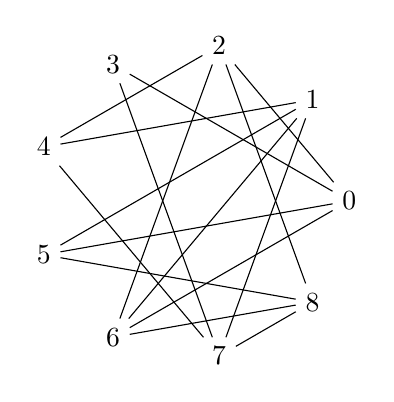
\begin{tikzpicture}
      \draw
        (0.0:2) node (0){0}
        (40.0:2) node (1){1}
        (80.0:2) node (2){2}
        (120.0:2) node (3){3}
        (160.0:2) node (4){4}
        (200.0:2) node (5){5}
        (240.0:2) node (6){6}
        (280.0:2) node (7){7}
        (320.0:2) node (8){8};
      \begin{scope}[-]
        \draw (0) to (2);
        \draw (0) to (3);
        \draw (0) to (5);
        \draw (0) to (6);
        \draw (1) to (4);
        \draw (1) to (5);
        \draw (1) to (6);
        \draw (1) to (7);
        \draw (2) to (4);
        \draw (2) to (6);
        \draw (2) to (8);
        \draw (3) to (7);
        \draw (4) to (7);
        \draw (5) to (8);
        \draw (6) to (8);
        \draw (7) to (8);
      \end{scope}
    \end{tikzpicture}
\end{figure}
\begin{itemize}
\item signature: 011011000011110010101000100010001011
\item g: Graph with 9 nodes and 16 edges
\item order: 9
\item size: 16
\item max degree: 4
\item degrees: 2,3,3,4,4,4,4,4,4
\item is tree: 0
\item is bipartite: 0
\item has bridge: 0
\item is chordal: 0
\item is complete: 0
\item min cycle basis weight: 30
\item min cycle basis size: 8
\item diameter: 2
\item radius: 2
\item is eulerian: 0
\item is planar: 0
\item number of faces: 9
\item is regular: 0
\item p3: 34
\item p4: 41
\item property hash: 47d746e6af344fe780a99e9942532ee5a46f70fadf2b2b9961af198863b846a5
\end{itemize}
\newpage
\begin{figure}
  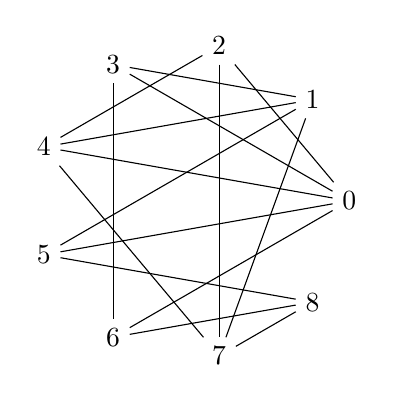
\begin{tikzpicture}
      \draw
        (0.0:2) node (0){0}
        (40.0:2) node (1){1}
        (80.0:2) node (2){2}
        (120.0:2) node (3){3}
        (160.0:2) node (4){4}
        (200.0:2) node (5){5}
        (240.0:2) node (6){6}
        (280.0:2) node (7){7}
        (320.0:2) node (8){8};
      \begin{scope}[-]
        \draw (0) to (2);
        \draw (0) to (3);
        \draw (0) to (4);
        \draw (0) to (5);
        \draw (0) to (6);
        \draw (1) to (3);
        \draw (1) to (4);
        \draw (1) to (5);
        \draw (1) to (7);
        \draw (2) to (4);
        \draw (2) to (7);
        \draw (3) to (6);
        \draw (4) to (7);
        \draw (5) to (8);
        \draw (6) to (8);
        \draw (7) to (8);
      \end{scope}
    \end{tikzpicture}
\end{figure}
\begin{itemize}
\item signature: 011111000111010010010001000010001011
\item g: Graph with 9 nodes and 16 edges
\item order: 9
\item size: 16
\item max degree: 5
\item degrees: 3,3,3,3,3,4,4,4,5
\item is tree: 0
\item is bipartite: 0
\item has bridge: 0
\item is chordal: 0
\item is complete: 0
\item min cycle basis weight: 28
\item min cycle basis size: 8
\item diameter: 2
\item radius: 2
\item is eulerian: 0
\item is planar: 0
\item number of faces: 9
\item is regular: 0
\item p3: 31
\item p4: 41
\item property hash: 275fc0f9c22f299621b2da5ba6fba77391f8659604edcc9d05d02d67bfbece0a
\end{itemize}
\newpage
\begin{figure}
  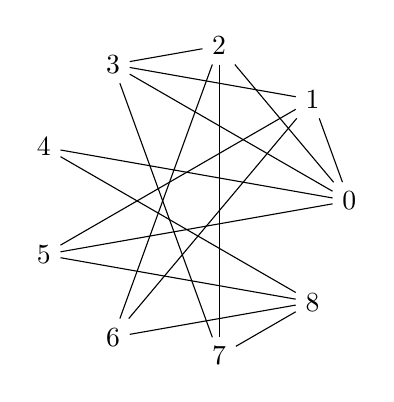
\begin{tikzpicture}
      \draw
        (0.0:2) node (0){0}
        (40.0:2) node (1){1}
        (80.0:2) node (2){2}
        (120.0:2) node (3){3}
        (160.0:2) node (4){4}
        (200.0:2) node (5){5}
        (240.0:2) node (6){6}
        (280.0:2) node (7){7}
        (320.0:2) node (8){8};
      \begin{scope}[-]
        \draw (0) to (1);
        \draw (0) to (2);
        \draw (0) to (3);
        \draw (0) to (4);
        \draw (0) to (5);
        \draw (1) to (3);
        \draw (1) to (5);
        \draw (1) to (6);
        \draw (2) to (3);
        \draw (2) to (6);
        \draw (2) to (7);
        \draw (3) to (7);
        \draw (4) to (8);
        \draw (5) to (8);
        \draw (6) to (8);
        \draw (7) to (8);
      \end{scope}
    \end{tikzpicture}
\end{figure}
\begin{itemize}
\item signature: 111110000101100100110000100001001011
\item g: Graph with 9 nodes and 16 edges
\item order: 9
\item size: 16
\item max degree: 5
\item degrees: 2,3,3,3,4,4,4,4,5
\item is tree: 0
\item is bipartite: 0
\item has bridge: 0
\item is chordal: 0
\item is complete: 0
\item min cycle basis weight: 28
\item min cycle basis size: 8
\item diameter: 2
\item radius: 2
\item is eulerian: 0
\item is planar: 0
\item number of faces: 9
\item is regular: 0
\item p3: 32
\item p4: 41
\item property hash: 71023aaf89cf8de1ea791bfaebe9d4a02bea5effeac9ccc8edb81f09fe9f0f3c
\end{itemize}
\newpage
\begin{figure}
  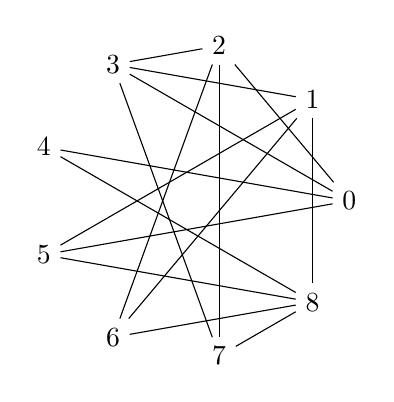
\begin{tikzpicture}
      \draw
        (0.0:2) node (0){0}
        (40.0:2) node (1){1}
        (80.0:2) node (2){2}
        (120.0:2) node (3){3}
        (160.0:2) node (4){4}
        (200.0:2) node (5){5}
        (240.0:2) node (6){6}
        (280.0:2) node (7){7}
        (320.0:2) node (8){8};
      \begin{scope}[-]
        \draw (0) to (2);
        \draw (0) to (3);
        \draw (0) to (4);
        \draw (0) to (5);
        \draw (1) to (3);
        \draw (1) to (5);
        \draw (1) to (6);
        \draw (1) to (8);
        \draw (2) to (3);
        \draw (2) to (6);
        \draw (2) to (7);
        \draw (3) to (7);
        \draw (4) to (8);
        \draw (5) to (8);
        \draw (6) to (8);
        \draw (7) to (8);
      \end{scope}
    \end{tikzpicture}
\end{figure}
\begin{itemize}
\item signature: 011110000101101100110000100001001011
\item g: Graph with 9 nodes and 16 edges
\item order: 9
\item size: 16
\item max degree: 5
\item degrees: 2,3,3,3,4,4,4,4,5
\item is tree: 0
\item is bipartite: 0
\item has bridge: 0
\item is chordal: 0
\item is complete: 0
\item min cycle basis weight: 28
\item min cycle basis size: 8
\item diameter: 2
\item radius: 2
\item is eulerian: 0
\item is planar: 0
\item number of faces: 9
\item is regular: 0
\item p3: 32
\item p4: 41
\item property hash: 71023aaf89cf8de1ea791bfaebe9d4a02bea5effeac9ccc8edb81f09fe9f0f3c
\end{itemize}
\newpage
\begin{figure}
  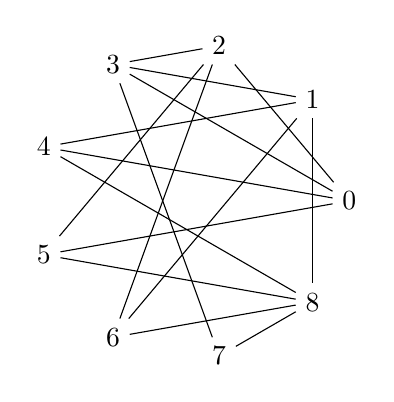
\begin{tikzpicture}
      \draw
        (0.0:2) node (0){0}
        (40.0:2) node (1){1}
        (80.0:2) node (2){2}
        (120.0:2) node (3){3}
        (160.0:2) node (4){4}
        (200.0:2) node (5){5}
        (240.0:2) node (6){6}
        (280.0:2) node (7){7}
        (320.0:2) node (8){8};
      \begin{scope}[-]
        \draw (0) to (2);
        \draw (0) to (3);
        \draw (0) to (4);
        \draw (0) to (5);
        \draw (1) to (3);
        \draw (1) to (4);
        \draw (1) to (6);
        \draw (1) to (8);
        \draw (2) to (3);
        \draw (2) to (5);
        \draw (2) to (6);
        \draw (3) to (7);
        \draw (4) to (8);
        \draw (5) to (8);
        \draw (6) to (8);
        \draw (7) to (8);
      \end{scope}
    \end{tikzpicture}
\end{figure}
\begin{itemize}
\item signature: 011110000110101101100000100001001011
\item g: Graph with 9 nodes and 16 edges
\item order: 9
\item size: 16
\item max degree: 5
\item degrees: 2,3,3,3,4,4,4,4,5
\item is tree: 0
\item is bipartite: 0
\item has bridge: 0
\item is chordal: 0
\item is complete: 0
\item min cycle basis weight: 28
\item min cycle basis size: 8
\item diameter: 2
\item radius: 2
\item is eulerian: 0
\item is planar: 0
\item number of faces: 9
\item is regular: 0
\item p3: 32
\item p4: 41
\item property hash: 71023aaf89cf8de1ea791bfaebe9d4a02bea5effeac9ccc8edb81f09fe9f0f3c
\end{itemize}
\newpage
\begin{figure}
  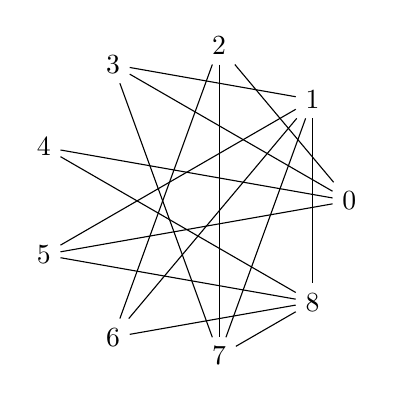
\begin{tikzpicture}
      \draw
        (0.0:2) node (0){0}
        (40.0:2) node (1){1}
        (80.0:2) node (2){2}
        (120.0:2) node (3){3}
        (160.0:2) node (4){4}
        (200.0:2) node (5){5}
        (240.0:2) node (6){6}
        (280.0:2) node (7){7}
        (320.0:2) node (8){8};
      \begin{scope}[-]
        \draw (0) to (2);
        \draw (0) to (3);
        \draw (0) to (4);
        \draw (0) to (5);
        \draw (1) to (3);
        \draw (1) to (5);
        \draw (1) to (6);
        \draw (1) to (7);
        \draw (1) to (8);
        \draw (2) to (6);
        \draw (2) to (7);
        \draw (3) to (7);
        \draw (4) to (8);
        \draw (5) to (8);
        \draw (6) to (8);
        \draw (7) to (8);
      \end{scope}
    \end{tikzpicture}
\end{figure}
\begin{itemize}
\item signature: 011110000101111000110000100001001011
\item g: Graph with 9 nodes and 16 edges
\item order: 9
\item size: 16
\item max degree: 5
\item degrees: 2,3,3,3,3,4,4,5,5
\item is tree: 0
\item is bipartite: 0
\item has bridge: 0
\item is chordal: 0
\item is complete: 0
\item min cycle basis weight: 28
\item min cycle basis size: 8
\item diameter: 2
\item radius: 2
\item is eulerian: 0
\item is planar: 0
\item number of faces: 9
\item is regular: 0
\item p3: 33
\item p4: 41
\item property hash: 79f399544fc2ee30598bf7764c00c109bdde0e409adde0a3fb73b2e19ee9e98d
\end{itemize}
\newpage
\begin{figure}
  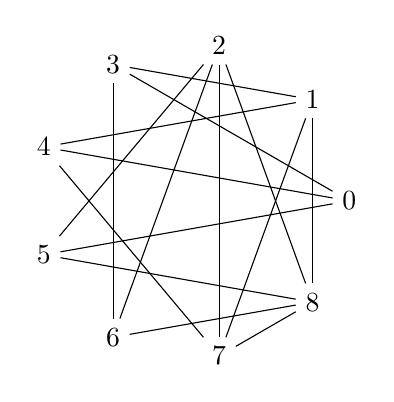
\begin{tikzpicture}
      \draw
        (0.0:2) node (0){0}
        (40.0:2) node (1){1}
        (80.0:2) node (2){2}
        (120.0:2) node (3){3}
        (160.0:2) node (4){4}
        (200.0:2) node (5){5}
        (240.0:2) node (6){6}
        (280.0:2) node (7){7}
        (320.0:2) node (8){8};
      \begin{scope}[-]
        \draw (0) to (3);
        \draw (0) to (4);
        \draw (0) to (5);
        \draw (1) to (3);
        \draw (1) to (4);
        \draw (1) to (7);
        \draw (1) to (8);
        \draw (2) to (5);
        \draw (2) to (6);
        \draw (2) to (7);
        \draw (2) to (8);
        \draw (3) to (6);
        \draw (4) to (7);
        \draw (5) to (8);
        \draw (6) to (8);
        \draw (7) to (8);
      \end{scope}
    \end{tikzpicture}
\end{figure}
\begin{itemize}
\item signature: 001110000110011001111001000010001011
\item g: Graph with 9 nodes and 16 edges
\item order: 9
\item size: 16
\item max degree: 5
\item degrees: 3,3,3,3,3,4,4,4,5
\item is tree: 0
\item is bipartite: 0
\item has bridge: 0
\item is chordal: 0
\item is complete: 0
\item min cycle basis weight: 28
\item min cycle basis size: 8
\item diameter: 3
\item radius: 2
\item is eulerian: 0
\item is planar: 0
\item number of faces: 9
\item is regular: 0
\item p3: 28
\item p4: 41
\item property hash: f86cbbb692336acdd2c75770e3d300abb269024bbd56f8f2449d4bf49a06df05
\end{itemize}
\newpage
\begin{figure}
  \begin{tikzpicture}
      \draw
        (0.0:2) node (0){0}
        (40.0:2) node (1){1}
        (80.0:2) node (2){2}
        (120.0:2) node (3){3}
        (160.0:2) node (4){4}
        (200.0:2) node (5){5}
        (240.0:2) node (6){6}
        (280.0:2) node (7){7}
        (320.0:2) node (8){8};
      \begin{scope}[-]
        \draw (0) to (2);
        \draw (0) to (3);
        \draw (0) to (4);
        \draw (0) to (5);
        \draw (1) to (4);
        \draw (1) to (6);
        \draw (1) to (7);
        \draw (1) to (8);
        \draw (2) to (5);
        \draw (2) to (7);
        \draw (3) to (6);
        \draw (3) to (7);
        \draw (4) to (8);
        \draw (5) to (8);
        \draw (6) to (8);
        \draw (7) to (8);
      \end{scope}
    \end{tikzpicture}
\end{figure}
\begin{itemize}
\item signature: 011110000010111001010001100001001011
\item g: Graph with 9 nodes and 16 edges
\item order: 9
\item size: 16
\item max degree: 5
\item degrees: 3,3,3,3,3,4,4,4,5
\item is tree: 0
\item is bipartite: 0
\item has bridge: 0
\item is chordal: 0
\item is complete: 0
\item min cycle basis weight: 28
\item min cycle basis size: 8
\item diameter: 3
\item radius: 2
\item is eulerian: 0
\item is planar: 0
\item number of faces: 9
\item is regular: 0
\item p3: 31
\item p4: 41
\item property hash: 5f0e30e18f90621dec54ce6133a70679aa125c9b991df6830cce591a175f4ac9
\end{itemize}
\newpage
\begin{figure}
  \begin{tikzpicture}
      \draw
        (0.0:2) node (0){0}
        (40.0:2) node (1){1}
        (80.0:2) node (2){2}
        (120.0:2) node (3){3}
        (160.0:2) node (4){4}
        (200.0:2) node (5){5}
        (240.0:2) node (6){6}
        (280.0:2) node (7){7}
        (320.0:2) node (8){8};
      \begin{scope}[-]
        \draw (0) to (2);
        \draw (0) to (3);
        \draw (0) to (4);
        \draw (0) to (6);
        \draw (1) to (3);
        \draw (1) to (4);
        \draw (1) to (5);
        \draw (1) to (8);
        \draw (2) to (5);
        \draw (2) to (7);
        \draw (2) to (8);
        \draw (3) to (6);
        \draw (4) to (7);
        \draw (5) to (8);
        \draw (6) to (8);
        \draw (7) to (8);
      \end{scope}
    \end{tikzpicture}
\end{figure}
\begin{itemize}
\item signature: 011101000111001001011001000010001011
\item g: Graph with 9 nodes and 16 edges
\item order: 9
\item size: 16
\item max degree: 5
\item degrees: 3,3,3,3,3,4,4,4,5
\item is tree: 0
\item is bipartite: 0
\item has bridge: 0
\item is chordal: 0
\item is complete: 0
\item min cycle basis weight: 28
\item min cycle basis size: 8
\item diameter: 3
\item radius: 2
\item is eulerian: 0
\item is planar: 0
\item number of faces: 9
\item is regular: 0
\item p3: 31
\item p4: 41
\item property hash: 5f0e30e18f90621dec54ce6133a70679aa125c9b991df6830cce591a175f4ac9
\end{itemize}
\newpage
\begin{figure}
  \begin{tikzpicture}
      \draw
        (0.0:2) node (0){0}
        (40.0:2) node (1){1}
        (80.0:2) node (2){2}
        (120.0:2) node (3){3}
        (160.0:2) node (4){4}
        (200.0:2) node (5){5}
        (240.0:2) node (6){6}
        (280.0:2) node (7){7}
        (320.0:2) node (8){8};
      \begin{scope}[-]
        \draw (0) to (1);
        \draw (0) to (2);
        \draw (0) to (3);
        \draw (0) to (5);
        \draw (0) to (6);
        \draw (1) to (3);
        \draw (1) to (4);
        \draw (1) to (5);
        \draw (2) to (5);
        \draw (2) to (7);
        \draw (3) to (6);
        \draw (3) to (7);
        \draw (4) to (8);
        \draw (5) to (8);
        \draw (6) to (8);
        \draw (7) to (8);
      \end{scope}
    \end{tikzpicture}
\end{figure}
\begin{itemize}
\item signature: 111011000111000001010001100001001011
\item g: Graph with 9 nodes and 16 edges
\item order: 9
\item size: 16
\item max degree: 5
\item degrees: 2,3,3,3,4,4,4,4,5
\item is tree: 0
\item is bipartite: 0
\item has bridge: 0
\item is chordal: 0
\item is complete: 0
\item min cycle basis weight: 28
\item min cycle basis size: 8
\item diameter: 3
\item radius: 2
\item is eulerian: 0
\item is planar: 0
\item number of faces: 9
\item is regular: 0
\item p3: 32
\item p4: 41
\item property hash: 7d1c71b38e27ccaf07fe1256375ed2b6e3a5cf01a860163f01a66057c768b7ee
\end{itemize}
\newpage
\begin{figure}
  \begin{tikzpicture}
      \draw
        (0.0:2) node (0){0}
        (40.0:2) node (1){1}
        (80.0:2) node (2){2}
        (120.0:2) node (3){3}
        (160.0:2) node (4){4}
        (200.0:2) node (5){5}
        (240.0:2) node (6){6}
        (280.0:2) node (7){7}
        (320.0:2) node (8){8};
      \begin{scope}[-]
        \draw (0) to (2);
        \draw (0) to (3);
        \draw (0) to (4);
        \draw (0) to (5);
        \draw (1) to (3);
        \draw (1) to (4);
        \draw (1) to (6);
        \draw (1) to (8);
        \draw (2) to (5);
        \draw (2) to (6);
        \draw (2) to (8);
        \draw (3) to (7);
        \draw (4) to (7);
        \draw (5) to (8);
        \draw (6) to (8);
        \draw (7) to (8);
      \end{scope}
    \end{tikzpicture}
\end{figure}
\begin{itemize}
\item signature: 011110000110101001101000100010001011
\item g: Graph with 9 nodes and 16 edges
\item order: 9
\item size: 16
\item max degree: 5
\item degrees: 3,3,3,3,3,4,4,4,5
\item is tree: 0
\item is bipartite: 0
\item has bridge: 0
\item is chordal: 0
\item is complete: 0
\item min cycle basis weight: 29
\item min cycle basis size: 8
\item diameter: 2
\item radius: 2
\item is eulerian: 0
\item is planar: 0
\item number of faces: 9
\item is regular: 0
\item p3: 31
\item p4: 41
\item property hash: 5ef98a187956ad8ed6632c63ec1bc0359243294cd15143908f6a669947f5c7b9
\end{itemize}
\newpage
\begin{figure}
  \begin{tikzpicture}
      \draw
        (0.0:2) node (0){0}
        (40.0:2) node (1){1}
        (80.0:2) node (2){2}
        (120.0:2) node (3){3}
        (160.0:2) node (4){4}
        (200.0:2) node (5){5}
        (240.0:2) node (6){6}
        (280.0:2) node (7){7}
        (320.0:2) node (8){8};
      \begin{scope}[-]
        \draw (0) to (3);
        \draw (0) to (4);
        \draw (0) to (5);
        \draw (0) to (7);
        \draw (1) to (3);
        \draw (1) to (5);
        \draw (1) to (7);
        \draw (2) to (4);
        \draw (2) to (6);
        \draw (2) to (7);
        \draw (2) to (8);
        \draw (3) to (6);
        \draw (4) to (7);
        \draw (5) to (8);
        \draw (6) to (8);
        \draw (7) to (8);
      \end{scope}
    \end{tikzpicture}
\end{figure}
\begin{itemize}
\item signature: 001110100101010010111001000010001011
\item g: Graph with 9 nodes and 16 edges
\item order: 9
\item size: 16
\item max degree: 5
\item degrees: 3,3,3,3,3,4,4,4,5
\item is tree: 0
\item is bipartite: 0
\item has bridge: 0
\item is chordal: 0
\item is complete: 0
\item min cycle basis weight: 29
\item min cycle basis size: 8
\item diameter: 2
\item radius: 2
\item is eulerian: 0
\item is planar: 0
\item number of faces: 9
\item is regular: 0
\item p3: 31
\item p4: 41
\item property hash: 5ef98a187956ad8ed6632c63ec1bc0359243294cd15143908f6a669947f5c7b9
\end{itemize}
\newpage
\begin{figure}
  \begin{tikzpicture}
      \draw
        (0.0:2) node (0){0}
        (40.0:2) node (1){1}
        (80.0:2) node (2){2}
        (120.0:2) node (3){3}
        (160.0:2) node (4){4}
        (200.0:2) node (5){5}
        (240.0:2) node (6){6}
        (280.0:2) node (7){7}
        (320.0:2) node (8){8};
      \begin{scope}[-]
        \draw (0) to (1);
        \draw (0) to (2);
        \draw (0) to (3);
        \draw (0) to (4);
        \draw (0) to (6);
        \draw (1) to (3);
        \draw (1) to (5);
        \draw (1) to (6);
        \draw (2) to (5);
        \draw (2) to (7);
        \draw (3) to (6);
        \draw (3) to (7);
        \draw (4) to (8);
        \draw (5) to (8);
        \draw (6) to (8);
        \draw (7) to (8);
      \end{scope}
    \end{tikzpicture}
\end{figure}
\begin{itemize}
\item signature: 111101000101100001010001100001001011
\item g: Graph with 9 nodes and 16 edges
\item order: 9
\item size: 16
\item max degree: 5
\item degrees: 2,3,3,3,4,4,4,4,5
\item is tree: 0
\item is bipartite: 0
\item has bridge: 0
\item is chordal: 0
\item is complete: 0
\item min cycle basis weight: 29
\item min cycle basis size: 8
\item diameter: 2
\item radius: 2
\item is eulerian: 0
\item is planar: 0
\item number of faces: 9
\item is regular: 0
\item p3: 32
\item p4: 41
\item property hash: e5835b3b4d75637ac81b964d51693784cdd87c5e44120062f942efe60d4a0e04
\end{itemize}
\newpage
\begin{figure}
  \begin{tikzpicture}
      \draw
        (0.0:2) node (0){0}
        (40.0:2) node (1){1}
        (80.0:2) node (2){2}
        (120.0:2) node (3){3}
        (160.0:2) node (4){4}
        (200.0:2) node (5){5}
        (240.0:2) node (6){6}
        (280.0:2) node (7){7}
        (320.0:2) node (8){8};
      \begin{scope}[-]
        \draw (0) to (1);
        \draw (0) to (2);
        \draw (0) to (3);
        \draw (0) to (4);
        \draw (0) to (5);
        \draw (1) to (3);
        \draw (1) to (4);
        \draw (1) to (6);
        \draw (2) to (5);
        \draw (2) to (6);
        \draw (2) to (7);
        \draw (3) to (7);
        \draw (4) to (8);
        \draw (5) to (8);
        \draw (6) to (8);
        \draw (7) to (8);
      \end{scope}
    \end{tikzpicture}
\end{figure}
\begin{itemize}
\item signature: 111110000110100001110000100001001011
\item g: Graph with 9 nodes and 16 edges
\item order: 9
\item size: 16
\item max degree: 5
\item degrees: 3,3,3,3,3,4,4,4,5
\item is tree: 0
\item is bipartite: 0
\item has bridge: 0
\item is chordal: 0
\item is complete: 0
\item min cycle basis weight: 29
\item min cycle basis size: 8
\item diameter: 2
\item radius: 2
\item is eulerian: 0
\item is planar: 0
\item number of faces: 9
\item is regular: 0
\item p3: 34
\item p4: 41
\item property hash: 3687ce084e61480e2befc321b144f6a46cebe874f7eb00521b4af803a80f61eb
\end{itemize}
\newpage
\begin{figure}
  \begin{tikzpicture}
      \draw
        (0.0:2) node (0){0}
        (40.0:2) node (1){1}
        (80.0:2) node (2){2}
        (120.0:2) node (3){3}
        (160.0:2) node (4){4}
        (200.0:2) node (5){5}
        (240.0:2) node (6){6}
        (280.0:2) node (7){7}
        (320.0:2) node (8){8};
      \begin{scope}[-]
        \draw (0) to (1);
        \draw (0) to (3);
        \draw (0) to (4);
        \draw (0) to (5);
        \draw (1) to (4);
        \draw (1) to (6);
        \draw (1) to (7);
        \draw (2) to (5);
        \draw (2) to (7);
        \draw (2) to (8);
        \draw (3) to (6);
        \draw (3) to (7);
        \draw (4) to (8);
        \draw (5) to (8);
        \draw (6) to (8);
        \draw (7) to (8);
      \end{scope}
    \end{tikzpicture}
\end{figure}
\begin{itemize}
\item signature: 101110000010110001011001100001001011
\item g: Graph with 9 nodes and 16 edges
\item order: 9
\item size: 16
\item max degree: 5
\item degrees: 3,3,3,3,3,4,4,4,5
\item is tree: 0
\item is bipartite: 0
\item has bridge: 0
\item is chordal: 0
\item is complete: 0
\item min cycle basis weight: 29
\item min cycle basis size: 8
\item diameter: 2
\item radius: 2
\item is eulerian: 0
\item is planar: 0
\item number of faces: 9
\item is regular: 0
\item p3: 34
\item p4: 41
\item property hash: 3687ce084e61480e2befc321b144f6a46cebe874f7eb00521b4af803a80f61eb
\end{itemize}
\newpage
\begin{figure}
  \begin{tikzpicture}
      \draw
        (0.0:2) node (0){0}
        (40.0:2) node (1){1}
        (80.0:2) node (2){2}
        (120.0:2) node (3){3}
        (160.0:2) node (4){4}
        (200.0:2) node (5){5}
        (240.0:2) node (6){6}
        (280.0:2) node (7){7}
        (320.0:2) node (8){8};
      \begin{scope}[-]
        \draw (0) to (2);
        \draw (0) to (3);
        \draw (0) to (4);
        \draw (0) to (5);
        \draw (0) to (8);
        \draw (1) to (3);
        \draw (1) to (5);
        \draw (1) to (7);
        \draw (2) to (4);
        \draw (2) to (6);
        \draw (2) to (7);
        \draw (3) to (6);
        \draw (4) to (7);
        \draw (5) to (8);
        \draw (6) to (8);
        \draw (7) to (8);
      \end{scope}
    \end{tikzpicture}
\end{figure}
\begin{itemize}
\item signature: 011110010101010010110001000010001011
\item g: Graph with 9 nodes and 16 edges
\item order: 9
\item size: 16
\item max degree: 5
\item degrees: 3,3,3,3,3,4,4,4,5
\item is tree: 0
\item is bipartite: 0
\item has bridge: 0
\item is chordal: 0
\item is complete: 0
\item min cycle basis weight: 29
\item min cycle basis size: 8
\item diameter: 2
\item radius: 2
\item is eulerian: 0
\item is planar: 0
\item number of faces: 9
\item is regular: 0
\item p3: 34
\item p4: 41
\item property hash: 3687ce084e61480e2befc321b144f6a46cebe874f7eb00521b4af803a80f61eb
\end{itemize}
\newpage
\begin{figure}
  \begin{tikzpicture}
      \draw
        (0.0:2) node (0){0}
        (40.0:2) node (1){1}
        (80.0:2) node (2){2}
        (120.0:2) node (3){3}
        (160.0:2) node (4){4}
        (200.0:2) node (5){5}
        (240.0:2) node (6){6}
        (280.0:2) node (7){7}
        (320.0:2) node (8){8};
      \begin{scope}[-]
        \draw (0) to (2);
        \draw (0) to (3);
        \draw (0) to (4);
        \draw (0) to (7);
        \draw (0) to (8);
        \draw (1) to (3);
        \draw (1) to (4);
        \draw (1) to (5);
        \draw (1) to (6);
        \draw (2) to (5);
        \draw (2) to (6);
        \draw (3) to (7);
        \draw (4) to (8);
        \draw (5) to (8);
        \draw (6) to (8);
        \draw (7) to (8);
      \end{scope}
    \end{tikzpicture}
\end{figure}
\begin{itemize}
\item signature: 011100110111100001100000100001001011
\item g: Graph with 9 nodes and 16 edges
\item order: 9
\item size: 16
\item max degree: 5
\item degrees: 3,3,3,3,3,3,4,5,5
\item is tree: 0
\item is bipartite: 0
\item has bridge: 0
\item is chordal: 0
\item is complete: 0
\item min cycle basis weight: 29
\item min cycle basis size: 8
\item diameter: 2
\item radius: 2
\item is eulerian: 0
\item is planar: 0
\item number of faces: 9
\item is regular: 0
\item p3: 35
\item p4: 41
\item property hash: 6759563db7bb114b9ef7b08ae135415ba26649ad733a17b544c386c10518d507
\end{itemize}
\newpage
\begin{figure}
  \begin{tikzpicture}
      \draw
        (0.0:2) node (0){0}
        (40.0:2) node (1){1}
        (80.0:2) node (2){2}
        (120.0:2) node (3){3}
        (160.0:2) node (4){4}
        (200.0:2) node (5){5}
        (240.0:2) node (6){6}
        (280.0:2) node (7){7}
        (320.0:2) node (8){8};
      \begin{scope}[-]
        \draw (0) to (1);
        \draw (0) to (2);
        \draw (0) to (3);
        \draw (0) to (4);
        \draw (0) to (6);
        \draw (1) to (3);
        \draw (1) to (5);
        \draw (1) to (6);
        \draw (2) to (5);
        \draw (2) to (6);
        \draw (2) to (7);
        \draw (3) to (7);
        \draw (4) to (8);
        \draw (5) to (8);
        \draw (6) to (8);
        \draw (7) to (8);
      \end{scope}
    \end{tikzpicture}
\end{figure}
\begin{itemize}
\item signature: 111101000101100001110000100001001011
\item g: Graph with 9 nodes and 16 edges
\item order: 9
\item size: 16
\item max degree: 5
\item degrees: 2,3,3,3,4,4,4,4,5
\item is tree: 0
\item is bipartite: 0
\item has bridge: 0
\item is chordal: 0
\item is complete: 0
\item min cycle basis weight: 29
\item min cycle basis size: 8
\item diameter: 2
\item radius: 2
\item is eulerian: 0
\item is planar: 0
\item number of faces: 9
\item is regular: 0
\item p3: 35
\item p4: 41
\item property hash: b61c451dc2af001740db07457ba6b3e27d7ff7a30c0e3ac7e610f6165ac8744c
\end{itemize}
\newpage
\begin{figure}
  \begin{tikzpicture}
      \draw
        (0.0:2) node (0){0}
        (40.0:2) node (1){1}
        (80.0:2) node (2){2}
        (120.0:2) node (3){3}
        (160.0:2) node (4){4}
        (200.0:2) node (5){5}
        (240.0:2) node (6){6}
        (280.0:2) node (7){7}
        (320.0:2) node (8){8};
      \begin{scope}[-]
        \draw (0) to (2);
        \draw (0) to (3);
        \draw (0) to (4);
        \draw (0) to (6);
        \draw (0) to (8);
        \draw (1) to (3);
        \draw (1) to (4);
        \draw (1) to (5);
        \draw (2) to (5);
        \draw (2) to (7);
        \draw (3) to (6);
        \draw (3) to (7);
        \draw (4) to (8);
        \draw (5) to (8);
        \draw (6) to (8);
        \draw (7) to (8);
      \end{scope}
    \end{tikzpicture}
\end{figure}
\begin{itemize}
\item signature: 011101010111000001010001100001001011
\item g: Graph with 9 nodes and 16 edges
\item order: 9
\item size: 16
\item max degree: 5
\item degrees: 3,3,3,3,3,3,4,5,5
\item is tree: 0
\item is bipartite: 0
\item has bridge: 0
\item is chordal: 0
\item is complete: 0
\item min cycle basis weight: 29
\item min cycle basis size: 8
\item diameter: 2
\item radius: 2
\item is eulerian: 0
\item is planar: 0
\item number of faces: 9
\item is regular: 0
\item p3: 35
\item p4: 41
\item property hash: 6759563db7bb114b9ef7b08ae135415ba26649ad733a17b544c386c10518d507
\end{itemize}
\newpage
\begin{figure}
  \begin{tikzpicture}
      \draw
        (0.0:2) node (0){0}
        (40.0:2) node (1){1}
        (80.0:2) node (2){2}
        (120.0:2) node (3){3}
        (160.0:2) node (4){4}
        (200.0:2) node (5){5}
        (240.0:2) node (6){6}
        (280.0:2) node (7){7}
        (320.0:2) node (8){8};
      \begin{scope}[-]
        \draw (0) to (3);
        \draw (0) to (4);
        \draw (0) to (5);
        \draw (0) to (8);
        \draw (1) to (3);
        \draw (1) to (4);
        \draw (1) to (6);
        \draw (2) to (5);
        \draw (2) to (6);
        \draw (2) to (7);
        \draw (2) to (8);
        \draw (3) to (7);
        \draw (4) to (7);
        \draw (5) to (8);
        \draw (6) to (8);
        \draw (7) to (8);
      \end{scope}
    \end{tikzpicture}
\end{figure}
\begin{itemize}
\item signature: 001110010110100001111000100010001011
\item g: Graph with 9 nodes and 16 edges
\item order: 9
\item size: 16
\item max degree: 5
\item degrees: 3,3,3,3,3,4,4,4,5
\item is tree: 0
\item is bipartite: 0
\item has bridge: 0
\item is chordal: 0
\item is complete: 0
\item min cycle basis weight: 29
\item min cycle basis size: 8
\item diameter: 3
\item radius: 2
\item is eulerian: 0
\item is planar: 0
\item number of faces: 9
\item is regular: 0
\item p3: 31
\item p4: 41
\item property hash: 22a87f4da834bd757f30009c9e88c1baa516f7531b8cf74cfbe0e5ac80fb6022
\end{itemize}
\newpage
\begin{figure}
  \begin{tikzpicture}
      \draw
        (0.0:2) node (0){0}
        (40.0:2) node (1){1}
        (80.0:2) node (2){2}
        (120.0:2) node (3){3}
        (160.0:2) node (4){4}
        (200.0:2) node (5){5}
        (240.0:2) node (6){6}
        (280.0:2) node (7){7}
        (320.0:2) node (8){8};
      \begin{scope}[-]
        \draw (0) to (3);
        \draw (0) to (4);
        \draw (0) to (5);
        \draw (0) to (7);
        \draw (1) to (4);
        \draw (1) to (5);
        \draw (1) to (6);
        \draw (1) to (7);
        \draw (2) to (4);
        \draw (2) to (7);
        \draw (2) to (8);
        \draw (3) to (6);
        \draw (4) to (7);
        \draw (5) to (8);
        \draw (6) to (8);
        \draw (7) to (8);
      \end{scope}
    \end{tikzpicture}
\end{figure}
\begin{itemize}
\item signature: 001110100011110010011001000010001011
\item g: Graph with 9 nodes and 16 edges
\item order: 9
\item size: 16
\item max degree: 5
\item degrees: 2,3,3,3,4,4,4,4,5
\item is tree: 0
\item is bipartite: 0
\item has bridge: 0
\item is chordal: 0
\item is complete: 0
\item min cycle basis weight: 29
\item min cycle basis size: 8
\item diameter: 3
\item radius: 2
\item is eulerian: 0
\item is planar: 0
\item number of faces: 9
\item is regular: 0
\item p3: 32
\item p4: 41
\item property hash: 266c53748f50858b9321fb58ee82a2d624ad8e69944c66da3df7dda2f3e58ab5
\end{itemize}
\newpage
\begin{figure}
  \begin{tikzpicture}
      \draw
        (0.0:2) node (0){0}
        (40.0:2) node (1){1}
        (80.0:2) node (2){2}
        (120.0:2) node (3){3}
        (160.0:2) node (4){4}
        (200.0:2) node (5){5}
        (240.0:2) node (6){6}
        (280.0:2) node (7){7}
        (320.0:2) node (8){8};
      \begin{scope}[-]
        \draw (0) to (1);
        \draw (0) to (3);
        \draw (0) to (4);
        \draw (0) to (5);
        \draw (0) to (6);
        \draw (1) to (3);
        \draw (1) to (4);
        \draw (1) to (7);
        \draw (2) to (5);
        \draw (2) to (6);
        \draw (2) to (7);
        \draw (3) to (7);
        \draw (4) to (8);
        \draw (5) to (8);
        \draw (6) to (8);
        \draw (7) to (8);
      \end{scope}
    \end{tikzpicture}
\end{figure}
\begin{itemize}
\item signature: 101111000110010001110000100001001011
\item g: Graph with 9 nodes and 16 edges
\item order: 9
\item size: 16
\item max degree: 5
\item degrees: 3,3,3,3,3,4,4,4,5
\item is tree: 0
\item is bipartite: 0
\item has bridge: 0
\item is chordal: 0
\item is complete: 0
\item min cycle basis weight: 29
\item min cycle basis size: 8
\item diameter: 3
\item radius: 2
\item is eulerian: 0
\item is planar: 0
\item number of faces: 9
\item is regular: 0
\item p3: 34
\item p4: 41
\item property hash: b19bdc5402ee5d2f096f2c25effe0ea4490e672a94d5b94a40b80c920ee51a09
\end{itemize}
\newpage
\begin{figure}
  \begin{tikzpicture}
      \draw
        (0.0:2) node (0){0}
        (40.0:2) node (1){1}
        (80.0:2) node (2){2}
        (120.0:2) node (3){3}
        (160.0:2) node (4){4}
        (200.0:2) node (5){5}
        (240.0:2) node (6){6}
        (280.0:2) node (7){7}
        (320.0:2) node (8){8};
      \begin{scope}[-]
        \draw (0) to (2);
        \draw (0) to (3);
        \draw (0) to (4);
        \draw (0) to (5);
        \draw (1) to (4);
        \draw (1) to (6);
        \draw (1) to (7);
        \draw (2) to (5);
        \draw (2) to (7);
        \draw (2) to (8);
        \draw (3) to (6);
        \draw (3) to (7);
        \draw (4) to (8);
        \draw (5) to (8);
        \draw (6) to (8);
        \draw (7) to (8);
      \end{scope}
    \end{tikzpicture}
\end{figure}
\begin{itemize}
\item signature: 011110000010110001011001100001001011
\item g: Graph with 9 nodes and 16 edges
\item order: 9
\item size: 16
\item max degree: 5
\item degrees: 3,3,3,3,3,4,4,4,5
\item is tree: 0
\item is bipartite: 0
\item has bridge: 0
\item is chordal: 0
\item is complete: 0
\item min cycle basis weight: 29
\item min cycle basis size: 8
\item diameter: 3
\item radius: 2
\item is eulerian: 0
\item is planar: 0
\item number of faces: 9
\item is regular: 0
\item p3: 34
\item p4: 41
\item property hash: b19bdc5402ee5d2f096f2c25effe0ea4490e672a94d5b94a40b80c920ee51a09
\end{itemize}
\newpage
\begin{figure}
  \begin{tikzpicture}
      \draw
        (0.0:2) node (0){0}
        (40.0:2) node (1){1}
        (80.0:2) node (2){2}
        (120.0:2) node (3){3}
        (160.0:2) node (4){4}
        (200.0:2) node (5){5}
        (240.0:2) node (6){6}
        (280.0:2) node (7){7}
        (320.0:2) node (8){8};
      \begin{scope}[-]
        \draw (0) to (2);
        \draw (0) to (3);
        \draw (0) to (4);
        \draw (0) to (5);
        \draw (0) to (6);
        \draw (1) to (2);
        \draw (1) to (4);
        \draw (1) to (5);
        \draw (1) to (7);
        \draw (2) to (6);
        \draw (2) to (7);
        \draw (3) to (7);
        \draw (4) to (8);
        \draw (5) to (8);
        \draw (6) to (8);
        \draw (7) to (8);
      \end{scope}
    \end{tikzpicture}
\end{figure}
\begin{itemize}
\item signature: 011111001011010000110000100001001011
\item g: Graph with 9 nodes and 16 edges
\item order: 9
\item size: 16
\item max degree: 5
\item degrees: 2,3,3,3,4,4,4,4,5
\item is tree: 0
\item is bipartite: 0
\item has bridge: 0
\item is chordal: 0
\item is complete: 0
\item min cycle basis weight: 30
\item min cycle basis size: 8
\item diameter: 2
\item radius: 2
\item is eulerian: 0
\item is planar: 0
\item number of faces: 9
\item is regular: 0
\item p3: 38
\item p4: 41
\item property hash: 326071d2c187a624555cb259fa9aa74486349365fedc8c0aef82657b2c0b0a74
\end{itemize}
\newpage
\begin{figure}
  \begin{tikzpicture}
      \draw
        (0.0:2) node (0){0}
        (40.0:2) node (1){1}
        (80.0:2) node (2){2}
        (120.0:2) node (3){3}
        (160.0:2) node (4){4}
        (200.0:2) node (5){5}
        (240.0:2) node (6){6}
        (280.0:2) node (7){7}
        (320.0:2) node (8){8};
      \begin{scope}[-]
        \draw (0) to (1);
        \draw (0) to (3);
        \draw (0) to (4);
        \draw (0) to (5);
        \draw (0) to (6);
        \draw (1) to (3);
        \draw (1) to (4);
        \draw (1) to (6);
        \draw (2) to (5);
        \draw (2) to (6);
        \draw (2) to (7);
        \draw (3) to (7);
        \draw (4) to (8);
        \draw (5) to (8);
        \draw (6) to (8);
        \draw (7) to (8);
      \end{scope}
    \end{tikzpicture}
\end{figure}
\begin{itemize}
\item signature: 101111000110100001110000100001001011
\item g: Graph with 9 nodes and 16 edges
\item order: 9
\item size: 16
\item max degree: 5
\item degrees: 3,3,3,3,3,4,4,4,5
\item is tree: 0
\item is bipartite: 0
\item has bridge: 0
\item is chordal: 0
\item is complete: 0
\item min cycle basis weight: 30
\item min cycle basis size: 8
\item diameter: 3
\item radius: 2
\item is eulerian: 0
\item is planar: 0
\item number of faces: 9
\item is regular: 0
\item p3: 34
\item p4: 41
\item property hash: 916960d8797897134e15f26a474e2c66987bc137b3ce34e28ccdf2aae49306cc
\end{itemize}
\newpage
\begin{figure}
  \begin{tikzpicture}
      \draw
        (0.0:2) node (0){0}
        (40.0:2) node (1){1}
        (80.0:2) node (2){2}
        (120.0:2) node (3){3}
        (160.0:2) node (4){4}
        (200.0:2) node (5){5}
        (240.0:2) node (6){6}
        (280.0:2) node (7){7}
        (320.0:2) node (8){8};
      \begin{scope}[-]
        \draw (0) to (3);
        \draw (0) to (4);
        \draw (0) to (5);
        \draw (1) to (4);
        \draw (1) to (6);
        \draw (1) to (7);
        \draw (1) to (8);
        \draw (2) to (5);
        \draw (2) to (6);
        \draw (2) to (7);
        \draw (3) to (6);
        \draw (3) to (7);
        \draw (4) to (8);
        \draw (5) to (8);
        \draw (6) to (8);
        \draw (7) to (8);
      \end{scope}
    \end{tikzpicture}
\end{figure}
\begin{itemize}
\item signature: 001110000010111001110001100001001011
\item g: Graph with 9 nodes and 16 edges
\item order: 9
\item size: 16
\item max degree: 5
\item degrees: 3,3,3,3,3,4,4,4,5
\item is tree: 0
\item is bipartite: 0
\item has bridge: 0
\item is chordal: 0
\item is complete: 0
\item min cycle basis weight: 30
\item min cycle basis size: 8
\item diameter: 3
\item radius: 2
\item is eulerian: 0
\item is planar: 0
\item number of faces: 9
\item is regular: 0
\item p3: 34
\item p4: 41
\item property hash: 916960d8797897134e15f26a474e2c66987bc137b3ce34e28ccdf2aae49306cc
\end{itemize}
\newpage
\begin{figure}
  \begin{tikzpicture}
      \draw
        (0.0:2) node (0){0}
        (40.0:2) node (1){1}
        (80.0:2) node (2){2}
        (120.0:2) node (3){3}
        (160.0:2) node (4){4}
        (200.0:2) node (5){5}
        (240.0:2) node (6){6}
        (280.0:2) node (7){7}
        (320.0:2) node (8){8};
      \begin{scope}[-]
        \draw (0) to (3);
        \draw (0) to (4);
        \draw (0) to (5);
        \draw (1) to (4);
        \draw (1) to (5);
        \draw (1) to (7);
        \draw (1) to (8);
        \draw (2) to (5);
        \draw (2) to (6);
        \draw (2) to (7);
        \draw (3) to (6);
        \draw (3) to (7);
        \draw (4) to (8);
        \draw (5) to (8);
        \draw (6) to (8);
        \draw (7) to (8);
      \end{scope}
    \end{tikzpicture}
\end{figure}
\begin{itemize}
\item signature: 001110000011011001110001100001001011
\item g: Graph with 9 nodes and 16 edges
\item order: 9
\item size: 16
\item max degree: 5
\item degrees: 3,3,3,3,3,4,4,4,5
\item is tree: 0
\item is bipartite: 0
\item has bridge: 0
\item is chordal: 0
\item is complete: 0
\item min cycle basis weight: 30
\item min cycle basis size: 8
\item diameter: 3
\item radius: 2
\item is eulerian: 0
\item is planar: 0
\item number of faces: 9
\item is regular: 0
\item p3: 34
\item p4: 41
\item property hash: 916960d8797897134e15f26a474e2c66987bc137b3ce34e28ccdf2aae49306cc
\end{itemize}
\newpage
\begin{figure}
  \begin{tikzpicture}
      \draw
        (0.0:2) node (0){0}
        (40.0:2) node (1){1}
        (80.0:2) node (2){2}
        (120.0:2) node (3){3}
        (160.0:2) node (4){4}
        (200.0:2) node (5){5}
        (240.0:2) node (6){6}
        (280.0:2) node (7){7}
        (320.0:2) node (8){8};
      \begin{scope}[-]
        \draw (0) to (2);
        \draw (0) to (3);
        \draw (0) to (4);
        \draw (0) to (5);
        \draw (0) to (6);
        \draw (1) to (3);
        \draw (1) to (4);
        \draw (1) to (5);
        \draw (1) to (6);
        \draw (2) to (6);
        \draw (2) to (7);
        \draw (3) to (7);
        \draw (4) to (8);
        \draw (5) to (8);
        \draw (6) to (8);
        \draw (7) to (8);
      \end{scope}
    \end{tikzpicture}
\end{figure}
\begin{itemize}
\item signature: 011111000111100000110000100001001011
\item g: Graph with 9 nodes and 16 edges
\item order: 9
\item size: 16
\item max degree: 5
\item degrees: 3,3,3,3,3,4,4,4,5
\item is tree: 0
\item is bipartite: 0
\item has bridge: 0
\item is chordal: 0
\item is complete: 0
\item min cycle basis weight: 31
\item min cycle basis size: 8
\item diameter: 2
\item radius: 2
\item is eulerian: 0
\item is planar: 0
\item number of faces: 9
\item is regular: 0
\item p3: 40
\item p4: 41
\item property hash: 04416b7d9bfeb4b8a4b2617d403931086d86913fbc6bd297c955d911d2e9a3b6
\end{itemize}
\newpage
\begin{figure}
  \begin{tikzpicture}
      \draw
        (0.0:2) node (0){0}
        (40.0:2) node (1){1}
        (80.0:2) node (2){2}
        (120.0:2) node (3){3}
        (160.0:2) node (4){4}
        (200.0:2) node (5){5}
        (240.0:2) node (6){6}
        (280.0:2) node (7){7}
        (320.0:2) node (8){8};
      \begin{scope}[-]
        \draw (0) to (2);
        \draw (0) to (3);
        \draw (0) to (4);
        \draw (0) to (6);
        \draw (1) to (3);
        \draw (1) to (4);
        \draw (1) to (5);
        \draw (1) to (7);
        \draw (2) to (5);
        \draw (2) to (6);
        \draw (2) to (8);
        \draw (3) to (6);
        \draw (3) to (7);
        \draw (4) to (7);
        \draw (5) to (8);
        \draw (6) to (8);
        \draw (7) to (8);
      \end{scope}
    \end{tikzpicture}
\end{figure}
\begin{itemize}
\item signature: 011101000111010001101001100010001011
\item g: Graph with 9 nodes and 17 edges
\item order: 9
\item size: 17
\item max degree: 4
\item degrees: 3,3,4,4,4,4,4,4,4
\item is tree: 0
\item is bipartite: 0
\item has bridge: 0
\item is chordal: 0
\item is complete: 0
\item min cycle basis weight: 30
\item min cycle basis size: 9
\item diameter: 2
\item radius: 2
\item is eulerian: 0
\item is planar: 0
\item number of faces: 10
\item is regular: 0
\item p3: 30
\item p4: 41
\item property hash: 005ad0f85f5d4201baa08a2434def57be72bf1525c8b50d895655fb4b714d9b5
\end{itemize}
\newpage
\begin{figure}
  \begin{tikzpicture}
      \draw
        (0.0:2) node (0){0}
        (40.0:2) node (1){1}
        (80.0:2) node (2){2}
        (120.0:2) node (3){3}
        (160.0:2) node (4){4}
        (200.0:2) node (5){5}
        (240.0:2) node (6){6}
        (280.0:2) node (7){7}
        (320.0:2) node (8){8};
      \begin{scope}[-]
        \draw (0) to (1);
        \draw (0) to (3);
        \draw (0) to (4);
        \draw (0) to (5);
        \draw (1) to (3);
        \draw (1) to (5);
        \draw (1) to (6);
        \draw (2) to (4);
        \draw (2) to (6);
        \draw (2) to (7);
        \draw (2) to (8);
        \draw (3) to (6);
        \draw (3) to (7);
        \draw (4) to (7);
        \draw (5) to (8);
        \draw (6) to (8);
        \draw (7) to (8);
      \end{scope}
    \end{tikzpicture}
\end{figure}
\begin{itemize}
\item signature: 101110000101100010111001100010001011
\item g: Graph with 9 nodes and 17 edges
\item order: 9
\item size: 17
\item max degree: 4
\item degrees: 3,3,4,4,4,4,4,4,4
\item is tree: 0
\item is bipartite: 0
\item has bridge: 0
\item is chordal: 0
\item is complete: 0
\item min cycle basis weight: 30
\item min cycle basis size: 9
\item diameter: 2
\item radius: 2
\item is eulerian: 0
\item is planar: 0
\item number of faces: 10
\item is regular: 0
\item p3: 30
\item p4: 41
\item property hash: 005ad0f85f5d4201baa08a2434def57be72bf1525c8b50d895655fb4b714d9b5
\end{itemize}
\newpage
\begin{figure}
  \begin{tikzpicture}
      \draw
        (0.0:2) node (0){0}
        (40.0:2) node (1){1}
        (80.0:2) node (2){2}
        (120.0:2) node (3){3}
        (160.0:2) node (4){4}
        (200.0:2) node (5){5}
        (240.0:2) node (6){6}
        (280.0:2) node (7){7}
        (320.0:2) node (8){8};
      \begin{scope}[-]
        \draw (0) to (2);
        \draw (0) to (4);
        \draw (0) to (5);
        \draw (0) to (6);
        \draw (1) to (3);
        \draw (1) to (4);
        \draw (1) to (5);
        \draw (1) to (7);
        \draw (2) to (4);
        \draw (2) to (6);
        \draw (3) to (6);
        \draw (3) to (7);
        \draw (3) to (8);
        \draw (4) to (7);
        \draw (5) to (8);
        \draw (6) to (8);
        \draw (7) to (8);
      \end{scope}
    \end{tikzpicture}
\end{figure}
\begin{itemize}
\item signature: 010111000111010010100001110010001011
\item g: Graph with 9 nodes and 17 edges
\item order: 9
\item size: 17
\item max degree: 4
\item degrees: 3,3,4,4,4,4,4,4,4
\item is tree: 0
\item is bipartite: 0
\item has bridge: 0
\item is chordal: 0
\item is complete: 0
\item min cycle basis weight: 30
\item min cycle basis size: 9
\item diameter: 2
\item radius: 2
\item is eulerian: 0
\item is planar: 0
\item number of faces: 10
\item is regular: 0
\item p3: 30
\item p4: 41
\item property hash: 005ad0f85f5d4201baa08a2434def57be72bf1525c8b50d895655fb4b714d9b5
\end{itemize}
\newpage
\begin{figure}
  \begin{tikzpicture}
      \draw
        (0.0:2) node (0){0}
        (40.0:2) node (1){1}
        (80.0:2) node (2){2}
        (120.0:2) node (3){3}
        (160.0:2) node (4){4}
        (200.0:2) node (5){5}
        (240.0:2) node (6){6}
        (280.0:2) node (7){7}
        (320.0:2) node (8){8};
      \begin{scope}[-]
        \draw (0) to (1);
        \draw (0) to (3);
        \draw (0) to (4);
        \draw (0) to (6);
        \draw (1) to (4);
        \draw (1) to (5);
        \draw (1) to (6);
        \draw (2) to (4);
        \draw (2) to (5);
        \draw (2) to (7);
        \draw (2) to (8);
        \draw (3) to (6);
        \draw (3) to (7);
        \draw (4) to (7);
        \draw (5) to (8);
        \draw (6) to (8);
        \draw (7) to (8);
      \end{scope}
    \end{tikzpicture}
\end{figure}
\begin{itemize}
\item signature: 101101000011100011011001100010001011
\item g: Graph with 9 nodes and 17 edges
\item order: 9
\item size: 17
\item max degree: 4
\item degrees: 3,3,4,4,4,4,4,4,4
\item is tree: 0
\item is bipartite: 0
\item has bridge: 0
\item is chordal: 0
\item is complete: 0
\item min cycle basis weight: 30
\item min cycle basis size: 9
\item diameter: 3
\item radius: 2
\item is eulerian: 0
\item is planar: 1
\item number of faces: 10
\item is regular: 0
\item p3: 30
\item p4: 41
\item property hash: ab60c57588a57976dfee7e675ffaba0af64bba693d96acadaa85c1d7c61209d4
\end{itemize}
\newpage
\begin{figure}
  \begin{tikzpicture}
      \draw
        (0.0:2) node (0){0}
        (40.0:2) node (1){1}
        (80.0:2) node (2){2}
        (120.0:2) node (3){3}
        (160.0:2) node (4){4}
        (200.0:2) node (5){5}
        (240.0:2) node (6){6}
        (280.0:2) node (7){7}
        (320.0:2) node (8){8};
      \begin{scope}[-]
        \draw (0) to (2);
        \draw (0) to (3);
        \draw (0) to (4);
        \draw (0) to (6);
        \draw (1) to (3);
        \draw (1) to (4);
        \draw (1) to (5);
        \draw (1) to (7);
        \draw (2) to (4);
        \draw (2) to (6);
        \draw (2) to (7);
        \draw (3) to (6);
        \draw (3) to (8);
        \draw (4) to (7);
        \draw (5) to (8);
        \draw (6) to (8);
        \draw (7) to (8);
      \end{scope}
    \end{tikzpicture}
\end{figure}
\begin{itemize}
\item signature: 011101000111010010110001010010001011
\item g: Graph with 9 nodes and 17 edges
\item order: 9
\item size: 17
\item max degree: 4
\item degrees: 2,4,4,4,4,4,4,4,4
\item is tree: 0
\item is bipartite: 0
\item has bridge: 0
\item is chordal: 0
\item is complete: 0
\item min cycle basis weight: 30
\item min cycle basis size: 9
\item diameter: 3
\item radius: 2
\item is eulerian: 1
\item is planar: 1
\item number of faces: 10
\item is regular: 0
\item p3: 31
\item p4: 41
\item property hash: 05d162f209f01ce7af2827dc7de1876e8deca7d218b4190914d6e93dc1973695
\end{itemize}
\newpage
\begin{figure}
  \begin{tikzpicture}
      \draw
        (0.0:2) node (0){0}
        (40.0:2) node (1){1}
        (80.0:2) node (2){2}
        (120.0:2) node (3){3}
        (160.0:2) node (4){4}
        (200.0:2) node (5){5}
        (240.0:2) node (6){6}
        (280.0:2) node (7){7}
        (320.0:2) node (8){8};
      \begin{scope}[-]
        \draw (0) to (2);
        \draw (0) to (4);
        \draw (0) to (5);
        \draw (0) to (6);
        \draw (1) to (3);
        \draw (1) to (4);
        \draw (1) to (5);
        \draw (1) to (7);
        \draw (2) to (4);
        \draw (2) to (5);
        \draw (2) to (8);
        \draw (3) to (6);
        \draw (3) to (7);
        \draw (4) to (7);
        \draw (5) to (8);
        \draw (6) to (8);
        \draw (7) to (8);
      \end{scope}
    \end{tikzpicture}
\end{figure}
\begin{itemize}
\item signature: 010111000111010011001001100010001011
\item g: Graph with 9 nodes and 17 edges
\item order: 9
\item size: 17
\item max degree: 4
\item degrees: 3,3,4,4,4,4,4,4,4
\item is tree: 0
\item is bipartite: 0
\item has bridge: 0
\item is chordal: 0
\item is complete: 0
\item min cycle basis weight: 31
\item min cycle basis size: 9
\item diameter: 3
\item radius: 2
\item is eulerian: 0
\item is planar: 0
\item number of faces: 10
\item is regular: 0
\item p3: 33
\item p4: 41
\item property hash: d99c85cc563ea1b4ed912e67b815348642e2d0dd4180ec73c6044b73429333dc
\end{itemize}
\newpage
\begin{figure}
  \begin{tikzpicture}
      \draw
        (0.0:2) node (0){0}
        (40.0:2) node (1){1}
        (80.0:2) node (2){2}
        (120.0:2) node (3){3}
        (160.0:2) node (4){4}
        (200.0:2) node (5){5}
        (240.0:2) node (6){6}
        (280.0:2) node (7){7}
        (320.0:2) node (8){8};
      \begin{scope}[-]
        \draw (0) to (2);
        \draw (0) to (3);
        \draw (0) to (4);
        \draw (0) to (6);
        \draw (1) to (4);
        \draw (1) to (5);
        \draw (1) to (6);
        \draw (1) to (7);
        \draw (2) to (4);
        \draw (2) to (7);
        \draw (2) to (8);
        \draw (3) to (5);
        \draw (3) to (6);
        \draw (4) to (7);
        \draw (5) to (8);
        \draw (6) to (8);
        \draw (7) to (8);
      \end{scope}
    \end{tikzpicture}
\end{figure}
\begin{itemize}
\item signature: 011101000011110010011011000010001011
\item g: Graph with 9 nodes and 17 edges
\item order: 9
\item size: 17
\item max degree: 4
\item degrees: 3,3,4,4,4,4,4,4,4
\item is tree: 0
\item is bipartite: 0
\item has bridge: 0
\item is chordal: 0
\item is complete: 0
\item min cycle basis weight: 31
\item min cycle basis size: 9
\item diameter: 3
\item radius: 2
\item is eulerian: 0
\item is planar: 0
\item number of faces: 10
\item is regular: 0
\item p3: 33
\item p4: 41
\item property hash: d99c85cc563ea1b4ed912e67b815348642e2d0dd4180ec73c6044b73429333dc
\end{itemize}
\newpage
\begin{figure}
  \begin{tikzpicture}
      \draw
        (0.0:2) node (0){0}
        (40.0:2) node (1){1}
        (80.0:2) node (2){2}
        (120.0:2) node (3){3}
        (160.0:2) node (4){4}
        (200.0:2) node (5){5}
        (240.0:2) node (6){6}
        (280.0:2) node (7){7}
        (320.0:2) node (8){8};
      \begin{scope}[-]
        \draw (0) to (2);
        \draw (0) to (3);
        \draw (0) to (4);
        \draw (0) to (6);
        \draw (1) to (3);
        \draw (1) to (5);
        \draw (1) to (6);
        \draw (1) to (7);
        \draw (2) to (4);
        \draw (2) to (5);
        \draw (2) to (6);
        \draw (3) to (7);
        \draw (3) to (8);
        \draw (4) to (7);
        \draw (5) to (8);
        \draw (6) to (8);
        \draw (7) to (8);
      \end{scope}
    \end{tikzpicture}
\end{figure}
\begin{itemize}
\item signature: 011101000101110011100000110010001011
\item g: Graph with 9 nodes and 17 edges
\item order: 9
\item size: 17
\item max degree: 4
\item degrees: 3,3,4,4,4,4,4,4,4
\item is tree: 0
\item is bipartite: 0
\item has bridge: 0
\item is chordal: 0
\item is complete: 0
\item min cycle basis weight: 32
\item min cycle basis size: 9
\item diameter: 2
\item radius: 2
\item is eulerian: 0
\item is planar: 0
\item number of faces: 10
\item is regular: 0
\item p3: 36
\item p4: 41
\item property hash: 4d1a0edc3317e13892a52ca79f5451754b76bf0996edd116ad170cf7ca1ef0ff
\end{itemize}
\newpage
\begin{figure}
  \begin{tikzpicture}
      \draw
        (0.0:2) node (0){0}
        (40.0:2) node (1){1}
        (80.0:2) node (2){2}
        (120.0:2) node (3){3}
        (160.0:2) node (4){4}
        (200.0:2) node (5){5}
        (240.0:2) node (6){6}
        (280.0:2) node (7){7}
        (320.0:2) node (8){8};
      \begin{scope}[-]
        \draw (0) to (1);
        \draw (0) to (3);
        \draw (0) to (4);
        \draw (0) to (5);
        \draw (1) to (3);
        \draw (1) to (4);
        \draw (1) to (6);
        \draw (2) to (4);
        \draw (2) to (5);
        \draw (2) to (6);
        \draw (2) to (7);
        \draw (3) to (7);
        \draw (3) to (8);
        \draw (4) to (7);
        \draw (5) to (8);
        \draw (6) to (8);
        \draw (7) to (8);
      \end{scope}
    \end{tikzpicture}
\end{figure}
\begin{itemize}
\item signature: 101110000110100011110000110010001011
\item g: Graph with 9 nodes and 17 edges
\item order: 9
\item size: 17
\item max degree: 4
\item degrees: 3,3,4,4,4,4,4,4,4
\item is tree: 0
\item is bipartite: 0
\item has bridge: 0
\item is chordal: 0
\item is complete: 0
\item min cycle basis weight: 32
\item min cycle basis size: 9
\item diameter: 2
\item radius: 2
\item is eulerian: 0
\item is planar: 0
\item number of faces: 10
\item is regular: 0
\item p3: 36
\item p4: 41
\item property hash: 4d1a0edc3317e13892a52ca79f5451754b76bf0996edd116ad170cf7ca1ef0ff
\end{itemize}
\newpage
\begin{figure}
  \begin{tikzpicture}
      \draw
        (0.0:2) node (0){0}
        (40.0:2) node (1){1}
        (80.0:2) node (2){2}
        (120.0:2) node (3){3}
        (160.0:2) node (4){4}
        (200.0:2) node (5){5}
        (240.0:2) node (6){6}
        (280.0:2) node (7){7}
        (320.0:2) node (8){8};
      \begin{scope}[-]
        \draw (0) to (3);
        \draw (0) to (4);
        \draw (0) to (5);
        \draw (0) to (7);
        \draw (1) to (3);
        \draw (1) to (5);
        \draw (1) to (6);
        \draw (1) to (7);
        \draw (2) to (4);
        \draw (2) to (5);
        \draw (2) to (6);
        \draw (2) to (8);
        \draw (3) to (6);
        \draw (4) to (7);
        \draw (5) to (8);
        \draw (6) to (8);
        \draw (7) to (8);
      \end{scope}
    \end{tikzpicture}
\end{figure}
\begin{itemize}
\item signature: 001110100101110011101001000010001011
\item g: Graph with 9 nodes and 17 edges
\item order: 9
\item size: 17
\item max degree: 4
\item degrees: 3,3,4,4,4,4,4,4,4
\item is tree: 0
\item is bipartite: 0
\item has bridge: 0
\item is chordal: 0
\item is complete: 0
\item min cycle basis weight: 32
\item min cycle basis size: 9
\item diameter: 2
\item radius: 2
\item is eulerian: 0
\item is planar: 0
\item number of faces: 10
\item is regular: 0
\item p3: 36
\item p4: 41
\item property hash: 4d1a0edc3317e13892a52ca79f5451754b76bf0996edd116ad170cf7ca1ef0ff
\end{itemize}
\newpage
\begin{figure}
  \begin{tikzpicture}
      \draw
        (0.0:2) node (0){0}
        (40.0:2) node (1){1}
        (80.0:2) node (2){2}
        (120.0:2) node (3){3}
        (160.0:2) node (4){4}
        (200.0:2) node (5){5}
        (240.0:2) node (6){6}
        (280.0:2) node (7){7}
        (320.0:2) node (8){8};
      \begin{scope}[-]
        \draw (0) to (2);
        \draw (0) to (3);
        \draw (0) to (4);
        \draw (0) to (6);
        \draw (1) to (3);
        \draw (1) to (5);
        \draw (1) to (6);
        \draw (1) to (7);
        \draw (2) to (4);
        \draw (2) to (5);
        \draw (2) to (7);
        \draw (3) to (6);
        \draw (3) to (7);
        \draw (4) to (8);
        \draw (5) to (8);
        \draw (6) to (8);
        \draw (7) to (8);
      \end{scope}
    \end{tikzpicture}
\end{figure}
\begin{itemize}
\item signature: 011101000101110011010001100001001011
\item g: Graph with 9 nodes and 17 edges
\item order: 9
\item size: 17
\item max degree: 4
\item degrees: 3,3,4,4,4,4,4,4,4
\item is tree: 0
\item is bipartite: 0
\item has bridge: 0
\item is chordal: 0
\item is complete: 0
\item min cycle basis weight: 32
\item min cycle basis size: 9
\item diameter: 3
\item radius: 2
\item is eulerian: 0
\item is planar: 0
\item number of faces: 10
\item is regular: 0
\item p3: 36
\item p4: 41
\item property hash: 023bbe09ca5db833ba6b19f01fb634323f5b1e28217c33970ea474b4898f8819
\end{itemize}
\newpage
\begin{figure}
  \begin{tikzpicture}
      \draw
        (0.0:2) node (0){0}
        (40.0:2) node (1){1}
        (80.0:2) node (2){2}
        (120.0:2) node (3){3}
        (160.0:2) node (4){4}
        (200.0:2) node (5){5}
        (240.0:2) node (6){6}
        (280.0:2) node (7){7}
        (320.0:2) node (8){8};
      \begin{scope}[-]
        \draw (0) to (3);
        \draw (0) to (4);
        \draw (0) to (5);
        \draw (0) to (8);
        \draw (1) to (3);
        \draw (1) to (4);
        \draw (1) to (6);
        \draw (1) to (7);
        \draw (2) to (4);
        \draw (2) to (5);
        \draw (2) to (6);
        \draw (2) to (7);
        \draw (3) to (6);
        \draw (4) to (7);
        \draw (5) to (8);
        \draw (6) to (8);
        \draw (7) to (8);
      \end{scope}
    \end{tikzpicture}
\end{figure}
\begin{itemize}
\item signature: 001110010110110011110001000010001011
\item g: Graph with 9 nodes and 17 edges
\item order: 9
\item size: 17
\item max degree: 4
\item degrees: 3,3,4,4,4,4,4,4,4
\item is tree: 0
\item is bipartite: 0
\item has bridge: 0
\item is chordal: 0
\item is complete: 0
\item min cycle basis weight: 32
\item min cycle basis size: 9
\item diameter: 3
\item radius: 2
\item is eulerian: 0
\item is planar: 0
\item number of faces: 10
\item is regular: 0
\item p3: 36
\item p4: 41
\item property hash: 023bbe09ca5db833ba6b19f01fb634323f5b1e28217c33970ea474b4898f8819
\end{itemize}
\newpage
\begin{figure}
  \begin{tikzpicture}
      \draw
        (0.0:2) node (0){0}
        (40.0:2) node (1){1}
        (80.0:2) node (2){2}
        (120.0:2) node (3){3}
        (160.0:2) node (4){4}
        (200.0:2) node (5){5}
        (240.0:2) node (6){6}
        (280.0:2) node (7){7}
        (320.0:2) node (8){8};
      \begin{scope}[-]
        \draw (0) to (3);
        \draw (0) to (4);
        \draw (0) to (5);
        \draw (0) to (6);
        \draw (1) to (3);
        \draw (1) to (4);
        \draw (1) to (5);
        \draw (1) to (7);
        \draw (2) to (4);
        \draw (2) to (6);
        \draw (2) to (7);
        \draw (3) to (6);
        \draw (3) to (8);
        \draw (4) to (7);
        \draw (5) to (8);
        \draw (6) to (8);
        \draw (7) to (8);
      \end{scope}
    \end{tikzpicture}
\end{figure}
\begin{itemize}
\item signature: 001111000111010010110001010010001011
\item g: Graph with 9 nodes and 17 edges
\item order: 9
\item size: 17
\item max degree: 4
\item degrees: 3,3,4,4,4,4,4,4,4
\item is tree: 0
\item is bipartite: 0
\item has bridge: 0
\item is chordal: 0
\item is complete: 0
\item min cycle basis weight: 32
\item min cycle basis size: 9
\item diameter: 3
\item radius: 2
\item is eulerian: 0
\item is planar: 0
\item number of faces: 10
\item is regular: 0
\item p3: 36
\item p4: 41
\item property hash: 023bbe09ca5db833ba6b19f01fb634323f5b1e28217c33970ea474b4898f8819
\end{itemize}
\newpage
\begin{figure}
  \begin{tikzpicture}
      \draw
        (0.0:2) node (0){0}
        (40.0:2) node (1){1}
        (80.0:2) node (2){2}
        (120.0:2) node (3){3}
        (160.0:2) node (4){4}
        (200.0:2) node (5){5}
        (240.0:2) node (6){6}
        (280.0:2) node (7){7}
        (320.0:2) node (8){8};
      \begin{scope}[-]
        \draw (0) to (3);
        \draw (0) to (4);
        \draw (0) to (5);
        \draw (0) to (7);
        \draw (1) to (4);
        \draw (1) to (5);
        \draw (1) to (6);
        \draw (1) to (7);
        \draw (2) to (4);
        \draw (2) to (5);
        \draw (2) to (6);
        \draw (2) to (8);
        \draw (3) to (6);
        \draw (4) to (7);
        \draw (5) to (8);
        \draw (6) to (8);
        \draw (7) to (8);
      \end{scope}
    \end{tikzpicture}
\end{figure}
\begin{itemize}
\item signature: 001110100011110011101001000010001011
\item g: Graph with 9 nodes and 17 edges
\item order: 9
\item size: 17
\item max degree: 4
\item degrees: 2,4,4,4,4,4,4,4,4
\item is tree: 0
\item is bipartite: 0
\item has bridge: 0
\item is chordal: 0
\item is complete: 0
\item min cycle basis weight: 33
\item min cycle basis size: 9
\item diameter: 2
\item radius: 2
\item is eulerian: 1
\item is planar: 0
\item number of faces: 10
\item is regular: 0
\item p3: 37
\item p4: 41
\item property hash: 5d5db8b7bfb7ebb34fe9e152952c676cfb85fa90bd9daa60e36b2fe6c9e8834d
\end{itemize}
\newpage
\begin{figure}
  \begin{tikzpicture}
      \draw
        (0.0:2) node (0){0}
        (40.0:2) node (1){1}
        (80.0:2) node (2){2}
        (120.0:2) node (3){3}
        (160.0:2) node (4){4}
        (200.0:2) node (5){5}
        (240.0:2) node (6){6}
        (280.0:2) node (7){7}
        (320.0:2) node (8){8};
      \begin{scope}[-]
        \draw (0) to (3);
        \draw (0) to (4);
        \draw (0) to (5);
        \draw (0) to (6);
        \draw (1) to (3);
        \draw (1) to (4);
        \draw (1) to (5);
        \draw (1) to (7);
        \draw (2) to (5);
        \draw (2) to (6);
        \draw (2) to (7);
        \draw (3) to (6);
        \draw (3) to (7);
        \draw (4) to (8);
        \draw (5) to (8);
        \draw (6) to (8);
        \draw (7) to (8);
      \end{scope}
    \end{tikzpicture}
\end{figure}
\begin{itemize}
\item signature: 001111000111010001110001100001001011
\item g: Graph with 9 nodes and 17 edges
\item order: 9
\item size: 17
\item max degree: 4
\item degrees: 3,3,4,4,4,4,4,4,4
\item is tree: 0
\item is bipartite: 0
\item has bridge: 0
\item is chordal: 0
\item is complete: 0
\item min cycle basis weight: 34
\item min cycle basis size: 9
\item diameter: 3
\item radius: 2
\item is eulerian: 0
\item is planar: 0
\item number of faces: 10
\item is regular: 0
\item p3: 42
\item p4: 41
\item property hash: b7e4e84b03ba86893fd956bc5ecbde3186e2d1d10f4632b3c1d104e13844bc48
\end{itemize}
\newpage
\begin{figure}
  \begin{tikzpicture}
      \draw
        (0.0:2) node (0){0}
        (40.0:2) node (1){1}
        (80.0:2) node (2){2}
        (120.0:2) node (3){3}
        (160.0:2) node (4){4}
        (200.0:2) node (5){5}
        (240.0:2) node (6){6}
        (280.0:2) node (7){7}
        (320.0:2) node (8){8};
      \begin{scope}[-]
        \draw (0) to (1);
        \draw (0) to (3);
        \draw (0) to (4);
        \draw (0) to (5);
        \draw (0) to (6);
        \draw (1) to (3);
        \draw (1) to (4);
        \draw (1) to (7);
        \draw (2) to (4);
        \draw (2) to (6);
        \draw (2) to (7);
        \draw (2) to (8);
        \draw (3) to (6);
        \draw (4) to (7);
        \draw (5) to (8);
        \draw (6) to (8);
        \draw (7) to (8);
      \end{scope}
    \end{tikzpicture}
\end{figure}
\begin{itemize}
\item signature: 101111000110010010111001000010001011
\item g: Graph with 9 nodes and 17 edges
\item order: 9
\item size: 17
\item max degree: 5
\item degrees: 2,3,4,4,4,4,4,4,5
\item is tree: 0
\item is bipartite: 0
\item has bridge: 0
\item is chordal: 0
\item is complete: 0
\item min cycle basis weight: 29
\item min cycle basis size: 9
\item diameter: 2
\item radius: 2
\item is eulerian: 0
\item is planar: 0
\item number of faces: 10
\item is regular: 0
\item p3: 29
\item p4: 41
\item property hash: 855c7941e0054a24a7c5bf00572399959312b234d170bdb1c739b7fd7cdaa6c8
\end{itemize}
\newpage
\begin{figure}
  \begin{tikzpicture}
      \draw
        (0.0:2) node (0){0}
        (40.0:2) node (1){1}
        (80.0:2) node (2){2}
        (120.0:2) node (3){3}
        (160.0:2) node (4){4}
        (200.0:2) node (5){5}
        (240.0:2) node (6){6}
        (280.0:2) node (7){7}
        (320.0:2) node (8){8};
      \begin{scope}[-]
        \draw (0) to (1);
        \draw (0) to (3);
        \draw (0) to (4);
        \draw (0) to (5);
        \draw (0) to (7);
        \draw (1) to (3);
        \draw (1) to (4);
        \draw (1) to (6);
        \draw (2) to (4);
        \draw (2) to (6);
        \draw (2) to (7);
        \draw (2) to (8);
        \draw (3) to (6);
        \draw (4) to (7);
        \draw (5) to (8);
        \draw (6) to (8);
        \draw (7) to (8);
      \end{scope}
    \end{tikzpicture}
\end{figure}
\begin{itemize}
\item signature: 101110100110100010111001000010001011
\item g: Graph with 9 nodes and 17 edges
\item order: 9
\item size: 17
\item max degree: 5
\item degrees: 2,3,4,4,4,4,4,4,5
\item is tree: 0
\item is bipartite: 0
\item has bridge: 0
\item is chordal: 0
\item is complete: 0
\item min cycle basis weight: 29
\item min cycle basis size: 9
\item diameter: 2
\item radius: 2
\item is eulerian: 0
\item is planar: 1
\item number of faces: 10
\item is regular: 0
\item p3: 29
\item p4: 41
\item property hash: 72a19d8f99530ef920b553baa4cce7b66d06094faacad9f431f10bb48aed94f9
\end{itemize}
\newpage
\begin{figure}
  \begin{tikzpicture}
      \draw
        (0.0:2) node (0){0}
        (40.0:2) node (1){1}
        (80.0:2) node (2){2}
        (120.0:2) node (3){3}
        (160.0:2) node (4){4}
        (200.0:2) node (5){5}
        (240.0:2) node (6){6}
        (280.0:2) node (7){7}
        (320.0:2) node (8){8};
      \begin{scope}[-]
        \draw (0) to (1);
        \draw (0) to (3);
        \draw (0) to (4);
        \draw (0) to (5);
        \draw (0) to (8);
        \draw (1) to (3);
        \draw (1) to (4);
        \draw (1) to (5);
        \draw (2) to (5);
        \draw (2) to (6);
        \draw (2) to (7);
        \draw (2) to (8);
        \draw (3) to (6);
        \draw (4) to (7);
        \draw (5) to (8);
        \draw (6) to (8);
        \draw (7) to (8);
      \end{scope}
    \end{tikzpicture}
\end{figure}
\begin{itemize}
\item signature: 101110010111000001111001000010001011
\item g: Graph with 9 nodes and 17 edges
\item order: 9
\item size: 17
\item max degree: 5
\item degrees: 3,3,3,3,4,4,4,5,5
\item is tree: 0
\item is bipartite: 0
\item has bridge: 0
\item is chordal: 0
\item is complete: 0
\item min cycle basis weight: 29
\item min cycle basis size: 9
\item diameter: 3
\item radius: 2
\item is eulerian: 0
\item is planar: 0
\item number of faces: 10
\item is regular: 0
\item p3: 29
\item p4: 41
\item property hash: 443d4e10474cc09e097276a4d80280f54734a48f2ade757784faa847615024b5
\end{itemize}
\newpage
\begin{figure}
  \begin{tikzpicture}
      \draw
        (0.0:2) node (0){0}
        (40.0:2) node (1){1}
        (80.0:2) node (2){2}
        (120.0:2) node (3){3}
        (160.0:2) node (4){4}
        (200.0:2) node (5){5}
        (240.0:2) node (6){6}
        (280.0:2) node (7){7}
        (320.0:2) node (8){8};
      \begin{scope}[-]
        \draw (0) to (2);
        \draw (0) to (3);
        \draw (0) to (4);
        \draw (0) to (5);
        \draw (1) to (3);
        \draw (1) to (5);
        \draw (1) to (6);
        \draw (1) to (7);
        \draw (1) to (8);
        \draw (2) to (4);
        \draw (2) to (7);
        \draw (2) to (8);
        \draw (3) to (6);
        \draw (4) to (7);
        \draw (5) to (8);
        \draw (6) to (8);
        \draw (7) to (8);
      \end{scope}
    \end{tikzpicture}
\end{figure}
\begin{itemize}
\item signature: 011110000101111010011001000010001011
\item g: Graph with 9 nodes and 17 edges
\item order: 9
\item size: 17
\item max degree: 5
\item degrees: 3,3,3,3,4,4,4,5,5
\item is tree: 0
\item is bipartite: 0
\item has bridge: 0
\item is chordal: 0
\item is complete: 0
\item min cycle basis weight: 29
\item min cycle basis size: 9
\item diameter: 3
\item radius: 2
\item is eulerian: 0
\item is planar: 0
\item number of faces: 10
\item is regular: 0
\item p3: 29
\item p4: 41
\item property hash: 443d4e10474cc09e097276a4d80280f54734a48f2ade757784faa847615024b5
\end{itemize}
\newpage
\begin{figure}
  \begin{tikzpicture}
      \draw
        (0.0:2) node (0){0}
        (40.0:2) node (1){1}
        (80.0:2) node (2){2}
        (120.0:2) node (3){3}
        (160.0:2) node (4){4}
        (200.0:2) node (5){5}
        (240.0:2) node (6){6}
        (280.0:2) node (7){7}
        (320.0:2) node (8){8};
      \begin{scope}[-]
        \draw (0) to (2);
        \draw (0) to (3);
        \draw (0) to (4);
        \draw (0) to (6);
        \draw (1) to (3);
        \draw (1) to (5);
        \draw (1) to (6);
        \draw (1) to (7);
        \draw (1) to (8);
        \draw (2) to (4);
        \draw (2) to (5);
        \draw (2) to (6);
        \draw (3) to (7);
        \draw (4) to (7);
        \draw (5) to (8);
        \draw (6) to (8);
        \draw (7) to (8);
      \end{scope}
    \end{tikzpicture}
\end{figure}
\begin{itemize}
\item signature: 011101000101111011100000100010001011
\item g: Graph with 9 nodes and 17 edges
\item order: 9
\item size: 17
\item max degree: 5
\item degrees: 3,3,3,4,4,4,4,4,5
\item is tree: 0
\item is bipartite: 0
\item has bridge: 0
\item is chordal: 0
\item is complete: 0
\item min cycle basis weight: 30
\item min cycle basis size: 9
\item diameter: 2
\item radius: 2
\item is eulerian: 0
\item is planar: 0
\item number of faces: 10
\item is regular: 0
\item p3: 31
\item p4: 41
\item property hash: 20221c721dad19678924d9ef8274b568b9dcddf1bc3fb29077ddeb3eec3a5d4c
\end{itemize}
\newpage
\begin{figure}
  \begin{tikzpicture}
      \draw
        (0.0:2) node (0){0}
        (40.0:2) node (1){1}
        (80.0:2) node (2){2}
        (120.0:2) node (3){3}
        (160.0:2) node (4){4}
        (200.0:2) node (5){5}
        (240.0:2) node (6){6}
        (280.0:2) node (7){7}
        (320.0:2) node (8){8};
      \begin{scope}[-]
        \draw (0) to (2);
        \draw (0) to (3);
        \draw (0) to (5);
        \draw (0) to (6);
        \draw (1) to (3);
        \draw (1) to (4);
        \draw (1) to (6);
        \draw (1) to (7);
        \draw (1) to (8);
        \draw (2) to (4);
        \draw (2) to (5);
        \draw (2) to (6);
        \draw (3) to (7);
        \draw (4) to (7);
        \draw (5) to (8);
        \draw (6) to (8);
        \draw (7) to (8);
      \end{scope}
    \end{tikzpicture}
\end{figure}
\begin{itemize}
\item signature: 011011000110111011100000100010001011
\item g: Graph with 9 nodes and 17 edges
\item order: 9
\item size: 17
\item max degree: 5
\item degrees: 3,3,3,4,4,4,4,4,5
\item is tree: 0
\item is bipartite: 0
\item has bridge: 0
\item is chordal: 0
\item is complete: 0
\item min cycle basis weight: 30
\item min cycle basis size: 9
\item diameter: 2
\item radius: 2
\item is eulerian: 0
\item is planar: 0
\item number of faces: 10
\item is regular: 0
\item p3: 31
\item p4: 41
\item property hash: 20221c721dad19678924d9ef8274b568b9dcddf1bc3fb29077ddeb3eec3a5d4c
\end{itemize}
\newpage
\begin{figure}
  \begin{tikzpicture}
      \draw
        (0.0:2) node (0){0}
        (40.0:2) node (1){1}
        (80.0:2) node (2){2}
        (120.0:2) node (3){3}
        (160.0:2) node (4){4}
        (200.0:2) node (5){5}
        (240.0:2) node (6){6}
        (280.0:2) node (7){7}
        (320.0:2) node (8){8};
      \begin{scope}[-]
        \draw (0) to (2);
        \draw (0) to (3);
        \draw (0) to (4);
        \draw (0) to (6);
        \draw (0) to (7);
        \draw (1) to (3);
        \draw (1) to (5);
        \draw (1) to (7);
        \draw (1) to (8);
        \draw (2) to (4);
        \draw (2) to (5);
        \draw (2) to (6);
        \draw (3) to (6);
        \draw (4) to (7);
        \draw (5) to (8);
        \draw (6) to (8);
        \draw (7) to (8);
      \end{scope}
    \end{tikzpicture}
\end{figure}
\begin{itemize}
\item signature: 011101100101011011100001000010001011
\item g: Graph with 9 nodes and 17 edges
\item order: 9
\item size: 17
\item max degree: 5
\item degrees: 3,3,3,4,4,4,4,4,5
\item is tree: 0
\item is bipartite: 0
\item has bridge: 0
\item is chordal: 0
\item is complete: 0
\item min cycle basis weight: 30
\item min cycle basis size: 9
\item diameter: 2
\item radius: 2
\item is eulerian: 0
\item is planar: 0
\item number of faces: 10
\item is regular: 0
\item p3: 31
\item p4: 41
\item property hash: 20221c721dad19678924d9ef8274b568b9dcddf1bc3fb29077ddeb3eec3a5d4c
\end{itemize}
\newpage
\begin{figure}
  \begin{tikzpicture}
      \draw
        (0.0:2) node (0){0}
        (40.0:2) node (1){1}
        (80.0:2) node (2){2}
        (120.0:2) node (3){3}
        (160.0:2) node (4){4}
        (200.0:2) node (5){5}
        (240.0:2) node (6){6}
        (280.0:2) node (7){7}
        (320.0:2) node (8){8};
      \begin{scope}[-]
        \draw (0) to (1);
        \draw (0) to (2);
        \draw (0) to (3);
        \draw (0) to (4);
        \draw (0) to (6);
        \draw (1) to (3);
        \draw (1) to (4);
        \draw (1) to (5);
        \draw (2) to (5);
        \draw (2) to (6);
        \draw (2) to (8);
        \draw (3) to (6);
        \draw (3) to (7);
        \draw (4) to (7);
        \draw (5) to (8);
        \draw (6) to (8);
        \draw (7) to (8);
      \end{scope}
    \end{tikzpicture}
\end{figure}
\begin{itemize}
\item signature: 111101000111000001101001100010001011
\item g: Graph with 9 nodes and 17 edges
\item order: 9
\item size: 17
\item max degree: 5
\item degrees: 3,3,3,4,4,4,4,4,5
\item is tree: 0
\item is bipartite: 0
\item has bridge: 0
\item is chordal: 0
\item is complete: 0
\item min cycle basis weight: 30
\item min cycle basis size: 9
\item diameter: 2
\item radius: 2
\item is eulerian: 0
\item is planar: 0
\item number of faces: 10
\item is regular: 0
\item p3: 31
\item p4: 41
\item property hash: 20221c721dad19678924d9ef8274b568b9dcddf1bc3fb29077ddeb3eec3a5d4c
\end{itemize}
\newpage
\begin{figure}
  \begin{tikzpicture}
      \draw
        (0.0:2) node (0){0}
        (40.0:2) node (1){1}
        (80.0:2) node (2){2}
        (120.0:2) node (3){3}
        (160.0:2) node (4){4}
        (200.0:2) node (5){5}
        (240.0:2) node (6){6}
        (280.0:2) node (7){7}
        (320.0:2) node (8){8};
      \begin{scope}[-]
        \draw (0) to (2);
        \draw (0) to (3);
        \draw (0) to (4);
        \draw (0) to (5);
        \draw (1) to (3);
        \draw (1) to (4);
        \draw (1) to (6);
        \draw (1) to (7);
        \draw (1) to (8);
        \draw (2) to (3);
        \draw (2) to (5);
        \draw (2) to (6);
        \draw (3) to (7);
        \draw (4) to (8);
        \draw (5) to (8);
        \draw (6) to (8);
        \draw (7) to (8);
      \end{scope}
    \end{tikzpicture}
\end{figure}
\begin{itemize}
\item signature: 011110000110111101100000100001001011
\item g: Graph with 9 nodes and 17 edges
\item order: 9
\item size: 17
\item max degree: 5
\item degrees: 3,3,3,3,4,4,4,5,5
\item is tree: 0
\item is bipartite: 0
\item has bridge: 0
\item is chordal: 0
\item is complete: 0
\item min cycle basis weight: 30
\item min cycle basis size: 9
\item diameter: 2
\item radius: 2
\item is eulerian: 0
\item is planar: 0
\item number of faces: 10
\item is regular: 0
\item p3: 32
\item p4: 41
\item property hash: b4f278c814085c10dda39e694bf00d336b01a4681c8ef838dcbea882f0924361
\end{itemize}
\newpage
\begin{figure}
  \begin{tikzpicture}
      \draw
        (0.0:2) node (0){0}
        (40.0:2) node (1){1}
        (80.0:2) node (2){2}
        (120.0:2) node (3){3}
        (160.0:2) node (4){4}
        (200.0:2) node (5){5}
        (240.0:2) node (6){6}
        (280.0:2) node (7){7}
        (320.0:2) node (8){8};
      \begin{scope}[-]
        \draw (0) to (2);
        \draw (0) to (3);
        \draw (0) to (4);
        \draw (0) to (5);
        \draw (1) to (3);
        \draw (1) to (5);
        \draw (1) to (6);
        \draw (1) to (7);
        \draw (1) to (8);
        \draw (2) to (4);
        \draw (2) to (6);
        \draw (2) to (8);
        \draw (3) to (7);
        \draw (4) to (7);
        \draw (5) to (8);
        \draw (6) to (8);
        \draw (7) to (8);
      \end{scope}
    \end{tikzpicture}
\end{figure}
\begin{itemize}
\item signature: 011110000101111010101000100010001011
\item g: Graph with 9 nodes and 17 edges
\item order: 9
\item size: 17
\item max degree: 5
\item degrees: 3,3,3,3,4,4,4,5,5
\item is tree: 0
\item is bipartite: 0
\item has bridge: 0
\item is chordal: 0
\item is complete: 0
\item min cycle basis weight: 30
\item min cycle basis size: 9
\item diameter: 2
\item radius: 2
\item is eulerian: 0
\item is planar: 0
\item number of faces: 10
\item is regular: 0
\item p3: 32
\item p4: 41
\item property hash: b4f278c814085c10dda39e694bf00d336b01a4681c8ef838dcbea882f0924361
\end{itemize}
\newpage
\begin{figure}
  \begin{tikzpicture}
      \draw
        (0.0:2) node (0){0}
        (40.0:2) node (1){1}
        (80.0:2) node (2){2}
        (120.0:2) node (3){3}
        (160.0:2) node (4){4}
        (200.0:2) node (5){5}
        (240.0:2) node (6){6}
        (280.0:2) node (7){7}
        (320.0:2) node (8){8};
      \begin{scope}[-]
        \draw (0) to (2);
        \draw (0) to (3);
        \draw (0) to (4);
        \draw (0) to (5);
        \draw (1) to (3);
        \draw (1) to (5);
        \draw (1) to (7);
        \draw (1) to (8);
        \draw (2) to (4);
        \draw (2) to (6);
        \draw (2) to (7);
        \draw (2) to (8);
        \draw (3) to (6);
        \draw (4) to (7);
        \draw (5) to (8);
        \draw (6) to (8);
        \draw (7) to (8);
      \end{scope}
    \end{tikzpicture}
\end{figure}
\begin{itemize}
\item signature: 011110000101011010111001000010001011
\item g: Graph with 9 nodes and 17 edges
\item order: 9
\item size: 17
\item max degree: 5
\item degrees: 3,3,3,3,4,4,4,5,5
\item is tree: 0
\item is bipartite: 0
\item has bridge: 0
\item is chordal: 0
\item is complete: 0
\item min cycle basis weight: 30
\item min cycle basis size: 9
\item diameter: 2
\item radius: 2
\item is eulerian: 0
\item is planar: 0
\item number of faces: 10
\item is regular: 0
\item p3: 32
\item p4: 41
\item property hash: b4f278c814085c10dda39e694bf00d336b01a4681c8ef838dcbea882f0924361
\end{itemize}
\newpage
\begin{figure}
  \begin{tikzpicture}
      \draw
        (0.0:2) node (0){0}
        (40.0:2) node (1){1}
        (80.0:2) node (2){2}
        (120.0:2) node (3){3}
        (160.0:2) node (4){4}
        (200.0:2) node (5){5}
        (240.0:2) node (6){6}
        (280.0:2) node (7){7}
        (320.0:2) node (8){8};
      \begin{scope}[-]
        \draw (0) to (3);
        \draw (0) to (4);
        \draw (0) to (5);
        \draw (0) to (6);
        \draw (1) to (3);
        \draw (1) to (4);
        \draw (1) to (7);
        \draw (1) to (8);
        \draw (2) to (4);
        \draw (2) to (6);
        \draw (2) to (7);
        \draw (2) to (8);
        \draw (3) to (6);
        \draw (4) to (7);
        \draw (5) to (8);
        \draw (6) to (8);
        \draw (7) to (8);
      \end{scope}
    \end{tikzpicture}
\end{figure}
\begin{itemize}
\item signature: 001111000110011010111001000010001011
\item g: Graph with 9 nodes and 17 edges
\item order: 9
\item size: 17
\item max degree: 5
\item degrees: 2,3,4,4,4,4,4,4,5
\item is tree: 0
\item is bipartite: 0
\item has bridge: 0
\item is chordal: 0
\item is complete: 0
\item min cycle basis weight: 30
\item min cycle basis size: 9
\item diameter: 2
\item radius: 2
\item is eulerian: 0
\item is planar: 0
\item number of faces: 10
\item is regular: 0
\item p3: 32
\item p4: 41
\item property hash: ad4144d27cecbd33d91c161e23a0f7e11513cec969d6d2a6bfb15a3aa14a47a7
\end{itemize}
\newpage
\begin{figure}
  \begin{tikzpicture}
      \draw
        (0.0:2) node (0){0}
        (40.0:2) node (1){1}
        (80.0:2) node (2){2}
        (120.0:2) node (3){3}
        (160.0:2) node (4){4}
        (200.0:2) node (5){5}
        (240.0:2) node (6){6}
        (280.0:2) node (7){7}
        (320.0:2) node (8){8};
      \begin{scope}[-]
        \draw (0) to (3);
        \draw (0) to (4);
        \draw (0) to (5);
        \draw (0) to (7);
        \draw (1) to (3);
        \draw (1) to (4);
        \draw (1) to (6);
        \draw (1) to (8);
        \draw (2) to (4);
        \draw (2) to (6);
        \draw (2) to (7);
        \draw (2) to (8);
        \draw (3) to (6);
        \draw (4) to (7);
        \draw (5) to (8);
        \draw (6) to (8);
        \draw (7) to (8);
      \end{scope}
    \end{tikzpicture}
\end{figure}
\begin{itemize}
\item signature: 001110100110101010111001000010001011
\item g: Graph with 9 nodes and 17 edges
\item order: 9
\item size: 17
\item max degree: 5
\item degrees: 2,3,4,4,4,4,4,4,5
\item is tree: 0
\item is bipartite: 0
\item has bridge: 0
\item is chordal: 0
\item is complete: 0
\item min cycle basis weight: 30
\item min cycle basis size: 9
\item diameter: 2
\item radius: 2
\item is eulerian: 0
\item is planar: 0
\item number of faces: 10
\item is regular: 0
\item p3: 32
\item p4: 41
\item property hash: ad4144d27cecbd33d91c161e23a0f7e11513cec969d6d2a6bfb15a3aa14a47a7
\end{itemize}
\newpage
\begin{figure}
  \begin{tikzpicture}
      \draw
        (0.0:2) node (0){0}
        (40.0:2) node (1){1}
        (80.0:2) node (2){2}
        (120.0:2) node (3){3}
        (160.0:2) node (4){4}
        (200.0:2) node (5){5}
        (240.0:2) node (6){6}
        (280.0:2) node (7){7}
        (320.0:2) node (8){8};
      \begin{scope}[-]
        \draw (0) to (2);
        \draw (0) to (3);
        \draw (0) to (4);
        \draw (0) to (6);
        \draw (1) to (3);
        \draw (1) to (5);
        \draw (1) to (6);
        \draw (1) to (7);
        \draw (1) to (8);
        \draw (2) to (5);
        \draw (2) to (7);
        \draw (3) to (6);
        \draw (3) to (7);
        \draw (4) to (8);
        \draw (5) to (8);
        \draw (6) to (8);
        \draw (7) to (8);
      \end{scope}
    \end{tikzpicture}
\end{figure}
\begin{itemize}
\item signature: 011101000101111001010001100001001011
\item g: Graph with 9 nodes and 17 edges
\item order: 9
\item size: 17
\item max degree: 5
\item degrees: 2,3,3,4,4,4,4,5,5
\item is tree: 0
\item is bipartite: 0
\item has bridge: 0
\item is chordal: 0
\item is complete: 0
\item min cycle basis weight: 30
\item min cycle basis size: 9
\item diameter: 2
\item radius: 2
\item is eulerian: 0
\item is planar: 0
\item number of faces: 10
\item is regular: 0
\item p3: 33
\item p4: 41
\item property hash: 24128a54d1445759a53b8e4762191b0a2f30024983c72bfad9769f5376c7a5d4
\end{itemize}
\newpage
\begin{figure}
  \begin{tikzpicture}
      \draw
        (0.0:2) node (0){0}
        (40.0:2) node (1){1}
        (80.0:2) node (2){2}
        (120.0:2) node (3){3}
        (160.0:2) node (4){4}
        (200.0:2) node (5){5}
        (240.0:2) node (6){6}
        (280.0:2) node (7){7}
        (320.0:2) node (8){8};
      \begin{scope}[-]
        \draw (0) to (1);
        \draw (0) to (2);
        \draw (0) to (3);
        \draw (0) to (4);
        \draw (0) to (7);
        \draw (1) to (3);
        \draw (1) to (5);
        \draw (1) to (6);
        \draw (2) to (5);
        \draw (2) to (7);
        \draw (2) to (8);
        \draw (3) to (6);
        \draw (3) to (7);
        \draw (4) to (8);
        \draw (5) to (8);
        \draw (6) to (8);
        \draw (7) to (8);
      \end{scope}
    \end{tikzpicture}
\end{figure}
\begin{itemize}
\item signature: 111100100101100001011001100001001011
\item g: Graph with 9 nodes and 17 edges
\item order: 9
\item size: 17
\item max degree: 5
\item degrees: 2,3,3,4,4,4,4,5,5
\item is tree: 0
\item is bipartite: 0
\item has bridge: 0
\item is chordal: 0
\item is complete: 0
\item min cycle basis weight: 30
\item min cycle basis size: 9
\item diameter: 2
\item radius: 2
\item is eulerian: 0
\item is planar: 0
\item number of faces: 10
\item is regular: 0
\item p3: 33
\item p4: 41
\item property hash: 24128a54d1445759a53b8e4762191b0a2f30024983c72bfad9769f5376c7a5d4
\end{itemize}
\newpage
\begin{figure}
  \begin{tikzpicture}
      \draw
        (0.0:2) node (0){0}
        (40.0:2) node (1){1}
        (80.0:2) node (2){2}
        (120.0:2) node (3){3}
        (160.0:2) node (4){4}
        (200.0:2) node (5){5}
        (240.0:2) node (6){6}
        (280.0:2) node (7){7}
        (320.0:2) node (8){8};
      \begin{scope}[-]
        \draw (0) to (1);
        \draw (0) to (2);
        \draw (0) to (3);
        \draw (0) to (4);
        \draw (0) to (5);
        \draw (1) to (3);
        \draw (1) to (4);
        \draw (1) to (7);
        \draw (1) to (8);
        \draw (2) to (4);
        \draw (2) to (6);
        \draw (2) to (7);
        \draw (3) to (6);
        \draw (4) to (7);
        \draw (5) to (8);
        \draw (6) to (8);
        \draw (7) to (8);
      \end{scope}
    \end{tikzpicture}
\end{figure}
\begin{itemize}
\item signature: 111110000110011010110001000010001011
\item g: Graph with 9 nodes and 17 edges
\item order: 9
\item size: 17
\item max degree: 5
\item degrees: 2,3,3,4,4,4,4,5,5
\item is tree: 0
\item is bipartite: 0
\item has bridge: 0
\item is chordal: 0
\item is complete: 0
\item min cycle basis weight: 30
\item min cycle basis size: 9
\item diameter: 2
\item radius: 2
\item is eulerian: 0
\item is planar: 0
\item number of faces: 10
\item is regular: 0
\item p3: 33
\item p4: 41
\item property hash: 24128a54d1445759a53b8e4762191b0a2f30024983c72bfad9769f5376c7a5d4
\end{itemize}
\newpage
\begin{figure}
  \begin{tikzpicture}
      \draw
        (0.0:2) node (0){0}
        (40.0:2) node (1){1}
        (80.0:2) node (2){2}
        (120.0:2) node (3){3}
        (160.0:2) node (4){4}
        (200.0:2) node (5){5}
        (240.0:2) node (6){6}
        (280.0:2) node (7){7}
        (320.0:2) node (8){8};
      \begin{scope}[-]
        \draw (0) to (2);
        \draw (0) to (3);
        \draw (0) to (4);
        \draw (0) to (5);
        \draw (0) to (6);
        \draw (1) to (3);
        \draw (1) to (4);
        \draw (1) to (7);
        \draw (1) to (8);
        \draw (2) to (4);
        \draw (2) to (5);
        \draw (2) to (7);
        \draw (3) to (6);
        \draw (4) to (7);
        \draw (5) to (8);
        \draw (6) to (8);
        \draw (7) to (8);
      \end{scope}
    \end{tikzpicture}
\end{figure}
\begin{itemize}
\item signature: 011111000110011011010001000010001011
\item g: Graph with 9 nodes and 17 edges
\item order: 9
\item size: 17
\item max degree: 5
\item degrees: 3,3,3,4,4,4,4,4,5
\item is tree: 0
\item is bipartite: 0
\item has bridge: 0
\item is chordal: 0
\item is complete: 0
\item min cycle basis weight: 30
\item min cycle basis size: 9
\item diameter: 2
\item radius: 2
\item is eulerian: 0
\item is planar: 1
\item number of faces: 10
\item is regular: 0
\item p3: 31
\item p4: 41
\item property hash: 52c3ff9353c189c9ad2aa4099204455e6d5fc6b36e5ab80c979b4a461f95d93e
\end{itemize}
\newpage
\begin{figure}
  \begin{tikzpicture}
      \draw
        (0.0:2) node (0){0}
        (40.0:2) node (1){1}
        (80.0:2) node (2){2}
        (120.0:2) node (3){3}
        (160.0:2) node (4){4}
        (200.0:2) node (5){5}
        (240.0:2) node (6){6}
        (280.0:2) node (7){7}
        (320.0:2) node (8){8};
      \begin{scope}[-]
        \draw (0) to (2);
        \draw (0) to (3);
        \draw (0) to (4);
        \draw (0) to (5);
        \draw (0) to (6);
        \draw (1) to (3);
        \draw (1) to (5);
        \draw (1) to (7);
        \draw (1) to (8);
        \draw (2) to (3);
        \draw (2) to (6);
        \draw (2) to (7);
        \draw (3) to (7);
        \draw (4) to (8);
        \draw (5) to (8);
        \draw (6) to (8);
        \draw (7) to (8);
      \end{scope}
    \end{tikzpicture}
\end{figure}
\begin{itemize}
\item signature: 011111000101011100110000100001001011
\item g: Graph with 9 nodes and 17 edges
\item order: 9
\item size: 17
\item max degree: 5
\item degrees: 2,3,3,4,4,4,4,5,5
\item is tree: 0
\item is bipartite: 0
\item has bridge: 0
\item is chordal: 0
\item is complete: 0
\item min cycle basis weight: 30
\item min cycle basis size: 9
\item diameter: 2
\item radius: 2
\item is eulerian: 0
\item is planar: 1
\item number of faces: 10
\item is regular: 0
\item p3: 33
\item p4: 41
\item property hash: 55ce043edb8dd0c4645ca168fafc25722b46275ed469dd5d13d01a46ccb194e2
\end{itemize}
\newpage
\begin{figure}
  \begin{tikzpicture}
      \draw
        (0.0:2) node (0){0}
        (40.0:2) node (1){1}
        (80.0:2) node (2){2}
        (120.0:2) node (3){3}
        (160.0:2) node (4){4}
        (200.0:2) node (5){5}
        (240.0:2) node (6){6}
        (280.0:2) node (7){7}
        (320.0:2) node (8){8};
      \begin{scope}[-]
        \draw (0) to (1);
        \draw (0) to (2);
        \draw (0) to (3);
        \draw (0) to (4);
        \draw (0) to (7);
        \draw (1) to (3);
        \draw (1) to (4);
        \draw (1) to (6);
        \draw (2) to (4);
        \draw (2) to (5);
        \draw (2) to (6);
        \draw (3) to (7);
        \draw (3) to (8);
        \draw (4) to (7);
        \draw (5) to (8);
        \draw (6) to (8);
        \draw (7) to (8);
      \end{scope}
    \end{tikzpicture}
\end{figure}
\begin{itemize}
\item signature: 111100100110100011100000110010001011
\item g: Graph with 9 nodes and 17 edges
\item order: 9
\item size: 17
\item max degree: 5
\item degrees: 2,3,4,4,4,4,4,4,5
\item is tree: 0
\item is bipartite: 0
\item has bridge: 0
\item is chordal: 0
\item is complete: 0
\item min cycle basis weight: 30
\item min cycle basis size: 9
\item diameter: 3
\item radius: 2
\item is eulerian: 0
\item is planar: 0
\item number of faces: 10
\item is regular: 0
\item p3: 32
\item p4: 41
\item property hash: 6fd8365fa734eff53092a407ecc84bdbe6e01ad761d6d9f41526e036f84249c3
\end{itemize}
\newpage
\begin{figure}
  \begin{tikzpicture}
      \draw
        (0.0:2) node (0){0}
        (40.0:2) node (1){1}
        (80.0:2) node (2){2}
        (120.0:2) node (3){3}
        (160.0:2) node (4){4}
        (200.0:2) node (5){5}
        (240.0:2) node (6){6}
        (280.0:2) node (7){7}
        (320.0:2) node (8){8};
      \begin{scope}[-]
        \draw (0) to (2);
        \draw (0) to (3);
        \draw (0) to (4);
        \draw (0) to (6);
        \draw (0) to (8);
        \draw (1) to (3);
        \draw (1) to (4);
        \draw (1) to (5);
        \draw (1) to (6);
        \draw (2) to (5);
        \draw (2) to (7);
        \draw (2) to (8);
        \draw (3) to (6);
        \draw (4) to (7);
        \draw (5) to (8);
        \draw (6) to (8);
        \draw (7) to (8);
      \end{scope}
    \end{tikzpicture}
\end{figure}
\begin{itemize}
\item signature: 011101010111100001011001000010001011
\item g: Graph with 9 nodes and 17 edges
\item order: 9
\item size: 17
\item max degree: 5
\item degrees: 3,3,3,3,4,4,4,5,5
\item is tree: 0
\item is bipartite: 0
\item has bridge: 0
\item is chordal: 0
\item is complete: 0
\item min cycle basis weight: 30
\item min cycle basis size: 9
\item diameter: 3
\item radius: 2
\item is eulerian: 0
\item is planar: 0
\item number of faces: 10
\item is regular: 0
\item p3: 32
\item p4: 41
\item property hash: b2f5ccf1db0cf9453b4a98aac94b1130e3be5668d264c1a7d0a6b19927a775a6
\end{itemize}
\newpage
\begin{figure}
  \begin{tikzpicture}
      \draw
        (0.0:2) node (0){0}
        (40.0:2) node (1){1}
        (80.0:2) node (2){2}
        (120.0:2) node (3){3}
        (160.0:2) node (4){4}
        (200.0:2) node (5){5}
        (240.0:2) node (6){6}
        (280.0:2) node (7){7}
        (320.0:2) node (8){8};
      \begin{scope}[-]
        \draw (0) to (2);
        \draw (0) to (3);
        \draw (0) to (4);
        \draw (0) to (5);
        \draw (0) to (6);
        \draw (1) to (3);
        \draw (1) to (4);
        \draw (1) to (7);
        \draw (2) to (4);
        \draw (2) to (6);
        \draw (2) to (7);
        \draw (3) to (6);
        \draw (3) to (8);
        \draw (4) to (7);
        \draw (5) to (8);
        \draw (6) to (8);
        \draw (7) to (8);
      \end{scope}
    \end{tikzpicture}
\end{figure}
\begin{itemize}
\item signature: 011111000110010010110001010010001011
\item g: Graph with 9 nodes and 17 edges
\item order: 9
\item size: 17
\item max degree: 5
\item degrees: 2,3,4,4,4,4,4,4,5
\item is tree: 0
\item is bipartite: 0
\item has bridge: 0
\item is chordal: 0
\item is complete: 0
\item min cycle basis weight: 30
\item min cycle basis size: 9
\item diameter: 3
\item radius: 2
\item is eulerian: 0
\item is planar: 0
\item number of faces: 10
\item is regular: 0
\item p3: 32
\item p4: 41
\item property hash: 6fd8365fa734eff53092a407ecc84bdbe6e01ad761d6d9f41526e036f84249c3
\end{itemize}
\newpage
\begin{figure}
  \begin{tikzpicture}
      \draw
        (0.0:2) node (0){0}
        (40.0:2) node (1){1}
        (80.0:2) node (2){2}
        (120.0:2) node (3){3}
        (160.0:2) node (4){4}
        (200.0:2) node (5){5}
        (240.0:2) node (6){6}
        (280.0:2) node (7){7}
        (320.0:2) node (8){8};
      \begin{scope}[-]
        \draw (0) to (1);
        \draw (0) to (2);
        \draw (0) to (3);
        \draw (0) to (4);
        \draw (0) to (6);
        \draw (1) to (2);
        \draw (1) to (3);
        \draw (1) to (4);
        \draw (1) to (7);
        \draw (2) to (5);
        \draw (2) to (7);
        \draw (3) to (6);
        \draw (3) to (7);
        \draw (4) to (8);
        \draw (5) to (8);
        \draw (6) to (8);
        \draw (7) to (8);
      \end{scope}
    \end{tikzpicture}
\end{figure}
\begin{itemize}
\item signature: 111101001110010001010001100001001011
\item g: Graph with 9 nodes and 17 edges
\item order: 9
\item size: 17
\item max degree: 5
\item degrees: 2,3,3,4,4,4,4,5,5
\item is tree: 0
\item is bipartite: 0
\item has bridge: 0
\item is chordal: 0
\item is complete: 0
\item min cycle basis weight: 30
\item min cycle basis size: 9
\item diameter: 3
\item radius: 2
\item is eulerian: 0
\item is planar: 0
\item number of faces: 10
\item is regular: 0
\item p3: 33
\item p4: 41
\item property hash: 02267acdf282afa04a2ef267a15e6d51ac4be456008f0bf232743b7041f69191
\end{itemize}
\newpage
\begin{figure}
  \begin{tikzpicture}
      \draw
        (0.0:2) node (0){0}
        (40.0:2) node (1){1}
        (80.0:2) node (2){2}
        (120.0:2) node (3){3}
        (160.0:2) node (4){4}
        (200.0:2) node (5){5}
        (240.0:2) node (6){6}
        (280.0:2) node (7){7}
        (320.0:2) node (8){8};
      \begin{scope}[-]
        \draw (0) to (2);
        \draw (0) to (3);
        \draw (0) to (4);
        \draw (0) to (5);
        \draw (1) to (4);
        \draw (1) to (5);
        \draw (1) to (6);
        \draw (1) to (8);
        \draw (2) to (5);
        \draw (2) to (6);
        \draw (2) to (7);
        \draw (2) to (8);
        \draw (3) to (6);
        \draw (4) to (7);
        \draw (5) to (8);
        \draw (6) to (8);
        \draw (7) to (8);
      \end{scope}
    \end{tikzpicture}
\end{figure}
\begin{itemize}
\item signature: 011110000011101001111001000010001011
\item g: Graph with 9 nodes and 17 edges
\item order: 9
\item size: 17
\item max degree: 5
\item degrees: 2,3,3,4,4,4,4,5,5
\item is tree: 0
\item is bipartite: 0
\item has bridge: 0
\item is chordal: 0
\item is complete: 0
\item min cycle basis weight: 30
\item min cycle basis size: 9
\item diameter: 3
\item radius: 2
\item is eulerian: 0
\item is planar: 0
\item number of faces: 10
\item is regular: 0
\item p3: 33
\item p4: 41
\item property hash: 02267acdf282afa04a2ef267a15e6d51ac4be456008f0bf232743b7041f69191
\end{itemize}
\newpage
\begin{figure}
  \begin{tikzpicture}
      \draw
        (0.0:2) node (0){0}
        (40.0:2) node (1){1}
        (80.0:2) node (2){2}
        (120.0:2) node (3){3}
        (160.0:2) node (4){4}
        (200.0:2) node (5){5}
        (240.0:2) node (6){6}
        (280.0:2) node (7){7}
        (320.0:2) node (8){8};
      \begin{scope}[-]
        \draw (0) to (2);
        \draw (0) to (3);
        \draw (0) to (4);
        \draw (0) to (5);
        \draw (1) to (4);
        \draw (1) to (5);
        \draw (1) to (7);
        \draw (1) to (8);
        \draw (2) to (5);
        \draw (2) to (6);
        \draw (2) to (8);
        \draw (3) to (6);
        \draw (3) to (7);
        \draw (4) to (7);
        \draw (5) to (8);
        \draw (6) to (8);
        \draw (7) to (8);
      \end{scope}
    \end{tikzpicture}
\end{figure}
\begin{itemize}
\item signature: 011110000011011001101001100010001011
\item g: Graph with 9 nodes and 17 edges
\item order: 9
\item size: 17
\item max degree: 5
\item degrees: 3,3,3,4,4,4,4,4,5
\item is tree: 0
\item is bipartite: 0
\item has bridge: 0
\item is chordal: 0
\item is complete: 0
\item min cycle basis weight: 30
\item min cycle basis size: 9
\item diameter: 3
\item radius: 2
\item is eulerian: 0
\item is planar: 1
\item number of faces: 10
\item is regular: 0
\item p3: 31
\item p4: 41
\item property hash: ab22cfbe08ba2e49ea6e0f85602fcdc97b8c923ea03692fddd0c2db7e047440b
\end{itemize}
\newpage
\begin{figure}
  \begin{tikzpicture}
      \draw
        (0.0:2) node (0){0}
        (40.0:2) node (1){1}
        (80.0:2) node (2){2}
        (120.0:2) node (3){3}
        (160.0:2) node (4){4}
        (200.0:2) node (5){5}
        (240.0:2) node (6){6}
        (280.0:2) node (7){7}
        (320.0:2) node (8){8};
      \begin{scope}[-]
        \draw (0) to (2);
        \draw (0) to (3);
        \draw (0) to (4);
        \draw (0) to (6);
        \draw (1) to (3);
        \draw (1) to (4);
        \draw (1) to (7);
        \draw (1) to (8);
        \draw (2) to (4);
        \draw (2) to (5);
        \draw (2) to (6);
        \draw (2) to (7);
        \draw (3) to (6);
        \draw (4) to (7);
        \draw (5) to (8);
        \draw (6) to (8);
        \draw (7) to (8);
      \end{scope}
    \end{tikzpicture}
\end{figure}
\begin{itemize}
\item signature: 011101000110011011110001000010001011
\item g: Graph with 9 nodes and 17 edges
\item order: 9
\item size: 17
\item max degree: 5
\item degrees: 2,3,4,4,4,4,4,4,5
\item is tree: 0
\item is bipartite: 0
\item has bridge: 0
\item is chordal: 0
\item is complete: 0
\item min cycle basis weight: 30
\item min cycle basis size: 9
\item diameter: 3
\item radius: 2
\item is eulerian: 0
\item is planar: 1
\item number of faces: 10
\item is regular: 0
\item p3: 32
\item p4: 41
\item property hash: 8e9f9a21aca0cb0712bade00fce373d815890feb61c92abce8e46e6896695fab
\end{itemize}
\newpage
\begin{figure}
  \begin{tikzpicture}
      \draw
        (0.0:2) node (0){0}
        (40.0:2) node (1){1}
        (80.0:2) node (2){2}
        (120.0:2) node (3){3}
        (160.0:2) node (4){4}
        (200.0:2) node (5){5}
        (240.0:2) node (6){6}
        (280.0:2) node (7){7}
        (320.0:2) node (8){8};
      \begin{scope}[-]
        \draw (0) to (1);
        \draw (0) to (3);
        \draw (0) to (4);
        \draw (0) to (7);
        \draw (1) to (3);
        \draw (1) to (5);
        \draw (1) to (6);
        \draw (2) to (4);
        \draw (2) to (5);
        \draw (2) to (6);
        \draw (3) to (6);
        \draw (3) to (7);
        \draw (3) to (8);
        \draw (4) to (7);
        \draw (5) to (8);
        \draw (6) to (8);
        \draw (7) to (8);
      \end{scope}
    \end{tikzpicture}
\end{figure}
\begin{itemize}
\item signature: 101100100101100011100001110010001011
\item g: Graph with 9 nodes and 17 edges
\item order: 9
\item size: 17
\item max degree: 5
\item degrees: 3,3,3,4,4,4,4,4,5
\item is tree: 0
\item is bipartite: 0
\item has bridge: 0
\item is chordal: 0
\item is complete: 0
\item min cycle basis weight: 31
\item min cycle basis size: 9
\item diameter: 2
\item radius: 2
\item is eulerian: 0
\item is planar: 0
\item number of faces: 10
\item is regular: 0
\item p3: 31
\item p4: 41
\item property hash: 57fbb3f2d3b6661bd5ab4c183fe54c0f2fcabac18a1204aabc6cb81c57475e84
\end{itemize}
\newpage
\begin{figure}
  \begin{tikzpicture}
      \draw
        (0.0:2) node (0){0}
        (40.0:2) node (1){1}
        (80.0:2) node (2){2}
        (120.0:2) node (3){3}
        (160.0:2) node (4){4}
        (200.0:2) node (5){5}
        (240.0:2) node (6){6}
        (280.0:2) node (7){7}
        (320.0:2) node (8){8};
      \begin{scope}[-]
        \draw (0) to (2);
        \draw (0) to (4);
        \draw (0) to (5);
        \draw (0) to (7);
        \draw (1) to (3);
        \draw (1) to (4);
        \draw (1) to (7);
        \draw (1) to (8);
        \draw (2) to (4);
        \draw (2) to (6);
        \draw (2) to (7);
        \draw (3) to (5);
        \draw (3) to (6);
        \draw (4) to (7);
        \draw (5) to (8);
        \draw (6) to (8);
        \draw (7) to (8);
      \end{scope}
    \end{tikzpicture}
\end{figure}
\begin{itemize}
\item signature: 010110100110011010110011000010001011
\item g: Graph with 9 nodes and 17 edges
\item order: 9
\item size: 17
\item max degree: 5
\item degrees: 3,3,3,4,4,4,4,4,5
\item is tree: 0
\item is bipartite: 0
\item has bridge: 0
\item is chordal: 0
\item is complete: 0
\item min cycle basis weight: 31
\item min cycle basis size: 9
\item diameter: 2
\item radius: 2
\item is eulerian: 0
\item is planar: 0
\item number of faces: 10
\item is regular: 0
\item p3: 31
\item p4: 41
\item property hash: 57fbb3f2d3b6661bd5ab4c183fe54c0f2fcabac18a1204aabc6cb81c57475e84
\end{itemize}
\newpage
\begin{figure}
  \begin{tikzpicture}
      \draw
        (0.0:2) node (0){0}
        (40.0:2) node (1){1}
        (80.0:2) node (2){2}
        (120.0:2) node (3){3}
        (160.0:2) node (4){4}
        (200.0:2) node (5){5}
        (240.0:2) node (6){6}
        (280.0:2) node (7){7}
        (320.0:2) node (8){8};
      \begin{scope}[-]
        \draw (0) to (3);
        \draw (0) to (4);
        \draw (0) to (5);
        \draw (0) to (7);
        \draw (1) to (4);
        \draw (1) to (5);
        \draw (1) to (6);
        \draw (1) to (8);
        \draw (2) to (5);
        \draw (2) to (6);
        \draw (2) to (7);
        \draw (2) to (8);
        \draw (3) to (6);
        \draw (4) to (7);
        \draw (5) to (8);
        \draw (6) to (8);
        \draw (7) to (8);
      \end{scope}
    \end{tikzpicture}
\end{figure}
\begin{itemize}
\item signature: 001110100011101001111001000010001011
\item g: Graph with 9 nodes and 17 edges
\item order: 9
\item size: 17
\item max degree: 5
\item degrees: 2,3,4,4,4,4,4,4,5
\item is tree: 0
\item is bipartite: 0
\item has bridge: 0
\item is chordal: 0
\item is complete: 0
\item min cycle basis weight: 31
\item min cycle basis size: 9
\item diameter: 2
\item radius: 2
\item is eulerian: 0
\item is planar: 0
\item number of faces: 10
\item is regular: 0
\item p3: 32
\item p4: 41
\item property hash: 439d7a2e11f859f09f8b2e99062ca95de45b1f7c23cfc519f106daa4676e068f
\end{itemize}
\newpage
\begin{figure}
  \begin{tikzpicture}
      \draw
        (0.0:2) node (0){0}
        (40.0:2) node (1){1}
        (80.0:2) node (2){2}
        (120.0:2) node (3){3}
        (160.0:2) node (4){4}
        (200.0:2) node (5){5}
        (240.0:2) node (6){6}
        (280.0:2) node (7){7}
        (320.0:2) node (8){8};
      \begin{scope}[-]
        \draw (0) to (1);
        \draw (0) to (3);
        \draw (0) to (4);
        \draw (0) to (5);
        \draw (0) to (7);
        \draw (1) to (3);
        \draw (1) to (4);
        \draw (1) to (6);
        \draw (1) to (7);
        \draw (2) to (4);
        \draw (2) to (5);
        \draw (2) to (6);
        \draw (3) to (6);
        \draw (4) to (7);
        \draw (5) to (8);
        \draw (6) to (8);
        \draw (7) to (8);
      \end{scope}
    \end{tikzpicture}
\end{figure}
\begin{itemize}
\item signature: 101110100110110011100001000010001011
\item g: Graph with 9 nodes and 17 edges
\item order: 9
\item size: 17
\item max degree: 5
\item degrees: 3,3,3,3,4,4,4,5,5
\item is tree: 0
\item is bipartite: 0
\item has bridge: 0
\item is chordal: 0
\item is complete: 0
\item min cycle basis weight: 31
\item min cycle basis size: 9
\item diameter: 2
\item radius: 2
\item is eulerian: 0
\item is planar: 0
\item number of faces: 10
\item is regular: 0
\item p3: 32
\item p4: 41
\item property hash: 7c1c2d56e93c258e0c2b556bbfcbd2e9cb1cfd180ea9efe99a3a4f3af38724b7
\end{itemize}
\newpage
\begin{figure}
  \begin{tikzpicture}
      \draw
        (0.0:2) node (0){0}
        (40.0:2) node (1){1}
        (80.0:2) node (2){2}
        (120.0:2) node (3){3}
        (160.0:2) node (4){4}
        (200.0:2) node (5){5}
        (240.0:2) node (6){6}
        (280.0:2) node (7){7}
        (320.0:2) node (8){8};
      \begin{scope}[-]
        \draw (0) to (2);
        \draw (0) to (3);
        \draw (0) to (4);
        \draw (0) to (7);
        \draw (1) to (3);
        \draw (1) to (4);
        \draw (1) to (5);
        \draw (1) to (6);
        \draw (2) to (5);
        \draw (2) to (7);
        \draw (2) to (8);
        \draw (3) to (6);
        \draw (3) to (7);
        \draw (4) to (8);
        \draw (5) to (8);
        \draw (6) to (8);
        \draw (7) to (8);
      \end{scope}
    \end{tikzpicture}
\end{figure}
\begin{itemize}
\item signature: 011100100111100001011001100001001011
\item g: Graph with 9 nodes and 17 edges
\item order: 9
\item size: 17
\item max degree: 5
\item degrees: 3,3,3,4,4,4,4,4,5
\item is tree: 0
\item is bipartite: 0
\item has bridge: 0
\item is chordal: 0
\item is complete: 0
\item min cycle basis weight: 31
\item min cycle basis size: 9
\item diameter: 2
\item radius: 2
\item is eulerian: 0
\item is planar: 0
\item number of faces: 10
\item is regular: 0
\item p3: 34
\item p4: 41
\item property hash: 5ff87b204f33b1432c9cd2d8945528d1cd089b6e354170187a82bd78fa3749f1
\end{itemize}
\newpage
\begin{figure}
  \begin{tikzpicture}
      \draw
        (0.0:2) node (0){0}
        (40.0:2) node (1){1}
        (80.0:2) node (2){2}
        (120.0:2) node (3){3}
        (160.0:2) node (4){4}
        (200.0:2) node (5){5}
        (240.0:2) node (6){6}
        (280.0:2) node (7){7}
        (320.0:2) node (8){8};
      \begin{scope}[-]
        \draw (0) to (2);
        \draw (0) to (3);
        \draw (0) to (4);
        \draw (0) to (7);
        \draw (1) to (4);
        \draw (1) to (5);
        \draw (1) to (6);
        \draw (1) to (7);
        \draw (2) to (4);
        \draw (2) to (5);
        \draw (2) to (6);
        \draw (3) to (7);
        \draw (3) to (8);
        \draw (4) to (7);
        \draw (5) to (8);
        \draw (6) to (8);
        \draw (7) to (8);
      \end{scope}
    \end{tikzpicture}
\end{figure}
\begin{itemize}
\item signature: 011100100011110011100000110010001011
\item g: Graph with 9 nodes and 17 edges
\item order: 9
\item size: 17
\item max degree: 5
\item degrees: 3,3,3,4,4,4,4,4,5
\item is tree: 0
\item is bipartite: 0
\item has bridge: 0
\item is chordal: 0
\item is complete: 0
\item min cycle basis weight: 31
\item min cycle basis size: 9
\item diameter: 2
\item radius: 2
\item is eulerian: 0
\item is planar: 0
\item number of faces: 10
\item is regular: 0
\item p3: 34
\item p4: 41
\item property hash: 5ff87b204f33b1432c9cd2d8945528d1cd089b6e354170187a82bd78fa3749f1
\end{itemize}
\newpage
\begin{figure}
  \begin{tikzpicture}
      \draw
        (0.0:2) node (0){0}
        (40.0:2) node (1){1}
        (80.0:2) node (2){2}
        (120.0:2) node (3){3}
        (160.0:2) node (4){4}
        (200.0:2) node (5){5}
        (240.0:2) node (6){6}
        (280.0:2) node (7){7}
        (320.0:2) node (8){8};
      \begin{scope}[-]
        \draw (0) to (2);
        \draw (0) to (3);
        \draw (0) to (4);
        \draw (0) to (5);
        \draw (1) to (3);
        \draw (1) to (4);
        \draw (1) to (6);
        \draw (1) to (8);
        \draw (2) to (4);
        \draw (2) to (5);
        \draw (2) to (6);
        \draw (3) to (7);
        \draw (3) to (8);
        \draw (4) to (7);
        \draw (5) to (8);
        \draw (6) to (8);
        \draw (7) to (8);
      \end{scope}
    \end{tikzpicture}
\end{figure}
\begin{itemize}
\item signature: 011110000110101011100000110010001011
\item g: Graph with 9 nodes and 17 edges
\item order: 9
\item size: 17
\item max degree: 5
\item degrees: 3,3,3,4,4,4,4,4,5
\item is tree: 0
\item is bipartite: 0
\item has bridge: 0
\item is chordal: 0
\item is complete: 0
\item min cycle basis weight: 31
\item min cycle basis size: 9
\item diameter: 2
\item radius: 2
\item is eulerian: 0
\item is planar: 0
\item number of faces: 10
\item is regular: 0
\item p3: 34
\item p4: 41
\item property hash: 5ff87b204f33b1432c9cd2d8945528d1cd089b6e354170187a82bd78fa3749f1
\end{itemize}
\newpage
\begin{figure}
  \begin{tikzpicture}
      \draw
        (0.0:2) node (0){0}
        (40.0:2) node (1){1}
        (80.0:2) node (2){2}
        (120.0:2) node (3){3}
        (160.0:2) node (4){4}
        (200.0:2) node (5){5}
        (240.0:2) node (6){6}
        (280.0:2) node (7){7}
        (320.0:2) node (8){8};
      \begin{scope}[-]
        \draw (0) to (2);
        \draw (0) to (3);
        \draw (0) to (4);
        \draw (0) to (5);
        \draw (0) to (6);
        \draw (1) to (3);
        \draw (1) to (5);
        \draw (1) to (6);
        \draw (1) to (7);
        \draw (2) to (4);
        \draw (2) to (7);
        \draw (2) to (8);
        \draw (3) to (6);
        \draw (4) to (7);
        \draw (5) to (8);
        \draw (6) to (8);
        \draw (7) to (8);
      \end{scope}
    \end{tikzpicture}
\end{figure}
\begin{itemize}
\item signature: 011111000101110010011001000010001011
\item g: Graph with 9 nodes and 17 edges
\item order: 9
\item size: 17
\item max degree: 5
\item degrees: 3,3,3,4,4,4,4,4,5
\item is tree: 0
\item is bipartite: 0
\item has bridge: 0
\item is chordal: 0
\item is complete: 0
\item min cycle basis weight: 31
\item min cycle basis size: 9
\item diameter: 2
\item radius: 2
\item is eulerian: 0
\item is planar: 0
\item number of faces: 10
\item is regular: 0
\item p3: 34
\item p4: 41
\item property hash: 5ff87b204f33b1432c9cd2d8945528d1cd089b6e354170187a82bd78fa3749f1
\end{itemize}
\newpage
\begin{figure}
  \begin{tikzpicture}
      \draw
        (0.0:2) node (0){0}
        (40.0:2) node (1){1}
        (80.0:2) node (2){2}
        (120.0:2) node (3){3}
        (160.0:2) node (4){4}
        (200.0:2) node (5){5}
        (240.0:2) node (6){6}
        (280.0:2) node (7){7}
        (320.0:2) node (8){8};
      \begin{scope}[-]
        \draw (0) to (2);
        \draw (0) to (3);
        \draw (0) to (4);
        \draw (0) to (5);
        \draw (1) to (3);
        \draw (1) to (5);
        \draw (1) to (6);
        \draw (1) to (7);
        \draw (2) to (4);
        \draw (2) to (6);
        \draw (2) to (7);
        \draw (2) to (8);
        \draw (3) to (6);
        \draw (4) to (7);
        \draw (5) to (8);
        \draw (6) to (8);
        \draw (7) to (8);
      \end{scope}
    \end{tikzpicture}
\end{figure}
\begin{itemize}
\item signature: 011110000101110010111001000010001011
\item g: Graph with 9 nodes and 17 edges
\item order: 9
\item size: 17
\item max degree: 5
\item degrees: 3,3,3,4,4,4,4,4,5
\item is tree: 0
\item is bipartite: 0
\item has bridge: 0
\item is chordal: 0
\item is complete: 0
\item min cycle basis weight: 31
\item min cycle basis size: 9
\item diameter: 2
\item radius: 2
\item is eulerian: 0
\item is planar: 0
\item number of faces: 10
\item is regular: 0
\item p3: 34
\item p4: 41
\item property hash: 5ff87b204f33b1432c9cd2d8945528d1cd089b6e354170187a82bd78fa3749f1
\end{itemize}
\newpage
\begin{figure}
  \begin{tikzpicture}
      \draw
        (0.0:2) node (0){0}
        (40.0:2) node (1){1}
        (80.0:2) node (2){2}
        (120.0:2) node (3){3}
        (160.0:2) node (4){4}
        (200.0:2) node (5){5}
        (240.0:2) node (6){6}
        (280.0:2) node (7){7}
        (320.0:2) node (8){8};
      \begin{scope}[-]
        \draw (0) to (3);
        \draw (0) to (4);
        \draw (0) to (5);
        \draw (0) to (7);
        \draw (1) to (3);
        \draw (1) to (4);
        \draw (1) to (5);
        \draw (1) to (8);
        \draw (2) to (4);
        \draw (2) to (6);
        \draw (2) to (7);
        \draw (2) to (8);
        \draw (3) to (6);
        \draw (4) to (7);
        \draw (5) to (8);
        \draw (6) to (8);
        \draw (7) to (8);
      \end{scope}
    \end{tikzpicture}
\end{figure}
\begin{itemize}
\item signature: 001110100111001010111001000010001011
\item g: Graph with 9 nodes and 17 edges
\item order: 9
\item size: 17
\item max degree: 5
\item degrees: 3,3,3,4,4,4,4,4,5
\item is tree: 0
\item is bipartite: 0
\item has bridge: 0
\item is chordal: 0
\item is complete: 0
\item min cycle basis weight: 31
\item min cycle basis size: 9
\item diameter: 2
\item radius: 2
\item is eulerian: 0
\item is planar: 0
\item number of faces: 10
\item is regular: 0
\item p3: 34
\item p4: 41
\item property hash: 5ff87b204f33b1432c9cd2d8945528d1cd089b6e354170187a82bd78fa3749f1
\end{itemize}
\newpage
\begin{figure}
  \begin{tikzpicture}
      \draw
        (0.0:2) node (0){0}
        (40.0:2) node (1){1}
        (80.0:2) node (2){2}
        (120.0:2) node (3){3}
        (160.0:2) node (4){4}
        (200.0:2) node (5){5}
        (240.0:2) node (6){6}
        (280.0:2) node (7){7}
        (320.0:2) node (8){8};
      \begin{scope}[-]
        \draw (0) to (2);
        \draw (0) to (3);
        \draw (0) to (4);
        \draw (0) to (5);
        \draw (0) to (7);
        \draw (1) to (3);
        \draw (1) to (5);
        \draw (1) to (7);
        \draw (1) to (8);
        \draw (2) to (4);
        \draw (2) to (5);
        \draw (2) to (6);
        \draw (3) to (6);
        \draw (4) to (7);
        \draw (5) to (8);
        \draw (6) to (8);
        \draw (7) to (8);
      \end{scope}
    \end{tikzpicture}
\end{figure}
\begin{itemize}
\item signature: 011110100101011011100001000010001011
\item g: Graph with 9 nodes and 17 edges
\item order: 9
\item size: 17
\item max degree: 5
\item degrees: 3,3,3,4,4,4,4,4,5
\item is tree: 0
\item is bipartite: 0
\item has bridge: 0
\item is chordal: 0
\item is complete: 0
\item min cycle basis weight: 31
\item min cycle basis size: 9
\item diameter: 2
\item radius: 2
\item is eulerian: 0
\item is planar: 0
\item number of faces: 10
\item is regular: 0
\item p3: 34
\item p4: 41
\item property hash: 5ff87b204f33b1432c9cd2d8945528d1cd089b6e354170187a82bd78fa3749f1
\end{itemize}
\newpage
\begin{figure}
  \begin{tikzpicture}
      \draw
        (0.0:2) node (0){0}
        (40.0:2) node (1){1}
        (80.0:2) node (2){2}
        (120.0:2) node (3){3}
        (160.0:2) node (4){4}
        (200.0:2) node (5){5}
        (240.0:2) node (6){6}
        (280.0:2) node (7){7}
        (320.0:2) node (8){8};
      \begin{scope}[-]
        \draw (0) to (3);
        \draw (0) to (4);
        \draw (0) to (5);
        \draw (0) to (7);
        \draw (1) to (3);
        \draw (1) to (4);
        \draw (1) to (7);
        \draw (1) to (8);
        \draw (2) to (4);
        \draw (2) to (5);
        \draw (2) to (6);
        \draw (2) to (8);
        \draw (3) to (6);
        \draw (4) to (7);
        \draw (5) to (8);
        \draw (6) to (8);
        \draw (7) to (8);
      \end{scope}
    \end{tikzpicture}
\end{figure}
\begin{itemize}
\item signature: 001110100110011011101001000010001011
\item g: Graph with 9 nodes and 17 edges
\item order: 9
\item size: 17
\item max degree: 5
\item degrees: 3,3,3,4,4,4,4,4,5
\item is tree: 0
\item is bipartite: 0
\item has bridge: 0
\item is chordal: 0
\item is complete: 0
\item min cycle basis weight: 31
\item min cycle basis size: 9
\item diameter: 2
\item radius: 2
\item is eulerian: 0
\item is planar: 0
\item number of faces: 10
\item is regular: 0
\item p3: 34
\item p4: 41
\item property hash: 5ff87b204f33b1432c9cd2d8945528d1cd089b6e354170187a82bd78fa3749f1
\end{itemize}
\newpage
\begin{figure}
  \begin{tikzpicture}
      \draw
        (0.0:2) node (0){0}
        (40.0:2) node (1){1}
        (80.0:2) node (2){2}
        (120.0:2) node (3){3}
        (160.0:2) node (4){4}
        (200.0:2) node (5){5}
        (240.0:2) node (6){6}
        (280.0:2) node (7){7}
        (320.0:2) node (8){8};
      \begin{scope}[-]
        \draw (0) to (3);
        \draw (0) to (4);
        \draw (0) to (5);
        \draw (1) to (3);
        \draw (1) to (4);
        \draw (1) to (6);
        \draw (1) to (7);
        \draw (1) to (8);
        \draw (2) to (4);
        \draw (2) to (5);
        \draw (2) to (6);
        \draw (2) to (7);
        \draw (3) to (6);
        \draw (4) to (7);
        \draw (5) to (8);
        \draw (6) to (8);
        \draw (7) to (8);
      \end{scope}
    \end{tikzpicture}
\end{figure}
\begin{itemize}
\item signature: 001110000110111011110001000010001011
\item g: Graph with 9 nodes and 17 edges
\item order: 9
\item size: 17
\item max degree: 5
\item degrees: 3,3,3,4,4,4,4,4,5
\item is tree: 0
\item is bipartite: 0
\item has bridge: 0
\item is chordal: 0
\item is complete: 0
\item min cycle basis weight: 31
\item min cycle basis size: 9
\item diameter: 2
\item radius: 2
\item is eulerian: 0
\item is planar: 0
\item number of faces: 10
\item is regular: 0
\item p3: 34
\item p4: 41
\item property hash: 5ff87b204f33b1432c9cd2d8945528d1cd089b6e354170187a82bd78fa3749f1
\end{itemize}
\newpage
\begin{figure}
  \begin{tikzpicture}
      \draw
        (0.0:2) node (0){0}
        (40.0:2) node (1){1}
        (80.0:2) node (2){2}
        (120.0:2) node (3){3}
        (160.0:2) node (4){4}
        (200.0:2) node (5){5}
        (240.0:2) node (6){6}
        (280.0:2) node (7){7}
        (320.0:2) node (8){8};
      \begin{scope}[-]
        \draw (0) to (2);
        \draw (0) to (3);
        \draw (0) to (4);
        \draw (0) to (6);
        \draw (1) to (3);
        \draw (1) to (4);
        \draw (1) to (5);
        \draw (1) to (6);
        \draw (2) to (5);
        \draw (2) to (6);
        \draw (2) to (8);
        \draw (3) to (6);
        \draw (3) to (7);
        \draw (4) to (7);
        \draw (5) to (8);
        \draw (6) to (8);
        \draw (7) to (8);
      \end{scope}
    \end{tikzpicture}
\end{figure}
\begin{itemize}
\item signature: 011101000111100001101001100010001011
\item g: Graph with 9 nodes and 17 edges
\item order: 9
\item size: 17
\item max degree: 5
\item degrees: 3,3,3,4,4,4,4,4,5
\item is tree: 0
\item is bipartite: 0
\item has bridge: 0
\item is chordal: 0
\item is complete: 0
\item min cycle basis weight: 31
\item min cycle basis size: 9
\item diameter: 2
\item radius: 2
\item is eulerian: 0
\item is planar: 0
\item number of faces: 10
\item is regular: 0
\item p3: 34
\item p4: 41
\item property hash: 5ff87b204f33b1432c9cd2d8945528d1cd089b6e354170187a82bd78fa3749f1
\end{itemize}
\newpage
\begin{figure}
  \begin{tikzpicture}
      \draw
        (0.0:2) node (0){0}
        (40.0:2) node (1){1}
        (80.0:2) node (2){2}
        (120.0:2) node (3){3}
        (160.0:2) node (4){4}
        (200.0:2) node (5){5}
        (240.0:2) node (6){6}
        (280.0:2) node (7){7}
        (320.0:2) node (8){8};
      \begin{scope}[-]
        \draw (0) to (3);
        \draw (0) to (4);
        \draw (0) to (5);
        \draw (1) to (4);
        \draw (1) to (5);
        \draw (1) to (6);
        \draw (1) to (8);
        \draw (2) to (4);
        \draw (2) to (6);
        \draw (2) to (7);
        \draw (2) to (8);
        \draw (3) to (6);
        \draw (3) to (7);
        \draw (4) to (7);
        \draw (5) to (8);
        \draw (6) to (8);
        \draw (7) to (8);
      \end{scope}
    \end{tikzpicture}
\end{figure}
\begin{itemize}
\item signature: 001110000011101010111001100010001011
\item g: Graph with 9 nodes and 17 edges
\item order: 9
\item size: 17
\item max degree: 5
\item degrees: 3,3,3,4,4,4,4,4,5
\item is tree: 0
\item is bipartite: 0
\item has bridge: 0
\item is chordal: 0
\item is complete: 0
\item min cycle basis weight: 31
\item min cycle basis size: 9
\item diameter: 2
\item radius: 2
\item is eulerian: 0
\item is planar: 0
\item number of faces: 10
\item is regular: 0
\item p3: 34
\item p4: 41
\item property hash: 5ff87b204f33b1432c9cd2d8945528d1cd089b6e354170187a82bd78fa3749f1
\end{itemize}
\newpage
\begin{figure}
  \begin{tikzpicture}
      \draw
        (0.0:2) node (0){0}
        (40.0:2) node (1){1}
        (80.0:2) node (2){2}
        (120.0:2) node (3){3}
        (160.0:2) node (4){4}
        (200.0:2) node (5){5}
        (240.0:2) node (6){6}
        (280.0:2) node (7){7}
        (320.0:2) node (8){8};
      \begin{scope}[-]
        \draw (0) to (2);
        \draw (0) to (3);
        \draw (0) to (4);
        \draw (0) to (5);
        \draw (1) to (3);
        \draw (1) to (4);
        \draw (1) to (6);
        \draw (1) to (7);
        \draw (1) to (8);
        \draw (2) to (5);
        \draw (2) to (6);
        \draw (2) to (7);
        \draw (3) to (7);
        \draw (4) to (8);
        \draw (5) to (8);
        \draw (6) to (8);
        \draw (7) to (8);
      \end{scope}
    \end{tikzpicture}
\end{figure}
\begin{itemize}
\item signature: 011110000110111001110000100001001011
\item g: Graph with 9 nodes and 17 edges
\item order: 9
\item size: 17
\item max degree: 5
\item degrees: 3,3,3,3,4,4,4,5,5
\item is tree: 0
\item is bipartite: 0
\item has bridge: 0
\item is chordal: 0
\item is complete: 0
\item min cycle basis weight: 31
\item min cycle basis size: 9
\item diameter: 2
\item radius: 2
\item is eulerian: 0
\item is planar: 0
\item number of faces: 10
\item is regular: 0
\item p3: 35
\item p4: 41
\item property hash: 925dc4d7510550840f9136a8c2818e25760f3ebd9cba77e08ad858cc2fd7a033
\end{itemize}
\newpage
\begin{figure}
  \begin{tikzpicture}
      \draw
        (0.0:2) node (0){0}
        (40.0:2) node (1){1}
        (80.0:2) node (2){2}
        (120.0:2) node (3){3}
        (160.0:2) node (4){4}
        (200.0:2) node (5){5}
        (240.0:2) node (6){6}
        (280.0:2) node (7){7}
        (320.0:2) node (8){8};
      \begin{scope}[-]
        \draw (0) to (2);
        \draw (0) to (3);
        \draw (0) to (4);
        \draw (0) to (5);
        \draw (0) to (7);
        \draw (1) to (3);
        \draw (1) to (4);
        \draw (1) to (6);
        \draw (1) to (8);
        \draw (2) to (3);
        \draw (2) to (5);
        \draw (2) to (6);
        \draw (3) to (7);
        \draw (4) to (8);
        \draw (5) to (8);
        \draw (6) to (8);
        \draw (7) to (8);
      \end{scope}
    \end{tikzpicture}
\end{figure}
\begin{itemize}
\item signature: 011110100110101101100000100001001011
\item g: Graph with 9 nodes and 17 edges
\item order: 9
\item size: 17
\item max degree: 5
\item degrees: 3,3,3,3,4,4,4,5,5
\item is tree: 0
\item is bipartite: 0
\item has bridge: 0
\item is chordal: 0
\item is complete: 0
\item min cycle basis weight: 31
\item min cycle basis size: 9
\item diameter: 2
\item radius: 2
\item is eulerian: 0
\item is planar: 0
\item number of faces: 10
\item is regular: 0
\item p3: 35
\item p4: 41
\item property hash: 925dc4d7510550840f9136a8c2818e25760f3ebd9cba77e08ad858cc2fd7a033
\end{itemize}
\newpage
\begin{figure}
  \begin{tikzpicture}
      \draw
        (0.0:2) node (0){0}
        (40.0:2) node (1){1}
        (80.0:2) node (2){2}
        (120.0:2) node (3){3}
        (160.0:2) node (4){4}
        (200.0:2) node (5){5}
        (240.0:2) node (6){6}
        (280.0:2) node (7){7}
        (320.0:2) node (8){8};
      \begin{scope}[-]
        \draw (0) to (2);
        \draw (0) to (3);
        \draw (0) to (4);
        \draw (0) to (6);
        \draw (1) to (3);
        \draw (1) to (4);
        \draw (1) to (5);
        \draw (1) to (7);
        \draw (1) to (8);
        \draw (2) to (5);
        \draw (2) to (7);
        \draw (3) to (6);
        \draw (3) to (7);
        \draw (4) to (8);
        \draw (5) to (8);
        \draw (6) to (8);
        \draw (7) to (8);
      \end{scope}
    \end{tikzpicture}
\end{figure}
\begin{itemize}
\item signature: 011101000111011001010001100001001011
\item g: Graph with 9 nodes and 17 edges
\item order: 9
\item size: 17
\item max degree: 5
\item degrees: 3,3,3,3,4,4,4,5,5
\item is tree: 0
\item is bipartite: 0
\item has bridge: 0
\item is chordal: 0
\item is complete: 0
\item min cycle basis weight: 31
\item min cycle basis size: 9
\item diameter: 2
\item radius: 2
\item is eulerian: 0
\item is planar: 0
\item number of faces: 10
\item is regular: 0
\item p3: 35
\item p4: 41
\item property hash: 925dc4d7510550840f9136a8c2818e25760f3ebd9cba77e08ad858cc2fd7a033
\end{itemize}
\newpage
\begin{figure}
  \begin{tikzpicture}
      \draw
        (0.0:2) node (0){0}
        (40.0:2) node (1){1}
        (80.0:2) node (2){2}
        (120.0:2) node (3){3}
        (160.0:2) node (4){4}
        (200.0:2) node (5){5}
        (240.0:2) node (6){6}
        (280.0:2) node (7){7}
        (320.0:2) node (8){8};
      \begin{scope}[-]
        \draw (0) to (1);
        \draw (0) to (2);
        \draw (0) to (3);
        \draw (0) to (4);
        \draw (0) to (5);
        \draw (1) to (4);
        \draw (1) to (5);
        \draw (1) to (8);
        \draw (2) to (5);
        \draw (2) to (6);
        \draw (2) to (7);
        \draw (3) to (6);
        \draw (3) to (7);
        \draw (4) to (8);
        \draw (5) to (8);
        \draw (6) to (8);
        \draw (7) to (8);
      \end{scope}
    \end{tikzpicture}
\end{figure}
\begin{itemize}
\item signature: 111110000011001001110001100001001011
\item g: Graph with 9 nodes and 17 edges
\item order: 9
\item size: 17
\item max degree: 5
\item degrees: 3,3,3,3,4,4,4,5,5
\item is tree: 0
\item is bipartite: 0
\item has bridge: 0
\item is chordal: 0
\item is complete: 0
\item min cycle basis weight: 31
\item min cycle basis size: 9
\item diameter: 2
\item radius: 2
\item is eulerian: 0
\item is planar: 0
\item number of faces: 10
\item is regular: 0
\item p3: 35
\item p4: 41
\item property hash: 925dc4d7510550840f9136a8c2818e25760f3ebd9cba77e08ad858cc2fd7a033
\end{itemize}
\newpage
\begin{figure}
  \begin{tikzpicture}
      \draw
        (0.0:2) node (0){0}
        (40.0:2) node (1){1}
        (80.0:2) node (2){2}
        (120.0:2) node (3){3}
        (160.0:2) node (4){4}
        (200.0:2) node (5){5}
        (240.0:2) node (6){6}
        (280.0:2) node (7){7}
        (320.0:2) node (8){8};
      \begin{scope}[-]
        \draw (0) to (2);
        \draw (0) to (3);
        \draw (0) to (5);
        \draw (0) to (7);
        \draw (1) to (3);
        \draw (1) to (4);
        \draw (1) to (5);
        \draw (1) to (6);
        \draw (1) to (7);
        \draw (2) to (4);
        \draw (2) to (7);
        \draw (2) to (8);
        \draw (3) to (6);
        \draw (4) to (7);
        \draw (5) to (8);
        \draw (6) to (8);
        \draw (7) to (8);
      \end{scope}
    \end{tikzpicture}
\end{figure}
\begin{itemize}
\item signature: 011010100111110010011001000010001011
\item g: Graph with 9 nodes and 17 edges
\item order: 9
\item size: 17
\item max degree: 5
\item degrees: 3,3,3,3,4,4,4,5,5
\item is tree: 0
\item is bipartite: 0
\item has bridge: 0
\item is chordal: 0
\item is complete: 0
\item min cycle basis weight: 31
\item min cycle basis size: 9
\item diameter: 2
\item radius: 2
\item is eulerian: 0
\item is planar: 0
\item number of faces: 10
\item is regular: 0
\item p3: 35
\item p4: 41
\item property hash: 925dc4d7510550840f9136a8c2818e25760f3ebd9cba77e08ad858cc2fd7a033
\end{itemize}
\newpage
\begin{figure}
  \begin{tikzpicture}
      \draw
        (0.0:2) node (0){0}
        (40.0:2) node (1){1}
        (80.0:2) node (2){2}
        (120.0:2) node (3){3}
        (160.0:2) node (4){4}
        (200.0:2) node (5){5}
        (240.0:2) node (6){6}
        (280.0:2) node (7){7}
        (320.0:2) node (8){8};
      \begin{scope}[-]
        \draw (0) to (2);
        \draw (0) to (3);
        \draw (0) to (4);
        \draw (0) to (5);
        \draw (0) to (6);
        \draw (1) to (3);
        \draw (1) to (5);
        \draw (1) to (6);
        \draw (1) to (7);
        \draw (2) to (4);
        \draw (2) to (6);
        \draw (2) to (7);
        \draw (3) to (6);
        \draw (4) to (7);
        \draw (5) to (8);
        \draw (6) to (8);
        \draw (7) to (8);
      \end{scope}
    \end{tikzpicture}
\end{figure}
\begin{itemize}
\item signature: 011111000101110010110001000010001011
\item g: Graph with 9 nodes and 17 edges
\item order: 9
\item size: 17
\item max degree: 5
\item degrees: 3,3,3,3,4,4,4,5,5
\item is tree: 0
\item is bipartite: 0
\item has bridge: 0
\item is chordal: 0
\item is complete: 0
\item min cycle basis weight: 31
\item min cycle basis size: 9
\item diameter: 2
\item radius: 2
\item is eulerian: 0
\item is planar: 0
\item number of faces: 10
\item is regular: 0
\item p3: 35
\item p4: 41
\item property hash: 925dc4d7510550840f9136a8c2818e25760f3ebd9cba77e08ad858cc2fd7a033
\end{itemize}
\newpage
\begin{figure}
  \begin{tikzpicture}
      \draw
        (0.0:2) node (0){0}
        (40.0:2) node (1){1}
        (80.0:2) node (2){2}
        (120.0:2) node (3){3}
        (160.0:2) node (4){4}
        (200.0:2) node (5){5}
        (240.0:2) node (6){6}
        (280.0:2) node (7){7}
        (320.0:2) node (8){8};
      \begin{scope}[-]
        \draw (0) to (1);
        \draw (0) to (2);
        \draw (0) to (3);
        \draw (0) to (4);
        \draw (0) to (5);
        \draw (1) to (2);
        \draw (1) to (3);
        \draw (1) to (4);
        \draw (1) to (6);
        \draw (2) to (5);
        \draw (2) to (6);
        \draw (2) to (7);
        \draw (3) to (7);
        \draw (4) to (8);
        \draw (5) to (8);
        \draw (6) to (8);
        \draw (7) to (8);
      \end{scope}
    \end{tikzpicture}
\end{figure}
\begin{itemize}
\item signature: 111110001110100001110000100001001011
\item g: Graph with 9 nodes and 17 edges
\item order: 9
\item size: 17
\item max degree: 5
\item degrees: 3,3,3,3,3,4,5,5,5
\item is tree: 0
\item is bipartite: 0
\item has bridge: 0
\item is chordal: 0
\item is complete: 0
\item min cycle basis weight: 31
\item min cycle basis size: 9
\item diameter: 2
\item radius: 2
\item is eulerian: 0
\item is planar: 0
\item number of faces: 10
\item is regular: 0
\item p3: 36
\item p4: 41
\item property hash: 5ef193aa1f5246f53c7e5b8dbfb48aef9b64bdf7189a98cc01287eca6029f689
\end{itemize}
\newpage
\begin{figure}
  \begin{tikzpicture}
      \draw
        (0.0:2) node (0){0}
        (40.0:2) node (1){1}
        (80.0:2) node (2){2}
        (120.0:2) node (3){3}
        (160.0:2) node (4){4}
        (200.0:2) node (5){5}
        (240.0:2) node (6){6}
        (280.0:2) node (7){7}
        (320.0:2) node (8){8};
      \begin{scope}[-]
        \draw (0) to (1);
        \draw (0) to (2);
        \draw (0) to (3);
        \draw (0) to (4);
        \draw (0) to (5);
        \draw (1) to (4);
        \draw (1) to (5);
        \draw (1) to (7);
        \draw (1) to (8);
        \draw (2) to (6);
        \draw (2) to (7);
        \draw (3) to (6);
        \draw (3) to (7);
        \draw (4) to (8);
        \draw (5) to (8);
        \draw (6) to (8);
        \draw (7) to (8);
      \end{scope}
    \end{tikzpicture}
\end{figure}
\begin{itemize}
\item signature: 111110000011011000110001100001001011
\item g: Graph with 9 nodes and 17 edges
\item order: 9
\item size: 17
\item max degree: 5
\item degrees: 3,3,3,3,3,4,5,5,5
\item is tree: 0
\item is bipartite: 0
\item has bridge: 0
\item is chordal: 0
\item is complete: 0
\item min cycle basis weight: 31
\item min cycle basis size: 9
\item diameter: 2
\item radius: 2
\item is eulerian: 0
\item is planar: 0
\item number of faces: 10
\item is regular: 0
\item p3: 36
\item p4: 41
\item property hash: 5ef193aa1f5246f53c7e5b8dbfb48aef9b64bdf7189a98cc01287eca6029f689
\end{itemize}
\newpage
\begin{figure}
  \begin{tikzpicture}
      \draw
        (0.0:2) node (0){0}
        (40.0:2) node (1){1}
        (80.0:2) node (2){2}
        (120.0:2) node (3){3}
        (160.0:2) node (4){4}
        (200.0:2) node (5){5}
        (240.0:2) node (6){6}
        (280.0:2) node (7){7}
        (320.0:2) node (8){8};
      \begin{scope}[-]
        \draw (0) to (2);
        \draw (0) to (3);
        \draw (0) to (4);
        \draw (0) to (5);
        \draw (1) to (3);
        \draw (1) to (5);
        \draw (1) to (6);
        \draw (1) to (7);
        \draw (1) to (8);
        \draw (2) to (6);
        \draw (2) to (7);
        \draw (3) to (6);
        \draw (3) to (7);
        \draw (4) to (8);
        \draw (5) to (8);
        \draw (6) to (8);
        \draw (7) to (8);
      \end{scope}
    \end{tikzpicture}
\end{figure}
\begin{itemize}
\item signature: 011110000101111000110001100001001011
\item g: Graph with 9 nodes and 17 edges
\item order: 9
\item size: 17
\item max degree: 5
\item degrees: 2,3,3,4,4,4,4,5,5
\item is tree: 0
\item is bipartite: 0
\item has bridge: 0
\item is chordal: 0
\item is complete: 0
\item min cycle basis weight: 31
\item min cycle basis size: 9
\item diameter: 2
\item radius: 2
\item is eulerian: 0
\item is planar: 0
\item number of faces: 10
\item is regular: 0
\item p3: 36
\item p4: 41
\item property hash: 9c3a06c5988b1ffd7849bda8d4e6ca6fe425fff4935f879681fd871add2623cd
\end{itemize}
\newpage
\begin{figure}
  \begin{tikzpicture}
      \draw
        (0.0:2) node (0){0}
        (40.0:2) node (1){1}
        (80.0:2) node (2){2}
        (120.0:2) node (3){3}
        (160.0:2) node (4){4}
        (200.0:2) node (5){5}
        (240.0:2) node (6){6}
        (280.0:2) node (7){7}
        (320.0:2) node (8){8};
      \begin{scope}[-]
        \draw (0) to (3);
        \draw (0) to (4);
        \draw (0) to (5);
        \draw (0) to (7);
        \draw (1) to (3);
        \draw (1) to (4);
        \draw (1) to (7);
        \draw (2) to (4);
        \draw (2) to (5);
        \draw (2) to (6);
        \draw (2) to (7);
        \draw (2) to (8);
        \draw (3) to (6);
        \draw (4) to (7);
        \draw (5) to (8);
        \draw (6) to (8);
        \draw (7) to (8);
      \end{scope}
    \end{tikzpicture}
\end{figure}
\begin{itemize}
\item signature: 001110100110010011111001000010001011
\item g: Graph with 9 nodes and 17 edges
\item order: 9
\item size: 17
\item max degree: 5
\item degrees: 3,3,3,3,4,4,4,5,5
\item is tree: 0
\item is bipartite: 0
\item has bridge: 0
\item is chordal: 0
\item is complete: 0
\item min cycle basis weight: 31
\item min cycle basis size: 9
\item diameter: 3
\item radius: 2
\item is eulerian: 0
\item is planar: 0
\item number of faces: 10
\item is regular: 0
\item p3: 32
\item p4: 41
\item property hash: f97aa94dd087a6fd29ebaffa5d8e51e7de613fa71de9672594ebd853d3a38c6a
\end{itemize}
\newpage
\begin{figure}
  \begin{tikzpicture}
      \draw
        (0.0:2) node (0){0}
        (40.0:2) node (1){1}
        (80.0:2) node (2){2}
        (120.0:2) node (3){3}
        (160.0:2) node (4){4}
        (200.0:2) node (5){5}
        (240.0:2) node (6){6}
        (280.0:2) node (7){7}
        (320.0:2) node (8){8};
      \begin{scope}[-]
        \draw (0) to (1);
        \draw (0) to (2);
        \draw (0) to (3);
        \draw (0) to (4);
        \draw (0) to (7);
        \draw (1) to (3);
        \draw (1) to (5);
        \draw (1) to (6);
        \draw (2) to (4);
        \draw (2) to (5);
        \draw (2) to (7);
        \draw (3) to (6);
        \draw (3) to (7);
        \draw (4) to (8);
        \draw (5) to (8);
        \draw (6) to (8);
        \draw (7) to (8);
      \end{scope}
    \end{tikzpicture}
\end{figure}
\begin{itemize}
\item signature: 111100100101100011010001100001001011
\item g: Graph with 9 nodes and 17 edges
\item order: 9
\item size: 17
\item max degree: 5
\item degrees: 3,3,3,4,4,4,4,4,5
\item is tree: 0
\item is bipartite: 0
\item has bridge: 0
\item is chordal: 0
\item is complete: 0
\item min cycle basis weight: 31
\item min cycle basis size: 9
\item diameter: 3
\item radius: 2
\item is eulerian: 0
\item is planar: 0
\item number of faces: 10
\item is regular: 0
\item p3: 34
\item p4: 41
\item property hash: 21ff3c2fcc8575001f6e1e2f8d94d12265f3777c2bc3b5368ad4b056b75db0d2
\end{itemize}
\newpage
\begin{figure}
  \begin{tikzpicture}
      \draw
        (0.0:2) node (0){0}
        (40.0:2) node (1){1}
        (80.0:2) node (2){2}
        (120.0:2) node (3){3}
        (160.0:2) node (4){4}
        (200.0:2) node (5){5}
        (240.0:2) node (6){6}
        (280.0:2) node (7){7}
        (320.0:2) node (8){8};
      \begin{scope}[-]
        \draw (0) to (2);
        \draw (0) to (3);
        \draw (0) to (4);
        \draw (0) to (5);
        \draw (1) to (2);
        \draw (1) to (4);
        \draw (1) to (5);
        \draw (1) to (6);
        \draw (2) to (4);
        \draw (2) to (6);
        \draw (2) to (7);
        \draw (3) to (7);
        \draw (3) to (8);
        \draw (4) to (7);
        \draw (5) to (8);
        \draw (6) to (8);
        \draw (7) to (8);
      \end{scope}
    \end{tikzpicture}
\end{figure}
\begin{itemize}
\item signature: 011110001011100010110000110010001011
\item g: Graph with 9 nodes and 17 edges
\item order: 9
\item size: 17
\item max degree: 5
\item degrees: 3,3,3,4,4,4,4,4,5
\item is tree: 0
\item is bipartite: 0
\item has bridge: 0
\item is chordal: 0
\item is complete: 0
\item min cycle basis weight: 31
\item min cycle basis size: 9
\item diameter: 3
\item radius: 2
\item is eulerian: 0
\item is planar: 0
\item number of faces: 10
\item is regular: 0
\item p3: 34
\item p4: 41
\item property hash: 21ff3c2fcc8575001f6e1e2f8d94d12265f3777c2bc3b5368ad4b056b75db0d2
\end{itemize}
\newpage
\begin{figure}
  \begin{tikzpicture}
      \draw
        (0.0:2) node (0){0}
        (40.0:2) node (1){1}
        (80.0:2) node (2){2}
        (120.0:2) node (3){3}
        (160.0:2) node (4){4}
        (200.0:2) node (5){5}
        (240.0:2) node (6){6}
        (280.0:2) node (7){7}
        (320.0:2) node (8){8};
      \begin{scope}[-]
        \draw (0) to (1);
        \draw (0) to (3);
        \draw (0) to (4);
        \draw (0) to (5);
        \draw (0) to (7);
        \draw (1) to (3);
        \draw (1) to (4);
        \draw (1) to (6);
        \draw (2) to (4);
        \draw (2) to (5);
        \draw (2) to (6);
        \draw (3) to (7);
        \draw (3) to (8);
        \draw (4) to (7);
        \draw (5) to (8);
        \draw (6) to (8);
        \draw (7) to (8);
      \end{scope}
    \end{tikzpicture}
\end{figure}
\begin{itemize}
\item signature: 101110100110100011100000110010001011
\item g: Graph with 9 nodes and 17 edges
\item order: 9
\item size: 17
\item max degree: 5
\item degrees: 3,3,3,4,4,4,4,4,5
\item is tree: 0
\item is bipartite: 0
\item has bridge: 0
\item is chordal: 0
\item is complete: 0
\item min cycle basis weight: 31
\item min cycle basis size: 9
\item diameter: 3
\item radius: 2
\item is eulerian: 0
\item is planar: 0
\item number of faces: 10
\item is regular: 0
\item p3: 34
\item p4: 41
\item property hash: 21ff3c2fcc8575001f6e1e2f8d94d12265f3777c2bc3b5368ad4b056b75db0d2
\end{itemize}
\newpage
\begin{figure}
  \begin{tikzpicture}
      \draw
        (0.0:2) node (0){0}
        (40.0:2) node (1){1}
        (80.0:2) node (2){2}
        (120.0:2) node (3){3}
        (160.0:2) node (4){4}
        (200.0:2) node (5){5}
        (240.0:2) node (6){6}
        (280.0:2) node (7){7}
        (320.0:2) node (8){8};
      \begin{scope}[-]
        \draw (0) to (2);
        \draw (0) to (3);
        \draw (0) to (4);
        \draw (0) to (5);
        \draw (1) to (3);
        \draw (1) to (4);
        \draw (1) to (5);
        \draw (1) to (6);
        \draw (2) to (4);
        \draw (2) to (6);
        \draw (2) to (7);
        \draw (2) to (8);
        \draw (3) to (6);
        \draw (4) to (7);
        \draw (5) to (8);
        \draw (6) to (8);
        \draw (7) to (8);
      \end{scope}
    \end{tikzpicture}
\end{figure}
\begin{itemize}
\item signature: 011110000111100010111001000010001011
\item g: Graph with 9 nodes and 17 edges
\item order: 9
\item size: 17
\item max degree: 5
\item degrees: 3,3,3,4,4,4,4,4,5
\item is tree: 0
\item is bipartite: 0
\item has bridge: 0
\item is chordal: 0
\item is complete: 0
\item min cycle basis weight: 31
\item min cycle basis size: 9
\item diameter: 3
\item radius: 2
\item is eulerian: 0
\item is planar: 0
\item number of faces: 10
\item is regular: 0
\item p3: 34
\item p4: 41
\item property hash: 21ff3c2fcc8575001f6e1e2f8d94d12265f3777c2bc3b5368ad4b056b75db0d2
\end{itemize}
\newpage
\begin{figure}
  \begin{tikzpicture}
      \draw
        (0.0:2) node (0){0}
        (40.0:2) node (1){1}
        (80.0:2) node (2){2}
        (120.0:2) node (3){3}
        (160.0:2) node (4){4}
        (200.0:2) node (5){5}
        (240.0:2) node (6){6}
        (280.0:2) node (7){7}
        (320.0:2) node (8){8};
      \begin{scope}[-]
        \draw (0) to (3);
        \draw (0) to (4);
        \draw (0) to (5);
        \draw (0) to (7);
        \draw (0) to (8);
        \draw (1) to (3);
        \draw (1) to (4);
        \draw (1) to (6);
        \draw (1) to (7);
        \draw (2) to (4);
        \draw (2) to (5);
        \draw (2) to (6);
        \draw (3) to (6);
        \draw (4) to (7);
        \draw (5) to (8);
        \draw (6) to (8);
        \draw (7) to (8);
      \end{scope}
    \end{tikzpicture}
\end{figure}
\begin{itemize}
\item signature: 001110110110110011100001000010001011
\item g: Graph with 9 nodes and 17 edges
\item order: 9
\item size: 17
\item max degree: 5
\item degrees: 3,3,3,4,4,4,4,4,5
\item is tree: 0
\item is bipartite: 0
\item has bridge: 0
\item is chordal: 0
\item is complete: 0
\item min cycle basis weight: 31
\item min cycle basis size: 9
\item diameter: 3
\item radius: 2
\item is eulerian: 0
\item is planar: 0
\item number of faces: 10
\item is regular: 0
\item p3: 34
\item p4: 41
\item property hash: 21ff3c2fcc8575001f6e1e2f8d94d12265f3777c2bc3b5368ad4b056b75db0d2
\end{itemize}
\newpage
\begin{figure}
  \begin{tikzpicture}
      \draw
        (0.0:2) node (0){0}
        (40.0:2) node (1){1}
        (80.0:2) node (2){2}
        (120.0:2) node (3){3}
        (160.0:2) node (4){4}
        (200.0:2) node (5){5}
        (240.0:2) node (6){6}
        (280.0:2) node (7){7}
        (320.0:2) node (8){8};
      \begin{scope}[-]
        \draw (0) to (2);
        \draw (0) to (3);
        \draw (0) to (4);
        \draw (0) to (5);
        \draw (0) to (6);
        \draw (1) to (4);
        \draw (1) to (5);
        \draw (1) to (7);
        \draw (2) to (4);
        \draw (2) to (6);
        \draw (2) to (8);
        \draw (3) to (6);
        \draw (3) to (7);
        \draw (4) to (7);
        \draw (5) to (8);
        \draw (6) to (8);
        \draw (7) to (8);
      \end{scope}
    \end{tikzpicture}
\end{figure}
\begin{itemize}
\item signature: 011111000011010010101001100010001011
\item g: Graph with 9 nodes and 17 edges
\item order: 9
\item size: 17
\item max degree: 5
\item degrees: 3,3,3,4,4,4,4,4,5
\item is tree: 0
\item is bipartite: 0
\item has bridge: 0
\item is chordal: 0
\item is complete: 0
\item min cycle basis weight: 31
\item min cycle basis size: 9
\item diameter: 3
\item radius: 2
\item is eulerian: 0
\item is planar: 0
\item number of faces: 10
\item is regular: 0
\item p3: 34
\item p4: 41
\item property hash: 21ff3c2fcc8575001f6e1e2f8d94d12265f3777c2bc3b5368ad4b056b75db0d2
\end{itemize}
\newpage
\begin{figure}
  \begin{tikzpicture}
      \draw
        (0.0:2) node (0){0}
        (40.0:2) node (1){1}
        (80.0:2) node (2){2}
        (120.0:2) node (3){3}
        (160.0:2) node (4){4}
        (200.0:2) node (5){5}
        (240.0:2) node (6){6}
        (280.0:2) node (7){7}
        (320.0:2) node (8){8};
      \begin{scope}[-]
        \draw (0) to (1);
        \draw (0) to (2);
        \draw (0) to (3);
        \draw (0) to (4);
        \draw (0) to (7);
        \draw (1) to (3);
        \draw (1) to (4);
        \draw (1) to (5);
        \draw (1) to (6);
        \draw (2) to (5);
        \draw (2) to (7);
        \draw (3) to (6);
        \draw (3) to (7);
        \draw (4) to (8);
        \draw (5) to (8);
        \draw (6) to (8);
        \draw (7) to (8);
      \end{scope}
    \end{tikzpicture}
\end{figure}
\begin{itemize}
\item signature: 111100100111100001010001100001001011
\item g: Graph with 9 nodes and 17 edges
\item order: 9
\item size: 17
\item max degree: 5
\item degrees: 3,3,3,3,4,4,4,5,5
\item is tree: 0
\item is bipartite: 0
\item has bridge: 0
\item is chordal: 0
\item is complete: 0
\item min cycle basis weight: 31
\item min cycle basis size: 9
\item diameter: 3
\item radius: 2
\item is eulerian: 0
\item is planar: 0
\item number of faces: 10
\item is regular: 0
\item p3: 35
\item p4: 41
\item property hash: 2d25a65a10c60391e826ee436a192555332aa1f0661cf29743d09f1f2f164d95
\end{itemize}
\newpage
\begin{figure}
  \begin{tikzpicture}
      \draw
        (0.0:2) node (0){0}
        (40.0:2) node (1){1}
        (80.0:2) node (2){2}
        (120.0:2) node (3){3}
        (160.0:2) node (4){4}
        (200.0:2) node (5){5}
        (240.0:2) node (6){6}
        (280.0:2) node (7){7}
        (320.0:2) node (8){8};
      \begin{scope}[-]
        \draw (0) to (1);
        \draw (0) to (3);
        \draw (0) to (4);
        \draw (0) to (5);
        \draw (0) to (8);
        \draw (1) to (3);
        \draw (1) to (4);
        \draw (1) to (5);
        \draw (2) to (5);
        \draw (2) to (6);
        \draw (2) to (7);
        \draw (3) to (6);
        \draw (3) to (7);
        \draw (4) to (8);
        \draw (5) to (8);
        \draw (6) to (8);
        \draw (7) to (8);
      \end{scope}
    \end{tikzpicture}
\end{figure}
\begin{itemize}
\item signature: 101110010111000001110001100001001011
\item g: Graph with 9 nodes and 17 edges
\item order: 9
\item size: 17
\item max degree: 5
\item degrees: 3,3,3,3,4,4,4,5,5
\item is tree: 0
\item is bipartite: 0
\item has bridge: 0
\item is chordal: 0
\item is complete: 0
\item min cycle basis weight: 31
\item min cycle basis size: 9
\item diameter: 3
\item radius: 2
\item is eulerian: 0
\item is planar: 0
\item number of faces: 10
\item is regular: 0
\item p3: 35
\item p4: 41
\item property hash: 2d25a65a10c60391e826ee436a192555332aa1f0661cf29743d09f1f2f164d95
\end{itemize}
\newpage
\begin{figure}
  \begin{tikzpicture}
      \draw
        (0.0:2) node (0){0}
        (40.0:2) node (1){1}
        (80.0:2) node (2){2}
        (120.0:2) node (3){3}
        (160.0:2) node (4){4}
        (200.0:2) node (5){5}
        (240.0:2) node (6){6}
        (280.0:2) node (7){7}
        (320.0:2) node (8){8};
      \begin{scope}[-]
        \draw (0) to (3);
        \draw (0) to (4);
        \draw (0) to (5);
        \draw (1) to (3);
        \draw (1) to (4);
        \draw (1) to (6);
        \draw (2) to (4);
        \draw (2) to (5);
        \draw (2) to (6);
        \draw (2) to (7);
        \draw (2) to (8);
        \draw (3) to (7);
        \draw (3) to (8);
        \draw (4) to (7);
        \draw (5) to (8);
        \draw (6) to (8);
        \draw (7) to (8);
      \end{scope}
    \end{tikzpicture}
\end{figure}
\begin{itemize}
\item signature: 001110000110100011111000110010001011
\item g: Graph with 9 nodes and 17 edges
\item order: 9
\item size: 17
\item max degree: 5
\item degrees: 3,3,3,3,4,4,4,5,5
\item is tree: 0
\item is bipartite: 0
\item has bridge: 0
\item is chordal: 0
\item is complete: 0
\item min cycle basis weight: 31
\item min cycle basis size: 9
\item diameter: 3
\item radius: 2
\item is eulerian: 0
\item is planar: 0
\item number of faces: 10
\item is regular: 0
\item p3: 35
\item p4: 41
\item property hash: 2d25a65a10c60391e826ee436a192555332aa1f0661cf29743d09f1f2f164d95
\end{itemize}
\newpage
\begin{figure}
  \begin{tikzpicture}
      \draw
        (0.0:2) node (0){0}
        (40.0:2) node (1){1}
        (80.0:2) node (2){2}
        (120.0:2) node (3){3}
        (160.0:2) node (4){4}
        (200.0:2) node (5){5}
        (240.0:2) node (6){6}
        (280.0:2) node (7){7}
        (320.0:2) node (8){8};
      \begin{scope}[-]
        \draw (0) to (2);
        \draw (0) to (3);
        \draw (0) to (5);
        \draw (0) to (7);
        \draw (1) to (4);
        \draw (1) to (5);
        \draw (1) to (6);
        \draw (1) to (7);
        \draw (1) to (8);
        \draw (2) to (4);
        \draw (2) to (5);
        \draw (2) to (6);
        \draw (3) to (6);
        \draw (4) to (7);
        \draw (5) to (8);
        \draw (6) to (8);
        \draw (7) to (8);
      \end{scope}
    \end{tikzpicture}
\end{figure}
\begin{itemize}
\item signature: 011010100011111011100001000010001011
\item g: Graph with 9 nodes and 17 edges
\item order: 9
\item size: 17
\item max degree: 5
\item degrees: 2,3,4,4,4,4,4,4,5
\item is tree: 0
\item is bipartite: 0
\item has bridge: 0
\item is chordal: 0
\item is complete: 0
\item min cycle basis weight: 31
\item min cycle basis size: 9
\item diameter: 3
\item radius: 2
\item is eulerian: 0
\item is planar: 0
\item number of faces: 10
\item is regular: 0
\item p3: 35
\item p4: 41
\item property hash: 3f819aed8927d27ec69719322783d9d62fbdee046175e5ed29407ea89bf9c087
\end{itemize}
\newpage
\begin{figure}
  \begin{tikzpicture}
      \draw
        (0.0:2) node (0){0}
        (40.0:2) node (1){1}
        (80.0:2) node (2){2}
        (120.0:2) node (3){3}
        (160.0:2) node (4){4}
        (200.0:2) node (5){5}
        (240.0:2) node (6){6}
        (280.0:2) node (7){7}
        (320.0:2) node (8){8};
      \begin{scope}[-]
        \draw (0) to (2);
        \draw (0) to (3);
        \draw (0) to (4);
        \draw (0) to (5);
        \draw (0) to (7);
        \draw (1) to (3);
        \draw (1) to (4);
        \draw (1) to (5);
        \draw (1) to (8);
        \draw (2) to (4);
        \draw (2) to (6);
        \draw (2) to (7);
        \draw (3) to (6);
        \draw (4) to (7);
        \draw (5) to (8);
        \draw (6) to (8);
        \draw (7) to (8);
      \end{scope}
    \end{tikzpicture}
\end{figure}
\begin{itemize}
\item signature: 011110100111001010110001000010001011
\item g: Graph with 9 nodes and 17 edges
\item order: 9
\item size: 17
\item max degree: 5
\item degrees: 3,3,3,4,4,4,4,4,5
\item is tree: 0
\item is bipartite: 0
\item has bridge: 0
\item is chordal: 0
\item is complete: 0
\item min cycle basis weight: 32
\item min cycle basis size: 9
\item diameter: 2
\item radius: 2
\item is eulerian: 0
\item is planar: 0
\item number of faces: 10
\item is regular: 0
\item p3: 34
\item p4: 41
\item property hash: 3af5d321d542b0395ff672b36cf038e974fe7cf037cfd612ef072df7ac1311bd
\end{itemize}
\newpage
\begin{figure}
  \begin{tikzpicture}
      \draw
        (0.0:2) node (0){0}
        (40.0:2) node (1){1}
        (80.0:2) node (2){2}
        (120.0:2) node (3){3}
        (160.0:2) node (4){4}
        (200.0:2) node (5){5}
        (240.0:2) node (6){6}
        (280.0:2) node (7){7}
        (320.0:2) node (8){8};
      \begin{scope}[-]
        \draw (0) to (1);
        \draw (0) to (2);
        \draw (0) to (3);
        \draw (0) to (4);
        \draw (0) to (6);
        \draw (1) to (3);
        \draw (1) to (4);
        \draw (1) to (5);
        \draw (1) to (6);
        \draw (2) to (5);
        \draw (2) to (7);
        \draw (3) to (6);
        \draw (3) to (7);
        \draw (4) to (8);
        \draw (5) to (8);
        \draw (6) to (8);
        \draw (7) to (8);
      \end{scope}
    \end{tikzpicture}
\end{figure}
\begin{itemize}
\item signature: 111101000111100001010001100001001011
\item g: Graph with 9 nodes and 17 edges
\item order: 9
\item size: 17
\item max degree: 5
\item degrees: 3,3,3,3,4,4,4,5,5
\item is tree: 0
\item is bipartite: 0
\item has bridge: 0
\item is chordal: 0
\item is complete: 0
\item min cycle basis weight: 32
\item min cycle basis size: 9
\item diameter: 2
\item radius: 2
\item is eulerian: 0
\item is planar: 0
\item number of faces: 10
\item is regular: 0
\item p3: 35
\item p4: 41
\item property hash: ae94c8849b4c72e7c034118f2afceee16c75ba28a292cd30dd6ed8b6afeec0d7
\end{itemize}
\newpage
\begin{figure}
  \begin{tikzpicture}
      \draw
        (0.0:2) node (0){0}
        (40.0:2) node (1){1}
        (80.0:2) node (2){2}
        (120.0:2) node (3){3}
        (160.0:2) node (4){4}
        (200.0:2) node (5){5}
        (240.0:2) node (6){6}
        (280.0:2) node (7){7}
        (320.0:2) node (8){8};
      \begin{scope}[-]
        \draw (0) to (2);
        \draw (0) to (3);
        \draw (0) to (4);
        \draw (0) to (5);
        \draw (0) to (6);
        \draw (1) to (3);
        \draw (1) to (5);
        \draw (1) to (6);
        \draw (1) to (7);
        \draw (2) to (4);
        \draw (2) to (5);
        \draw (2) to (6);
        \draw (3) to (6);
        \draw (4) to (7);
        \draw (5) to (8);
        \draw (6) to (8);
        \draw (7) to (8);
      \end{scope}
    \end{tikzpicture}
\end{figure}
\begin{itemize}
\item signature: 011111000101110011100001000010001011
\item g: Graph with 9 nodes and 17 edges
\item order: 9
\item size: 17
\item max degree: 5
\item degrees: 3,3,3,3,4,4,4,5,5
\item is tree: 0
\item is bipartite: 0
\item has bridge: 0
\item is chordal: 0
\item is complete: 0
\item min cycle basis weight: 32
\item min cycle basis size: 9
\item diameter: 2
\item radius: 2
\item is eulerian: 0
\item is planar: 0
\item number of faces: 10
\item is regular: 0
\item p3: 35
\item p4: 41
\item property hash: ae94c8849b4c72e7c034118f2afceee16c75ba28a292cd30dd6ed8b6afeec0d7
\end{itemize}
\newpage
\begin{figure}
  \begin{tikzpicture}
      \draw
        (0.0:2) node (0){0}
        (40.0:2) node (1){1}
        (80.0:2) node (2){2}
        (120.0:2) node (3){3}
        (160.0:2) node (4){4}
        (200.0:2) node (5){5}
        (240.0:2) node (6){6}
        (280.0:2) node (7){7}
        (320.0:2) node (8){8};
      \begin{scope}[-]
        \draw (0) to (2);
        \draw (0) to (3);
        \draw (0) to (4);
        \draw (0) to (5);
        \draw (0) to (7);
        \draw (1) to (2);
        \draw (1) to (3);
        \draw (1) to (4);
        \draw (1) to (6);
        \draw (2) to (5);
        \draw (2) to (7);
        \draw (3) to (6);
        \draw (3) to (7);
        \draw (4) to (8);
        \draw (5) to (8);
        \draw (6) to (8);
        \draw (7) to (8);
      \end{scope}
    \end{tikzpicture}
\end{figure}
\begin{itemize}
\item signature: 011110101110100001010001100001001011
\item g: Graph with 9 nodes and 17 edges
\item order: 9
\item size: 17
\item max degree: 5
\item degrees: 3,3,3,4,4,4,4,4,5
\item is tree: 0
\item is bipartite: 0
\item has bridge: 0
\item is chordal: 0
\item is complete: 0
\item min cycle basis weight: 32
\item min cycle basis size: 9
\item diameter: 2
\item radius: 2
\item is eulerian: 0
\item is planar: 0
\item number of faces: 10
\item is regular: 0
\item p3: 37
\item p4: 41
\item property hash: 18506c35a91e7a2d28b820285114d82610ee902f650e697c4e10e78d581f72b5
\end{itemize}
\newpage
\begin{figure}
  \begin{tikzpicture}
      \draw
        (0.0:2) node (0){0}
        (40.0:2) node (1){1}
        (80.0:2) node (2){2}
        (120.0:2) node (3){3}
        (160.0:2) node (4){4}
        (200.0:2) node (5){5}
        (240.0:2) node (6){6}
        (280.0:2) node (7){7}
        (320.0:2) node (8){8};
      \begin{scope}[-]
        \draw (0) to (1);
        \draw (0) to (2);
        \draw (0) to (3);
        \draw (0) to (4);
        \draw (0) to (5);
        \draw (1) to (3);
        \draw (1) to (4);
        \draw (1) to (7);
        \draw (2) to (5);
        \draw (2) to (6);
        \draw (2) to (7);
        \draw (3) to (6);
        \draw (3) to (7);
        \draw (4) to (8);
        \draw (5) to (8);
        \draw (6) to (8);
        \draw (7) to (8);
      \end{scope}
    \end{tikzpicture}
\end{figure}
\begin{itemize}
\item signature: 111110000110010001110001100001001011
\item g: Graph with 9 nodes and 17 edges
\item order: 9
\item size: 17
\item max degree: 5
\item degrees: 3,3,3,4,4,4,4,4,5
\item is tree: 0
\item is bipartite: 0
\item has bridge: 0
\item is chordal: 0
\item is complete: 0
\item min cycle basis weight: 32
\item min cycle basis size: 9
\item diameter: 2
\item radius: 2
\item is eulerian: 0
\item is planar: 0
\item number of faces: 10
\item is regular: 0
\item p3: 37
\item p4: 41
\item property hash: 18506c35a91e7a2d28b820285114d82610ee902f650e697c4e10e78d581f72b5
\end{itemize}
\newpage
\begin{figure}
  \begin{tikzpicture}
      \draw
        (0.0:2) node (0){0}
        (40.0:2) node (1){1}
        (80.0:2) node (2){2}
        (120.0:2) node (3){3}
        (160.0:2) node (4){4}
        (200.0:2) node (5){5}
        (240.0:2) node (6){6}
        (280.0:2) node (7){7}
        (320.0:2) node (8){8};
      \begin{scope}[-]
        \draw (0) to (1);
        \draw (0) to (2);
        \draw (0) to (4);
        \draw (0) to (5);
        \draw (0) to (7);
        \draw (1) to (3);
        \draw (1) to (4);
        \draw (1) to (5);
        \draw (2) to (5);
        \draw (2) to (6);
        \draw (2) to (7);
        \draw (3) to (6);
        \draw (3) to (7);
        \draw (4) to (8);
        \draw (5) to (8);
        \draw (6) to (8);
        \draw (7) to (8);
      \end{scope}
    \end{tikzpicture}
\end{figure}
\begin{itemize}
\item signature: 110110100111000001110001100001001011
\item g: Graph with 9 nodes and 17 edges
\item order: 9
\item size: 17
\item max degree: 5
\item degrees: 3,3,3,4,4,4,4,4,5
\item is tree: 0
\item is bipartite: 0
\item has bridge: 0
\item is chordal: 0
\item is complete: 0
\item min cycle basis weight: 32
\item min cycle basis size: 9
\item diameter: 2
\item radius: 2
\item is eulerian: 0
\item is planar: 0
\item number of faces: 10
\item is regular: 0
\item p3: 37
\item p4: 41
\item property hash: 18506c35a91e7a2d28b820285114d82610ee902f650e697c4e10e78d581f72b5
\end{itemize}
\newpage
\begin{figure}
  \begin{tikzpicture}
      \draw
        (0.0:2) node (0){0}
        (40.0:2) node (1){1}
        (80.0:2) node (2){2}
        (120.0:2) node (3){3}
        (160.0:2) node (4){4}
        (200.0:2) node (5){5}
        (240.0:2) node (6){6}
        (280.0:2) node (7){7}
        (320.0:2) node (8){8};
      \begin{scope}[-]
        \draw (0) to (2);
        \draw (0) to (3);
        \draw (0) to (4);
        \draw (0) to (6);
        \draw (0) to (8);
        \draw (1) to (3);
        \draw (1) to (5);
        \draw (1) to (6);
        \draw (1) to (7);
        \draw (2) to (4);
        \draw (2) to (5);
        \draw (2) to (6);
        \draw (3) to (7);
        \draw (4) to (7);
        \draw (5) to (8);
        \draw (6) to (8);
        \draw (7) to (8);
      \end{scope}
    \end{tikzpicture}
\end{figure}
\begin{itemize}
\item signature: 011101010101110011100000100010001011
\item g: Graph with 9 nodes and 17 edges
\item order: 9
\item size: 17
\item max degree: 5
\item degrees: 3,3,3,4,4,4,4,4,5
\item is tree: 0
\item is bipartite: 0
\item has bridge: 0
\item is chordal: 0
\item is complete: 0
\item min cycle basis weight: 32
\item min cycle basis size: 9
\item diameter: 2
\item radius: 2
\item is eulerian: 0
\item is planar: 0
\item number of faces: 10
\item is regular: 0
\item p3: 37
\item p4: 41
\item property hash: 18506c35a91e7a2d28b820285114d82610ee902f650e697c4e10e78d581f72b5
\end{itemize}
\newpage
\begin{figure}
  \begin{tikzpicture}
      \draw
        (0.0:2) node (0){0}
        (40.0:2) node (1){1}
        (80.0:2) node (2){2}
        (120.0:2) node (3){3}
        (160.0:2) node (4){4}
        (200.0:2) node (5){5}
        (240.0:2) node (6){6}
        (280.0:2) node (7){7}
        (320.0:2) node (8){8};
      \begin{scope}[-]
        \draw (0) to (2);
        \draw (0) to (3);
        \draw (0) to (5);
        \draw (0) to (7);
        \draw (0) to (8);
        \draw (1) to (3);
        \draw (1) to (4);
        \draw (1) to (5);
        \draw (1) to (7);
        \draw (2) to (4);
        \draw (2) to (5);
        \draw (2) to (6);
        \draw (3) to (6);
        \draw (4) to (7);
        \draw (5) to (8);
        \draw (6) to (8);
        \draw (7) to (8);
      \end{scope}
    \end{tikzpicture}
\end{figure}
\begin{itemize}
\item signature: 011010110111010011100001000010001011
\item g: Graph with 9 nodes and 17 edges
\item order: 9
\item size: 17
\item max degree: 5
\item degrees: 3,3,3,4,4,4,4,4,5
\item is tree: 0
\item is bipartite: 0
\item has bridge: 0
\item is chordal: 0
\item is complete: 0
\item min cycle basis weight: 32
\item min cycle basis size: 9
\item diameter: 2
\item radius: 2
\item is eulerian: 0
\item is planar: 0
\item number of faces: 10
\item is regular: 0
\item p3: 37
\item p4: 41
\item property hash: 18506c35a91e7a2d28b820285114d82610ee902f650e697c4e10e78d581f72b5
\end{itemize}
\newpage
\begin{figure}
  \begin{tikzpicture}
      \draw
        (0.0:2) node (0){0}
        (40.0:2) node (1){1}
        (80.0:2) node (2){2}
        (120.0:2) node (3){3}
        (160.0:2) node (4){4}
        (200.0:2) node (5){5}
        (240.0:2) node (6){6}
        (280.0:2) node (7){7}
        (320.0:2) node (8){8};
      \begin{scope}[-]
        \draw (0) to (3);
        \draw (0) to (4);
        \draw (0) to (5);
        \draw (0) to (6);
        \draw (1) to (3);
        \draw (1) to (5);
        \draw (1) to (6);
        \draw (1) to (7);
        \draw (2) to (4);
        \draw (2) to (6);
        \draw (2) to (8);
        \draw (3) to (6);
        \draw (3) to (7);
        \draw (4) to (7);
        \draw (5) to (8);
        \draw (6) to (8);
        \draw (7) to (8);
      \end{scope}
    \end{tikzpicture}
\end{figure}
\begin{itemize}
\item signature: 001111000101110010101001100010001011
\item g: Graph with 9 nodes and 17 edges
\item order: 9
\item size: 17
\item max degree: 5
\item degrees: 3,3,3,4,4,4,4,4,5
\item is tree: 0
\item is bipartite: 0
\item has bridge: 0
\item is chordal: 0
\item is complete: 0
\item min cycle basis weight: 32
\item min cycle basis size: 9
\item diameter: 2
\item radius: 2
\item is eulerian: 0
\item is planar: 0
\item number of faces: 10
\item is regular: 0
\item p3: 37
\item p4: 41
\item property hash: 18506c35a91e7a2d28b820285114d82610ee902f650e697c4e10e78d581f72b5
\end{itemize}
\newpage
\begin{figure}
  \begin{tikzpicture}
      \draw
        (0.0:2) node (0){0}
        (40.0:2) node (1){1}
        (80.0:2) node (2){2}
        (120.0:2) node (3){3}
        (160.0:2) node (4){4}
        (200.0:2) node (5){5}
        (240.0:2) node (6){6}
        (280.0:2) node (7){7}
        (320.0:2) node (8){8};
      \begin{scope}[-]
        \draw (0) to (2);
        \draw (0) to (3);
        \draw (0) to (4);
        \draw (0) to (6);
        \draw (1) to (3);
        \draw (1) to (4);
        \draw (1) to (5);
        \draw (1) to (6);
        \draw (1) to (8);
        \draw (2) to (5);
        \draw (2) to (6);
        \draw (2) to (7);
        \draw (3) to (7);
        \draw (4) to (8);
        \draw (5) to (8);
        \draw (6) to (8);
        \draw (7) to (8);
      \end{scope}
    \end{tikzpicture}
\end{figure}
\begin{itemize}
\item signature: 011101000111101001110000100001001011
\item g: Graph with 9 nodes and 17 edges
\item order: 9
\item size: 17
\item max degree: 5
\item degrees: 3,3,3,3,4,4,4,5,5
\item is tree: 0
\item is bipartite: 0
\item has bridge: 0
\item is chordal: 0
\item is complete: 0
\item min cycle basis weight: 32
\item min cycle basis size: 9
\item diameter: 2
\item radius: 2
\item is eulerian: 0
\item is planar: 0
\item number of faces: 10
\item is regular: 0
\item p3: 38
\item p4: 41
\item property hash: 5035e9f654332d1dfc9f2117234b964f200a3c4e7d3502000d09261205da9139
\end{itemize}
\newpage
\begin{figure}
  \begin{tikzpicture}
      \draw
        (0.0:2) node (0){0}
        (40.0:2) node (1){1}
        (80.0:2) node (2){2}
        (120.0:2) node (3){3}
        (160.0:2) node (4){4}
        (200.0:2) node (5){5}
        (240.0:2) node (6){6}
        (280.0:2) node (7){7}
        (320.0:2) node (8){8};
      \begin{scope}[-]
        \draw (0) to (1);
        \draw (0) to (2);
        \draw (0) to (3);
        \draw (0) to (4);
        \draw (0) to (6);
        \draw (1) to (3);
        \draw (1) to (5);
        \draw (1) to (7);
        \draw (2) to (5);
        \draw (2) to (6);
        \draw (2) to (7);
        \draw (3) to (6);
        \draw (3) to (7);
        \draw (4) to (8);
        \draw (5) to (8);
        \draw (6) to (8);
        \draw (7) to (8);
      \end{scope}
    \end{tikzpicture}
\end{figure}
\begin{itemize}
\item signature: 111101000101010001110001100001001011
\item g: Graph with 9 nodes and 17 edges
\item order: 9
\item size: 17
\item max degree: 5
\item degrees: 2,3,4,4,4,4,4,4,5
\item is tree: 0
\item is bipartite: 0
\item has bridge: 0
\item is chordal: 0
\item is complete: 0
\item min cycle basis weight: 32
\item min cycle basis size: 9
\item diameter: 2
\item radius: 2
\item is eulerian: 0
\item is planar: 0
\item number of faces: 10
\item is regular: 0
\item p3: 38
\item p4: 41
\item property hash: c580749bd9ae0beb69f760c1e68f28859183ea6fae079456e2ead272e3ee5344
\end{itemize}
\newpage
\begin{figure}
  \begin{tikzpicture}
      \draw
        (0.0:2) node (0){0}
        (40.0:2) node (1){1}
        (80.0:2) node (2){2}
        (120.0:2) node (3){3}
        (160.0:2) node (4){4}
        (200.0:2) node (5){5}
        (240.0:2) node (6){6}
        (280.0:2) node (7){7}
        (320.0:2) node (8){8};
      \begin{scope}[-]
        \draw (0) to (1);
        \draw (0) to (2);
        \draw (0) to (3);
        \draw (0) to (4);
        \draw (0) to (7);
        \draw (1) to (3);
        \draw (1) to (5);
        \draw (1) to (6);
        \draw (2) to (5);
        \draw (2) to (6);
        \draw (2) to (7);
        \draw (3) to (7);
        \draw (3) to (8);
        \draw (4) to (8);
        \draw (5) to (8);
        \draw (6) to (8);
        \draw (7) to (8);
      \end{scope}
    \end{tikzpicture}
\end{figure}
\begin{itemize}
\item signature: 111100100101100001110000110001001011
\item g: Graph with 9 nodes and 17 edges
\item order: 9
\item size: 17
\item max degree: 5
\item degrees: 2,3,3,4,4,4,4,5,5
\item is tree: 0
\item is bipartite: 0
\item has bridge: 0
\item is chordal: 0
\item is complete: 0
\item min cycle basis weight: 32
\item min cycle basis size: 9
\item diameter: 2
\item radius: 2
\item is eulerian: 0
\item is planar: 0
\item number of faces: 10
\item is regular: 0
\item p3: 39
\item p4: 41
\item property hash: 4907e62890fc130e1c44e7e804afabfaf5845582208a594a6c8ea446a02a6ab6
\end{itemize}
\newpage
\begin{figure}
  \begin{tikzpicture}
      \draw
        (0.0:2) node (0){0}
        (40.0:2) node (1){1}
        (80.0:2) node (2){2}
        (120.0:2) node (3){3}
        (160.0:2) node (4){4}
        (200.0:2) node (5){5}
        (240.0:2) node (6){6}
        (280.0:2) node (7){7}
        (320.0:2) node (8){8};
      \begin{scope}[-]
        \draw (0) to (2);
        \draw (0) to (3);
        \draw (0) to (4);
        \draw (0) to (5);
        \draw (0) to (7);
        \draw (1) to (3);
        \draw (1) to (4);
        \draw (1) to (6);
        \draw (1) to (7);
        \draw (2) to (3);
        \draw (2) to (5);
        \draw (2) to (6);
        \draw (3) to (7);
        \draw (4) to (8);
        \draw (5) to (8);
        \draw (6) to (8);
        \draw (7) to (8);
      \end{scope}
    \end{tikzpicture}
\end{figure}
\begin{itemize}
\item signature: 011110100110110101100000100001001011
\item g: Graph with 9 nodes and 17 edges
\item order: 9
\item size: 17
\item max degree: 5
\item degrees: 3,3,3,4,4,4,4,4,5
\item is tree: 0
\item is bipartite: 0
\item has bridge: 0
\item is chordal: 0
\item is complete: 0
\item min cycle basis weight: 32
\item min cycle basis size: 9
\item diameter: 3
\item radius: 2
\item is eulerian: 0
\item is planar: 0
\item number of faces: 10
\item is regular: 0
\item p3: 37
\item p4: 41
\item property hash: 550a6e0fe52fe2436fb4af8e85b82981bba7e15cd20740f2fcfd9a52dc13bfcb
\end{itemize}
\newpage
\begin{figure}
  \begin{tikzpicture}
      \draw
        (0.0:2) node (0){0}
        (40.0:2) node (1){1}
        (80.0:2) node (2){2}
        (120.0:2) node (3){3}
        (160.0:2) node (4){4}
        (200.0:2) node (5){5}
        (240.0:2) node (6){6}
        (280.0:2) node (7){7}
        (320.0:2) node (8){8};
      \begin{scope}[-]
        \draw (0) to (1);
        \draw (0) to (3);
        \draw (0) to (4);
        \draw (0) to (5);
        \draw (0) to (6);
        \draw (1) to (3);
        \draw (1) to (5);
        \draw (1) to (7);
        \draw (2) to (5);
        \draw (2) to (6);
        \draw (2) to (7);
        \draw (3) to (6);
        \draw (3) to (7);
        \draw (4) to (8);
        \draw (5) to (8);
        \draw (6) to (8);
        \draw (7) to (8);
      \end{scope}
    \end{tikzpicture}
\end{figure}
\begin{itemize}
\item signature: 101111000101010001110001100001001011
\item g: Graph with 9 nodes and 17 edges
\item order: 9
\item size: 17
\item max degree: 5
\item degrees: 2,3,4,4,4,4,4,4,5
\item is tree: 0
\item is bipartite: 0
\item has bridge: 0
\item is chordal: 0
\item is complete: 0
\item min cycle basis weight: 32
\item min cycle basis size: 9
\item diameter: 3
\item radius: 2
\item is eulerian: 0
\item is planar: 0
\item number of faces: 10
\item is regular: 0
\item p3: 38
\item p4: 41
\item property hash: ab95686a5bd8b39606273e7e96b8f72374aaa7ececc5ce69b1afc56e44c95f19
\end{itemize}
\newpage
\begin{figure}
  \begin{tikzpicture}
      \draw
        (0.0:2) node (0){0}
        (40.0:2) node (1){1}
        (80.0:2) node (2){2}
        (120.0:2) node (3){3}
        (160.0:2) node (4){4}
        (200.0:2) node (5){5}
        (240.0:2) node (6){6}
        (280.0:2) node (7){7}
        (320.0:2) node (8){8};
      \begin{scope}[-]
        \draw (0) to (2);
        \draw (0) to (3);
        \draw (0) to (4);
        \draw (0) to (5);
        \draw (0) to (7);
        \draw (1) to (3);
        \draw (1) to (4);
        \draw (1) to (5);
        \draw (1) to (6);
        \draw (2) to (3);
        \draw (2) to (6);
        \draw (2) to (7);
        \draw (3) to (7);
        \draw (4) to (8);
        \draw (5) to (8);
        \draw (6) to (8);
        \draw (7) to (8);
      \end{scope}
    \end{tikzpicture}
\end{figure}
\begin{itemize}
\item signature: 011110100111100100110000100001001011
\item g: Graph with 9 nodes and 17 edges
\item order: 9
\item size: 17
\item max degree: 5
\item degrees: 3,3,3,4,4,4,4,4,5
\item is tree: 0
\item is bipartite: 0
\item has bridge: 0
\item is chordal: 0
\item is complete: 0
\item min cycle basis weight: 33
\item min cycle basis size: 9
\item diameter: 2
\item radius: 2
\item is eulerian: 0
\item is planar: 0
\item number of faces: 10
\item is regular: 0
\item p3: 37
\item p4: 41
\item property hash: a483d1c898929087f97a0e081e7f8252903eb8db0dac57c2e7aa21353b15faca
\end{itemize}
\newpage
\begin{figure}
  \begin{tikzpicture}
      \draw
        (0.0:2) node (0){0}
        (40.0:2) node (1){1}
        (80.0:2) node (2){2}
        (120.0:2) node (3){3}
        (160.0:2) node (4){4}
        (200.0:2) node (5){5}
        (240.0:2) node (6){6}
        (280.0:2) node (7){7}
        (320.0:2) node (8){8};
      \begin{scope}[-]
        \draw (0) to (2);
        \draw (0) to (3);
        \draw (0) to (6);
        \draw (0) to (7);
        \draw (1) to (3);
        \draw (1) to (4);
        \draw (1) to (5);
        \draw (1) to (6);
        \draw (1) to (7);
        \draw (2) to (4);
        \draw (2) to (5);
        \draw (3) to (6);
        \draw (3) to (7);
        \draw (4) to (8);
        \draw (5) to (8);
        \draw (6) to (8);
        \draw (7) to (8);
      \end{scope}
    \end{tikzpicture}
\end{figure}
\begin{itemize}
\item signature: 011001100111110011000001100001001011
\item g: Graph with 9 nodes and 17 edges
\item order: 9
\item size: 17
\item max degree: 5
\item degrees: 3,3,3,4,4,4,4,4,5
\item is tree: 0
\item is bipartite: 0
\item has bridge: 0
\item is chordal: 0
\item is complete: 0
\item min cycle basis weight: 33
\item min cycle basis size: 9
\item diameter: 2
\item radius: 2
\item is eulerian: 0
\item is planar: 0
\item number of faces: 10
\item is regular: 0
\item p3: 37
\item p4: 41
\item property hash: a483d1c898929087f97a0e081e7f8252903eb8db0dac57c2e7aa21353b15faca
\end{itemize}
\newpage
\begin{figure}
  \begin{tikzpicture}
      \draw
        (0.0:2) node (0){0}
        (40.0:2) node (1){1}
        (80.0:2) node (2){2}
        (120.0:2) node (3){3}
        (160.0:2) node (4){4}
        (200.0:2) node (5){5}
        (240.0:2) node (6){6}
        (280.0:2) node (7){7}
        (320.0:2) node (8){8};
      \begin{scope}[-]
        \draw (0) to (1);
        \draw (0) to (3);
        \draw (0) to (4);
        \draw (0) to (5);
        \draw (0) to (6);
        \draw (1) to (3);
        \draw (1) to (6);
        \draw (1) to (7);
        \draw (2) to (4);
        \draw (2) to (5);
        \draw (2) to (6);
        \draw (2) to (7);
        \draw (3) to (7);
        \draw (4) to (8);
        \draw (5) to (8);
        \draw (6) to (8);
        \draw (7) to (8);
      \end{scope}
    \end{tikzpicture}
\end{figure}
\begin{itemize}
\item signature: 101111000100110011110000100001001011
\item g: Graph with 9 nodes and 17 edges
\item order: 9
\item size: 17
\item max degree: 5
\item degrees: 3,3,3,4,4,4,4,4,5
\item is tree: 0
\item is bipartite: 0
\item has bridge: 0
\item is chordal: 0
\item is complete: 0
\item min cycle basis weight: 33
\item min cycle basis size: 9
\item diameter: 2
\item radius: 2
\item is eulerian: 0
\item is planar: 0
\item number of faces: 10
\item is regular: 0
\item p3: 40
\item p4: 41
\item property hash: 29dd0e2805f6516a50b95fa3f16bb8fdeab18779140ed9ad046652af9e344826
\end{itemize}
\newpage
\begin{figure}
  \begin{tikzpicture}
      \draw
        (0.0:2) node (0){0}
        (40.0:2) node (1){1}
        (80.0:2) node (2){2}
        (120.0:2) node (3){3}
        (160.0:2) node (4){4}
        (200.0:2) node (5){5}
        (240.0:2) node (6){6}
        (280.0:2) node (7){7}
        (320.0:2) node (8){8};
      \begin{scope}[-]
        \draw (0) to (2);
        \draw (0) to (3);
        \draw (0) to (4);
        \draw (0) to (5);
        \draw (0) to (6);
        \draw (1) to (3);
        \draw (1) to (4);
        \draw (1) to (5);
        \draw (1) to (7);
        \draw (2) to (6);
        \draw (2) to (7);
        \draw (3) to (6);
        \draw (3) to (7);
        \draw (4) to (8);
        \draw (5) to (8);
        \draw (6) to (8);
        \draw (7) to (8);
      \end{scope}
    \end{tikzpicture}
\end{figure}
\begin{itemize}
\item signature: 011111000111010000110001100001001011
\item g: Graph with 9 nodes and 17 edges
\item order: 9
\item size: 17
\item max degree: 5
\item degrees: 3,3,3,4,4,4,4,4,5
\item is tree: 0
\item is bipartite: 0
\item has bridge: 0
\item is chordal: 0
\item is complete: 0
\item min cycle basis weight: 33
\item min cycle basis size: 9
\item diameter: 2
\item radius: 2
\item is eulerian: 0
\item is planar: 0
\item number of faces: 10
\item is regular: 0
\item p3: 40
\item p4: 41
\item property hash: 29dd0e2805f6516a50b95fa3f16bb8fdeab18779140ed9ad046652af9e344826
\end{itemize}
\newpage
\begin{figure}
  \begin{tikzpicture}
      \draw
        (0.0:2) node (0){0}
        (40.0:2) node (1){1}
        (80.0:2) node (2){2}
        (120.0:2) node (3){3}
        (160.0:2) node (4){4}
        (200.0:2) node (5){5}
        (240.0:2) node (6){6}
        (280.0:2) node (7){7}
        (320.0:2) node (8){8};
      \begin{scope}[-]
        \draw (0) to (2);
        \draw (0) to (3);
        \draw (0) to (4);
        \draw (0) to (5);
        \draw (0) to (6);
        \draw (1) to (3);
        \draw (1) to (4);
        \draw (1) to (5);
        \draw (1) to (7);
        \draw (2) to (5);
        \draw (2) to (7);
        \draw (3) to (6);
        \draw (3) to (7);
        \draw (4) to (8);
        \draw (5) to (8);
        \draw (6) to (8);
        \draw (7) to (8);
      \end{scope}
    \end{tikzpicture}
\end{figure}
\begin{itemize}
\item signature: 011111000111010001010001100001001011
\item g: Graph with 9 nodes and 17 edges
\item order: 9
\item size: 17
\item max degree: 5
\item degrees: 3,3,3,4,4,4,4,4,5
\item is tree: 0
\item is bipartite: 0
\item has bridge: 0
\item is chordal: 0
\item is complete: 0
\item min cycle basis weight: 33
\item min cycle basis size: 9
\item diameter: 2
\item radius: 2
\item is eulerian: 0
\item is planar: 0
\item number of faces: 10
\item is regular: 0
\item p3: 40
\item p4: 41
\item property hash: 29dd0e2805f6516a50b95fa3f16bb8fdeab18779140ed9ad046652af9e344826
\end{itemize}
\newpage
\begin{figure}
  \begin{tikzpicture}
      \draw
        (0.0:2) node (0){0}
        (40.0:2) node (1){1}
        (80.0:2) node (2){2}
        (120.0:2) node (3){3}
        (160.0:2) node (4){4}
        (200.0:2) node (5){5}
        (240.0:2) node (6){6}
        (280.0:2) node (7){7}
        (320.0:2) node (8){8};
      \begin{scope}[-]
        \draw (0) to (1);
        \draw (0) to (2);
        \draw (0) to (4);
        \draw (0) to (6);
        \draw (0) to (7);
        \draw (1) to (3);
        \draw (1) to (4);
        \draw (1) to (5);
        \draw (2) to (5);
        \draw (2) to (6);
        \draw (2) to (7);
        \draw (3) to (6);
        \draw (3) to (7);
        \draw (4) to (8);
        \draw (5) to (8);
        \draw (6) to (8);
        \draw (7) to (8);
      \end{scope}
    \end{tikzpicture}
\end{figure}
\begin{itemize}
\item signature: 110101100111000001110001100001001011
\item g: Graph with 9 nodes and 17 edges
\item order: 9
\item size: 17
\item max degree: 5
\item degrees: 3,3,3,4,4,4,4,4,5
\item is tree: 0
\item is bipartite: 0
\item has bridge: 0
\item is chordal: 0
\item is complete: 0
\item min cycle basis weight: 33
\item min cycle basis size: 9
\item diameter: 2
\item radius: 2
\item is eulerian: 0
\item is planar: 0
\item number of faces: 10
\item is regular: 0
\item p3: 40
\item p4: 41
\item property hash: 29dd0e2805f6516a50b95fa3f16bb8fdeab18779140ed9ad046652af9e344826
\end{itemize}
\newpage
\begin{figure}
  \begin{tikzpicture}
      \draw
        (0.0:2) node (0){0}
        (40.0:2) node (1){1}
        (80.0:2) node (2){2}
        (120.0:2) node (3){3}
        (160.0:2) node (4){4}
        (200.0:2) node (5){5}
        (240.0:2) node (6){6}
        (280.0:2) node (7){7}
        (320.0:2) node (8){8};
      \begin{scope}[-]
        \draw (0) to (3);
        \draw (0) to (4);
        \draw (0) to (5);
        \draw (0) to (6);
        \draw (1) to (3);
        \draw (1) to (4);
        \draw (1) to (5);
        \draw (1) to (6);
        \draw (2) to (5);
        \draw (2) to (6);
        \draw (2) to (7);
        \draw (2) to (8);
        \draw (3) to (7);
        \draw (4) to (8);
        \draw (5) to (8);
        \draw (6) to (8);
        \draw (7) to (8);
      \end{scope}
    \end{tikzpicture}
\end{figure}
\begin{itemize}
\item signature: 001111000111100001111000100001001011
\item g: Graph with 9 nodes and 17 edges
\item order: 9
\item size: 17
\item max degree: 5
\item degrees: 3,3,3,4,4,4,4,4,5
\item is tree: 0
\item is bipartite: 0
\item has bridge: 0
\item is chordal: 0
\item is complete: 0
\item min cycle basis weight: 34
\item min cycle basis size: 9
\item diameter: 2
\item radius: 2
\item is eulerian: 0
\item is planar: 0
\item number of faces: 10
\item is regular: 0
\item p3: 40
\item p4: 41
\item property hash: 31f4bee30bb0f0646130efab52b0102b5c18ff0582fb9cc0c8ae25c8d86bc89d
\end{itemize}
\newpage
\begin{figure}
  \begin{tikzpicture}
      \draw
        (0.0:2) node (0){0}
        (40.0:2) node (1){1}
        (80.0:2) node (2){2}
        (120.0:2) node (3){3}
        (160.0:2) node (4){4}
        (200.0:2) node (5){5}
        (240.0:2) node (6){6}
        (280.0:2) node (7){7}
        (320.0:2) node (8){8};
      \begin{scope}[-]
        \draw (0) to (2);
        \draw (0) to (4);
        \draw (0) to (5);
        \draw (0) to (6);
        \draw (0) to (7);
        \draw (1) to (3);
        \draw (1) to (4);
        \draw (1) to (5);
        \draw (2) to (5);
        \draw (2) to (6);
        \draw (2) to (7);
        \draw (3) to (6);
        \draw (3) to (7);
        \draw (4) to (8);
        \draw (5) to (8);
        \draw (6) to (8);
        \draw (7) to (8);
      \end{scope}
    \end{tikzpicture}
\end{figure}
\begin{itemize}
\item signature: 010111100111000001110001100001001011
\item g: Graph with 9 nodes and 17 edges
\item order: 9
\item size: 17
\item max degree: 5
\item degrees: 3,3,3,4,4,4,4,4,5
\item is tree: 0
\item is bipartite: 0
\item has bridge: 0
\item is chordal: 0
\item is complete: 0
\item min cycle basis weight: 34
\item min cycle basis size: 9
\item diameter: 2
\item radius: 2
\item is eulerian: 0
\item is planar: 0
\item number of faces: 10
\item is regular: 0
\item p3: 40
\item p4: 41
\item property hash: 31f4bee30bb0f0646130efab52b0102b5c18ff0582fb9cc0c8ae25c8d86bc89d
\end{itemize}
\newpage
\begin{figure}
  \begin{tikzpicture}
      \draw
        (0.0:2) node (0){0}
        (40.0:2) node (1){1}
        (80.0:2) node (2){2}
        (120.0:2) node (3){3}
        (160.0:2) node (4){4}
        (200.0:2) node (5){5}
        (240.0:2) node (6){6}
        (280.0:2) node (7){7}
        (320.0:2) node (8){8};
      \begin{scope}[-]
        \draw (0) to (2);
        \draw (0) to (3);
        \draw (0) to (4);
        \draw (0) to (6);
        \draw (0) to (7);
        \draw (0) to (8);
        \draw (1) to (3);
        \draw (1) to (5);
        \draw (1) to (7);
        \draw (2) to (4);
        \draw (2) to (5);
        \draw (2) to (6);
        \draw (3) to (6);
        \draw (4) to (7);
        \draw (5) to (8);
        \draw (6) to (8);
        \draw (7) to (8);
      \end{scope}
    \end{tikzpicture}
\end{figure}
\begin{itemize}
\item signature: 011101110101010011100001000010001011
\item g: Graph with 9 nodes and 17 edges
\item order: 9
\item size: 17
\item max degree: 6
\item degrees: 3,3,3,3,4,4,4,4,6
\item is tree: 0
\item is bipartite: 0
\item has bridge: 0
\item is chordal: 0
\item is complete: 0
\item min cycle basis weight: 30
\item min cycle basis size: 9
\item diameter: 2
\item radius: 2
\item is eulerian: 0
\item is planar: 0
\item number of faces: 10
\item is regular: 0
\item p3: 33
\item p4: 41
\item property hash: 254fd72d2fd16310c8c4deb3ddb107d53e916187229466f18a985665a20a3bcc
\end{itemize}
\newpage
\begin{figure}
  \begin{tikzpicture}
      \draw
        (0.0:2) node (0){0}
        (40.0:2) node (1){1}
        (80.0:2) node (2){2}
        (120.0:2) node (3){3}
        (160.0:2) node (4){4}
        (200.0:2) node (5){5}
        (240.0:2) node (6){6}
        (280.0:2) node (7){7}
        (320.0:2) node (8){8};
      \begin{scope}[-]
        \draw (0) to (1);
        \draw (0) to (2);
        \draw (0) to (3);
        \draw (0) to (4);
        \draw (0) to (6);
        \draw (0) to (7);
        \draw (1) to (3);
        \draw (1) to (4);
        \draw (1) to (5);
        \draw (2) to (5);
        \draw (2) to (7);
        \draw (3) to (6);
        \draw (3) to (7);
        \draw (4) to (8);
        \draw (5) to (8);
        \draw (6) to (8);
        \draw (7) to (8);
      \end{scope}
    \end{tikzpicture}
\end{figure}
\begin{itemize}
\item signature: 111101100111000001010001100001001011
\item g: Graph with 9 nodes and 17 edges
\item order: 9
\item size: 17
\item max degree: 6
\item degrees: 3,3,3,3,4,4,4,4,6
\item is tree: 0
\item is bipartite: 0
\item has bridge: 0
\item is chordal: 0
\item is complete: 0
\item min cycle basis weight: 31
\item min cycle basis size: 9
\item diameter: 2
\item radius: 2
\item is eulerian: 0
\item is planar: 0
\item number of faces: 10
\item is regular: 0
\item p3: 36
\item p4: 41
\item property hash: 7611340190c5b1a008645b0975815baef4ee8523e9520f8d3818381fe71d549e
\end{itemize}
\newpage
\begin{figure}
  \begin{tikzpicture}
      \draw
        (0.0:2) node (0){0}
        (40.0:2) node (1){1}
        (80.0:2) node (2){2}
        (120.0:2) node (3){3}
        (160.0:2) node (4){4}
        (200.0:2) node (5){5}
        (240.0:2) node (6){6}
        (280.0:2) node (7){7}
        (320.0:2) node (8){8};
      \begin{scope}[-]
        \draw (0) to (2);
        \draw (0) to (3);
        \draw (0) to (4);
        \draw (0) to (6);
        \draw (1) to (2);
        \draw (1) to (4);
        \draw (1) to (5);
        \draw (1) to (7);
        \draw (1) to (8);
        \draw (2) to (4);
        \draw (2) to (5);
        \draw (3) to (6);
        \draw (3) to (7);
        \draw (3) to (8);
        \draw (4) to (7);
        \draw (5) to (8);
        \draw (6) to (8);
        \draw (7) to (8);
      \end{scope}
    \end{tikzpicture}
\end{figure}
\begin{itemize}
\item signature: 011101001011011011000001110010001011
\item g: Graph with 9 nodes and 18 edges
\item order: 9
\item size: 18
\item max degree: 5
\item degrees: 3,3,4,4,4,4,4,5,5
\item is tree: 0
\item is bipartite: 0
\item has bridge: 0
\item is chordal: 0
\item is complete: 0
\item min cycle basis weight: 31
\item min cycle basis size: 10
\item diameter: 2
\item radius: 2
\item is eulerian: 0
\item is planar: 1
\item number of faces: 11
\item is regular: 0
\item p3: 29
\item p4: 41
\item property hash: d61b7cda239508c1664961493d48b7767e68670c2c3f63e77ea54be47ec69ac7
\end{itemize}
\newpage
\begin{figure}
  \begin{tikzpicture}
      \draw
        (0.0:2) node (0){0}
        (40.0:2) node (1){1}
        (80.0:2) node (2){2}
        (120.0:2) node (3){3}
        (160.0:2) node (4){4}
        (200.0:2) node (5){5}
        (240.0:2) node (6){6}
        (280.0:2) node (7){7}
        (320.0:2) node (8){8};
      \begin{scope}[-]
        \draw (0) to (1);
        \draw (0) to (2);
        \draw (0) to (3);
        \draw (0) to (4);
        \draw (0) to (6);
        \draw (1) to (3);
        \draw (1) to (4);
        \draw (1) to (5);
        \draw (1) to (7);
        \draw (2) to (4);
        \draw (2) to (6);
        \draw (2) to (7);
        \draw (2) to (8);
        \draw (3) to (6);
        \draw (4) to (7);
        \draw (5) to (8);
        \draw (6) to (8);
        \draw (7) to (8);
      \end{scope}
    \end{tikzpicture}
\end{figure}
\begin{itemize}
\item signature: 111101000111010010111001000010001011
\item g: Graph with 9 nodes and 18 edges
\item order: 9
\item size: 18
\item max degree: 5
\item degrees: 2,3,4,4,4,4,5,5,5
\item is tree: 0
\item is bipartite: 0
\item has bridge: 0
\item is chordal: 0
\item is complete: 0
\item min cycle basis weight: 31
\item min cycle basis size: 10
\item diameter: 2
\item radius: 2
\item is eulerian: 0
\item is planar: 1
\item number of faces: 11
\item is regular: 0
\item p3: 31
\item p4: 41
\item property hash: ee5dde41822cf1c4508e99bfd47c5a4845bf29013ecb8018480ea8d9231f9961
\end{itemize}
\newpage
\begin{figure}
  \begin{tikzpicture}
      \draw
        (0.0:2) node (0){0}
        (40.0:2) node (1){1}
        (80.0:2) node (2){2}
        (120.0:2) node (3){3}
        (160.0:2) node (4){4}
        (200.0:2) node (5){5}
        (240.0:2) node (6){6}
        (280.0:2) node (7){7}
        (320.0:2) node (8){8};
      \begin{scope}[-]
        \draw (0) to (1);
        \draw (0) to (2);
        \draw (0) to (3);
        \draw (0) to (4);
        \draw (0) to (6);
        \draw (1) to (3);
        \draw (1) to (4);
        \draw (1) to (5);
        \draw (2) to (4);
        \draw (2) to (6);
        \draw (2) to (7);
        \draw (2) to (8);
        \draw (3) to (5);
        \draw (3) to (6);
        \draw (4) to (7);
        \draw (5) to (8);
        \draw (6) to (8);
        \draw (7) to (8);
      \end{scope}
    \end{tikzpicture}
\end{figure}
\begin{itemize}
\item signature: 111101000111000010111011000010001011
\item g: Graph with 9 nodes and 18 edges
\item order: 9
\item size: 18
\item max degree: 5
\item degrees: 3,3,4,4,4,4,4,5,5
\item is tree: 0
\item is bipartite: 0
\item has bridge: 0
\item is chordal: 0
\item is complete: 0
\item min cycle basis weight: 31
\item min cycle basis size: 10
\item diameter: 3
\item radius: 2
\item is eulerian: 0
\item is planar: 1
\item number of faces: 11
\item is regular: 0
\item p3: 29
\item p4: 41
\item property hash: 22e85aeb1e0ba911f198e44523289d8f910490dc01786a13c9c65a77342c9ea6
\end{itemize}
\newpage
\begin{figure}
  \begin{tikzpicture}
      \draw
        (0.0:2) node (0){0}
        (40.0:2) node (1){1}
        (80.0:2) node (2){2}
        (120.0:2) node (3){3}
        (160.0:2) node (4){4}
        (200.0:2) node (5){5}
        (240.0:2) node (6){6}
        (280.0:2) node (7){7}
        (320.0:2) node (8){8};
      \begin{scope}[-]
        \draw (0) to (1);
        \draw (0) to (3);
        \draw (0) to (4);
        \draw (0) to (5);
        \draw (0) to (7);
        \draw (1) to (3);
        \draw (1) to (4);
        \draw (1) to (5);
        \draw (2) to (4);
        \draw (2) to (6);
        \draw (2) to (7);
        \draw (2) to (8);
        \draw (3) to (5);
        \draw (3) to (6);
        \draw (4) to (7);
        \draw (5) to (8);
        \draw (6) to (8);
        \draw (7) to (8);
      \end{scope}
    \end{tikzpicture}
\end{figure}
\begin{itemize}
\item signature: 101110100111000010111011000010001011
\item g: Graph with 9 nodes and 18 edges
\item order: 9
\item size: 18
\item max degree: 5
\item degrees: 3,4,4,4,4,4,4,4,5
\item is tree: 0
\item is bipartite: 0
\item has bridge: 0
\item is chordal: 0
\item is complete: 0
\item min cycle basis weight: 32
\item min cycle basis size: 10
\item diameter: 2
\item radius: 2
\item is eulerian: 0
\item is planar: 0
\item number of faces: 11
\item is regular: 0
\item p3: 28
\item p4: 41
\item property hash: d9750cca0c16f8ce06a8102b7f3d72e0638b7a1e4dfaf765ea43781f9cf92022
\end{itemize}
\newpage
\begin{figure}
  \begin{tikzpicture}
      \draw
        (0.0:2) node (0){0}
        (40.0:2) node (1){1}
        (80.0:2) node (2){2}
        (120.0:2) node (3){3}
        (160.0:2) node (4){4}
        (200.0:2) node (5){5}
        (240.0:2) node (6){6}
        (280.0:2) node (7){7}
        (320.0:2) node (8){8};
      \begin{scope}[-]
        \draw (0) to (2);
        \draw (0) to (3);
        \draw (0) to (5);
        \draw (0) to (7);
        \draw (0) to (8);
        \draw (1) to (2);
        \draw (1) to (4);
        \draw (1) to (5);
        \draw (1) to (6);
        \draw (2) to (4);
        \draw (2) to (5);
        \draw (3) to (6);
        \draw (3) to (7);
        \draw (3) to (8);
        \draw (4) to (7);
        \draw (5) to (8);
        \draw (6) to (8);
        \draw (7) to (8);
      \end{scope}
    \end{tikzpicture}
\end{figure}
\begin{itemize}
\item signature: 011010111011100011000001110010001011
\item g: Graph with 9 nodes and 18 edges
\item order: 9
\item size: 18
\item max degree: 5
\item degrees: 3,3,4,4,4,4,4,5,5
\item is tree: 0
\item is bipartite: 0
\item has bridge: 0
\item is chordal: 0
\item is complete: 0
\item min cycle basis weight: 32
\item min cycle basis size: 10
\item diameter: 2
\item radius: 2
\item is eulerian: 0
\item is planar: 0
\item number of faces: 11
\item is regular: 0
\item p3: 29
\item p4: 41
\item property hash: f29efbd346d766a01a80e847c43223b1448b5ec15a523a02753119fb8b8b4b29
\end{itemize}
\newpage
\begin{figure}
  \begin{tikzpicture}
      \draw
        (0.0:2) node (0){0}
        (40.0:2) node (1){1}
        (80.0:2) node (2){2}
        (120.0:2) node (3){3}
        (160.0:2) node (4){4}
        (200.0:2) node (5){5}
        (240.0:2) node (6){6}
        (280.0:2) node (7){7}
        (320.0:2) node (8){8};
      \begin{scope}[-]
        \draw (0) to (2);
        \draw (0) to (3);
        \draw (0) to (4);
        \draw (0) to (7);
        \draw (1) to (2);
        \draw (1) to (4);
        \draw (1) to (5);
        \draw (1) to (6);
        \draw (2) to (4);
        \draw (2) to (5);
        \draw (2) to (7);
        \draw (3) to (6);
        \draw (3) to (7);
        \draw (3) to (8);
        \draw (4) to (7);
        \draw (5) to (8);
        \draw (6) to (8);
        \draw (7) to (8);
      \end{scope}
    \end{tikzpicture}
\end{figure}
\begin{itemize}
\item signature: 011100101011100011010001110010001011
\item g: Graph with 9 nodes and 18 edges
\item order: 9
\item size: 18
\item max degree: 5
\item degrees: 3,3,4,4,4,4,4,5,5
\item is tree: 0
\item is bipartite: 0
\item has bridge: 0
\item is chordal: 0
\item is complete: 0
\item min cycle basis weight: 32
\item min cycle basis size: 10
\item diameter: 2
\item radius: 2
\item is eulerian: 0
\item is planar: 0
\item number of faces: 11
\item is regular: 0
\item p3: 29
\item p4: 41
\item property hash: f29efbd346d766a01a80e847c43223b1448b5ec15a523a02753119fb8b8b4b29
\end{itemize}
\newpage
\begin{figure}
  \begin{tikzpicture}
      \draw
        (0.0:2) node (0){0}
        (40.0:2) node (1){1}
        (80.0:2) node (2){2}
        (120.0:2) node (3){3}
        (160.0:2) node (4){4}
        (200.0:2) node (5){5}
        (240.0:2) node (6){6}
        (280.0:2) node (7){7}
        (320.0:2) node (8){8};
      \begin{scope}[-]
        \draw (0) to (2);
        \draw (0) to (3);
        \draw (0) to (4);
        \draw (0) to (6);
        \draw (0) to (8);
        \draw (1) to (3);
        \draw (1) to (4);
        \draw (1) to (5);
        \draw (1) to (7);
        \draw (2) to (4);
        \draw (2) to (6);
        \draw (2) to (7);
        \draw (2) to (8);
        \draw (3) to (6);
        \draw (4) to (7);
        \draw (5) to (8);
        \draw (6) to (8);
        \draw (7) to (8);
      \end{scope}
    \end{tikzpicture}
\end{figure}
\begin{itemize}
\item signature: 011101010111010010111001000010001011
\item g: Graph with 9 nodes and 18 edges
\item order: 9
\item size: 18
\item max degree: 5
\item degrees: 2,3,4,4,4,4,5,5,5
\item is tree: 0
\item is bipartite: 0
\item has bridge: 0
\item is chordal: 0
\item is complete: 0
\item min cycle basis weight: 32
\item min cycle basis size: 10
\item diameter: 2
\item radius: 2
\item is eulerian: 0
\item is planar: 0
\item number of faces: 11
\item is regular: 0
\item p3: 31
\item p4: 41
\item property hash: aaf3355b60b3eadbf0daa1a5ff81aea062fed229462e671e0ae03ef06fcfd6f4
\end{itemize}
\newpage
\begin{figure}
  \begin{tikzpicture}
      \draw
        (0.0:2) node (0){0}
        (40.0:2) node (1){1}
        (80.0:2) node (2){2}
        (120.0:2) node (3){3}
        (160.0:2) node (4){4}
        (200.0:2) node (5){5}
        (240.0:2) node (6){6}
        (280.0:2) node (7){7}
        (320.0:2) node (8){8};
      \begin{scope}[-]
        \draw (0) to (1);
        \draw (0) to (2);
        \draw (0) to (4);
        \draw (0) to (5);
        \draw (0) to (6);
        \draw (1) to (3);
        \draw (1) to (5);
        \draw (1) to (6);
        \draw (2) to (4);
        \draw (2) to (5);
        \draw (2) to (7);
        \draw (3) to (6);
        \draw (3) to (7);
        \draw (3) to (8);
        \draw (4) to (7);
        \draw (5) to (8);
        \draw (6) to (8);
        \draw (7) to (8);
      \end{scope}
    \end{tikzpicture}
\end{figure}
\begin{itemize}
\item signature: 110111000101100011010001110010001011
\item g: Graph with 9 nodes and 18 edges
\item order: 9
\item size: 18
\item max degree: 5
\item degrees: 3,4,4,4,4,4,4,4,5
\item is tree: 0
\item is bipartite: 0
\item has bridge: 0
\item is chordal: 0
\item is complete: 0
\item min cycle basis weight: 32
\item min cycle basis size: 10
\item diameter: 2
\item radius: 2
\item is eulerian: 0
\item is planar: 0
\item number of faces: 11
\item is regular: 0
\item p3: 31
\item p4: 41
\item property hash: 78c07f7a1a0e605764f926a613ed05290b52ed8c6527a25b09f2693a35fa49dd
\end{itemize}
\newpage
\begin{figure}
  \begin{tikzpicture}
      \draw
        (0.0:2) node (0){0}
        (40.0:2) node (1){1}
        (80.0:2) node (2){2}
        (120.0:2) node (3){3}
        (160.0:2) node (4){4}
        (200.0:2) node (5){5}
        (240.0:2) node (6){6}
        (280.0:2) node (7){7}
        (320.0:2) node (8){8};
      \begin{scope}[-]
        \draw (0) to (1);
        \draw (0) to (3);
        \draw (0) to (4);
        \draw (0) to (5);
        \draw (1) to (3);
        \draw (1) to (5);
        \draw (1) to (6);
        \draw (1) to (8);
        \draw (2) to (4);
        \draw (2) to (6);
        \draw (2) to (7);
        \draw (2) to (8);
        \draw (3) to (6);
        \draw (3) to (7);
        \draw (4) to (7);
        \draw (5) to (8);
        \draw (6) to (8);
        \draw (7) to (8);
      \end{scope}
    \end{tikzpicture}
\end{figure}
\begin{itemize}
\item signature: 101110000101101010111001100010001011
\item g: Graph with 9 nodes and 18 edges
\item order: 9
\item size: 18
\item max degree: 5
\item degrees: 3,3,4,4,4,4,4,5,5
\item is tree: 0
\item is bipartite: 0
\item has bridge: 0
\item is chordal: 0
\item is complete: 0
\item min cycle basis weight: 32
\item min cycle basis size: 10
\item diameter: 2
\item radius: 2
\item is eulerian: 0
\item is planar: 0
\item number of faces: 11
\item is regular: 0
\item p3: 32
\item p4: 41
\item property hash: 2e5325ae76b4e0de23726c9bf3f2b72f6ce9a78bf063015b5038226707110037
\end{itemize}
\newpage
\begin{figure}
  \begin{tikzpicture}
      \draw
        (0.0:2) node (0){0}
        (40.0:2) node (1){1}
        (80.0:2) node (2){2}
        (120.0:2) node (3){3}
        (160.0:2) node (4){4}
        (200.0:2) node (5){5}
        (240.0:2) node (6){6}
        (280.0:2) node (7){7}
        (320.0:2) node (8){8};
      \begin{scope}[-]
        \draw (0) to (2);
        \draw (0) to (3);
        \draw (0) to (4);
        \draw (0) to (5);
        \draw (0) to (7);
        \draw (1) to (2);
        \draw (1) to (4);
        \draw (1) to (5);
        \draw (1) to (6);
        \draw (1) to (8);
        \draw (2) to (4);
        \draw (2) to (5);
        \draw (3) to (6);
        \draw (3) to (7);
        \draw (4) to (7);
        \draw (5) to (8);
        \draw (6) to (8);
        \draw (7) to (8);
      \end{scope}
    \end{tikzpicture}
\end{figure}
\begin{itemize}
\item signature: 011110101011101011000001100010001011
\item g: Graph with 9 nodes and 18 edges
\item order: 9
\item size: 18
\item max degree: 5
\item degrees: 3,3,4,4,4,4,4,5,5
\item is tree: 0
\item is bipartite: 0
\item has bridge: 0
\item is chordal: 0
\item is complete: 0
\item min cycle basis weight: 32
\item min cycle basis size: 10
\item diameter: 2
\item radius: 2
\item is eulerian: 0
\item is planar: 0
\item number of faces: 11
\item is regular: 0
\item p3: 32
\item p4: 41
\item property hash: 2e5325ae76b4e0de23726c9bf3f2b72f6ce9a78bf063015b5038226707110037
\end{itemize}
\newpage
\begin{figure}
  \begin{tikzpicture}
      \draw
        (0.0:2) node (0){0}
        (40.0:2) node (1){1}
        (80.0:2) node (2){2}
        (120.0:2) node (3){3}
        (160.0:2) node (4){4}
        (200.0:2) node (5){5}
        (240.0:2) node (6){6}
        (280.0:2) node (7){7}
        (320.0:2) node (8){8};
      \begin{scope}[-]
        \draw (0) to (2);
        \draw (0) to (3);
        \draw (0) to (4);
        \draw (0) to (6);
        \draw (1) to (3);
        \draw (1) to (5);
        \draw (1) to (6);
        \draw (1) to (7);
        \draw (1) to (8);
        \draw (2) to (4);
        \draw (2) to (5);
        \draw (2) to (8);
        \draw (3) to (6);
        \draw (3) to (7);
        \draw (4) to (7);
        \draw (5) to (8);
        \draw (6) to (8);
        \draw (7) to (8);
      \end{scope}
    \end{tikzpicture}
\end{figure}
\begin{itemize}
\item signature: 011101000101111011001001100010001011
\item g: Graph with 9 nodes and 18 edges
\item order: 9
\item size: 18
\item max degree: 5
\item degrees: 3,3,4,4,4,4,4,5,5
\item is tree: 0
\item is bipartite: 0
\item has bridge: 0
\item is chordal: 0
\item is complete: 0
\item min cycle basis weight: 32
\item min cycle basis size: 10
\item diameter: 2
\item radius: 2
\item is eulerian: 0
\item is planar: 0
\item number of faces: 11
\item is regular: 0
\item p3: 32
\item p4: 41
\item property hash: 2e5325ae76b4e0de23726c9bf3f2b72f6ce9a78bf063015b5038226707110037
\end{itemize}
\newpage
\begin{figure}
  \begin{tikzpicture}
      \draw
        (0.0:2) node (0){0}
        (40.0:2) node (1){1}
        (80.0:2) node (2){2}
        (120.0:2) node (3){3}
        (160.0:2) node (4){4}
        (200.0:2) node (5){5}
        (240.0:2) node (6){6}
        (280.0:2) node (7){7}
        (320.0:2) node (8){8};
      \begin{scope}[-]
        \draw (0) to (3);
        \draw (0) to (4);
        \draw (0) to (5);
        \draw (0) to (7);
        \draw (1) to (3);
        \draw (1) to (6);
        \draw (1) to (7);
        \draw (1) to (8);
        \draw (2) to (4);
        \draw (2) to (5);
        \draw (2) to (6);
        \draw (2) to (8);
        \draw (3) to (6);
        \draw (3) to (7);
        \draw (4) to (7);
        \draw (5) to (8);
        \draw (6) to (8);
        \draw (7) to (8);
      \end{scope}
    \end{tikzpicture}
\end{figure}
\begin{itemize}
\item signature: 001110100100111011101001100010001011
\item g: Graph with 9 nodes and 18 edges
\item order: 9
\item size: 18
\item max degree: 5
\item degrees: 3,3,4,4,4,4,4,5,5
\item is tree: 0
\item is bipartite: 0
\item has bridge: 0
\item is chordal: 0
\item is complete: 0
\item min cycle basis weight: 32
\item min cycle basis size: 10
\item diameter: 2
\item radius: 2
\item is eulerian: 0
\item is planar: 0
\item number of faces: 11
\item is regular: 0
\item p3: 32
\item p4: 41
\item property hash: 2e5325ae76b4e0de23726c9bf3f2b72f6ce9a78bf063015b5038226707110037
\end{itemize}
\newpage
\begin{figure}
  \begin{tikzpicture}
      \draw
        (0.0:2) node (0){0}
        (40.0:2) node (1){1}
        (80.0:2) node (2){2}
        (120.0:2) node (3){3}
        (160.0:2) node (4){4}
        (200.0:2) node (5){5}
        (240.0:2) node (6){6}
        (280.0:2) node (7){7}
        (320.0:2) node (8){8};
      \begin{scope}[-]
        \draw (0) to (1);
        \draw (0) to (2);
        \draw (0) to (4);
        \draw (0) to (6);
        \draw (1) to (3);
        \draw (1) to (4);
        \draw (1) to (5);
        \draw (1) to (7);
        \draw (2) to (5);
        \draw (2) to (6);
        \draw (2) to (8);
        \draw (3) to (6);
        \draw (3) to (7);
        \draw (3) to (8);
        \draw (4) to (7);
        \draw (5) to (8);
        \draw (6) to (8);
        \draw (7) to (8);
      \end{scope}
    \end{tikzpicture}
\end{figure}
\begin{itemize}
\item signature: 110101000111010001101001110010001011
\item g: Graph with 9 nodes and 18 edges
\item order: 9
\item size: 18
\item max degree: 5
\item degrees: 3,3,4,4,4,4,4,5,5
\item is tree: 0
\item is bipartite: 0
\item has bridge: 0
\item is chordal: 0
\item is complete: 0
\item min cycle basis weight: 32
\item min cycle basis size: 10
\item diameter: 2
\item radius: 2
\item is eulerian: 0
\item is planar: 0
\item number of faces: 11
\item is regular: 0
\item p3: 32
\item p4: 41
\item property hash: 2e5325ae76b4e0de23726c9bf3f2b72f6ce9a78bf063015b5038226707110037
\end{itemize}
\newpage
\begin{figure}
  \begin{tikzpicture}
      \draw
        (0.0:2) node (0){0}
        (40.0:2) node (1){1}
        (80.0:2) node (2){2}
        (120.0:2) node (3){3}
        (160.0:2) node (4){4}
        (200.0:2) node (5){5}
        (240.0:2) node (6){6}
        (280.0:2) node (7){7}
        (320.0:2) node (8){8};
      \begin{scope}[-]
        \draw (0) to (1);
        \draw (0) to (2);
        \draw (0) to (3);
        \draw (0) to (4);
        \draw (0) to (5);
        \draw (1) to (3);
        \draw (1) to (5);
        \draw (1) to (6);
        \draw (1) to (7);
        \draw (2) to (4);
        \draw (2) to (5);
        \draw (2) to (8);
        \draw (3) to (6);
        \draw (3) to (7);
        \draw (4) to (8);
        \draw (5) to (8);
        \draw (6) to (8);
        \draw (7) to (8);
      \end{scope}
    \end{tikzpicture}
\end{figure}
\begin{itemize}
\item signature: 111110000101110011001001100001001011
\item g: Graph with 9 nodes and 18 edges
\item order: 9
\item size: 18
\item max degree: 5
\item degrees: 3,3,3,4,4,4,5,5,5
\item is tree: 0
\item is bipartite: 0
\item has bridge: 0
\item is chordal: 0
\item is complete: 0
\item min cycle basis weight: 32
\item min cycle basis size: 10
\item diameter: 2
\item radius: 2
\item is eulerian: 0
\item is planar: 0
\item number of faces: 11
\item is regular: 0
\item p3: 33
\item p4: 41
\item property hash: e7d02f54e549e8625508059dbc61a59ca875d5d99b5fbea1ce0a1b5bc6b05118
\end{itemize}
\newpage
\begin{figure}
  \begin{tikzpicture}
      \draw
        (0.0:2) node (0){0}
        (40.0:2) node (1){1}
        (80.0:2) node (2){2}
        (120.0:2) node (3){3}
        (160.0:2) node (4){4}
        (200.0:2) node (5){5}
        (240.0:2) node (6){6}
        (280.0:2) node (7){7}
        (320.0:2) node (8){8};
      \begin{scope}[-]
        \draw (0) to (2);
        \draw (0) to (3);
        \draw (0) to (4);
        \draw (0) to (5);
        \draw (0) to (7);
        \draw (1) to (3);
        \draw (1) to (4);
        \draw (1) to (6);
        \draw (1) to (7);
        \draw (1) to (8);
        \draw (2) to (4);
        \draw (2) to (5);
        \draw (2) to (6);
        \draw (3) to (7);
        \draw (4) to (7);
        \draw (5) to (8);
        \draw (6) to (8);
        \draw (7) to (8);
      \end{scope}
    \end{tikzpicture}
\end{figure}
\begin{itemize}
\item signature: 011110100110111011100000100010001011
\item g: Graph with 9 nodes and 18 edges
\item order: 9
\item size: 18
\item max degree: 5
\item degrees: 3,3,3,4,4,4,5,5,5
\item is tree: 0
\item is bipartite: 0
\item has bridge: 0
\item is chordal: 0
\item is complete: 0
\item min cycle basis weight: 32
\item min cycle basis size: 10
\item diameter: 2
\item radius: 2
\item is eulerian: 0
\item is planar: 0
\item number of faces: 11
\item is regular: 0
\item p3: 33
\item p4: 41
\item property hash: e7d02f54e549e8625508059dbc61a59ca875d5d99b5fbea1ce0a1b5bc6b05118
\end{itemize}
\newpage
\begin{figure}
  \begin{tikzpicture}
      \draw
        (0.0:2) node (0){0}
        (40.0:2) node (1){1}
        (80.0:2) node (2){2}
        (120.0:2) node (3){3}
        (160.0:2) node (4){4}
        (200.0:2) node (5){5}
        (240.0:2) node (6){6}
        (280.0:2) node (7){7}
        (320.0:2) node (8){8};
      \begin{scope}[-]
        \draw (0) to (2);
        \draw (0) to (3);
        \draw (0) to (4);
        \draw (0) to (7);
        \draw (1) to (4);
        \draw (1) to (5);
        \draw (1) to (6);
        \draw (1) to (7);
        \draw (1) to (8);
        \draw (2) to (4);
        \draw (2) to (5);
        \draw (2) to (6);
        \draw (3) to (7);
        \draw (3) to (8);
        \draw (4) to (7);
        \draw (5) to (8);
        \draw (6) to (8);
        \draw (7) to (8);
      \end{scope}
    \end{tikzpicture}
\end{figure}
\begin{itemize}
\item signature: 011100100011111011100000110010001011
\item g: Graph with 9 nodes and 18 edges
\item order: 9
\item size: 18
\item max degree: 5
\item degrees: 3,3,3,4,4,4,5,5,5
\item is tree: 0
\item is bipartite: 0
\item has bridge: 0
\item is chordal: 0
\item is complete: 0
\item min cycle basis weight: 32
\item min cycle basis size: 10
\item diameter: 2
\item radius: 2
\item is eulerian: 0
\item is planar: 0
\item number of faces: 11
\item is regular: 0
\item p3: 33
\item p4: 41
\item property hash: e7d02f54e549e8625508059dbc61a59ca875d5d99b5fbea1ce0a1b5bc6b05118
\end{itemize}
\newpage
\begin{figure}
  \begin{tikzpicture}
      \draw
        (0.0:2) node (0){0}
        (40.0:2) node (1){1}
        (80.0:2) node (2){2}
        (120.0:2) node (3){3}
        (160.0:2) node (4){4}
        (200.0:2) node (5){5}
        (240.0:2) node (6){6}
        (280.0:2) node (7){7}
        (320.0:2) node (8){8};
      \begin{scope}[-]
        \draw (0) to (2);
        \draw (0) to (3);
        \draw (0) to (4);
        \draw (0) to (5);
        \draw (0) to (6);
        \draw (1) to (3);
        \draw (1) to (5);
        \draw (1) to (6);
        \draw (1) to (7);
        \draw (1) to (8);
        \draw (2) to (4);
        \draw (2) to (7);
        \draw (2) to (8);
        \draw (3) to (6);
        \draw (4) to (7);
        \draw (5) to (8);
        \draw (6) to (8);
        \draw (7) to (8);
      \end{scope}
    \end{tikzpicture}
\end{figure}
\begin{itemize}
\item signature: 011111000101111010011001000010001011
\item g: Graph with 9 nodes and 18 edges
\item order: 9
\item size: 18
\item max degree: 5
\item degrees: 3,3,3,4,4,4,5,5,5
\item is tree: 0
\item is bipartite: 0
\item has bridge: 0
\item is chordal: 0
\item is complete: 0
\item min cycle basis weight: 32
\item min cycle basis size: 10
\item diameter: 2
\item radius: 2
\item is eulerian: 0
\item is planar: 0
\item number of faces: 11
\item is regular: 0
\item p3: 33
\item p4: 41
\item property hash: e7d02f54e549e8625508059dbc61a59ca875d5d99b5fbea1ce0a1b5bc6b05118
\end{itemize}
\newpage
\begin{figure}
  \begin{tikzpicture}
      \draw
        (0.0:2) node (0){0}
        (40.0:2) node (1){1}
        (80.0:2) node (2){2}
        (120.0:2) node (3){3}
        (160.0:2) node (4){4}
        (200.0:2) node (5){5}
        (240.0:2) node (6){6}
        (280.0:2) node (7){7}
        (320.0:2) node (8){8};
      \begin{scope}[-]
        \draw (0) to (2);
        \draw (0) to (3);
        \draw (0) to (4);
        \draw (0) to (5);
        \draw (0) to (6);
        \draw (1) to (3);
        \draw (1) to (5);
        \draw (1) to (7);
        \draw (1) to (8);
        \draw (2) to (4);
        \draw (2) to (6);
        \draw (2) to (7);
        \draw (2) to (8);
        \draw (3) to (6);
        \draw (4) to (7);
        \draw (5) to (8);
        \draw (6) to (8);
        \draw (7) to (8);
      \end{scope}
    \end{tikzpicture}
\end{figure}
\begin{itemize}
\item signature: 011111000101011010111001000010001011
\item g: Graph with 9 nodes and 18 edges
\item order: 9
\item size: 18
\item max degree: 5
\item degrees: 3,3,3,4,4,4,5,5,5
\item is tree: 0
\item is bipartite: 0
\item has bridge: 0
\item is chordal: 0
\item is complete: 0
\item min cycle basis weight: 32
\item min cycle basis size: 10
\item diameter: 2
\item radius: 2
\item is eulerian: 0
\item is planar: 0
\item number of faces: 11
\item is regular: 0
\item p3: 33
\item p4: 41
\item property hash: e7d02f54e549e8625508059dbc61a59ca875d5d99b5fbea1ce0a1b5bc6b05118
\end{itemize}
\newpage
\begin{figure}
  \begin{tikzpicture}
      \draw
        (0.0:2) node (0){0}
        (40.0:2) node (1){1}
        (80.0:2) node (2){2}
        (120.0:2) node (3){3}
        (160.0:2) node (4){4}
        (200.0:2) node (5){5}
        (240.0:2) node (6){6}
        (280.0:2) node (7){7}
        (320.0:2) node (8){8};
      \begin{scope}[-]
        \draw (0) to (2);
        \draw (0) to (3);
        \draw (0) to (4);
        \draw (0) to (5);
        \draw (0) to (6);
        \draw (1) to (3);
        \draw (1) to (5);
        \draw (1) to (7);
        \draw (1) to (8);
        \draw (2) to (4);
        \draw (2) to (5);
        \draw (2) to (6);
        \draw (2) to (8);
        \draw (3) to (6);
        \draw (4) to (7);
        \draw (5) to (8);
        \draw (6) to (8);
        \draw (7) to (8);
      \end{scope}
    \end{tikzpicture}
\end{figure}
\begin{itemize}
\item signature: 011111000101011011101001000010001011
\item g: Graph with 9 nodes and 18 edges
\item order: 9
\item size: 18
\item max degree: 5
\item degrees: 3,3,3,4,4,4,5,5,5
\item is tree: 0
\item is bipartite: 0
\item has bridge: 0
\item is chordal: 0
\item is complete: 0
\item min cycle basis weight: 32
\item min cycle basis size: 10
\item diameter: 2
\item radius: 2
\item is eulerian: 0
\item is planar: 0
\item number of faces: 11
\item is regular: 0
\item p3: 33
\item p4: 41
\item property hash: e7d02f54e549e8625508059dbc61a59ca875d5d99b5fbea1ce0a1b5bc6b05118
\end{itemize}
\newpage
\begin{figure}
  \begin{tikzpicture}
      \draw
        (0.0:2) node (0){0}
        (40.0:2) node (1){1}
        (80.0:2) node (2){2}
        (120.0:2) node (3){3}
        (160.0:2) node (4){4}
        (200.0:2) node (5){5}
        (240.0:2) node (6){6}
        (280.0:2) node (7){7}
        (320.0:2) node (8){8};
      \begin{scope}[-]
        \draw (0) to (2);
        \draw (0) to (3);
        \draw (0) to (4);
        \draw (0) to (5);
        \draw (0) to (7);
        \draw (1) to (4);
        \draw (1) to (5);
        \draw (1) to (6);
        \draw (1) to (8);
        \draw (2) to (5);
        \draw (2) to (6);
        \draw (2) to (7);
        \draw (2) to (8);
        \draw (3) to (6);
        \draw (4) to (7);
        \draw (5) to (8);
        \draw (6) to (8);
        \draw (7) to (8);
      \end{scope}
    \end{tikzpicture}
\end{figure}
\begin{itemize}
\item signature: 011110100011101001111001000010001011
\item g: Graph with 9 nodes and 18 edges
\item order: 9
\item size: 18
\item max degree: 5
\item degrees: 2,3,4,4,4,4,5,5,5
\item is tree: 0
\item is bipartite: 0
\item has bridge: 0
\item is chordal: 0
\item is complete: 0
\item min cycle basis weight: 32
\item min cycle basis size: 10
\item diameter: 2
\item radius: 2
\item is eulerian: 0
\item is planar: 0
\item number of faces: 11
\item is regular: 0
\item p3: 34
\item p4: 41
\item property hash: b3a64faf7f37d28b7f57769518bcb4bec87991692987463096dc0884b14773f9
\end{itemize}
\newpage
\begin{figure}
  \begin{tikzpicture}
      \draw
        (0.0:2) node (0){0}
        (40.0:2) node (1){1}
        (80.0:2) node (2){2}
        (120.0:2) node (3){3}
        (160.0:2) node (4){4}
        (200.0:2) node (5){5}
        (240.0:2) node (6){6}
        (280.0:2) node (7){7}
        (320.0:2) node (8){8};
      \begin{scope}[-]
        \draw (0) to (2);
        \draw (0) to (3);
        \draw (0) to (4);
        \draw (0) to (5);
        \draw (0) to (6);
        \draw (1) to (3);
        \draw (1) to (4);
        \draw (1) to (7);
        \draw (1) to (8);
        \draw (2) to (4);
        \draw (2) to (6);
        \draw (2) to (7);
        \draw (2) to (8);
        \draw (3) to (6);
        \draw (4) to (7);
        \draw (5) to (8);
        \draw (6) to (8);
        \draw (7) to (8);
      \end{scope}
    \end{tikzpicture}
\end{figure}
\begin{itemize}
\item signature: 011111000110011010111001000010001011
\item g: Graph with 9 nodes and 18 edges
\item order: 9
\item size: 18
\item max degree: 5
\item degrees: 2,3,4,4,4,4,5,5,5
\item is tree: 0
\item is bipartite: 0
\item has bridge: 0
\item is chordal: 0
\item is complete: 0
\item min cycle basis weight: 32
\item min cycle basis size: 10
\item diameter: 2
\item radius: 2
\item is eulerian: 0
\item is planar: 0
\item number of faces: 11
\item is regular: 0
\item p3: 34
\item p4: 41
\item property hash: b3a64faf7f37d28b7f57769518bcb4bec87991692987463096dc0884b14773f9
\end{itemize}
\newpage
\begin{figure}
  \begin{tikzpicture}
      \draw
        (0.0:2) node (0){0}
        (40.0:2) node (1){1}
        (80.0:2) node (2){2}
        (120.0:2) node (3){3}
        (160.0:2) node (4){4}
        (200.0:2) node (5){5}
        (240.0:2) node (6){6}
        (280.0:2) node (7){7}
        (320.0:2) node (8){8};
      \begin{scope}[-]
        \draw (0) to (2);
        \draw (0) to (3);
        \draw (0) to (4);
        \draw (0) to (5);
        \draw (0) to (6);
        \draw (1) to (3);
        \draw (1) to (4);
        \draw (1) to (6);
        \draw (1) to (7);
        \draw (1) to (8);
        \draw (2) to (4);
        \draw (2) to (5);
        \draw (2) to (7);
        \draw (3) to (6);
        \draw (4) to (7);
        \draw (5) to (8);
        \draw (6) to (8);
        \draw (7) to (8);
      \end{scope}
    \end{tikzpicture}
\end{figure}
\begin{itemize}
\item signature: 011111000110111011010001000010001011
\item g: Graph with 9 nodes and 18 edges
\item order: 9
\item size: 18
\item max degree: 5
\item degrees: 3,3,4,4,4,4,4,5,5
\item is tree: 0
\item is bipartite: 0
\item has bridge: 0
\item is chordal: 0
\item is complete: 0
\item min cycle basis weight: 32
\item min cycle basis size: 10
\item diameter: 2
\item radius: 2
\item is eulerian: 0
\item is planar: 1
\item number of faces: 11
\item is regular: 0
\item p3: 32
\item p4: 41
\item property hash: 442a221654261667e534ff350749b78456bf5181403973bd2df45ad20d59f8d0
\end{itemize}
\newpage
\begin{figure}
  \begin{tikzpicture}
      \draw
        (0.0:2) node (0){0}
        (40.0:2) node (1){1}
        (80.0:2) node (2){2}
        (120.0:2) node (3){3}
        (160.0:2) node (4){4}
        (200.0:2) node (5){5}
        (240.0:2) node (6){6}
        (280.0:2) node (7){7}
        (320.0:2) node (8){8};
      \begin{scope}[-]
        \draw (0) to (2);
        \draw (0) to (3);
        \draw (0) to (4);
        \draw (0) to (5);
        \draw (0) to (6);
        \draw (1) to (2);
        \draw (1) to (4);
        \draw (1) to (5);
        \draw (1) to (7);
        \draw (1) to (8);
        \draw (2) to (4);
        \draw (2) to (5);
        \draw (3) to (6);
        \draw (3) to (7);
        \draw (4) to (7);
        \draw (5) to (8);
        \draw (6) to (8);
        \draw (7) to (8);
      \end{scope}
    \end{tikzpicture}
\end{figure}
\begin{itemize}
\item signature: 011111001011011011000001100010001011
\item g: Graph with 9 nodes and 18 edges
\item order: 9
\item size: 18
\item max degree: 5
\item degrees: 3,3,4,4,4,4,4,5,5
\item is tree: 0
\item is bipartite: 0
\item has bridge: 0
\item is chordal: 0
\item is complete: 0
\item min cycle basis weight: 32
\item min cycle basis size: 10
\item diameter: 2
\item radius: 2
\item is eulerian: 0
\item is planar: 1
\item number of faces: 11
\item is regular: 0
\item p3: 32
\item p4: 41
\item property hash: 442a221654261667e534ff350749b78456bf5181403973bd2df45ad20d59f8d0
\end{itemize}
\newpage
\begin{figure}
  \begin{tikzpicture}
      \draw
        (0.0:2) node (0){0}
        (40.0:2) node (1){1}
        (80.0:2) node (2){2}
        (120.0:2) node (3){3}
        (160.0:2) node (4){4}
        (200.0:2) node (5){5}
        (240.0:2) node (6){6}
        (280.0:2) node (7){7}
        (320.0:2) node (8){8};
      \begin{scope}[-]
        \draw (0) to (3);
        \draw (0) to (4);
        \draw (0) to (5);
        \draw (0) to (6);
        \draw (1) to (3);
        \draw (1) to (6);
        \draw (1) to (7);
        \draw (1) to (8);
        \draw (2) to (4);
        \draw (2) to (5);
        \draw (2) to (7);
        \draw (2) to (8);
        \draw (3) to (6);
        \draw (3) to (7);
        \draw (4) to (7);
        \draw (5) to (8);
        \draw (6) to (8);
        \draw (7) to (8);
      \end{scope}
    \end{tikzpicture}
\end{figure}
\begin{itemize}
\item signature: 001111000100111011011001100010001011
\item g: Graph with 9 nodes and 18 edges
\item order: 9
\item size: 18
\item max degree: 5
\item degrees: 3,3,4,4,4,4,4,5,5
\item is tree: 0
\item is bipartite: 0
\item has bridge: 0
\item is chordal: 0
\item is complete: 0
\item min cycle basis weight: 32
\item min cycle basis size: 10
\item diameter: 2
\item radius: 2
\item is eulerian: 0
\item is planar: 1
\item number of faces: 11
\item is regular: 0
\item p3: 32
\item p4: 41
\item property hash: 442a221654261667e534ff350749b78456bf5181403973bd2df45ad20d59f8d0
\end{itemize}
\newpage
\begin{figure}
  \begin{tikzpicture}
      \draw
        (0.0:2) node (0){0}
        (40.0:2) node (1){1}
        (80.0:2) node (2){2}
        (120.0:2) node (3){3}
        (160.0:2) node (4){4}
        (200.0:2) node (5){5}
        (240.0:2) node (6){6}
        (280.0:2) node (7){7}
        (320.0:2) node (8){8};
      \begin{scope}[-]
        \draw (0) to (1);
        \draw (0) to (2);
        \draw (0) to (3);
        \draw (0) to (5);
        \draw (0) to (7);
        \draw (1) to (3);
        \draw (1) to (4);
        \draw (1) to (5);
        \draw (1) to (6);
        \draw (2) to (5);
        \draw (2) to (7);
        \draw (2) to (8);
        \draw (3) to (6);
        \draw (3) to (7);
        \draw (4) to (8);
        \draw (5) to (8);
        \draw (6) to (8);
        \draw (7) to (8);
      \end{scope}
    \end{tikzpicture}
\end{figure}
\begin{itemize}
\item signature: 111010100111100001011001100001001011
\item g: Graph with 9 nodes and 18 edges
\item order: 9
\item size: 18
\item max degree: 5
\item degrees: 2,3,4,4,4,4,5,5,5
\item is tree: 0
\item is bipartite: 0
\item has bridge: 0
\item is chordal: 0
\item is complete: 0
\item min cycle basis weight: 32
\item min cycle basis size: 10
\item diameter: 2
\item radius: 2
\item is eulerian: 0
\item is planar: 1
\item number of faces: 11
\item is regular: 0
\item p3: 34
\item p4: 41
\item property hash: 900cc634d5fa7a2bca23286fdaf049ec58f6a31d3a1875ab93f6ba805e78c573
\end{itemize}
\newpage
\begin{figure}
  \begin{tikzpicture}
      \draw
        (0.0:2) node (0){0}
        (40.0:2) node (1){1}
        (80.0:2) node (2){2}
        (120.0:2) node (3){3}
        (160.0:2) node (4){4}
        (200.0:2) node (5){5}
        (240.0:2) node (6){6}
        (280.0:2) node (7){7}
        (320.0:2) node (8){8};
      \begin{scope}[-]
        \draw (0) to (1);
        \draw (0) to (3);
        \draw (0) to (4);
        \draw (0) to (5);
        \draw (1) to (3);
        \draw (1) to (4);
        \draw (1) to (6);
        \draw (2) to (4);
        \draw (2) to (5);
        \draw (2) to (6);
        \draw (2) to (7);
        \draw (2) to (8);
        \draw (3) to (5);
        \draw (3) to (6);
        \draw (4) to (7);
        \draw (5) to (8);
        \draw (6) to (8);
        \draw (7) to (8);
      \end{scope}
    \end{tikzpicture}
\end{figure}
\begin{itemize}
\item signature: 101110000110100011111011000010001011
\item g: Graph with 9 nodes and 18 edges
\item order: 9
\item size: 18
\item max degree: 5
\item degrees: 3,4,4,4,4,4,4,4,5
\item is tree: 0
\item is bipartite: 0
\item has bridge: 0
\item is chordal: 0
\item is complete: 0
\item min cycle basis weight: 32
\item min cycle basis size: 10
\item diameter: 3
\item radius: 2
\item is eulerian: 0
\item is planar: 0
\item number of faces: 11
\item is regular: 0
\item p3: 31
\item p4: 41
\item property hash: f1eb744fd0d6a7fbdf765a6e0137a895bd8bcd408a44ce5ea573635cb67c969c
\end{itemize}
\newpage
\begin{figure}
  \begin{tikzpicture}
      \draw
        (0.0:2) node (0){0}
        (40.0:2) node (1){1}
        (80.0:2) node (2){2}
        (120.0:2) node (3){3}
        (160.0:2) node (4){4}
        (200.0:2) node (5){5}
        (240.0:2) node (6){6}
        (280.0:2) node (7){7}
        (320.0:2) node (8){8};
      \begin{scope}[-]
        \draw (0) to (2);
        \draw (0) to (3);
        \draw (0) to (4);
        \draw (0) to (5);
        \draw (1) to (3);
        \draw (1) to (5);
        \draw (1) to (6);
        \draw (1) to (7);
        \draw (1) to (8);
        \draw (2) to (5);
        \draw (2) to (6);
        \draw (2) to (8);
        \draw (3) to (6);
        \draw (3) to (7);
        \draw (4) to (7);
        \draw (5) to (8);
        \draw (6) to (8);
        \draw (7) to (8);
      \end{scope}
    \end{tikzpicture}
\end{figure}
\begin{itemize}
\item signature: 011110000101111001101001100010001011
\item g: Graph with 9 nodes and 18 edges
\item order: 9
\item size: 18
\item max degree: 5
\item degrees: 2,4,4,4,4,4,4,5,5
\item is tree: 0
\item is bipartite: 0
\item has bridge: 0
\item is chordal: 0
\item is complete: 0
\item min cycle basis weight: 32
\item min cycle basis size: 10
\item diameter: 3
\item radius: 2
\item is eulerian: 0
\item is planar: 0
\item number of faces: 11
\item is regular: 0
\item p3: 33
\item p4: 41
\item property hash: 50c6c07d33c8b95c847fe446c5056efd34207433b7742765ada72f99e09a541b
\end{itemize}
\newpage
\begin{figure}
  \begin{tikzpicture}
      \draw
        (0.0:2) node (0){0}
        (40.0:2) node (1){1}
        (80.0:2) node (2){2}
        (120.0:2) node (3){3}
        (160.0:2) node (4){4}
        (200.0:2) node (5){5}
        (240.0:2) node (6){6}
        (280.0:2) node (7){7}
        (320.0:2) node (8){8};
      \begin{scope}[-]
        \draw (0) to (2);
        \draw (0) to (3);
        \draw (0) to (4);
        \draw (0) to (7);
        \draw (0) to (8);
        \draw (1) to (3);
        \draw (1) to (4);
        \draw (1) to (5);
        \draw (1) to (7);
        \draw (2) to (5);
        \draw (2) to (6);
        \draw (2) to (8);
        \draw (3) to (6);
        \draw (3) to (7);
        \draw (4) to (7);
        \draw (5) to (8);
        \draw (6) to (8);
        \draw (7) to (8);
      \end{scope}
    \end{tikzpicture}
\end{figure}
\begin{itemize}
\item signature: 011100110111010001101001100010001011
\item g: Graph with 9 nodes and 18 edges
\item order: 9
\item size: 18
\item max degree: 5
\item degrees: 3,3,3,4,4,4,5,5,5
\item is tree: 0
\item is bipartite: 0
\item has bridge: 0
\item is chordal: 0
\item is complete: 0
\item min cycle basis weight: 32
\item min cycle basis size: 10
\item diameter: 3
\item radius: 2
\item is eulerian: 0
\item is planar: 0
\item number of faces: 11
\item is regular: 0
\item p3: 33
\item p4: 41
\item property hash: 655db303e44b85d9a64bf923aac3062bc9b95915c1c2d8634c8aa45635329bf2
\end{itemize}
\newpage
\begin{figure}
  \begin{tikzpicture}
      \draw
        (0.0:2) node (0){0}
        (40.0:2) node (1){1}
        (80.0:2) node (2){2}
        (120.0:2) node (3){3}
        (160.0:2) node (4){4}
        (200.0:2) node (5){5}
        (240.0:2) node (6){6}
        (280.0:2) node (7){7}
        (320.0:2) node (8){8};
      \begin{scope}[-]
        \draw (0) to (1);
        \draw (0) to (3);
        \draw (0) to (4);
        \draw (0) to (5);
        \draw (1) to (3);
        \draw (1) to (5);
        \draw (1) to (6);
        \draw (1) to (8);
        \draw (2) to (5);
        \draw (2) to (6);
        \draw (2) to (7);
        \draw (2) to (8);
        \draw (3) to (6);
        \draw (3) to (7);
        \draw (4) to (7);
        \draw (5) to (8);
        \draw (6) to (8);
        \draw (7) to (8);
      \end{scope}
    \end{tikzpicture}
\end{figure}
\begin{itemize}
\item signature: 101110000101101001111001100010001011
\item g: Graph with 9 nodes and 18 edges
\item order: 9
\item size: 18
\item max degree: 5
\item degrees: 2,4,4,4,4,4,4,5,5
\item is tree: 0
\item is bipartite: 0
\item has bridge: 0
\item is chordal: 0
\item is complete: 0
\item min cycle basis weight: 32
\item min cycle basis size: 10
\item diameter: 3
\item radius: 2
\item is eulerian: 0
\item is planar: 0
\item number of faces: 11
\item is regular: 0
\item p3: 33
\item p4: 41
\item property hash: 50c6c07d33c8b95c847fe446c5056efd34207433b7742765ada72f99e09a541b
\end{itemize}
\newpage
\begin{figure}
  \begin{tikzpicture}
      \draw
        (0.0:2) node (0){0}
        (40.0:2) node (1){1}
        (80.0:2) node (2){2}
        (120.0:2) node (3){3}
        (160.0:2) node (4){4}
        (200.0:2) node (5){5}
        (240.0:2) node (6){6}
        (280.0:2) node (7){7}
        (320.0:2) node (8){8};
      \begin{scope}[-]
        \draw (0) to (2);
        \draw (0) to (3);
        \draw (0) to (4);
        \draw (0) to (5);
        \draw (0) to (6);
        \draw (1) to (4);
        \draw (1) to (5);
        \draw (1) to (7);
        \draw (1) to (8);
        \draw (2) to (4);
        \draw (2) to (6);
        \draw (2) to (7);
        \draw (3) to (5);
        \draw (3) to (6);
        \draw (4) to (7);
        \draw (5) to (8);
        \draw (6) to (8);
        \draw (7) to (8);
      \end{scope}
    \end{tikzpicture}
\end{figure}
\begin{itemize}
\item signature: 011111000011011010110011000010001011
\item g: Graph with 9 nodes and 18 edges
\item order: 9
\item size: 18
\item max degree: 5
\item degrees: 3,4,4,4,4,4,4,4,5
\item is tree: 0
\item is bipartite: 0
\item has bridge: 0
\item is chordal: 0
\item is complete: 0
\item min cycle basis weight: 32
\item min cycle basis size: 10
\item diameter: 3
\item radius: 2
\item is eulerian: 0
\item is planar: 1
\item number of faces: 11
\item is regular: 0
\item p3: 31
\item p4: 41
\item property hash: 08139d049f1a73145ad5a4d096f783fdd5fc4c92e32a79313ad2171e53d88d5e
\end{itemize}
\newpage
\begin{figure}
  \begin{tikzpicture}
      \draw
        (0.0:2) node (0){0}
        (40.0:2) node (1){1}
        (80.0:2) node (2){2}
        (120.0:2) node (3){3}
        (160.0:2) node (4){4}
        (200.0:2) node (5){5}
        (240.0:2) node (6){6}
        (280.0:2) node (7){7}
        (320.0:2) node (8){8};
      \begin{scope}[-]
        \draw (0) to (1);
        \draw (0) to (3);
        \draw (0) to (4);
        \draw (0) to (6);
        \draw (0) to (7);
        \draw (1) to (4);
        \draw (1) to (5);
        \draw (1) to (6);
        \draw (2) to (4);
        \draw (2) to (5);
        \draw (2) to (7);
        \draw (2) to (8);
        \draw (3) to (6);
        \draw (3) to (7);
        \draw (4) to (7);
        \draw (5) to (8);
        \draw (6) to (8);
        \draw (7) to (8);
      \end{scope}
    \end{tikzpicture}
\end{figure}
\begin{itemize}
\item signature: 101101100011100011011001100010001011
\item g: Graph with 9 nodes and 18 edges
\item order: 9
\item size: 18
\item max degree: 5
\item degrees: 3,3,4,4,4,4,4,5,5
\item is tree: 0
\item is bipartite: 0
\item has bridge: 0
\item is chordal: 0
\item is complete: 0
\item min cycle basis weight: 32
\item min cycle basis size: 10
\item diameter: 3
\item radius: 2
\item is eulerian: 0
\item is planar: 1
\item number of faces: 11
\item is regular: 0
\item p3: 32
\item p4: 41
\item property hash: a5452967cd6c3fbeb6ae4db3bc2477904d0665e069e1031431813ab1844f7b6f
\end{itemize}
\newpage
\begin{figure}
  \begin{tikzpicture}
      \draw
        (0.0:2) node (0){0}
        (40.0:2) node (1){1}
        (80.0:2) node (2){2}
        (120.0:2) node (3){3}
        (160.0:2) node (4){4}
        (200.0:2) node (5){5}
        (240.0:2) node (6){6}
        (280.0:2) node (7){7}
        (320.0:2) node (8){8};
      \begin{scope}[-]
        \draw (0) to (1);
        \draw (0) to (3);
        \draw (0) to (4);
        \draw (0) to (6);
        \draw (0) to (7);
        \draw (1) to (4);
        \draw (1) to (5);
        \draw (1) to (6);
        \draw (2) to (4);
        \draw (2) to (5);
        \draw (2) to (7);
        \draw (3) to (6);
        \draw (3) to (7);
        \draw (3) to (8);
        \draw (4) to (7);
        \draw (5) to (8);
        \draw (6) to (8);
        \draw (7) to (8);
      \end{scope}
    \end{tikzpicture}
\end{figure}
\begin{itemize}
\item signature: 101101100011100011010001110010001011
\item g: Graph with 9 nodes and 18 edges
\item order: 9
\item size: 18
\item max degree: 5
\item degrees: 3,3,4,4,4,4,4,5,5
\item is tree: 0
\item is bipartite: 0
\item has bridge: 0
\item is chordal: 0
\item is complete: 0
\item min cycle basis weight: 32
\item min cycle basis size: 10
\item diameter: 3
\item radius: 2
\item is eulerian: 0
\item is planar: 1
\item number of faces: 11
\item is regular: 0
\item p3: 32
\item p4: 41
\item property hash: a5452967cd6c3fbeb6ae4db3bc2477904d0665e069e1031431813ab1844f7b6f
\end{itemize}
\newpage
\begin{figure}
  \begin{tikzpicture}
      \draw
        (0.0:2) node (0){0}
        (40.0:2) node (1){1}
        (80.0:2) node (2){2}
        (120.0:2) node (3){3}
        (160.0:2) node (4){4}
        (200.0:2) node (5){5}
        (240.0:2) node (6){6}
        (280.0:2) node (7){7}
        (320.0:2) node (8){8};
      \begin{scope}[-]
        \draw (0) to (1);
        \draw (0) to (2);
        \draw (0) to (3);
        \draw (0) to (4);
        \draw (0) to (6);
        \draw (1) to (3);
        \draw (1) to (4);
        \draw (1) to (5);
        \draw (1) to (7);
        \draw (2) to (4);
        \draw (2) to (6);
        \draw (2) to (7);
        \draw (3) to (6);
        \draw (3) to (8);
        \draw (4) to (7);
        \draw (5) to (8);
        \draw (6) to (8);
        \draw (7) to (8);
      \end{scope}
    \end{tikzpicture}
\end{figure}
\begin{itemize}
\item signature: 111101000111010010110001010010001011
\item g: Graph with 9 nodes and 18 edges
\item order: 9
\item size: 18
\item max degree: 5
\item degrees: 2,4,4,4,4,4,4,5,5
\item is tree: 0
\item is bipartite: 0
\item has bridge: 0
\item is chordal: 0
\item is complete: 0
\item min cycle basis weight: 32
\item min cycle basis size: 10
\item diameter: 3
\item radius: 2
\item is eulerian: 0
\item is planar: 1
\item number of faces: 11
\item is regular: 0
\item p3: 33
\item p4: 41
\item property hash: d54cf567def7e1c41746079a59a446cccefc36f81cbf54b5dbc0f97aa1c3c0b0
\end{itemize}
\newpage
\begin{figure}
  \begin{tikzpicture}
      \draw
        (0.0:2) node (0){0}
        (40.0:2) node (1){1}
        (80.0:2) node (2){2}
        (120.0:2) node (3){3}
        (160.0:2) node (4){4}
        (200.0:2) node (5){5}
        (240.0:2) node (6){6}
        (280.0:2) node (7){7}
        (320.0:2) node (8){8};
      \begin{scope}[-]
        \draw (0) to (1);
        \draw (0) to (3);
        \draw (0) to (4);
        \draw (0) to (5);
        \draw (0) to (6);
        \draw (1) to (3);
        \draw (1) to (5);
        \draw (1) to (6);
        \draw (2) to (4);
        \draw (2) to (5);
        \draw (2) to (7);
        \draw (2) to (8);
        \draw (3) to (6);
        \draw (3) to (7);
        \draw (4) to (7);
        \draw (5) to (8);
        \draw (6) to (8);
        \draw (7) to (8);
      \end{scope}
    \end{tikzpicture}
\end{figure}
\begin{itemize}
\item signature: 101111000101100011011001100010001011
\item g: Graph with 9 nodes and 18 edges
\item order: 9
\item size: 18
\item max degree: 5
\item degrees: 3,4,4,4,4,4,4,4,5
\item is tree: 0
\item is bipartite: 0
\item has bridge: 0
\item is chordal: 0
\item is complete: 0
\item min cycle basis weight: 33
\item min cycle basis size: 10
\item diameter: 2
\item radius: 2
\item is eulerian: 0
\item is planar: 0
\item number of faces: 11
\item is regular: 0
\item p3: 31
\item p4: 41
\item property hash: 2500849c58ca8b8234250ac1ecc0a7383f7c6aa0a12e85689673a988a106532e
\end{itemize}
\newpage
\begin{figure}
  \begin{tikzpicture}
      \draw
        (0.0:2) node (0){0}
        (40.0:2) node (1){1}
        (80.0:2) node (2){2}
        (120.0:2) node (3){3}
        (160.0:2) node (4){4}
        (200.0:2) node (5){5}
        (240.0:2) node (6){6}
        (280.0:2) node (7){7}
        (320.0:2) node (8){8};
      \begin{scope}[-]
        \draw (0) to (2);
        \draw (0) to (4);
        \draw (0) to (5);
        \draw (0) to (6);
        \draw (0) to (8);
        \draw (1) to (3);
        \draw (1) to (4);
        \draw (1) to (5);
        \draw (1) to (7);
        \draw (2) to (4);
        \draw (2) to (6);
        \draw (2) to (8);
        \draw (3) to (6);
        \draw (3) to (7);
        \draw (4) to (7);
        \draw (5) to (8);
        \draw (6) to (8);
        \draw (7) to (8);
      \end{scope}
    \end{tikzpicture}
\end{figure}
\begin{itemize}
\item signature: 010111010111010010101001100010001011
\item g: Graph with 9 nodes and 18 edges
\item order: 9
\item size: 18
\item max degree: 5
\item degrees: 3,3,4,4,4,4,4,5,5
\item is tree: 0
\item is bipartite: 0
\item has bridge: 0
\item is chordal: 0
\item is complete: 0
\item min cycle basis weight: 33
\item min cycle basis size: 10
\item diameter: 2
\item radius: 2
\item is eulerian: 0
\item is planar: 0
\item number of faces: 11
\item is regular: 0
\item p3: 32
\item p4: 41
\item property hash: 898fa3f9ebb61cf21e6d8945417c389391bff8052ad05bd70c47adcccb3b670b
\end{itemize}
\newpage
\begin{figure}
  \begin{tikzpicture}
      \draw
        (0.0:2) node (0){0}
        (40.0:2) node (1){1}
        (80.0:2) node (2){2}
        (120.0:2) node (3){3}
        (160.0:2) node (4){4}
        (200.0:2) node (5){5}
        (240.0:2) node (6){6}
        (280.0:2) node (7){7}
        (320.0:2) node (8){8};
      \begin{scope}[-]
        \draw (0) to (2);
        \draw (0) to (3);
        \draw (0) to (5);
        \draw (0) to (7);
        \draw (0) to (8);
        \draw (1) to (3);
        \draw (1) to (4);
        \draw (1) to (5);
        \draw (1) to (6);
        \draw (2) to (4);
        \draw (2) to (6);
        \draw (2) to (7);
        \draw (2) to (8);
        \draw (3) to (6);
        \draw (4) to (7);
        \draw (5) to (8);
        \draw (6) to (8);
        \draw (7) to (8);
      \end{scope}
    \end{tikzpicture}
\end{figure}
\begin{itemize}
\item signature: 011010110111100010111001000010001011
\item g: Graph with 9 nodes and 18 edges
\item order: 9
\item size: 18
\item max degree: 5
\item degrees: 3,3,3,4,4,4,5,5,5
\item is tree: 0
\item is bipartite: 0
\item has bridge: 0
\item is chordal: 0
\item is complete: 0
\item min cycle basis weight: 33
\item min cycle basis size: 10
\item diameter: 2
\item radius: 2
\item is eulerian: 0
\item is planar: 0
\item number of faces: 11
\item is regular: 0
\item p3: 33
\item p4: 41
\item property hash: 03671ef30ec4d217be3b889173c49d2efe2853b814db8ad79ecb9894f711db86
\end{itemize}
\newpage
\begin{figure}
  \begin{tikzpicture}
      \draw
        (0.0:2) node (0){0}
        (40.0:2) node (1){1}
        (80.0:2) node (2){2}
        (120.0:2) node (3){3}
        (160.0:2) node (4){4}
        (200.0:2) node (5){5}
        (240.0:2) node (6){6}
        (280.0:2) node (7){7}
        (320.0:2) node (8){8};
      \begin{scope}[-]
        \draw (0) to (2);
        \draw (0) to (4);
        \draw (0) to (5);
        \draw (0) to (6);
        \draw (0) to (8);
        \draw (1) to (3);
        \draw (1) to (4);
        \draw (1) to (5);
        \draw (2) to (4);
        \draw (2) to (6);
        \draw (2) to (7);
        \draw (2) to (8);
        \draw (3) to (6);
        \draw (3) to (7);
        \draw (4) to (7);
        \draw (5) to (8);
        \draw (6) to (8);
        \draw (7) to (8);
      \end{scope}
    \end{tikzpicture}
\end{figure}
\begin{itemize}
\item signature: 010111010111000010111001100010001011
\item g: Graph with 9 nodes and 18 edges
\item order: 9
\item size: 18
\item max degree: 5
\item degrees: 3,3,3,4,4,4,5,5,5
\item is tree: 0
\item is bipartite: 0
\item has bridge: 0
\item is chordal: 0
\item is complete: 0
\item min cycle basis weight: 33
\item min cycle basis size: 10
\item diameter: 2
\item radius: 2
\item is eulerian: 0
\item is planar: 0
\item number of faces: 11
\item is regular: 0
\item p3: 33
\item p4: 41
\item property hash: 03671ef30ec4d217be3b889173c49d2efe2853b814db8ad79ecb9894f711db86
\end{itemize}
\newpage
\begin{figure}
  \begin{tikzpicture}
      \draw
        (0.0:2) node (0){0}
        (40.0:2) node (1){1}
        (80.0:2) node (2){2}
        (120.0:2) node (3){3}
        (160.0:2) node (4){4}
        (200.0:2) node (5){5}
        (240.0:2) node (6){6}
        (280.0:2) node (7){7}
        (320.0:2) node (8){8};
      \begin{scope}[-]
        \draw (0) to (2);
        \draw (0) to (4);
        \draw (0) to (5);
        \draw (0) to (6);
        \draw (1) to (3);
        \draw (1) to (4);
        \draw (1) to (5);
        \draw (1) to (7);
        \draw (2) to (4);
        \draw (2) to (5);
        \draw (2) to (7);
        \draw (3) to (6);
        \draw (3) to (7);
        \draw (3) to (8);
        \draw (4) to (7);
        \draw (5) to (8);
        \draw (6) to (8);
        \draw (7) to (8);
      \end{scope}
    \end{tikzpicture}
\end{figure}
\begin{itemize}
\item signature: 010111000111010011010001110010001011
\item g: Graph with 9 nodes and 18 edges
\item order: 9
\item size: 18
\item max degree: 5
\item degrees: 3,4,4,4,4,4,4,4,5
\item is tree: 0
\item is bipartite: 0
\item has bridge: 0
\item is chordal: 0
\item is complete: 0
\item min cycle basis weight: 33
\item min cycle basis size: 10
\item diameter: 2
\item radius: 2
\item is eulerian: 0
\item is planar: 0
\item number of faces: 11
\item is regular: 0
\item p3: 34
\item p4: 41
\item property hash: a27685fafb45ccca5058dcf4ebb3aa01e4a3bb8536c11f7ad473742a83ccf2c2
\end{itemize}
\newpage
\begin{figure}
  \begin{tikzpicture}
      \draw
        (0.0:2) node (0){0}
        (40.0:2) node (1){1}
        (80.0:2) node (2){2}
        (120.0:2) node (3){3}
        (160.0:2) node (4){4}
        (200.0:2) node (5){5}
        (240.0:2) node (6){6}
        (280.0:2) node (7){7}
        (320.0:2) node (8){8};
      \begin{scope}[-]
        \draw (0) to (3);
        \draw (0) to (4);
        \draw (0) to (5);
        \draw (0) to (6);
        \draw (1) to (3);
        \draw (1) to (4);
        \draw (1) to (7);
        \draw (1) to (8);
        \draw (2) to (5);
        \draw (2) to (6);
        \draw (2) to (7);
        \draw (2) to (8);
        \draw (3) to (5);
        \draw (3) to (6);
        \draw (4) to (7);
        \draw (5) to (8);
        \draw (6) to (8);
        \draw (7) to (8);
      \end{scope}
    \end{tikzpicture}
\end{figure}
\begin{itemize}
\item signature: 001111000110011001111011000010001011
\item g: Graph with 9 nodes and 18 edges
\item order: 9
\item size: 18
\item max degree: 5
\item degrees: 3,4,4,4,4,4,4,4,5
\item is tree: 0
\item is bipartite: 0
\item has bridge: 0
\item is chordal: 0
\item is complete: 0
\item min cycle basis weight: 33
\item min cycle basis size: 10
\item diameter: 2
\item radius: 2
\item is eulerian: 0
\item is planar: 0
\item number of faces: 11
\item is regular: 0
\item p3: 34
\item p4: 41
\item property hash: a27685fafb45ccca5058dcf4ebb3aa01e4a3bb8536c11f7ad473742a83ccf2c2
\end{itemize}
\newpage
\begin{figure}
  \begin{tikzpicture}
      \draw
        (0.0:2) node (0){0}
        (40.0:2) node (1){1}
        (80.0:2) node (2){2}
        (120.0:2) node (3){3}
        (160.0:2) node (4){4}
        (200.0:2) node (5){5}
        (240.0:2) node (6){6}
        (280.0:2) node (7){7}
        (320.0:2) node (8){8};
      \begin{scope}[-]
        \draw (0) to (1);
        \draw (0) to (3);
        \draw (0) to (4);
        \draw (0) to (5);
        \draw (0) to (6);
        \draw (1) to (3);
        \draw (1) to (4);
        \draw (1) to (7);
        \draw (2) to (5);
        \draw (2) to (6);
        \draw (2) to (7);
        \draw (2) to (8);
        \draw (3) to (6);
        \draw (3) to (7);
        \draw (4) to (8);
        \draw (5) to (8);
        \draw (6) to (8);
        \draw (7) to (8);
      \end{scope}
    \end{tikzpicture}
\end{figure}
\begin{itemize}
\item signature: 101111000110010001111001100001001011
\item g: Graph with 9 nodes and 18 edges
\item order: 9
\item size: 18
\item max degree: 5
\item degrees: 3,3,4,4,4,4,4,5,5
\item is tree: 0
\item is bipartite: 0
\item has bridge: 0
\item is chordal: 0
\item is complete: 0
\item min cycle basis weight: 33
\item min cycle basis size: 10
\item diameter: 2
\item radius: 2
\item is eulerian: 0
\item is planar: 0
\item number of faces: 11
\item is regular: 0
\item p3: 35
\item p4: 41
\item property hash: 56db6cc9a1a3b0f47a3f01670d1fa7188d72b59dd75b28c405ffa5512a9a04f8
\end{itemize}
\newpage
\begin{figure}
  \begin{tikzpicture}
      \draw
        (0.0:2) node (0){0}
        (40.0:2) node (1){1}
        (80.0:2) node (2){2}
        (120.0:2) node (3){3}
        (160.0:2) node (4){4}
        (200.0:2) node (5){5}
        (240.0:2) node (6){6}
        (280.0:2) node (7){7}
        (320.0:2) node (8){8};
      \begin{scope}[-]
        \draw (0) to (2);
        \draw (0) to (3);
        \draw (0) to (4);
        \draw (0) to (6);
        \draw (1) to (3);
        \draw (1) to (5);
        \draw (1) to (6);
        \draw (1) to (7);
        \draw (1) to (8);
        \draw (2) to (4);
        \draw (2) to (5);
        \draw (2) to (7);
        \draw (3) to (6);
        \draw (3) to (7);
        \draw (4) to (8);
        \draw (5) to (8);
        \draw (6) to (8);
        \draw (7) to (8);
      \end{scope}
    \end{tikzpicture}
\end{figure}
\begin{itemize}
\item signature: 011101000101111011010001100001001011
\item g: Graph with 9 nodes and 18 edges
\item order: 9
\item size: 18
\item max degree: 5
\item degrees: 3,3,4,4,4,4,4,5,5
\item is tree: 0
\item is bipartite: 0
\item has bridge: 0
\item is chordal: 0
\item is complete: 0
\item min cycle basis weight: 33
\item min cycle basis size: 10
\item diameter: 2
\item radius: 2
\item is eulerian: 0
\item is planar: 0
\item number of faces: 11
\item is regular: 0
\item p3: 35
\item p4: 41
\item property hash: 56db6cc9a1a3b0f47a3f01670d1fa7188d72b59dd75b28c405ffa5512a9a04f8
\end{itemize}
\newpage
\begin{figure}
  \begin{tikzpicture}
      \draw
        (0.0:2) node (0){0}
        (40.0:2) node (1){1}
        (80.0:2) node (2){2}
        (120.0:2) node (3){3}
        (160.0:2) node (4){4}
        (200.0:2) node (5){5}
        (240.0:2) node (6){6}
        (280.0:2) node (7){7}
        (320.0:2) node (8){8};
      \begin{scope}[-]
        \draw (0) to (3);
        \draw (0) to (4);
        \draw (0) to (5);
        \draw (0) to (6);
        \draw (0) to (8);
        \draw (1) to (3);
        \draw (1) to (4);
        \draw (1) to (5);
        \draw (1) to (7);
        \draw (2) to (4);
        \draw (2) to (6);
        \draw (2) to (7);
        \draw (2) to (8);
        \draw (3) to (6);
        \draw (4) to (7);
        \draw (5) to (8);
        \draw (6) to (8);
        \draw (7) to (8);
      \end{scope}
    \end{tikzpicture}
\end{figure}
\begin{itemize}
\item signature: 001111010111010010111001000010001011
\item g: Graph with 9 nodes and 18 edges
\item order: 9
\item size: 18
\item max degree: 5
\item degrees: 3,3,4,4,4,4,4,5,5
\item is tree: 0
\item is bipartite: 0
\item has bridge: 0
\item is chordal: 0
\item is complete: 0
\item min cycle basis weight: 33
\item min cycle basis size: 10
\item diameter: 2
\item radius: 2
\item is eulerian: 0
\item is planar: 0
\item number of faces: 11
\item is regular: 0
\item p3: 35
\item p4: 41
\item property hash: 56db6cc9a1a3b0f47a3f01670d1fa7188d72b59dd75b28c405ffa5512a9a04f8
\end{itemize}
\newpage
\begin{figure}
  \begin{tikzpicture}
      \draw
        (0.0:2) node (0){0}
        (40.0:2) node (1){1}
        (80.0:2) node (2){2}
        (120.0:2) node (3){3}
        (160.0:2) node (4){4}
        (200.0:2) node (5){5}
        (240.0:2) node (6){6}
        (280.0:2) node (7){7}
        (320.0:2) node (8){8};
      \begin{scope}[-]
        \draw (0) to (3);
        \draw (0) to (4);
        \draw (0) to (5);
        \draw (0) to (6);
        \draw (1) to (3);
        \draw (1) to (4);
        \draw (1) to (5);
        \draw (1) to (7);
        \draw (1) to (8);
        \draw (2) to (4);
        \draw (2) to (6);
        \draw (2) to (7);
        \draw (2) to (8);
        \draw (3) to (6);
        \draw (4) to (7);
        \draw (5) to (8);
        \draw (6) to (8);
        \draw (7) to (8);
      \end{scope}
    \end{tikzpicture}
\end{figure}
\begin{itemize}
\item signature: 001111000111011010111001000010001011
\item g: Graph with 9 nodes and 18 edges
\item order: 9
\item size: 18
\item max degree: 5
\item degrees: 3,3,4,4,4,4,4,5,5
\item is tree: 0
\item is bipartite: 0
\item has bridge: 0
\item is chordal: 0
\item is complete: 0
\item min cycle basis weight: 33
\item min cycle basis size: 10
\item diameter: 2
\item radius: 2
\item is eulerian: 0
\item is planar: 0
\item number of faces: 11
\item is regular: 0
\item p3: 35
\item p4: 41
\item property hash: 56db6cc9a1a3b0f47a3f01670d1fa7188d72b59dd75b28c405ffa5512a9a04f8
\end{itemize}
\newpage
\begin{figure}
  \begin{tikzpicture}
      \draw
        (0.0:2) node (0){0}
        (40.0:2) node (1){1}
        (80.0:2) node (2){2}
        (120.0:2) node (3){3}
        (160.0:2) node (4){4}
        (200.0:2) node (5){5}
        (240.0:2) node (6){6}
        (280.0:2) node (7){7}
        (320.0:2) node (8){8};
      \begin{scope}[-]
        \draw (0) to (1);
        \draw (0) to (3);
        \draw (0) to (4);
        \draw (0) to (5);
        \draw (0) to (7);
        \draw (1) to (3);
        \draw (1) to (5);
        \draw (1) to (6);
        \draw (1) to (7);
        \draw (2) to (4);
        \draw (2) to (5);
        \draw (2) to (6);
        \draw (2) to (8);
        \draw (3) to (6);
        \draw (4) to (7);
        \draw (5) to (8);
        \draw (6) to (8);
        \draw (7) to (8);
      \end{scope}
    \end{tikzpicture}
\end{figure}
\begin{itemize}
\item signature: 101110100101110011101001000010001011
\item g: Graph with 9 nodes and 18 edges
\item order: 9
\item size: 18
\item max degree: 5
\item degrees: 3,3,4,4,4,4,4,5,5
\item is tree: 0
\item is bipartite: 0
\item has bridge: 0
\item is chordal: 0
\item is complete: 0
\item min cycle basis weight: 33
\item min cycle basis size: 10
\item diameter: 2
\item radius: 2
\item is eulerian: 0
\item is planar: 0
\item number of faces: 11
\item is regular: 0
\item p3: 35
\item p4: 41
\item property hash: 56db6cc9a1a3b0f47a3f01670d1fa7188d72b59dd75b28c405ffa5512a9a04f8
\end{itemize}
\newpage
\begin{figure}
  \begin{tikzpicture}
      \draw
        (0.0:2) node (0){0}
        (40.0:2) node (1){1}
        (80.0:2) node (2){2}
        (120.0:2) node (3){3}
        (160.0:2) node (4){4}
        (200.0:2) node (5){5}
        (240.0:2) node (6){6}
        (280.0:2) node (7){7}
        (320.0:2) node (8){8};
      \begin{scope}[-]
        \draw (0) to (3);
        \draw (0) to (4);
        \draw (0) to (5);
        \draw (0) to (7);
        \draw (1) to (3);
        \draw (1) to (5);
        \draw (1) to (6);
        \draw (1) to (7);
        \draw (1) to (8);
        \draw (2) to (4);
        \draw (2) to (5);
        \draw (2) to (6);
        \draw (2) to (8);
        \draw (3) to (6);
        \draw (4) to (7);
        \draw (5) to (8);
        \draw (6) to (8);
        \draw (7) to (8);
      \end{scope}
    \end{tikzpicture}
\end{figure}
\begin{itemize}
\item signature: 001110100101111011101001000010001011
\item g: Graph with 9 nodes and 18 edges
\item order: 9
\item size: 18
\item max degree: 5
\item degrees: 3,3,4,4,4,4,4,5,5
\item is tree: 0
\item is bipartite: 0
\item has bridge: 0
\item is chordal: 0
\item is complete: 0
\item min cycle basis weight: 33
\item min cycle basis size: 10
\item diameter: 2
\item radius: 2
\item is eulerian: 0
\item is planar: 0
\item number of faces: 11
\item is regular: 0
\item p3: 35
\item p4: 41
\item property hash: 56db6cc9a1a3b0f47a3f01670d1fa7188d72b59dd75b28c405ffa5512a9a04f8
\end{itemize}
\newpage
\begin{figure}
  \begin{tikzpicture}
      \draw
        (0.0:2) node (0){0}
        (40.0:2) node (1){1}
        (80.0:2) node (2){2}
        (120.0:2) node (3){3}
        (160.0:2) node (4){4}
        (200.0:2) node (5){5}
        (240.0:2) node (6){6}
        (280.0:2) node (7){7}
        (320.0:2) node (8){8};
      \begin{scope}[-]
        \draw (0) to (2);
        \draw (0) to (3);
        \draw (0) to (4);
        \draw (0) to (5);
        \draw (1) to (3);
        \draw (1) to (4);
        \draw (1) to (6);
        \draw (1) to (7);
        \draw (1) to (8);
        \draw (2) to (4);
        \draw (2) to (5);
        \draw (2) to (6);
        \draw (2) to (7);
        \draw (3) to (6);
        \draw (4) to (7);
        \draw (5) to (8);
        \draw (6) to (8);
        \draw (7) to (8);
      \end{scope}
    \end{tikzpicture}
\end{figure}
\begin{itemize}
\item signature: 011110000110111011110001000010001011
\item g: Graph with 9 nodes and 18 edges
\item order: 9
\item size: 18
\item max degree: 5
\item degrees: 3,3,4,4,4,4,4,5,5
\item is tree: 0
\item is bipartite: 0
\item has bridge: 0
\item is chordal: 0
\item is complete: 0
\item min cycle basis weight: 33
\item min cycle basis size: 10
\item diameter: 2
\item radius: 2
\item is eulerian: 0
\item is planar: 0
\item number of faces: 11
\item is regular: 0
\item p3: 35
\item p4: 41
\item property hash: 56db6cc9a1a3b0f47a3f01670d1fa7188d72b59dd75b28c405ffa5512a9a04f8
\end{itemize}
\newpage
\begin{figure}
  \begin{tikzpicture}
      \draw
        (0.0:2) node (0){0}
        (40.0:2) node (1){1}
        (80.0:2) node (2){2}
        (120.0:2) node (3){3}
        (160.0:2) node (4){4}
        (200.0:2) node (5){5}
        (240.0:2) node (6){6}
        (280.0:2) node (7){7}
        (320.0:2) node (8){8};
      \begin{scope}[-]
        \draw (0) to (2);
        \draw (0) to (3);
        \draw (0) to (4);
        \draw (0) to (5);
        \draw (0) to (7);
        \draw (1) to (4);
        \draw (1) to (5);
        \draw (1) to (6);
        \draw (1) to (8);
        \draw (2) to (5);
        \draw (2) to (6);
        \draw (2) to (8);
        \draw (3) to (6);
        \draw (3) to (7);
        \draw (4) to (7);
        \draw (5) to (8);
        \draw (6) to (8);
        \draw (7) to (8);
      \end{scope}
    \end{tikzpicture}
\end{figure}
\begin{itemize}
\item signature: 011110100011101001101001100010001011
\item g: Graph with 9 nodes and 18 edges
\item order: 9
\item size: 18
\item max degree: 5
\item degrees: 3,3,4,4,4,4,4,5,5
\item is tree: 0
\item is bipartite: 0
\item has bridge: 0
\item is chordal: 0
\item is complete: 0
\item min cycle basis weight: 33
\item min cycle basis size: 10
\item diameter: 2
\item radius: 2
\item is eulerian: 0
\item is planar: 0
\item number of faces: 11
\item is regular: 0
\item p3: 35
\item p4: 41
\item property hash: 56db6cc9a1a3b0f47a3f01670d1fa7188d72b59dd75b28c405ffa5512a9a04f8
\end{itemize}
\newpage
\begin{figure}
  \begin{tikzpicture}
      \draw
        (0.0:2) node (0){0}
        (40.0:2) node (1){1}
        (80.0:2) node (2){2}
        (120.0:2) node (3){3}
        (160.0:2) node (4){4}
        (200.0:2) node (5){5}
        (240.0:2) node (6){6}
        (280.0:2) node (7){7}
        (320.0:2) node (8){8};
      \begin{scope}[-]
        \draw (0) to (1);
        \draw (0) to (2);
        \draw (0) to (3);
        \draw (0) to (4);
        \draw (0) to (5);
        \draw (1) to (3);
        \draw (1) to (4);
        \draw (1) to (5);
        \draw (1) to (6);
        \draw (2) to (5);
        \draw (2) to (6);
        \draw (2) to (8);
        \draw (3) to (6);
        \draw (3) to (7);
        \draw (4) to (7);
        \draw (5) to (8);
        \draw (6) to (8);
        \draw (7) to (8);
      \end{scope}
    \end{tikzpicture}
\end{figure}
\begin{itemize}
\item signature: 111110000111100001101001100010001011
\item g: Graph with 9 nodes and 18 edges
\item order: 9
\item size: 18
\item max degree: 5
\item degrees: 3,3,4,4,4,4,4,5,5
\item is tree: 0
\item is bipartite: 0
\item has bridge: 0
\item is chordal: 0
\item is complete: 0
\item min cycle basis weight: 33
\item min cycle basis size: 10
\item diameter: 2
\item radius: 2
\item is eulerian: 0
\item is planar: 0
\item number of faces: 11
\item is regular: 0
\item p3: 35
\item p4: 41
\item property hash: 56db6cc9a1a3b0f47a3f01670d1fa7188d72b59dd75b28c405ffa5512a9a04f8
\end{itemize}
\newpage
\begin{figure}
  \begin{tikzpicture}
      \draw
        (0.0:2) node (0){0}
        (40.0:2) node (1){1}
        (80.0:2) node (2){2}
        (120.0:2) node (3){3}
        (160.0:2) node (4){4}
        (200.0:2) node (5){5}
        (240.0:2) node (6){6}
        (280.0:2) node (7){7}
        (320.0:2) node (8){8};
      \begin{scope}[-]
        \draw (0) to (1);
        \draw (0) to (3);
        \draw (0) to (4);
        \draw (0) to (5);
        \draw (0) to (6);
        \draw (1) to (4);
        \draw (1) to (5);
        \draw (1) to (8);
        \draw (2) to (5);
        \draw (2) to (6);
        \draw (2) to (7);
        \draw (2) to (8);
        \draw (3) to (6);
        \draw (3) to (7);
        \draw (4) to (7);
        \draw (5) to (8);
        \draw (6) to (8);
        \draw (7) to (8);
      \end{scope}
    \end{tikzpicture}
\end{figure}
\begin{itemize}
\item signature: 101111000011001001111001100010001011
\item g: Graph with 9 nodes and 18 edges
\item order: 9
\item size: 18
\item max degree: 5
\item degrees: 3,3,4,4,4,4,4,5,5
\item is tree: 0
\item is bipartite: 0
\item has bridge: 0
\item is chordal: 0
\item is complete: 0
\item min cycle basis weight: 33
\item min cycle basis size: 10
\item diameter: 2
\item radius: 2
\item is eulerian: 0
\item is planar: 0
\item number of faces: 11
\item is regular: 0
\item p3: 35
\item p4: 41
\item property hash: 56db6cc9a1a3b0f47a3f01670d1fa7188d72b59dd75b28c405ffa5512a9a04f8
\end{itemize}
\newpage
\begin{figure}
  \begin{tikzpicture}
      \draw
        (0.0:2) node (0){0}
        (40.0:2) node (1){1}
        (80.0:2) node (2){2}
        (120.0:2) node (3){3}
        (160.0:2) node (4){4}
        (200.0:2) node (5){5}
        (240.0:2) node (6){6}
        (280.0:2) node (7){7}
        (320.0:2) node (8){8};
      \begin{scope}[-]
        \draw (0) to (2);
        \draw (0) to (4);
        \draw (0) to (5);
        \draw (0) to (6);
        \draw (1) to (3);
        \draw (1) to (4);
        \draw (1) to (5);
        \draw (1) to (7);
        \draw (1) to (8);
        \draw (2) to (4);
        \draw (2) to (6);
        \draw (2) to (8);
        \draw (3) to (6);
        \draw (3) to (7);
        \draw (4) to (7);
        \draw (5) to (8);
        \draw (6) to (8);
        \draw (7) to (8);
      \end{scope}
    \end{tikzpicture}
\end{figure}
\begin{itemize}
\item signature: 010111000111011010101001100010001011
\item g: Graph with 9 nodes and 18 edges
\item order: 9
\item size: 18
\item max degree: 5
\item degrees: 3,3,4,4,4,4,4,5,5
\item is tree: 0
\item is bipartite: 0
\item has bridge: 0
\item is chordal: 0
\item is complete: 0
\item min cycle basis weight: 33
\item min cycle basis size: 10
\item diameter: 2
\item radius: 2
\item is eulerian: 0
\item is planar: 0
\item number of faces: 11
\item is regular: 0
\item p3: 35
\item p4: 41
\item property hash: 56db6cc9a1a3b0f47a3f01670d1fa7188d72b59dd75b28c405ffa5512a9a04f8
\end{itemize}
\newpage
\begin{figure}
  \begin{tikzpicture}
      \draw
        (0.0:2) node (0){0}
        (40.0:2) node (1){1}
        (80.0:2) node (2){2}
        (120.0:2) node (3){3}
        (160.0:2) node (4){4}
        (200.0:2) node (5){5}
        (240.0:2) node (6){6}
        (280.0:2) node (7){7}
        (320.0:2) node (8){8};
      \begin{scope}[-]
        \draw (0) to (3);
        \draw (0) to (4);
        \draw (0) to (5);
        \draw (0) to (6);
        \draw (1) to (3);
        \draw (1) to (6);
        \draw (1) to (7);
        \draw (1) to (8);
        \draw (2) to (4);
        \draw (2) to (5);
        \draw (2) to (6);
        \draw (2) to (8);
        \draw (3) to (6);
        \draw (3) to (7);
        \draw (4) to (7);
        \draw (5) to (8);
        \draw (6) to (8);
        \draw (7) to (8);
      \end{scope}
    \end{tikzpicture}
\end{figure}
\begin{itemize}
\item signature: 001111000100111011101001100010001011
\item g: Graph with 9 nodes and 18 edges
\item order: 9
\item size: 18
\item max degree: 5
\item degrees: 3,3,4,4,4,4,4,5,5
\item is tree: 0
\item is bipartite: 0
\item has bridge: 0
\item is chordal: 0
\item is complete: 0
\item min cycle basis weight: 33
\item min cycle basis size: 10
\item diameter: 2
\item radius: 2
\item is eulerian: 0
\item is planar: 0
\item number of faces: 11
\item is regular: 0
\item p3: 35
\item p4: 41
\item property hash: 56db6cc9a1a3b0f47a3f01670d1fa7188d72b59dd75b28c405ffa5512a9a04f8
\end{itemize}
\newpage
\begin{figure}
  \begin{tikzpicture}
      \draw
        (0.0:2) node (0){0}
        (40.0:2) node (1){1}
        (80.0:2) node (2){2}
        (120.0:2) node (3){3}
        (160.0:2) node (4){4}
        (200.0:2) node (5){5}
        (240.0:2) node (6){6}
        (280.0:2) node (7){7}
        (320.0:2) node (8){8};
      \begin{scope}[-]
        \draw (0) to (2);
        \draw (0) to (4);
        \draw (0) to (5);
        \draw (0) to (6);
        \draw (1) to (4);
        \draw (1) to (5);
        \draw (1) to (6);
        \draw (2) to (4);
        \draw (2) to (5);
        \draw (2) to (7);
        \draw (2) to (8);
        \draw (3) to (6);
        \draw (3) to (7);
        \draw (3) to (8);
        \draw (4) to (7);
        \draw (5) to (8);
        \draw (6) to (8);
        \draw (7) to (8);
      \end{scope}
    \end{tikzpicture}
\end{figure}
\begin{itemize}
\item signature: 010111000011100011011001110010001011
\item g: Graph with 9 nodes and 18 edges
\item order: 9
\item size: 18
\item max degree: 5
\item degrees: 3,3,4,4,4,4,4,5,5
\item is tree: 0
\item is bipartite: 0
\item has bridge: 0
\item is chordal: 0
\item is complete: 0
\item min cycle basis weight: 33
\item min cycle basis size: 10
\item diameter: 2
\item radius: 2
\item is eulerian: 0
\item is planar: 0
\item number of faces: 11
\item is regular: 0
\item p3: 35
\item p4: 41
\item property hash: 56db6cc9a1a3b0f47a3f01670d1fa7188d72b59dd75b28c405ffa5512a9a04f8
\end{itemize}
\newpage
\begin{figure}
  \begin{tikzpicture}
      \draw
        (0.0:2) node (0){0}
        (40.0:2) node (1){1}
        (80.0:2) node (2){2}
        (120.0:2) node (3){3}
        (160.0:2) node (4){4}
        (200.0:2) node (5){5}
        (240.0:2) node (6){6}
        (280.0:2) node (7){7}
        (320.0:2) node (8){8};
      \begin{scope}[-]
        \draw (0) to (2);
        \draw (0) to (3);
        \draw (0) to (4);
        \draw (0) to (5);
        \draw (0) to (7);
        \draw (1) to (3);
        \draw (1) to (4);
        \draw (1) to (6);
        \draw (1) to (7);
        \draw (1) to (8);
        \draw (2) to (3);
        \draw (2) to (5);
        \draw (2) to (6);
        \draw (3) to (7);
        \draw (4) to (8);
        \draw (5) to (8);
        \draw (6) to (8);
        \draw (7) to (8);
      \end{scope}
    \end{tikzpicture}
\end{figure}
\begin{itemize}
\item signature: 011110100110111101100000100001001011
\item g: Graph with 9 nodes and 18 edges
\item order: 9
\item size: 18
\item max degree: 5
\item degrees: 3,3,3,4,4,4,5,5,5
\item is tree: 0
\item is bipartite: 0
\item has bridge: 0
\item is chordal: 0
\item is complete: 0
\item min cycle basis weight: 33
\item min cycle basis size: 10
\item diameter: 2
\item radius: 2
\item is eulerian: 0
\item is planar: 0
\item number of faces: 11
\item is regular: 0
\item p3: 36
\item p4: 41
\item property hash: 2666f9427c5893d67c5cbb8f405aaef938441dabd91e2f69ef17a030934bb717
\end{itemize}
\newpage
\begin{figure}
  \begin{tikzpicture}
      \draw
        (0.0:2) node (0){0}
        (40.0:2) node (1){1}
        (80.0:2) node (2){2}
        (120.0:2) node (3){3}
        (160.0:2) node (4){4}
        (200.0:2) node (5){5}
        (240.0:2) node (6){6}
        (280.0:2) node (7){7}
        (320.0:2) node (8){8};
      \begin{scope}[-]
        \draw (0) to (1);
        \draw (0) to (2);
        \draw (0) to (3);
        \draw (0) to (4);
        \draw (0) to (7);
        \draw (1) to (3);
        \draw (1) to (4);
        \draw (1) to (5);
        \draw (1) to (6);
        \draw (2) to (5);
        \draw (2) to (7);
        \draw (2) to (8);
        \draw (3) to (6);
        \draw (3) to (7);
        \draw (4) to (8);
        \draw (5) to (8);
        \draw (6) to (8);
        \draw (7) to (8);
      \end{scope}
    \end{tikzpicture}
\end{figure}
\begin{itemize}
\item signature: 111100100111100001011001100001001011
\item g: Graph with 9 nodes and 18 edges
\item order: 9
\item size: 18
\item max degree: 5
\item degrees: 3,3,3,4,4,4,5,5,5
\item is tree: 0
\item is bipartite: 0
\item has bridge: 0
\item is chordal: 0
\item is complete: 0
\item min cycle basis weight: 33
\item min cycle basis size: 10
\item diameter: 2
\item radius: 2
\item is eulerian: 0
\item is planar: 0
\item number of faces: 11
\item is regular: 0
\item p3: 36
\item p4: 41
\item property hash: 2666f9427c5893d67c5cbb8f405aaef938441dabd91e2f69ef17a030934bb717
\end{itemize}
\newpage
\begin{figure}
  \begin{tikzpicture}
      \draw
        (0.0:2) node (0){0}
        (40.0:2) node (1){1}
        (80.0:2) node (2){2}
        (120.0:2) node (3){3}
        (160.0:2) node (4){4}
        (200.0:2) node (5){5}
        (240.0:2) node (6){6}
        (280.0:2) node (7){7}
        (320.0:2) node (8){8};
      \begin{scope}[-]
        \draw (0) to (1);
        \draw (0) to (2);
        \draw (0) to (3);
        \draw (0) to (4);
        \draw (0) to (7);
        \draw (1) to (3);
        \draw (1) to (4);
        \draw (1) to (5);
        \draw (2) to (5);
        \draw (2) to (6);
        \draw (2) to (7);
        \draw (2) to (8);
        \draw (3) to (6);
        \draw (3) to (7);
        \draw (4) to (8);
        \draw (5) to (8);
        \draw (6) to (8);
        \draw (7) to (8);
      \end{scope}
    \end{tikzpicture}
\end{figure}
\begin{itemize}
\item signature: 111100100111000001111001100001001011
\item g: Graph with 9 nodes and 18 edges
\item order: 9
\item size: 18
\item max degree: 5
\item degrees: 3,3,3,4,4,4,5,5,5
\item is tree: 0
\item is bipartite: 0
\item has bridge: 0
\item is chordal: 0
\item is complete: 0
\item min cycle basis weight: 33
\item min cycle basis size: 10
\item diameter: 2
\item radius: 2
\item is eulerian: 0
\item is planar: 0
\item number of faces: 11
\item is regular: 0
\item p3: 36
\item p4: 41
\item property hash: 2666f9427c5893d67c5cbb8f405aaef938441dabd91e2f69ef17a030934bb717
\end{itemize}
\newpage
\begin{figure}
  \begin{tikzpicture}
      \draw
        (0.0:2) node (0){0}
        (40.0:2) node (1){1}
        (80.0:2) node (2){2}
        (120.0:2) node (3){3}
        (160.0:2) node (4){4}
        (200.0:2) node (5){5}
        (240.0:2) node (6){6}
        (280.0:2) node (7){7}
        (320.0:2) node (8){8};
      \begin{scope}[-]
        \draw (0) to (1);
        \draw (0) to (2);
        \draw (0) to (3);
        \draw (0) to (4);
        \draw (0) to (6);
        \draw (1) to (2);
        \draw (1) to (3);
        \draw (1) to (5);
        \draw (1) to (7);
        \draw (2) to (4);
        \draw (2) to (5);
        \draw (2) to (7);
        \draw (3) to (6);
        \draw (3) to (7);
        \draw (4) to (8);
        \draw (5) to (8);
        \draw (6) to (8);
        \draw (7) to (8);
      \end{scope}
    \end{tikzpicture}
\end{figure}
\begin{itemize}
\item signature: 111101001101010011010001100001001011
\item g: Graph with 9 nodes and 18 edges
\item order: 9
\item size: 18
\item max degree: 5
\item degrees: 3,3,3,4,4,4,5,5,5
\item is tree: 0
\item is bipartite: 0
\item has bridge: 0
\item is chordal: 0
\item is complete: 0
\item min cycle basis weight: 33
\item min cycle basis size: 10
\item diameter: 2
\item radius: 2
\item is eulerian: 0
\item is planar: 0
\item number of faces: 11
\item is regular: 0
\item p3: 36
\item p4: 41
\item property hash: 2666f9427c5893d67c5cbb8f405aaef938441dabd91e2f69ef17a030934bb717
\end{itemize}
\newpage
\begin{figure}
  \begin{tikzpicture}
      \draw
        (0.0:2) node (0){0}
        (40.0:2) node (1){1}
        (80.0:2) node (2){2}
        (120.0:2) node (3){3}
        (160.0:2) node (4){4}
        (200.0:2) node (5){5}
        (240.0:2) node (6){6}
        (280.0:2) node (7){7}
        (320.0:2) node (8){8};
      \begin{scope}[-]
        \draw (0) to (2);
        \draw (0) to (3);
        \draw (0) to (4);
        \draw (0) to (5);
        \draw (1) to (3);
        \draw (1) to (4);
        \draw (1) to (5);
        \draw (1) to (7);
        \draw (1) to (8);
        \draw (2) to (4);
        \draw (2) to (6);
        \draw (2) to (7);
        \draw (2) to (8);
        \draw (3) to (6);
        \draw (4) to (7);
        \draw (5) to (8);
        \draw (6) to (8);
        \draw (7) to (8);
      \end{scope}
    \end{tikzpicture}
\end{figure}
\begin{itemize}
\item signature: 011110000111011010111001000010001011
\item g: Graph with 9 nodes and 18 edges
\item order: 9
\item size: 18
\item max degree: 5
\item degrees: 3,3,3,4,4,4,5,5,5
\item is tree: 0
\item is bipartite: 0
\item has bridge: 0
\item is chordal: 0
\item is complete: 0
\item min cycle basis weight: 33
\item min cycle basis size: 10
\item diameter: 2
\item radius: 2
\item is eulerian: 0
\item is planar: 0
\item number of faces: 11
\item is regular: 0
\item p3: 36
\item p4: 41
\item property hash: 2666f9427c5893d67c5cbb8f405aaef938441dabd91e2f69ef17a030934bb717
\end{itemize}
\newpage
\begin{figure}
  \begin{tikzpicture}
      \draw
        (0.0:2) node (0){0}
        (40.0:2) node (1){1}
        (80.0:2) node (2){2}
        (120.0:2) node (3){3}
        (160.0:2) node (4){4}
        (200.0:2) node (5){5}
        (240.0:2) node (6){6}
        (280.0:2) node (7){7}
        (320.0:2) node (8){8};
      \begin{scope}[-]
        \draw (0) to (2);
        \draw (0) to (3);
        \draw (0) to (4);
        \draw (0) to (5);
        \draw (0) to (7);
        \draw (1) to (4);
        \draw (1) to (5);
        \draw (1) to (6);
        \draw (1) to (7);
        \draw (1) to (8);
        \draw (2) to (4);
        \draw (2) to (5);
        \draw (2) to (6);
        \draw (3) to (6);
        \draw (4) to (7);
        \draw (5) to (8);
        \draw (6) to (8);
        \draw (7) to (8);
      \end{scope}
    \end{tikzpicture}
\end{figure}
\begin{itemize}
\item signature: 011110100011111011100001000010001011
\item g: Graph with 9 nodes and 18 edges
\item order: 9
\item size: 18
\item max degree: 5
\item degrees: 2,4,4,4,4,4,4,5,5
\item is tree: 0
\item is bipartite: 0
\item has bridge: 0
\item is chordal: 0
\item is complete: 0
\item min cycle basis weight: 33
\item min cycle basis size: 10
\item diameter: 2
\item radius: 2
\item is eulerian: 0
\item is planar: 0
\item number of faces: 11
\item is regular: 0
\item p3: 36
\item p4: 41
\item property hash: 57515b5018f5932316f1f3012e9d76cc7930b045024a6e66ae2d543ccb9a48d1
\end{itemize}
\newpage
\begin{figure}
  \begin{tikzpicture}
      \draw
        (0.0:2) node (0){0}
        (40.0:2) node (1){1}
        (80.0:2) node (2){2}
        (120.0:2) node (3){3}
        (160.0:2) node (4){4}
        (200.0:2) node (5){5}
        (240.0:2) node (6){6}
        (280.0:2) node (7){7}
        (320.0:2) node (8){8};
      \begin{scope}[-]
        \draw (0) to (2);
        \draw (0) to (3);
        \draw (0) to (4);
        \draw (0) to (5);
        \draw (0) to (6);
        \draw (1) to (2);
        \draw (1) to (4);
        \draw (1) to (5);
        \draw (1) to (6);
        \draw (2) to (5);
        \draw (2) to (6);
        \draw (2) to (8);
        \draw (3) to (6);
        \draw (3) to (7);
        \draw (4) to (7);
        \draw (5) to (8);
        \draw (6) to (8);
        \draw (7) to (8);
      \end{scope}
    \end{tikzpicture}
\end{figure}
\begin{itemize}
\item signature: 011111001011100001101001100010001011
\item g: Graph with 9 nodes and 18 edges
\item order: 9
\item size: 18
\item max degree: 5
\item degrees: 3,3,3,4,4,4,5,5,5
\item is tree: 0
\item is bipartite: 0
\item has bridge: 0
\item is chordal: 0
\item is complete: 0
\item min cycle basis weight: 33
\item min cycle basis size: 10
\item diameter: 2
\item radius: 2
\item is eulerian: 0
\item is planar: 0
\item number of faces: 11
\item is regular: 0
\item p3: 36
\item p4: 41
\item property hash: 2666f9427c5893d67c5cbb8f405aaef938441dabd91e2f69ef17a030934bb717
\end{itemize}
\newpage
\begin{figure}
  \begin{tikzpicture}
      \draw
        (0.0:2) node (0){0}
        (40.0:2) node (1){1}
        (80.0:2) node (2){2}
        (120.0:2) node (3){3}
        (160.0:2) node (4){4}
        (200.0:2) node (5){5}
        (240.0:2) node (6){6}
        (280.0:2) node (7){7}
        (320.0:2) node (8){8};
      \begin{scope}[-]
        \draw (0) to (3);
        \draw (0) to (4);
        \draw (0) to (5);
        \draw (0) to (6);
        \draw (1) to (3);
        \draw (1) to (5);
        \draw (1) to (6);
        \draw (1) to (7);
        \draw (1) to (8);
        \draw (2) to (4);
        \draw (2) to (6);
        \draw (2) to (8);
        \draw (3) to (6);
        \draw (3) to (7);
        \draw (4) to (7);
        \draw (5) to (8);
        \draw (6) to (8);
        \draw (7) to (8);
      \end{scope}
    \end{tikzpicture}
\end{figure}
\begin{itemize}
\item signature: 001111000101111010101001100010001011
\item g: Graph with 9 nodes and 18 edges
\item order: 9
\item size: 18
\item max degree: 5
\item degrees: 3,3,3,4,4,4,5,5,5
\item is tree: 0
\item is bipartite: 0
\item has bridge: 0
\item is chordal: 0
\item is complete: 0
\item min cycle basis weight: 33
\item min cycle basis size: 10
\item diameter: 2
\item radius: 2
\item is eulerian: 0
\item is planar: 0
\item number of faces: 11
\item is regular: 0
\item p3: 36
\item p4: 41
\item property hash: 2666f9427c5893d67c5cbb8f405aaef938441dabd91e2f69ef17a030934bb717
\end{itemize}
\newpage
\begin{figure}
  \begin{tikzpicture}
      \draw
        (0.0:2) node (0){0}
        (40.0:2) node (1){1}
        (80.0:2) node (2){2}
        (120.0:2) node (3){3}
        (160.0:2) node (4){4}
        (200.0:2) node (5){5}
        (240.0:2) node (6){6}
        (280.0:2) node (7){7}
        (320.0:2) node (8){8};
      \begin{scope}[-]
        \draw (0) to (1);
        \draw (0) to (2);
        \draw (0) to (3);
        \draw (0) to (4);
        \draw (0) to (7);
        \draw (1) to (4);
        \draw (1) to (5);
        \draw (1) to (6);
        \draw (2) to (4);
        \draw (2) to (5);
        \draw (2) to (7);
        \draw (3) to (6);
        \draw (3) to (7);
        \draw (3) to (8);
        \draw (4) to (7);
        \draw (5) to (8);
        \draw (6) to (8);
        \draw (7) to (8);
      \end{scope}
    \end{tikzpicture}
\end{figure}
\begin{itemize}
\item signature: 111100100011100011010001110010001011
\item g: Graph with 9 nodes and 18 edges
\item order: 9
\item size: 18
\item max degree: 5
\item degrees: 3,3,4,4,4,4,4,5,5
\item is tree: 0
\item is bipartite: 0
\item has bridge: 0
\item is chordal: 0
\item is complete: 0
\item min cycle basis weight: 33
\item min cycle basis size: 10
\item diameter: 3
\item radius: 2
\item is eulerian: 0
\item is planar: 0
\item number of faces: 11
\item is regular: 0
\item p3: 32
\item p4: 41
\item property hash: 697f895f072fc67246add7d03cd424e9deef684df1915290609580f5dd32c3dd
\end{itemize}
\newpage
\begin{figure}
  \begin{tikzpicture}
      \draw
        (0.0:2) node (0){0}
        (40.0:2) node (1){1}
        (80.0:2) node (2){2}
        (120.0:2) node (3){3}
        (160.0:2) node (4){4}
        (200.0:2) node (5){5}
        (240.0:2) node (6){6}
        (280.0:2) node (7){7}
        (320.0:2) node (8){8};
      \begin{scope}[-]
        \draw (0) to (2);
        \draw (0) to (3);
        \draw (0) to (4);
        \draw (0) to (5);
        \draw (1) to (2);
        \draw (1) to (4);
        \draw (1) to (5);
        \draw (1) to (7);
        \draw (1) to (8);
        \draw (2) to (5);
        \draw (2) to (6);
        \draw (2) to (8);
        \draw (3) to (6);
        \draw (3) to (7);
        \draw (4) to (7);
        \draw (5) to (8);
        \draw (6) to (8);
        \draw (7) to (8);
      \end{scope}
    \end{tikzpicture}
\end{figure}
\begin{itemize}
\item signature: 011110001011011001101001100010001011
\item g: Graph with 9 nodes and 18 edges
\item order: 9
\item size: 18
\item max degree: 5
\item degrees: 3,3,3,4,4,4,5,5,5
\item is tree: 0
\item is bipartite: 0
\item has bridge: 0
\item is chordal: 0
\item is complete: 0
\item min cycle basis weight: 33
\item min cycle basis size: 10
\item diameter: 3
\item radius: 2
\item is eulerian: 0
\item is planar: 0
\item number of faces: 11
\item is regular: 0
\item p3: 33
\item p4: 41
\item property hash: 9eef16164da3b5b3ee919099a75626d6a6e9e3a1e5fe6df8b575a3f74ec901b3
\end{itemize}
\newpage
\begin{figure}
  \begin{tikzpicture}
      \draw
        (0.0:2) node (0){0}
        (40.0:2) node (1){1}
        (80.0:2) node (2){2}
        (120.0:2) node (3){3}
        (160.0:2) node (4){4}
        (200.0:2) node (5){5}
        (240.0:2) node (6){6}
        (280.0:2) node (7){7}
        (320.0:2) node (8){8};
      \begin{scope}[-]
        \draw (0) to (3);
        \draw (0) to (4);
        \draw (0) to (5);
        \draw (0) to (6);
        \draw (1) to (3);
        \draw (1) to (5);
        \draw (1) to (6);
        \draw (1) to (8);
        \draw (2) to (4);
        \draw (2) to (5);
        \draw (2) to (7);
        \draw (2) to (8);
        \draw (3) to (6);
        \draw (3) to (7);
        \draw (4) to (7);
        \draw (5) to (8);
        \draw (6) to (8);
        \draw (7) to (8);
      \end{scope}
    \end{tikzpicture}
\end{figure}
\begin{itemize}
\item signature: 001111000101101011011001100010001011
\item g: Graph with 9 nodes and 18 edges
\item order: 9
\item size: 18
\item max degree: 5
\item degrees: 3,4,4,4,4,4,4,4,5
\item is tree: 0
\item is bipartite: 0
\item has bridge: 0
\item is chordal: 0
\item is complete: 0
\item min cycle basis weight: 33
\item min cycle basis size: 10
\item diameter: 3
\item radius: 2
\item is eulerian: 0
\item is planar: 0
\item number of faces: 11
\item is regular: 0
\item p3: 34
\item p4: 41
\item property hash: 697ca72e46a2363b2a3d6f2c2eb6147588be7d5e7076f2288aac29af86f4ed15
\end{itemize}
\newpage
\begin{figure}
  \begin{tikzpicture}
      \draw
        (0.0:2) node (0){0}
        (40.0:2) node (1){1}
        (80.0:2) node (2){2}
        (120.0:2) node (3){3}
        (160.0:2) node (4){4}
        (200.0:2) node (5){5}
        (240.0:2) node (6){6}
        (280.0:2) node (7){7}
        (320.0:2) node (8){8};
      \begin{scope}[-]
        \draw (0) to (3);
        \draw (0) to (4);
        \draw (0) to (5);
        \draw (0) to (7);
        \draw (1) to (3);
        \draw (1) to (5);
        \draw (1) to (6);
        \draw (1) to (8);
        \draw (2) to (4);
        \draw (2) to (5);
        \draw (2) to (6);
        \draw (2) to (8);
        \draw (3) to (6);
        \draw (3) to (7);
        \draw (4) to (7);
        \draw (5) to (8);
        \draw (6) to (8);
        \draw (7) to (8);
      \end{scope}
    \end{tikzpicture}
\end{figure}
\begin{itemize}
\item signature: 001110100101101011101001100010001011
\item g: Graph with 9 nodes and 18 edges
\item order: 9
\item size: 18
\item max degree: 5
\item degrees: 3,4,4,4,4,4,4,4,5
\item is tree: 0
\item is bipartite: 0
\item has bridge: 0
\item is chordal: 0
\item is complete: 0
\item min cycle basis weight: 33
\item min cycle basis size: 10
\item diameter: 3
\item radius: 2
\item is eulerian: 0
\item is planar: 0
\item number of faces: 11
\item is regular: 0
\item p3: 34
\item p4: 41
\item property hash: 697ca72e46a2363b2a3d6f2c2eb6147588be7d5e7076f2288aac29af86f4ed15
\end{itemize}
\newpage
\begin{figure}
  \begin{tikzpicture}
      \draw
        (0.0:2) node (0){0}
        (40.0:2) node (1){1}
        (80.0:2) node (2){2}
        (120.0:2) node (3){3}
        (160.0:2) node (4){4}
        (200.0:2) node (5){5}
        (240.0:2) node (6){6}
        (280.0:2) node (7){7}
        (320.0:2) node (8){8};
      \begin{scope}[-]
        \draw (0) to (1);
        \draw (0) to (3);
        \draw (0) to (4);
        \draw (0) to (5);
        \draw (0) to (6);
        \draw (1) to (4);
        \draw (1) to (5);
        \draw (1) to (6);
        \draw (2) to (4);
        \draw (2) to (5);
        \draw (2) to (7);
        \draw (3) to (6);
        \draw (3) to (7);
        \draw (3) to (8);
        \draw (4) to (7);
        \draw (5) to (8);
        \draw (6) to (8);
        \draw (7) to (8);
      \end{scope}
    \end{tikzpicture}
\end{figure}
\begin{itemize}
\item signature: 101111000011100011010001110010001011
\item g: Graph with 9 nodes and 18 edges
\item order: 9
\item size: 18
\item max degree: 5
\item degrees: 3,4,4,4,4,4,4,4,5
\item is tree: 0
\item is bipartite: 0
\item has bridge: 0
\item is chordal: 0
\item is complete: 0
\item min cycle basis weight: 33
\item min cycle basis size: 10
\item diameter: 3
\item radius: 2
\item is eulerian: 0
\item is planar: 0
\item number of faces: 11
\item is regular: 0
\item p3: 34
\item p4: 41
\item property hash: 697ca72e46a2363b2a3d6f2c2eb6147588be7d5e7076f2288aac29af86f4ed15
\end{itemize}
\newpage
\begin{figure}
  \begin{tikzpicture}
      \draw
        (0.0:2) node (0){0}
        (40.0:2) node (1){1}
        (80.0:2) node (2){2}
        (120.0:2) node (3){3}
        (160.0:2) node (4){4}
        (200.0:2) node (5){5}
        (240.0:2) node (6){6}
        (280.0:2) node (7){7}
        (320.0:2) node (8){8};
      \begin{scope}[-]
        \draw (0) to (3);
        \draw (0) to (4);
        \draw (0) to (5);
        \draw (0) to (6);
        \draw (1) to (3);
        \draw (1) to (4);
        \draw (1) to (5);
        \draw (1) to (7);
        \draw (2) to (4);
        \draw (2) to (6);
        \draw (2) to (7);
        \draw (3) to (5);
        \draw (3) to (6);
        \draw (3) to (8);
        \draw (4) to (7);
        \draw (5) to (8);
        \draw (6) to (8);
        \draw (7) to (8);
      \end{scope}
    \end{tikzpicture}
\end{figure}
\begin{itemize}
\item signature: 001111000111010010110011010010001011
\item g: Graph with 9 nodes and 18 edges
\item order: 9
\item size: 18
\item max degree: 5
\item degrees: 3,4,4,4,4,4,4,4,5
\item is tree: 0
\item is bipartite: 0
\item has bridge: 0
\item is chordal: 0
\item is complete: 0
\item min cycle basis weight: 33
\item min cycle basis size: 10
\item diameter: 3
\item radius: 2
\item is eulerian: 0
\item is planar: 0
\item number of faces: 11
\item is regular: 0
\item p3: 34
\item p4: 41
\item property hash: 697ca72e46a2363b2a3d6f2c2eb6147588be7d5e7076f2288aac29af86f4ed15
\end{itemize}
\newpage
\begin{figure}
  \begin{tikzpicture}
      \draw
        (0.0:2) node (0){0}
        (40.0:2) node (1){1}
        (80.0:2) node (2){2}
        (120.0:2) node (3){3}
        (160.0:2) node (4){4}
        (200.0:2) node (5){5}
        (240.0:2) node (6){6}
        (280.0:2) node (7){7}
        (320.0:2) node (8){8};
      \begin{scope}[-]
        \draw (0) to (2);
        \draw (0) to (3);
        \draw (0) to (4);
        \draw (0) to (5);
        \draw (0) to (7);
        \draw (1) to (3);
        \draw (1) to (4);
        \draw (1) to (6);
        \draw (1) to (7);
        \draw (2) to (4);
        \draw (2) to (5);
        \draw (2) to (6);
        \draw (3) to (7);
        \draw (3) to (8);
        \draw (4) to (7);
        \draw (5) to (8);
        \draw (6) to (8);
        \draw (7) to (8);
      \end{scope}
    \end{tikzpicture}
\end{figure}
\begin{itemize}
\item signature: 011110100110110011100000110010001011
\item g: Graph with 9 nodes and 18 edges
\item order: 9
\item size: 18
\item max degree: 5
\item degrees: 3,3,4,4,4,4,4,5,5
\item is tree: 0
\item is bipartite: 0
\item has bridge: 0
\item is chordal: 0
\item is complete: 0
\item min cycle basis weight: 33
\item min cycle basis size: 10
\item diameter: 3
\item radius: 2
\item is eulerian: 0
\item is planar: 0
\item number of faces: 11
\item is regular: 0
\item p3: 35
\item p4: 41
\item property hash: a5e0d038b8a5e0c26d43f82b088d0685195d25406d25f70ec20cdcf8f168f609
\end{itemize}
\newpage
\begin{figure}
  \begin{tikzpicture}
      \draw
        (0.0:2) node (0){0}
        (40.0:2) node (1){1}
        (80.0:2) node (2){2}
        (120.0:2) node (3){3}
        (160.0:2) node (4){4}
        (200.0:2) node (5){5}
        (240.0:2) node (6){6}
        (280.0:2) node (7){7}
        (320.0:2) node (8){8};
      \begin{scope}[-]
        \draw (0) to (1);
        \draw (0) to (3);
        \draw (0) to (4);
        \draw (0) to (5);
        \draw (0) to (6);
        \draw (1) to (3);
        \draw (1) to (4);
        \draw (1) to (5);
        \draw (1) to (7);
        \draw (2) to (3);
        \draw (2) to (4);
        \draw (2) to (6);
        \draw (2) to (7);
        \draw (3) to (6);
        \draw (4) to (7);
        \draw (5) to (8);
        \draw (6) to (8);
        \draw (7) to (8);
      \end{scope}
    \end{tikzpicture}
\end{figure}
\begin{itemize}
\item signature: 101111000111010110110001000010001011
\item g: Graph with 9 nodes and 18 edges
\item order: 9
\item size: 18
\item max degree: 5
\item degrees: 3,3,4,4,4,4,4,5,5
\item is tree: 0
\item is bipartite: 0
\item has bridge: 0
\item is chordal: 0
\item is complete: 0
\item min cycle basis weight: 33
\item min cycle basis size: 10
\item diameter: 3
\item radius: 2
\item is eulerian: 0
\item is planar: 0
\item number of faces: 11
\item is regular: 0
\item p3: 35
\item p4: 41
\item property hash: a5e0d038b8a5e0c26d43f82b088d0685195d25406d25f70ec20cdcf8f168f609
\end{itemize}
\newpage
\begin{figure}
  \begin{tikzpicture}
      \draw
        (0.0:2) node (0){0}
        (40.0:2) node (1){1}
        (80.0:2) node (2){2}
        (120.0:2) node (3){3}
        (160.0:2) node (4){4}
        (200.0:2) node (5){5}
        (240.0:2) node (6){6}
        (280.0:2) node (7){7}
        (320.0:2) node (8){8};
      \begin{scope}[-]
        \draw (0) to (2);
        \draw (0) to (4);
        \draw (0) to (5);
        \draw (0) to (8);
        \draw (1) to (3);
        \draw (1) to (4);
        \draw (1) to (5);
        \draw (1) to (6);
        \draw (2) to (4);
        \draw (2) to (6);
        \draw (2) to (7);
        \draw (2) to (8);
        \draw (3) to (6);
        \draw (3) to (7);
        \draw (4) to (7);
        \draw (5) to (8);
        \draw (6) to (8);
        \draw (7) to (8);
      \end{scope}
    \end{tikzpicture}
\end{figure}
\begin{itemize}
\item signature: 010110010111100010111001100010001011
\item g: Graph with 9 nodes and 18 edges
\item order: 9
\item size: 18
\item max degree: 5
\item degrees: 3,3,4,4,4,4,4,5,5
\item is tree: 0
\item is bipartite: 0
\item has bridge: 0
\item is chordal: 0
\item is complete: 0
\item min cycle basis weight: 33
\item min cycle basis size: 10
\item diameter: 3
\item radius: 2
\item is eulerian: 0
\item is planar: 0
\item number of faces: 11
\item is regular: 0
\item p3: 35
\item p4: 41
\item property hash: a5e0d038b8a5e0c26d43f82b088d0685195d25406d25f70ec20cdcf8f168f609
\end{itemize}
\newpage
\begin{figure}
  \begin{tikzpicture}
      \draw
        (0.0:2) node (0){0}
        (40.0:2) node (1){1}
        (80.0:2) node (2){2}
        (120.0:2) node (3){3}
        (160.0:2) node (4){4}
        (200.0:2) node (5){5}
        (240.0:2) node (6){6}
        (280.0:2) node (7){7}
        (320.0:2) node (8){8};
      \begin{scope}[-]
        \draw (0) to (1);
        \draw (0) to (2);
        \draw (0) to (4);
        \draw (0) to (5);
        \draw (0) to (6);
        \draw (1) to (3);
        \draw (1) to (4);
        \draw (1) to (5);
        \draw (1) to (7);
        \draw (2) to (4);
        \draw (2) to (5);
        \draw (2) to (8);
        \draw (3) to (6);
        \draw (3) to (7);
        \draw (4) to (7);
        \draw (5) to (8);
        \draw (6) to (8);
        \draw (7) to (8);
      \end{scope}
    \end{tikzpicture}
\end{figure}
\begin{itemize}
\item signature: 110111000111010011001001100010001011
\item g: Graph with 9 nodes and 18 edges
\item order: 9
\item size: 18
\item max degree: 5
\item degrees: 3,3,4,4,4,4,4,5,5
\item is tree: 0
\item is bipartite: 0
\item has bridge: 0
\item is chordal: 0
\item is complete: 0
\item min cycle basis weight: 33
\item min cycle basis size: 10
\item diameter: 3
\item radius: 2
\item is eulerian: 0
\item is planar: 0
\item number of faces: 11
\item is regular: 0
\item p3: 35
\item p4: 41
\item property hash: a5e0d038b8a5e0c26d43f82b088d0685195d25406d25f70ec20cdcf8f168f609
\end{itemize}
\newpage
\begin{figure}
  \begin{tikzpicture}
      \draw
        (0.0:2) node (0){0}
        (40.0:2) node (1){1}
        (80.0:2) node (2){2}
        (120.0:2) node (3){3}
        (160.0:2) node (4){4}
        (200.0:2) node (5){5}
        (240.0:2) node (6){6}
        (280.0:2) node (7){7}
        (320.0:2) node (8){8};
      \begin{scope}[-]
        \draw (0) to (3);
        \draw (0) to (4);
        \draw (0) to (5);
        \draw (0) to (7);
        \draw (1) to (3);
        \draw (1) to (4);
        \draw (1) to (6);
        \draw (1) to (7);
        \draw (2) to (4);
        \draw (2) to (5);
        \draw (2) to (6);
        \draw (3) to (6);
        \draw (3) to (7);
        \draw (3) to (8);
        \draw (4) to (7);
        \draw (5) to (8);
        \draw (6) to (8);
        \draw (7) to (8);
      \end{scope}
    \end{tikzpicture}
\end{figure}
\begin{itemize}
\item signature: 001110100110110011100001110010001011
\item g: Graph with 9 nodes and 18 edges
\item order: 9
\item size: 18
\item max degree: 5
\item degrees: 3,3,4,4,4,4,4,5,5
\item is tree: 0
\item is bipartite: 0
\item has bridge: 0
\item is chordal: 0
\item is complete: 0
\item min cycle basis weight: 33
\item min cycle basis size: 10
\item diameter: 3
\item radius: 2
\item is eulerian: 0
\item is planar: 0
\item number of faces: 11
\item is regular: 0
\item p3: 35
\item p4: 41
\item property hash: a5e0d038b8a5e0c26d43f82b088d0685195d25406d25f70ec20cdcf8f168f609
\end{itemize}
\newpage
\begin{figure}
  \begin{tikzpicture}
      \draw
        (0.0:2) node (0){0}
        (40.0:2) node (1){1}
        (80.0:2) node (2){2}
        (120.0:2) node (3){3}
        (160.0:2) node (4){4}
        (200.0:2) node (5){5}
        (240.0:2) node (6){6}
        (280.0:2) node (7){7}
        (320.0:2) node (8){8};
      \begin{scope}[-]
        \draw (0) to (3);
        \draw (0) to (4);
        \draw (0) to (5);
        \draw (0) to (7);
        \draw (0) to (8);
        \draw (1) to (4);
        \draw (1) to (5);
        \draw (1) to (6);
        \draw (1) to (7);
        \draw (2) to (4);
        \draw (2) to (6);
        \draw (2) to (7);
        \draw (3) to (6);
        \draw (3) to (8);
        \draw (4) to (7);
        \draw (5) to (8);
        \draw (6) to (8);
        \draw (7) to (8);
      \end{scope}
    \end{tikzpicture}
\end{figure}
\begin{itemize}
\item signature: 001110110011110010110001010010001011
\item g: Graph with 9 nodes and 18 edges
\item order: 9
\item size: 18
\item max degree: 5
\item degrees: 3,3,3,4,4,4,5,5,5
\item is tree: 0
\item is bipartite: 0
\item has bridge: 0
\item is chordal: 0
\item is complete: 0
\item min cycle basis weight: 33
\item min cycle basis size: 10
\item diameter: 3
\item radius: 2
\item is eulerian: 0
\item is planar: 0
\item number of faces: 11
\item is regular: 0
\item p3: 36
\item p4: 41
\item property hash: bf4bd2bea8aa07f4840121e2e9c1930cd6c5e2877a3880bc9f1960dc27cb10e7
\end{itemize}
\newpage
\begin{figure}
  \begin{tikzpicture}
      \draw
        (0.0:2) node (0){0}
        (40.0:2) node (1){1}
        (80.0:2) node (2){2}
        (120.0:2) node (3){3}
        (160.0:2) node (4){4}
        (200.0:2) node (5){5}
        (240.0:2) node (6){6}
        (280.0:2) node (7){7}
        (320.0:2) node (8){8};
      \begin{scope}[-]
        \draw (0) to (2);
        \draw (0) to (3);
        \draw (0) to (4);
        \draw (0) to (5);
        \draw (1) to (2);
        \draw (1) to (4);
        \draw (1) to (5);
        \draw (1) to (6);
        \draw (1) to (8);
        \draw (2) to (5);
        \draw (2) to (6);
        \draw (2) to (8);
        \draw (3) to (6);
        \draw (3) to (7);
        \draw (4) to (7);
        \draw (5) to (8);
        \draw (6) to (8);
        \draw (7) to (8);
      \end{scope}
    \end{tikzpicture}
\end{figure}
\begin{itemize}
\item signature: 011110001011101001101001100010001011
\item g: Graph with 9 nodes and 18 edges
\item order: 9
\item size: 18
\item max degree: 5
\item degrees: 3,3,3,4,4,4,5,5,5
\item is tree: 0
\item is bipartite: 0
\item has bridge: 0
\item is chordal: 0
\item is complete: 0
\item min cycle basis weight: 34
\item min cycle basis size: 10
\item diameter: 2
\item radius: 2
\item is eulerian: 0
\item is planar: 0
\item number of faces: 11
\item is regular: 0
\item p3: 33
\item p4: 41
\item property hash: 7af1706a791ea5390c2a4ef53709db7e47a4f2f3092bd329bec5db9f5ebec6f4
\end{itemize}
\newpage
\begin{figure}
  \begin{tikzpicture}
      \draw
        (0.0:2) node (0){0}
        (40.0:2) node (1){1}
        (80.0:2) node (2){2}
        (120.0:2) node (3){3}
        (160.0:2) node (4){4}
        (200.0:2) node (5){5}
        (240.0:2) node (6){6}
        (280.0:2) node (7){7}
        (320.0:2) node (8){8};
      \begin{scope}[-]
        \draw (0) to (2);
        \draw (0) to (3);
        \draw (0) to (4);
        \draw (0) to (5);
        \draw (0) to (7);
        \draw (1) to (3);
        \draw (1) to (4);
        \draw (1) to (5);
        \draw (1) to (6);
        \draw (1) to (8);
        \draw (2) to (4);
        \draw (2) to (6);
        \draw (2) to (7);
        \draw (3) to (6);
        \draw (4) to (7);
        \draw (5) to (8);
        \draw (6) to (8);
        \draw (7) to (8);
      \end{scope}
    \end{tikzpicture}
\end{figure}
\begin{itemize}
\item signature: 011110100111101010110001000010001011
\item g: Graph with 9 nodes and 18 edges
\item order: 9
\item size: 18
\item max degree: 5
\item degrees: 3,3,4,4,4,4,4,5,5
\item is tree: 0
\item is bipartite: 0
\item has bridge: 0
\item is chordal: 0
\item is complete: 0
\item min cycle basis weight: 34
\item min cycle basis size: 10
\item diameter: 2
\item radius: 2
\item is eulerian: 0
\item is planar: 0
\item number of faces: 11
\item is regular: 0
\item p3: 35
\item p4: 41
\item property hash: ba2596d95653043ac41424cd3370fb5bc3b01bf9a822db716530c473b5c80c8c
\end{itemize}
\newpage
\begin{figure}
  \begin{tikzpicture}
      \draw
        (0.0:2) node (0){0}
        (40.0:2) node (1){1}
        (80.0:2) node (2){2}
        (120.0:2) node (3){3}
        (160.0:2) node (4){4}
        (200.0:2) node (5){5}
        (240.0:2) node (6){6}
        (280.0:2) node (7){7}
        (320.0:2) node (8){8};
      \begin{scope}[-]
        \draw (0) to (2);
        \draw (0) to (3);
        \draw (0) to (4);
        \draw (0) to (5);
        \draw (0) to (7);
        \draw (1) to (3);
        \draw (1) to (4);
        \draw (1) to (6);
        \draw (1) to (8);
        \draw (2) to (4);
        \draw (2) to (5);
        \draw (2) to (6);
        \draw (2) to (7);
        \draw (3) to (6);
        \draw (4) to (7);
        \draw (5) to (8);
        \draw (6) to (8);
        \draw (7) to (8);
      \end{scope}
    \end{tikzpicture}
\end{figure}
\begin{itemize}
\item signature: 011110100110101011110001000010001011
\item g: Graph with 9 nodes and 18 edges
\item order: 9
\item size: 18
\item max degree: 5
\item degrees: 3,3,4,4,4,4,4,5,5
\item is tree: 0
\item is bipartite: 0
\item has bridge: 0
\item is chordal: 0
\item is complete: 0
\item min cycle basis weight: 34
\item min cycle basis size: 10
\item diameter: 2
\item radius: 2
\item is eulerian: 0
\item is planar: 0
\item number of faces: 11
\item is regular: 0
\item p3: 35
\item p4: 41
\item property hash: ba2596d95653043ac41424cd3370fb5bc3b01bf9a822db716530c473b5c80c8c
\end{itemize}
\newpage
\begin{figure}
  \begin{tikzpicture}
      \draw
        (0.0:2) node (0){0}
        (40.0:2) node (1){1}
        (80.0:2) node (2){2}
        (120.0:2) node (3){3}
        (160.0:2) node (4){4}
        (200.0:2) node (5){5}
        (240.0:2) node (6){6}
        (280.0:2) node (7){7}
        (320.0:2) node (8){8};
      \begin{scope}[-]
        \draw (0) to (2);
        \draw (0) to (3);
        \draw (0) to (4);
        \draw (0) to (5);
        \draw (0) to (7);
        \draw (1) to (3);
        \draw (1) to (4);
        \draw (1) to (5);
        \draw (1) to (6);
        \draw (2) to (3);
        \draw (2) to (4);
        \draw (2) to (7);
        \draw (2) to (8);
        \draw (3) to (6);
        \draw (4) to (7);
        \draw (5) to (8);
        \draw (6) to (8);
        \draw (7) to (8);
      \end{scope}
    \end{tikzpicture}
\end{figure}
\begin{itemize}
\item signature: 011110100111100110011001000010001011
\item g: Graph with 9 nodes and 18 edges
\item order: 9
\item size: 18
\item max degree: 5
\item degrees: 3,3,4,4,4,4,4,5,5
\item is tree: 0
\item is bipartite: 0
\item has bridge: 0
\item is chordal: 0
\item is complete: 0
\item min cycle basis weight: 34
\item min cycle basis size: 10
\item diameter: 2
\item radius: 2
\item is eulerian: 0
\item is planar: 0
\item number of faces: 11
\item is regular: 0
\item p3: 35
\item p4: 41
\item property hash: ba2596d95653043ac41424cd3370fb5bc3b01bf9a822db716530c473b5c80c8c
\end{itemize}
\newpage
\begin{figure}
  \begin{tikzpicture}
      \draw
        (0.0:2) node (0){0}
        (40.0:2) node (1){1}
        (80.0:2) node (2){2}
        (120.0:2) node (3){3}
        (160.0:2) node (4){4}
        (200.0:2) node (5){5}
        (240.0:2) node (6){6}
        (280.0:2) node (7){7}
        (320.0:2) node (8){8};
      \begin{scope}[-]
        \draw (0) to (2);
        \draw (0) to (3);
        \draw (0) to (5);
        \draw (0) to (7);
        \draw (0) to (8);
        \draw (1) to (4);
        \draw (1) to (5);
        \draw (1) to (6);
        \draw (2) to (4);
        \draw (2) to (5);
        \draw (2) to (6);
        \draw (3) to (6);
        \draw (3) to (7);
        \draw (3) to (8);
        \draw (4) to (7);
        \draw (5) to (8);
        \draw (6) to (8);
        \draw (7) to (8);
      \end{scope}
    \end{tikzpicture}
\end{figure}
\begin{itemize}
\item signature: 011010110011100011100001110010001011
\item g: Graph with 9 nodes and 18 edges
\item order: 9
\item size: 18
\item max degree: 5
\item degrees: 3,3,4,4,4,4,4,5,5
\item is tree: 0
\item is bipartite: 0
\item has bridge: 0
\item is chordal: 0
\item is complete: 0
\item min cycle basis weight: 34
\item min cycle basis size: 10
\item diameter: 2
\item radius: 2
\item is eulerian: 0
\item is planar: 0
\item number of faces: 11
\item is regular: 0
\item p3: 35
\item p4: 41
\item property hash: ba2596d95653043ac41424cd3370fb5bc3b01bf9a822db716530c473b5c80c8c
\end{itemize}
\newpage
\begin{figure}
  \begin{tikzpicture}
      \draw
        (0.0:2) node (0){0}
        (40.0:2) node (1){1}
        (80.0:2) node (2){2}
        (120.0:2) node (3){3}
        (160.0:2) node (4){4}
        (200.0:2) node (5){5}
        (240.0:2) node (6){6}
        (280.0:2) node (7){7}
        (320.0:2) node (8){8};
      \begin{scope}[-]
        \draw (0) to (2);
        \draw (0) to (3);
        \draw (0) to (4);
        \draw (0) to (5);
        \draw (0) to (7);
        \draw (1) to (3);
        \draw (1) to (4);
        \draw (1) to (7);
        \draw (1) to (8);
        \draw (2) to (4);
        \draw (2) to (5);
        \draw (2) to (6);
        \draw (2) to (7);
        \draw (3) to (6);
        \draw (4) to (7);
        \draw (5) to (8);
        \draw (6) to (8);
        \draw (7) to (8);
      \end{scope}
    \end{tikzpicture}
\end{figure}
\begin{itemize}
\item signature: 011110100110011011110001000010001011
\item g: Graph with 9 nodes and 18 edges
\item order: 9
\item size: 18
\item max degree: 5
\item degrees: 3,3,3,4,4,4,5,5,5
\item is tree: 0
\item is bipartite: 0
\item has bridge: 0
\item is chordal: 0
\item is complete: 0
\item min cycle basis weight: 34
\item min cycle basis size: 10
\item diameter: 2
\item radius: 2
\item is eulerian: 0
\item is planar: 0
\item number of faces: 11
\item is regular: 0
\item p3: 36
\item p4: 41
\item property hash: c5f367c0eeae7b6aa38ffe2a2220a0045a435167b5db3d88c2d0632a7e30c33c
\end{itemize}
\newpage
\begin{figure}
  \begin{tikzpicture}
      \draw
        (0.0:2) node (0){0}
        (40.0:2) node (1){1}
        (80.0:2) node (2){2}
        (120.0:2) node (3){3}
        (160.0:2) node (4){4}
        (200.0:2) node (5){5}
        (240.0:2) node (6){6}
        (280.0:2) node (7){7}
        (320.0:2) node (8){8};
      \begin{scope}[-]
        \draw (0) to (2);
        \draw (0) to (3);
        \draw (0) to (4);
        \draw (0) to (5);
        \draw (1) to (3);
        \draw (1) to (4);
        \draw (1) to (5);
        \draw (1) to (6);
        \draw (1) to (7);
        \draw (2) to (5);
        \draw (2) to (6);
        \draw (2) to (8);
        \draw (3) to (6);
        \draw (3) to (7);
        \draw (4) to (7);
        \draw (5) to (8);
        \draw (6) to (8);
        \draw (7) to (8);
      \end{scope}
    \end{tikzpicture}
\end{figure}
\begin{itemize}
\item signature: 011110000111110001101001100010001011
\item g: Graph with 9 nodes and 18 edges
\item order: 9
\item size: 18
\item max degree: 5
\item degrees: 3,4,4,4,4,4,4,4,5
\item is tree: 0
\item is bipartite: 0
\item has bridge: 0
\item is chordal: 0
\item is complete: 0
\item min cycle basis weight: 34
\item min cycle basis size: 10
\item diameter: 2
\item radius: 2
\item is eulerian: 0
\item is planar: 0
\item number of faces: 11
\item is regular: 0
\item p3: 37
\item p4: 41
\item property hash: 5cf4416dde0b2228f5b0c10913624550b2949087111d2ffffc0fc7ffe8f88182
\end{itemize}
\newpage
\begin{figure}
  \begin{tikzpicture}
      \draw
        (0.0:2) node (0){0}
        (40.0:2) node (1){1}
        (80.0:2) node (2){2}
        (120.0:2) node (3){3}
        (160.0:2) node (4){4}
        (200.0:2) node (5){5}
        (240.0:2) node (6){6}
        (280.0:2) node (7){7}
        (320.0:2) node (8){8};
      \begin{scope}[-]
        \draw (0) to (2);
        \draw (0) to (3);
        \draw (0) to (4);
        \draw (0) to (5);
        \draw (0) to (6);
        \draw (1) to (3);
        \draw (1) to (5);
        \draw (1) to (6);
        \draw (1) to (7);
        \draw (2) to (4);
        \draw (2) to (5);
        \draw (2) to (8);
        \draw (3) to (6);
        \draw (3) to (7);
        \draw (4) to (7);
        \draw (5) to (8);
        \draw (6) to (8);
        \draw (7) to (8);
      \end{scope}
    \end{tikzpicture}
\end{figure}
\begin{itemize}
\item signature: 011111000101110011001001100010001011
\item g: Graph with 9 nodes and 18 edges
\item order: 9
\item size: 18
\item max degree: 5
\item degrees: 3,4,4,4,4,4,4,4,5
\item is tree: 0
\item is bipartite: 0
\item has bridge: 0
\item is chordal: 0
\item is complete: 0
\item min cycle basis weight: 34
\item min cycle basis size: 10
\item diameter: 2
\item radius: 2
\item is eulerian: 0
\item is planar: 0
\item number of faces: 11
\item is regular: 0
\item p3: 37
\item p4: 41
\item property hash: 5cf4416dde0b2228f5b0c10913624550b2949087111d2ffffc0fc7ffe8f88182
\end{itemize}
\newpage
\begin{figure}
  \begin{tikzpicture}
      \draw
        (0.0:2) node (0){0}
        (40.0:2) node (1){1}
        (80.0:2) node (2){2}
        (120.0:2) node (3){3}
        (160.0:2) node (4){4}
        (200.0:2) node (5){5}
        (240.0:2) node (6){6}
        (280.0:2) node (7){7}
        (320.0:2) node (8){8};
      \begin{scope}[-]
        \draw (0) to (2);
        \draw (0) to (3);
        \draw (0) to (5);
        \draw (0) to (6);
        \draw (1) to (3);
        \draw (1) to (4);
        \draw (1) to (5);
        \draw (1) to (6);
        \draw (1) to (7);
        \draw (2) to (4);
        \draw (2) to (5);
        \draw (2) to (8);
        \draw (3) to (6);
        \draw (3) to (7);
        \draw (4) to (7);
        \draw (5) to (8);
        \draw (6) to (8);
        \draw (7) to (8);
      \end{scope}
    \end{tikzpicture}
\end{figure}
\begin{itemize}
\item signature: 011011000111110011001001100010001011
\item g: Graph with 9 nodes and 18 edges
\item order: 9
\item size: 18
\item max degree: 5
\item degrees: 3,4,4,4,4,4,4,4,5
\item is tree: 0
\item is bipartite: 0
\item has bridge: 0
\item is chordal: 0
\item is complete: 0
\item min cycle basis weight: 34
\item min cycle basis size: 10
\item diameter: 2
\item radius: 2
\item is eulerian: 0
\item is planar: 0
\item number of faces: 11
\item is regular: 0
\item p3: 37
\item p4: 41
\item property hash: 5cf4416dde0b2228f5b0c10913624550b2949087111d2ffffc0fc7ffe8f88182
\end{itemize}
\newpage
\begin{figure}
  \begin{tikzpicture}
      \draw
        (0.0:2) node (0){0}
        (40.0:2) node (1){1}
        (80.0:2) node (2){2}
        (120.0:2) node (3){3}
        (160.0:2) node (4){4}
        (200.0:2) node (5){5}
        (240.0:2) node (6){6}
        (280.0:2) node (7){7}
        (320.0:2) node (8){8};
      \begin{scope}[-]
        \draw (0) to (2);
        \draw (0) to (3);
        \draw (0) to (4);
        \draw (0) to (5);
        \draw (0) to (6);
        \draw (1) to (3);
        \draw (1) to (4);
        \draw (1) to (7);
        \draw (1) to (8);
        \draw (2) to (5);
        \draw (2) to (6);
        \draw (2) to (7);
        \draw (3) to (5);
        \draw (3) to (6);
        \draw (4) to (7);
        \draw (5) to (8);
        \draw (6) to (8);
        \draw (7) to (8);
      \end{scope}
    \end{tikzpicture}
\end{figure}
\begin{itemize}
\item signature: 011111000110011001110011000010001011
\item g: Graph with 9 nodes and 18 edges
\item order: 9
\item size: 18
\item max degree: 5
\item degrees: 3,4,4,4,4,4,4,4,5
\item is tree: 0
\item is bipartite: 0
\item has bridge: 0
\item is chordal: 0
\item is complete: 0
\item min cycle basis weight: 34
\item min cycle basis size: 10
\item diameter: 2
\item radius: 2
\item is eulerian: 0
\item is planar: 0
\item number of faces: 11
\item is regular: 0
\item p3: 37
\item p4: 41
\item property hash: 5cf4416dde0b2228f5b0c10913624550b2949087111d2ffffc0fc7ffe8f88182
\end{itemize}
\newpage
\begin{figure}
  \begin{tikzpicture}
      \draw
        (0.0:2) node (0){0}
        (40.0:2) node (1){1}
        (80.0:2) node (2){2}
        (120.0:2) node (3){3}
        (160.0:2) node (4){4}
        (200.0:2) node (5){5}
        (240.0:2) node (6){6}
        (280.0:2) node (7){7}
        (320.0:2) node (8){8};
      \begin{scope}[-]
        \draw (0) to (2);
        \draw (0) to (3);
        \draw (0) to (4);
        \draw (0) to (6);
        \draw (1) to (3);
        \draw (1) to (4);
        \draw (1) to (5);
        \draw (1) to (7);
        \draw (1) to (8);
        \draw (2) to (5);
        \draw (2) to (6);
        \draw (2) to (7);
        \draw (3) to (6);
        \draw (3) to (7);
        \draw (4) to (8);
        \draw (5) to (8);
        \draw (6) to (8);
        \draw (7) to (8);
      \end{scope}
    \end{tikzpicture}
\end{figure}
\begin{itemize}
\item signature: 011101000111011001110001100001001011
\item g: Graph with 9 nodes and 18 edges
\item order: 9
\item size: 18
\item max degree: 5
\item degrees: 3,3,4,4,4,4,4,5,5
\item is tree: 0
\item is bipartite: 0
\item has bridge: 0
\item is chordal: 0
\item is complete: 0
\item min cycle basis weight: 34
\item min cycle basis size: 10
\item diameter: 2
\item radius: 2
\item is eulerian: 0
\item is planar: 0
\item number of faces: 11
\item is regular: 0
\item p3: 38
\item p4: 41
\item property hash: acd55122e78395a9dcec714dbe73be7967a54071df31f902aa2ef20eb2d7780f
\end{itemize}
\newpage
\begin{figure}
  \begin{tikzpicture}
      \draw
        (0.0:2) node (0){0}
        (40.0:2) node (1){1}
        (80.0:2) node (2){2}
        (120.0:2) node (3){3}
        (160.0:2) node (4){4}
        (200.0:2) node (5){5}
        (240.0:2) node (6){6}
        (280.0:2) node (7){7}
        (320.0:2) node (8){8};
      \begin{scope}[-]
        \draw (0) to (2);
        \draw (0) to (3);
        \draw (0) to (5);
        \draw (0) to (6);
        \draw (0) to (7);
        \draw (1) to (3);
        \draw (1) to (4);
        \draw (1) to (5);
        \draw (1) to (7);
        \draw (1) to (8);
        \draw (2) to (4);
        \draw (2) to (5);
        \draw (2) to (6);
        \draw (3) to (6);
        \draw (4) to (7);
        \draw (5) to (8);
        \draw (6) to (8);
        \draw (7) to (8);
      \end{scope}
    \end{tikzpicture}
\end{figure}
\begin{itemize}
\item signature: 011011100111011011100001000010001011
\item g: Graph with 9 nodes and 18 edges
\item order: 9
\item size: 18
\item max degree: 5
\item degrees: 3,3,4,4,4,4,4,5,5
\item is tree: 0
\item is bipartite: 0
\item has bridge: 0
\item is chordal: 0
\item is complete: 0
\item min cycle basis weight: 34
\item min cycle basis size: 10
\item diameter: 2
\item radius: 2
\item is eulerian: 0
\item is planar: 0
\item number of faces: 11
\item is regular: 0
\item p3: 38
\item p4: 41
\item property hash: acd55122e78395a9dcec714dbe73be7967a54071df31f902aa2ef20eb2d7780f
\end{itemize}
\newpage
\begin{figure}
  \begin{tikzpicture}
      \draw
        (0.0:2) node (0){0}
        (40.0:2) node (1){1}
        (80.0:2) node (2){2}
        (120.0:2) node (3){3}
        (160.0:2) node (4){4}
        (200.0:2) node (5){5}
        (240.0:2) node (6){6}
        (280.0:2) node (7){7}
        (320.0:2) node (8){8};
      \begin{scope}[-]
        \draw (0) to (2);
        \draw (0) to (3);
        \draw (0) to (4);
        \draw (0) to (5);
        \draw (0) to (7);
        \draw (1) to (3);
        \draw (1) to (4);
        \draw (1) to (5);
        \draw (1) to (7);
        \draw (1) to (8);
        \draw (2) to (4);
        \draw (2) to (5);
        \draw (2) to (6);
        \draw (3) to (6);
        \draw (4) to (7);
        \draw (5) to (8);
        \draw (6) to (8);
        \draw (7) to (8);
      \end{scope}
    \end{tikzpicture}
\end{figure}
\begin{itemize}
\item signature: 011110100111011011100001000010001011
\item g: Graph with 9 nodes and 18 edges
\item order: 9
\item size: 18
\item max degree: 5
\item degrees: 3,3,4,4,4,4,4,5,5
\item is tree: 0
\item is bipartite: 0
\item has bridge: 0
\item is chordal: 0
\item is complete: 0
\item min cycle basis weight: 34
\item min cycle basis size: 10
\item diameter: 2
\item radius: 2
\item is eulerian: 0
\item is planar: 0
\item number of faces: 11
\item is regular: 0
\item p3: 38
\item p4: 41
\item property hash: acd55122e78395a9dcec714dbe73be7967a54071df31f902aa2ef20eb2d7780f
\end{itemize}
\newpage
\begin{figure}
  \begin{tikzpicture}
      \draw
        (0.0:2) node (0){0}
        (40.0:2) node (1){1}
        (80.0:2) node (2){2}
        (120.0:2) node (3){3}
        (160.0:2) node (4){4}
        (200.0:2) node (5){5}
        (240.0:2) node (6){6}
        (280.0:2) node (7){7}
        (320.0:2) node (8){8};
      \begin{scope}[-]
        \draw (0) to (2);
        \draw (0) to (3);
        \draw (0) to (5);
        \draw (0) to (6);
        \draw (0) to (7);
        \draw (1) to (3);
        \draw (1) to (4);
        \draw (1) to (5);
        \draw (1) to (8);
        \draw (2) to (4);
        \draw (2) to (5);
        \draw (2) to (6);
        \draw (2) to (7);
        \draw (3) to (6);
        \draw (4) to (7);
        \draw (5) to (8);
        \draw (6) to (8);
        \draw (7) to (8);
      \end{scope}
    \end{tikzpicture}
\end{figure}
\begin{itemize}
\item signature: 011011100111001011110001000010001011
\item g: Graph with 9 nodes and 18 edges
\item order: 9
\item size: 18
\item max degree: 5
\item degrees: 3,3,4,4,4,4,4,5,5
\item is tree: 0
\item is bipartite: 0
\item has bridge: 0
\item is chordal: 0
\item is complete: 0
\item min cycle basis weight: 34
\item min cycle basis size: 10
\item diameter: 2
\item radius: 2
\item is eulerian: 0
\item is planar: 0
\item number of faces: 11
\item is regular: 0
\item p3: 38
\item p4: 41
\item property hash: acd55122e78395a9dcec714dbe73be7967a54071df31f902aa2ef20eb2d7780f
\end{itemize}
\newpage
\begin{figure}
  \begin{tikzpicture}
      \draw
        (0.0:2) node (0){0}
        (40.0:2) node (1){1}
        (80.0:2) node (2){2}
        (120.0:2) node (3){3}
        (160.0:2) node (4){4}
        (200.0:2) node (5){5}
        (240.0:2) node (6){6}
        (280.0:2) node (7){7}
        (320.0:2) node (8){8};
      \begin{scope}[-]
        \draw (0) to (2);
        \draw (0) to (3);
        \draw (0) to (4);
        \draw (0) to (5);
        \draw (1) to (3);
        \draw (1) to (4);
        \draw (1) to (5);
        \draw (1) to (7);
        \draw (1) to (8);
        \draw (2) to (4);
        \draw (2) to (5);
        \draw (2) to (6);
        \draw (2) to (7);
        \draw (3) to (6);
        \draw (4) to (7);
        \draw (5) to (8);
        \draw (6) to (8);
        \draw (7) to (8);
      \end{scope}
    \end{tikzpicture}
\end{figure}
\begin{itemize}
\item signature: 011110000111011011110001000010001011
\item g: Graph with 9 nodes and 18 edges
\item order: 9
\item size: 18
\item max degree: 5
\item degrees: 3,3,4,4,4,4,4,5,5
\item is tree: 0
\item is bipartite: 0
\item has bridge: 0
\item is chordal: 0
\item is complete: 0
\item min cycle basis weight: 34
\item min cycle basis size: 10
\item diameter: 2
\item radius: 2
\item is eulerian: 0
\item is planar: 0
\item number of faces: 11
\item is regular: 0
\item p3: 38
\item p4: 41
\item property hash: acd55122e78395a9dcec714dbe73be7967a54071df31f902aa2ef20eb2d7780f
\end{itemize}
\newpage
\begin{figure}
  \begin{tikzpicture}
      \draw
        (0.0:2) node (0){0}
        (40.0:2) node (1){1}
        (80.0:2) node (2){2}
        (120.0:2) node (3){3}
        (160.0:2) node (4){4}
        (200.0:2) node (5){5}
        (240.0:2) node (6){6}
        (280.0:2) node (7){7}
        (320.0:2) node (8){8};
      \begin{scope}[-]
        \draw (0) to (2);
        \draw (0) to (3);
        \draw (0) to (4);
        \draw (0) to (5);
        \draw (0) to (6);
        \draw (1) to (3);
        \draw (1) to (4);
        \draw (1) to (5);
        \draw (1) to (7);
        \draw (2) to (3);
        \draw (2) to (4);
        \draw (2) to (7);
        \draw (2) to (8);
        \draw (3) to (6);
        \draw (4) to (7);
        \draw (5) to (8);
        \draw (6) to (8);
        \draw (7) to (8);
      \end{scope}
    \end{tikzpicture}
\end{figure}
\begin{itemize}
\item signature: 011111000111010110011001000010001011
\item g: Graph with 9 nodes and 18 edges
\item order: 9
\item size: 18
\item max degree: 5
\item degrees: 3,3,4,4,4,4,4,5,5
\item is tree: 0
\item is bipartite: 0
\item has bridge: 0
\item is chordal: 0
\item is complete: 0
\item min cycle basis weight: 34
\item min cycle basis size: 10
\item diameter: 2
\item radius: 2
\item is eulerian: 0
\item is planar: 0
\item number of faces: 11
\item is regular: 0
\item p3: 38
\item p4: 41
\item property hash: acd55122e78395a9dcec714dbe73be7967a54071df31f902aa2ef20eb2d7780f
\end{itemize}
\newpage
\begin{figure}
  \begin{tikzpicture}
      \draw
        (0.0:2) node (0){0}
        (40.0:2) node (1){1}
        (80.0:2) node (2){2}
        (120.0:2) node (3){3}
        (160.0:2) node (4){4}
        (200.0:2) node (5){5}
        (240.0:2) node (6){6}
        (280.0:2) node (7){7}
        (320.0:2) node (8){8};
      \begin{scope}[-]
        \draw (0) to (2);
        \draw (0) to (3);
        \draw (0) to (4);
        \draw (0) to (5);
        \draw (0) to (6);
        \draw (1) to (3);
        \draw (1) to (5);
        \draw (1) to (6);
        \draw (1) to (7);
        \draw (2) to (4);
        \draw (2) to (6);
        \draw (2) to (7);
        \draw (3) to (6);
        \draw (3) to (8);
        \draw (4) to (7);
        \draw (5) to (8);
        \draw (6) to (8);
        \draw (7) to (8);
      \end{scope}
    \end{tikzpicture}
\end{figure}
\begin{itemize}
\item signature: 011111000101110010110001010010001011
\item g: Graph with 9 nodes and 18 edges
\item order: 9
\item size: 18
\item max degree: 5
\item degrees: 3,3,4,4,4,4,4,5,5
\item is tree: 0
\item is bipartite: 0
\item has bridge: 0
\item is chordal: 0
\item is complete: 0
\item min cycle basis weight: 34
\item min cycle basis size: 10
\item diameter: 2
\item radius: 2
\item is eulerian: 0
\item is planar: 0
\item number of faces: 11
\item is regular: 0
\item p3: 38
\item p4: 41
\item property hash: acd55122e78395a9dcec714dbe73be7967a54071df31f902aa2ef20eb2d7780f
\end{itemize}
\newpage
\begin{figure}
  \begin{tikzpicture}
      \draw
        (0.0:2) node (0){0}
        (40.0:2) node (1){1}
        (80.0:2) node (2){2}
        (120.0:2) node (3){3}
        (160.0:2) node (4){4}
        (200.0:2) node (5){5}
        (240.0:2) node (6){6}
        (280.0:2) node (7){7}
        (320.0:2) node (8){8};
      \begin{scope}[-]
        \draw (0) to (3);
        \draw (0) to (4);
        \draw (0) to (5);
        \draw (0) to (7);
        \draw (1) to (3);
        \draw (1) to (4);
        \draw (1) to (5);
        \draw (1) to (7);
        \draw (2) to (4);
        \draw (2) to (6);
        \draw (2) to (7);
        \draw (2) to (8);
        \draw (3) to (6);
        \draw (3) to (8);
        \draw (4) to (7);
        \draw (5) to (8);
        \draw (6) to (8);
        \draw (7) to (8);
      \end{scope}
    \end{tikzpicture}
\end{figure}
\begin{itemize}
\item signature: 001110100111010010111001010010001011
\item g: Graph with 9 nodes and 18 edges
\item order: 9
\item size: 18
\item max degree: 5
\item degrees: 3,3,4,4,4,4,4,5,5
\item is tree: 0
\item is bipartite: 0
\item has bridge: 0
\item is chordal: 0
\item is complete: 0
\item min cycle basis weight: 34
\item min cycle basis size: 10
\item diameter: 2
\item radius: 2
\item is eulerian: 0
\item is planar: 0
\item number of faces: 11
\item is regular: 0
\item p3: 38
\item p4: 41
\item property hash: acd55122e78395a9dcec714dbe73be7967a54071df31f902aa2ef20eb2d7780f
\end{itemize}
\newpage
\begin{figure}
  \begin{tikzpicture}
      \draw
        (0.0:2) node (0){0}
        (40.0:2) node (1){1}
        (80.0:2) node (2){2}
        (120.0:2) node (3){3}
        (160.0:2) node (4){4}
        (200.0:2) node (5){5}
        (240.0:2) node (6){6}
        (280.0:2) node (7){7}
        (320.0:2) node (8){8};
      \begin{scope}[-]
        \draw (0) to (2);
        \draw (0) to (3);
        \draw (0) to (4);
        \draw (0) to (5);
        \draw (0) to (6);
        \draw (1) to (3);
        \draw (1) to (5);
        \draw (1) to (6);
        \draw (1) to (7);
        \draw (2) to (4);
        \draw (2) to (6);
        \draw (2) to (8);
        \draw (3) to (6);
        \draw (3) to (7);
        \draw (4) to (7);
        \draw (5) to (8);
        \draw (6) to (8);
        \draw (7) to (8);
      \end{scope}
    \end{tikzpicture}
\end{figure}
\begin{itemize}
\item signature: 011111000101110010101001100010001011
\item g: Graph with 9 nodes and 18 edges
\item order: 9
\item size: 18
\item max degree: 5
\item degrees: 3,3,4,4,4,4,4,5,5
\item is tree: 0
\item is bipartite: 0
\item has bridge: 0
\item is chordal: 0
\item is complete: 0
\item min cycle basis weight: 34
\item min cycle basis size: 10
\item diameter: 2
\item radius: 2
\item is eulerian: 0
\item is planar: 0
\item number of faces: 11
\item is regular: 0
\item p3: 38
\item p4: 41
\item property hash: acd55122e78395a9dcec714dbe73be7967a54071df31f902aa2ef20eb2d7780f
\end{itemize}
\newpage
\begin{figure}
  \begin{tikzpicture}
      \draw
        (0.0:2) node (0){0}
        (40.0:2) node (1){1}
        (80.0:2) node (2){2}
        (120.0:2) node (3){3}
        (160.0:2) node (4){4}
        (200.0:2) node (5){5}
        (240.0:2) node (6){6}
        (280.0:2) node (7){7}
        (320.0:2) node (8){8};
      \begin{scope}[-]
        \draw (0) to (2);
        \draw (0) to (3);
        \draw (0) to (5);
        \draw (0) to (6);
        \draw (1) to (3);
        \draw (1) to (4);
        \draw (1) to (5);
        \draw (1) to (6);
        \draw (1) to (7);
        \draw (2) to (4);
        \draw (2) to (6);
        \draw (2) to (8);
        \draw (3) to (6);
        \draw (3) to (7);
        \draw (4) to (7);
        \draw (5) to (8);
        \draw (6) to (8);
        \draw (7) to (8);
      \end{scope}
    \end{tikzpicture}
\end{figure}
\begin{itemize}
\item signature: 011011000111110010101001100010001011
\item g: Graph with 9 nodes and 18 edges
\item order: 9
\item size: 18
\item max degree: 5
\item degrees: 3,3,4,4,4,4,4,5,5
\item is tree: 0
\item is bipartite: 0
\item has bridge: 0
\item is chordal: 0
\item is complete: 0
\item min cycle basis weight: 34
\item min cycle basis size: 10
\item diameter: 2
\item radius: 2
\item is eulerian: 0
\item is planar: 0
\item number of faces: 11
\item is regular: 0
\item p3: 38
\item p4: 41
\item property hash: acd55122e78395a9dcec714dbe73be7967a54071df31f902aa2ef20eb2d7780f
\end{itemize}
\newpage
\begin{figure}
  \begin{tikzpicture}
      \draw
        (0.0:2) node (0){0}
        (40.0:2) node (1){1}
        (80.0:2) node (2){2}
        (120.0:2) node (3){3}
        (160.0:2) node (4){4}
        (200.0:2) node (5){5}
        (240.0:2) node (6){6}
        (280.0:2) node (7){7}
        (320.0:2) node (8){8};
      \begin{scope}[-]
        \draw (0) to (2);
        \draw (0) to (3);
        \draw (0) to (4);
        \draw (0) to (5);
        \draw (0) to (6);
        \draw (1) to (3);
        \draw (1) to (4);
        \draw (1) to (5);
        \draw (2) to (4);
        \draw (2) to (6);
        \draw (2) to (7);
        \draw (2) to (8);
        \draw (3) to (6);
        \draw (3) to (7);
        \draw (4) to (7);
        \draw (5) to (8);
        \draw (6) to (8);
        \draw (7) to (8);
      \end{scope}
    \end{tikzpicture}
\end{figure}
\begin{itemize}
\item signature: 011111000111000010111001100010001011
\item g: Graph with 9 nodes and 18 edges
\item order: 9
\item size: 18
\item max degree: 5
\item degrees: 3,3,4,4,4,4,4,5,5
\item is tree: 0
\item is bipartite: 0
\item has bridge: 0
\item is chordal: 0
\item is complete: 0
\item min cycle basis weight: 34
\item min cycle basis size: 10
\item diameter: 2
\item radius: 2
\item is eulerian: 0
\item is planar: 0
\item number of faces: 11
\item is regular: 0
\item p3: 38
\item p4: 41
\item property hash: acd55122e78395a9dcec714dbe73be7967a54071df31f902aa2ef20eb2d7780f
\end{itemize}
\newpage
\begin{figure}
  \begin{tikzpicture}
      \draw
        (0.0:2) node (0){0}
        (40.0:2) node (1){1}
        (80.0:2) node (2){2}
        (120.0:2) node (3){3}
        (160.0:2) node (4){4}
        (200.0:2) node (5){5}
        (240.0:2) node (6){6}
        (280.0:2) node (7){7}
        (320.0:2) node (8){8};
      \begin{scope}[-]
        \draw (0) to (1);
        \draw (0) to (2);
        \draw (0) to (3);
        \draw (0) to (4);
        \draw (0) to (5);
        \draw (1) to (4);
        \draw (1) to (5);
        \draw (1) to (6);
        \draw (1) to (8);
        \draw (2) to (4);
        \draw (2) to (5);
        \draw (2) to (6);
        \draw (3) to (6);
        \draw (3) to (7);
        \draw (4) to (7);
        \draw (5) to (8);
        \draw (6) to (8);
        \draw (7) to (8);
      \end{scope}
    \end{tikzpicture}
\end{figure}
\begin{itemize}
\item signature: 111110000011101011100001100010001011
\item g: Graph with 9 nodes and 18 edges
\item order: 9
\item size: 18
\item max degree: 5
\item degrees: 3,3,4,4,4,4,4,5,5
\item is tree: 0
\item is bipartite: 0
\item has bridge: 0
\item is chordal: 0
\item is complete: 0
\item min cycle basis weight: 34
\item min cycle basis size: 10
\item diameter: 2
\item radius: 2
\item is eulerian: 0
\item is planar: 0
\item number of faces: 11
\item is regular: 0
\item p3: 38
\item p4: 41
\item property hash: acd55122e78395a9dcec714dbe73be7967a54071df31f902aa2ef20eb2d7780f
\end{itemize}
\newpage
\begin{figure}
  \begin{tikzpicture}
      \draw
        (0.0:2) node (0){0}
        (40.0:2) node (1){1}
        (80.0:2) node (2){2}
        (120.0:2) node (3){3}
        (160.0:2) node (4){4}
        (200.0:2) node (5){5}
        (240.0:2) node (6){6}
        (280.0:2) node (7){7}
        (320.0:2) node (8){8};
      \begin{scope}[-]
        \draw (0) to (3);
        \draw (0) to (4);
        \draw (0) to (5);
        \draw (0) to (6);
        \draw (0) to (8);
        \draw (1) to (3);
        \draw (1) to (4);
        \draw (1) to (5);
        \draw (1) to (7);
        \draw (2) to (3);
        \draw (2) to (4);
        \draw (2) to (6);
        \draw (2) to (7);
        \draw (3) to (6);
        \draw (4) to (7);
        \draw (5) to (8);
        \draw (6) to (8);
        \draw (7) to (8);
      \end{scope}
    \end{tikzpicture}
\end{figure}
\begin{itemize}
\item signature: 001111010111010110110001000010001011
\item g: Graph with 9 nodes and 18 edges
\item order: 9
\item size: 18
\item max degree: 5
\item degrees: 3,4,4,4,4,4,4,4,5
\item is tree: 0
\item is bipartite: 0
\item has bridge: 0
\item is chordal: 0
\item is complete: 0
\item min cycle basis weight: 34
\item min cycle basis size: 10
\item diameter: 3
\item radius: 2
\item is eulerian: 0
\item is planar: 0
\item number of faces: 11
\item is regular: 0
\item p3: 37
\item p4: 41
\item property hash: fb9dc950ff191da84f62d4e772ccc62936efe4de647ef4ab85bada65e8487878
\end{itemize}
\newpage
\begin{figure}
  \begin{tikzpicture}
      \draw
        (0.0:2) node (0){0}
        (40.0:2) node (1){1}
        (80.0:2) node (2){2}
        (120.0:2) node (3){3}
        (160.0:2) node (4){4}
        (200.0:2) node (5){5}
        (240.0:2) node (6){6}
        (280.0:2) node (7){7}
        (320.0:2) node (8){8};
      \begin{scope}[-]
        \draw (0) to (1);
        \draw (0) to (2);
        \draw (0) to (3);
        \draw (0) to (5);
        \draw (0) to (7);
        \draw (1) to (3);
        \draw (1) to (4);
        \draw (1) to (5);
        \draw (1) to (6);
        \draw (2) to (4);
        \draw (2) to (5);
        \draw (2) to (7);
        \draw (3) to (6);
        \draw (3) to (7);
        \draw (4) to (8);
        \draw (5) to (8);
        \draw (6) to (8);
        \draw (7) to (8);
      \end{scope}
    \end{tikzpicture}
\end{figure}
\begin{itemize}
\item signature: 111010100111100011010001100001001011
\item g: Graph with 9 nodes and 18 edges
\item order: 9
\item size: 18
\item max degree: 5
\item degrees: 3,3,4,4,4,4,4,5,5
\item is tree: 0
\item is bipartite: 0
\item has bridge: 0
\item is chordal: 0
\item is complete: 0
\item min cycle basis weight: 34
\item min cycle basis size: 10
\item diameter: 3
\item radius: 2
\item is eulerian: 0
\item is planar: 0
\item number of faces: 11
\item is regular: 0
\item p3: 38
\item p4: 41
\item property hash: 42e0c1f2068b58f28969cf430941b1d7c01242b4ca0a663871cf48fb2fcbfe35
\end{itemize}
\newpage
\begin{figure}
  \begin{tikzpicture}
      \draw
        (0.0:2) node (0){0}
        (40.0:2) node (1){1}
        (80.0:2) node (2){2}
        (120.0:2) node (3){3}
        (160.0:2) node (4){4}
        (200.0:2) node (5){5}
        (240.0:2) node (6){6}
        (280.0:2) node (7){7}
        (320.0:2) node (8){8};
      \begin{scope}[-]
        \draw (0) to (2);
        \draw (0) to (3);
        \draw (0) to (4);
        \draw (0) to (5);
        \draw (0) to (6);
        \draw (1) to (3);
        \draw (1) to (4);
        \draw (1) to (5);
        \draw (1) to (8);
        \draw (2) to (4);
        \draw (2) to (5);
        \draw (2) to (6);
        \draw (2) to (7);
        \draw (3) to (6);
        \draw (4) to (7);
        \draw (5) to (8);
        \draw (6) to (8);
        \draw (7) to (8);
      \end{scope}
    \end{tikzpicture}
\end{figure}
\begin{itemize}
\item signature: 011111000111001011110001000010001011
\item g: Graph with 9 nodes and 18 edges
\item order: 9
\item size: 18
\item max degree: 5
\item degrees: 3,3,4,4,4,4,4,5,5
\item is tree: 0
\item is bipartite: 0
\item has bridge: 0
\item is chordal: 0
\item is complete: 0
\item min cycle basis weight: 34
\item min cycle basis size: 10
\item diameter: 3
\item radius: 2
\item is eulerian: 0
\item is planar: 0
\item number of faces: 11
\item is regular: 0
\item p3: 38
\item p4: 41
\item property hash: 42e0c1f2068b58f28969cf430941b1d7c01242b4ca0a663871cf48fb2fcbfe35
\end{itemize}
\newpage
\begin{figure}
  \begin{tikzpicture}
      \draw
        (0.0:2) node (0){0}
        (40.0:2) node (1){1}
        (80.0:2) node (2){2}
        (120.0:2) node (3){3}
        (160.0:2) node (4){4}
        (200.0:2) node (5){5}
        (240.0:2) node (6){6}
        (280.0:2) node (7){7}
        (320.0:2) node (8){8};
      \begin{scope}[-]
        \draw (0) to (2);
        \draw (0) to (3);
        \draw (0) to (4);
        \draw (0) to (5);
        \draw (0) to (7);
        \draw (1) to (3);
        \draw (1) to (4);
        \draw (1) to (5);
        \draw (1) to (6);
        \draw (2) to (4);
        \draw (2) to (6);
        \draw (2) to (7);
        \draw (3) to (6);
        \draw (3) to (8);
        \draw (4) to (7);
        \draw (5) to (8);
        \draw (6) to (8);
        \draw (7) to (8);
      \end{scope}
    \end{tikzpicture}
\end{figure}
\begin{itemize}
\item signature: 011110100111100010110001010010001011
\item g: Graph with 9 nodes and 18 edges
\item order: 9
\item size: 18
\item max degree: 5
\item degrees: 3,4,4,4,4,4,4,4,5
\item is tree: 0
\item is bipartite: 0
\item has bridge: 0
\item is chordal: 0
\item is complete: 0
\item min cycle basis weight: 35
\item min cycle basis size: 10
\item diameter: 2
\item radius: 2
\item is eulerian: 0
\item is planar: 0
\item number of faces: 11
\item is regular: 0
\item p3: 37
\item p4: 41
\item property hash: 1ac6d6cfdd38793dc31a0764c6f8d10022b2bf57035fb4f465368e412d543f05
\end{itemize}
\newpage
\begin{figure}
  \begin{tikzpicture}
      \draw
        (0.0:2) node (0){0}
        (40.0:2) node (1){1}
        (80.0:2) node (2){2}
        (120.0:2) node (3){3}
        (160.0:2) node (4){4}
        (200.0:2) node (5){5}
        (240.0:2) node (6){6}
        (280.0:2) node (7){7}
        (320.0:2) node (8){8};
      \begin{scope}[-]
        \draw (0) to (1);
        \draw (0) to (2);
        \draw (0) to (3);
        \draw (0) to (6);
        \draw (0) to (7);
        \draw (1) to (3);
        \draw (1) to (4);
        \draw (1) to (5);
        \draw (1) to (6);
        \draw (2) to (4);
        \draw (2) to (5);
        \draw (2) to (7);
        \draw (3) to (6);
        \draw (3) to (7);
        \draw (4) to (8);
        \draw (5) to (8);
        \draw (6) to (8);
        \draw (7) to (8);
      \end{scope}
    \end{tikzpicture}
\end{figure}
\begin{itemize}
\item signature: 111001100111100011010001100001001011
\item g: Graph with 9 nodes and 18 edges
\item order: 9
\item size: 18
\item max degree: 5
\item degrees: 3,3,4,4,4,4,4,5,5
\item is tree: 0
\item is bipartite: 0
\item has bridge: 0
\item is chordal: 0
\item is complete: 0
\item min cycle basis weight: 35
\item min cycle basis size: 10
\item diameter: 2
\item radius: 2
\item is eulerian: 0
\item is planar: 0
\item number of faces: 11
\item is regular: 0
\item p3: 38
\item p4: 41
\item property hash: 8f03bfe201626c74a8c8fd4dcf7cfee4996e639beded28c9c06fc80df9f4a4d3
\end{itemize}
\newpage
\begin{figure}
  \begin{tikzpicture}
      \draw
        (0.0:2) node (0){0}
        (40.0:2) node (1){1}
        (80.0:2) node (2){2}
        (120.0:2) node (3){3}
        (160.0:2) node (4){4}
        (200.0:2) node (5){5}
        (240.0:2) node (6){6}
        (280.0:2) node (7){7}
        (320.0:2) node (8){8};
      \begin{scope}[-]
        \draw (0) to (3);
        \draw (0) to (4);
        \draw (0) to (5);
        \draw (0) to (7);
        \draw (1) to (3);
        \draw (1) to (4);
        \draw (1) to (5);
        \draw (1) to (7);
        \draw (2) to (4);
        \draw (2) to (5);
        \draw (2) to (6);
        \draw (2) to (7);
        \draw (2) to (8);
        \draw (3) to (6);
        \draw (4) to (7);
        \draw (5) to (8);
        \draw (6) to (8);
        \draw (7) to (8);
      \end{scope}
    \end{tikzpicture}
\end{figure}
\begin{itemize}
\item signature: 001110100111010011111001000010001011
\item g: Graph with 9 nodes and 18 edges
\item order: 9
\item size: 18
\item max degree: 5
\item degrees: 3,3,4,4,4,4,4,5,5
\item is tree: 0
\item is bipartite: 0
\item has bridge: 0
\item is chordal: 0
\item is complete: 0
\item min cycle basis weight: 35
\item min cycle basis size: 10
\item diameter: 2
\item radius: 2
\item is eulerian: 0
\item is planar: 0
\item number of faces: 11
\item is regular: 0
\item p3: 38
\item p4: 41
\item property hash: 8f03bfe201626c74a8c8fd4dcf7cfee4996e639beded28c9c06fc80df9f4a4d3
\end{itemize}
\newpage
\begin{figure}
  \begin{tikzpicture}
      \draw
        (0.0:2) node (0){0}
        (40.0:2) node (1){1}
        (80.0:2) node (2){2}
        (120.0:2) node (3){3}
        (160.0:2) node (4){4}
        (200.0:2) node (5){5}
        (240.0:2) node (6){6}
        (280.0:2) node (7){7}
        (320.0:2) node (8){8};
      \begin{scope}[-]
        \draw (0) to (2);
        \draw (0) to (3);
        \draw (0) to (5);
        \draw (0) to (6);
        \draw (0) to (7);
        \draw (1) to (3);
        \draw (1) to (4);
        \draw (1) to (5);
        \draw (1) to (6);
        \draw (2) to (4);
        \draw (2) to (5);
        \draw (2) to (7);
        \draw (3) to (6);
        \draw (3) to (7);
        \draw (4) to (8);
        \draw (5) to (8);
        \draw (6) to (8);
        \draw (7) to (8);
      \end{scope}
    \end{tikzpicture}
\end{figure}
\begin{itemize}
\item signature: 011011100111100011010001100001001011
\item g: Graph with 9 nodes and 18 edges
\item order: 9
\item size: 18
\item max degree: 5
\item degrees: 3,4,4,4,4,4,4,4,5
\item is tree: 0
\item is bipartite: 0
\item has bridge: 0
\item is chordal: 0
\item is complete: 0
\item min cycle basis weight: 35
\item min cycle basis size: 10
\item diameter: 2
\item radius: 2
\item is eulerian: 0
\item is planar: 0
\item number of faces: 11
\item is regular: 0
\item p3: 40
\item p4: 41
\item property hash: 9c673226382c199e2f69c8a3cfbf268bfa3c4d2e99d981689684c19ed6f310e7
\end{itemize}
\newpage
\begin{figure}
  \begin{tikzpicture}
      \draw
        (0.0:2) node (0){0}
        (40.0:2) node (1){1}
        (80.0:2) node (2){2}
        (120.0:2) node (3){3}
        (160.0:2) node (4){4}
        (200.0:2) node (5){5}
        (240.0:2) node (6){6}
        (280.0:2) node (7){7}
        (320.0:2) node (8){8};
      \begin{scope}[-]
        \draw (0) to (3);
        \draw (0) to (4);
        \draw (0) to (5);
        \draw (0) to (6);
        \draw (1) to (3);
        \draw (1) to (4);
        \draw (1) to (5);
        \draw (1) to (6);
        \draw (2) to (4);
        \draw (2) to (6);
        \draw (2) to (7);
        \draw (2) to (8);
        \draw (3) to (6);
        \draw (3) to (7);
        \draw (4) to (7);
        \draw (5) to (8);
        \draw (6) to (8);
        \draw (7) to (8);
      \end{scope}
    \end{tikzpicture}
\end{figure}
\begin{itemize}
\item signature: 001111000111100010111001100010001011
\item g: Graph with 9 nodes and 18 edges
\item order: 9
\item size: 18
\item max degree: 5
\item degrees: 3,4,4,4,4,4,4,4,5
\item is tree: 0
\item is bipartite: 0
\item has bridge: 0
\item is chordal: 0
\item is complete: 0
\item min cycle basis weight: 35
\item min cycle basis size: 10
\item diameter: 2
\item radius: 2
\item is eulerian: 0
\item is planar: 0
\item number of faces: 11
\item is regular: 0
\item p3: 40
\item p4: 41
\item property hash: 9c673226382c199e2f69c8a3cfbf268bfa3c4d2e99d981689684c19ed6f310e7
\end{itemize}
\newpage
\begin{figure}
  \begin{tikzpicture}
      \draw
        (0.0:2) node (0){0}
        (40.0:2) node (1){1}
        (80.0:2) node (2){2}
        (120.0:2) node (3){3}
        (160.0:2) node (4){4}
        (200.0:2) node (5){5}
        (240.0:2) node (6){6}
        (280.0:2) node (7){7}
        (320.0:2) node (8){8};
      \begin{scope}[-]
        \draw (0) to (2);
        \draw (0) to (3);
        \draw (0) to (5);
        \draw (0) to (6);
        \draw (0) to (7);
        \draw (1) to (3);
        \draw (1) to (4);
        \draw (1) to (5);
        \draw (1) to (6);
        \draw (2) to (4);
        \draw (2) to (5);
        \draw (2) to (8);
        \draw (3) to (6);
        \draw (3) to (7);
        \draw (4) to (7);
        \draw (5) to (8);
        \draw (6) to (8);
        \draw (7) to (8);
      \end{scope}
    \end{tikzpicture}
\end{figure}
\begin{itemize}
\item signature: 011011100111100011001001100010001011
\item g: Graph with 9 nodes and 18 edges
\item order: 9
\item size: 18
\item max degree: 5
\item degrees: 3,4,4,4,4,4,4,4,5
\item is tree: 0
\item is bipartite: 0
\item has bridge: 0
\item is chordal: 0
\item is complete: 0
\item min cycle basis weight: 35
\item min cycle basis size: 10
\item diameter: 2
\item radius: 2
\item is eulerian: 0
\item is planar: 0
\item number of faces: 11
\item is regular: 0
\item p3: 40
\item p4: 41
\item property hash: 9c673226382c199e2f69c8a3cfbf268bfa3c4d2e99d981689684c19ed6f310e7
\end{itemize}
\newpage
\begin{figure}
  \begin{tikzpicture}
      \draw
        (0.0:2) node (0){0}
        (40.0:2) node (1){1}
        (80.0:2) node (2){2}
        (120.0:2) node (3){3}
        (160.0:2) node (4){4}
        (200.0:2) node (5){5}
        (240.0:2) node (6){6}
        (280.0:2) node (7){7}
        (320.0:2) node (8){8};
      \begin{scope}[-]
        \draw (0) to (3);
        \draw (0) to (4);
        \draw (0) to (5);
        \draw (0) to (6);
        \draw (0) to (8);
        \draw (1) to (3);
        \draw (1) to (4);
        \draw (1) to (5);
        \draw (1) to (7);
        \draw (2) to (4);
        \draw (2) to (5);
        \draw (2) to (6);
        \draw (3) to (6);
        \draw (3) to (7);
        \draw (4) to (7);
        \draw (5) to (8);
        \draw (6) to (8);
        \draw (7) to (8);
      \end{scope}
    \end{tikzpicture}
\end{figure}
\begin{itemize}
\item signature: 001111010111010011100001100010001011
\item g: Graph with 9 nodes and 18 edges
\item order: 9
\item size: 18
\item max degree: 5
\item degrees: 3,4,4,4,4,4,4,4,5
\item is tree: 0
\item is bipartite: 0
\item has bridge: 0
\item is chordal: 0
\item is complete: 0
\item min cycle basis weight: 35
\item min cycle basis size: 10
\item diameter: 2
\item radius: 2
\item is eulerian: 0
\item is planar: 0
\item number of faces: 11
\item is regular: 0
\item p3: 40
\item p4: 41
\item property hash: 9c673226382c199e2f69c8a3cfbf268bfa3c4d2e99d981689684c19ed6f310e7
\end{itemize}
\newpage
\begin{figure}
  \begin{tikzpicture}
      \draw
        (0.0:2) node (0){0}
        (40.0:2) node (1){1}
        (80.0:2) node (2){2}
        (120.0:2) node (3){3}
        (160.0:2) node (4){4}
        (200.0:2) node (5){5}
        (240.0:2) node (6){6}
        (280.0:2) node (7){7}
        (320.0:2) node (8){8};
      \begin{scope}[-]
        \draw (0) to (2);
        \draw (0) to (3);
        \draw (0) to (4);
        \draw (0) to (7);
        \draw (0) to (8);
        \draw (1) to (3);
        \draw (1) to (4);
        \draw (1) to (6);
        \draw (1) to (7);
        \draw (2) to (4);
        \draw (2) to (5);
        \draw (2) to (6);
        \draw (3) to (5);
        \draw (3) to (6);
        \draw (4) to (7);
        \draw (5) to (8);
        \draw (6) to (8);
        \draw (7) to (8);
      \end{scope}
    \end{tikzpicture}
\end{figure}
\begin{itemize}
\item signature: 011100110110110011100011000010001011
\item g: Graph with 9 nodes and 18 edges
\item order: 9
\item size: 18
\item max degree: 5
\item degrees: 3,4,4,4,4,4,4,4,5
\item is tree: 0
\item is bipartite: 0
\item has bridge: 0
\item is chordal: 0
\item is complete: 0
\item min cycle basis weight: 35
\item min cycle basis size: 10
\item diameter: 2
\item radius: 2
\item is eulerian: 0
\item is planar: 0
\item number of faces: 11
\item is regular: 0
\item p3: 40
\item p4: 41
\item property hash: 9c673226382c199e2f69c8a3cfbf268bfa3c4d2e99d981689684c19ed6f310e7
\end{itemize}
\newpage
\begin{figure}
  \begin{tikzpicture}
      \draw
        (0.0:2) node (0){0}
        (40.0:2) node (1){1}
        (80.0:2) node (2){2}
        (120.0:2) node (3){3}
        (160.0:2) node (4){4}
        (200.0:2) node (5){5}
        (240.0:2) node (6){6}
        (280.0:2) node (7){7}
        (320.0:2) node (8){8};
      \begin{scope}[-]
        \draw (0) to (1);
        \draw (0) to (2);
        \draw (0) to (3);
        \draw (0) to (4);
        \draw (0) to (6);
        \draw (1) to (3);
        \draw (1) to (4);
        \draw (1) to (5);
        \draw (1) to (7);
        \draw (2) to (5);
        \draw (2) to (6);
        \draw (2) to (7);
        \draw (3) to (6);
        \draw (3) to (7);
        \draw (4) to (8);
        \draw (5) to (8);
        \draw (6) to (8);
        \draw (7) to (8);
      \end{scope}
    \end{tikzpicture}
\end{figure}
\begin{itemize}
\item signature: 111101000111010001110001100001001011
\item g: Graph with 9 nodes and 18 edges
\item order: 9
\item size: 18
\item max degree: 5
\item degrees: 3,3,4,4,4,4,4,5,5
\item is tree: 0
\item is bipartite: 0
\item has bridge: 0
\item is chordal: 0
\item is complete: 0
\item min cycle basis weight: 35
\item min cycle basis size: 10
\item diameter: 2
\item radius: 2
\item is eulerian: 0
\item is planar: 0
\item number of faces: 11
\item is regular: 0
\item p3: 41
\item p4: 41
\item property hash: 5f80552459c1de8e4dab94477bd27de84cc471f5dee39019f17755789d8edd12
\end{itemize}
\newpage
\begin{figure}
  \begin{tikzpicture}
      \draw
        (0.0:2) node (0){0}
        (40.0:2) node (1){1}
        (80.0:2) node (2){2}
        (120.0:2) node (3){3}
        (160.0:2) node (4){4}
        (200.0:2) node (5){5}
        (240.0:2) node (6){6}
        (280.0:2) node (7){7}
        (320.0:2) node (8){8};
      \begin{scope}[-]
        \draw (0) to (2);
        \draw (0) to (3);
        \draw (0) to (4);
        \draw (0) to (5);
        \draw (1) to (3);
        \draw (1) to (4);
        \draw (1) to (5);
        \draw (1) to (7);
        \draw (1) to (8);
        \draw (2) to (5);
        \draw (2) to (6);
        \draw (2) to (7);
        \draw (3) to (6);
        \draw (3) to (7);
        \draw (4) to (8);
        \draw (5) to (8);
        \draw (6) to (8);
        \draw (7) to (8);
      \end{scope}
    \end{tikzpicture}
\end{figure}
\begin{itemize}
\item signature: 011110000111011001110001100001001011
\item g: Graph with 9 nodes and 18 edges
\item order: 9
\item size: 18
\item max degree: 5
\item degrees: 3,3,4,4,4,4,4,5,5
\item is tree: 0
\item is bipartite: 0
\item has bridge: 0
\item is chordal: 0
\item is complete: 0
\item min cycle basis weight: 35
\item min cycle basis size: 10
\item diameter: 2
\item radius: 2
\item is eulerian: 0
\item is planar: 0
\item number of faces: 11
\item is regular: 0
\item p3: 41
\item p4: 41
\item property hash: 5f80552459c1de8e4dab94477bd27de84cc471f5dee39019f17755789d8edd12
\end{itemize}
\newpage
\begin{figure}
  \begin{tikzpicture}
      \draw
        (0.0:2) node (0){0}
        (40.0:2) node (1){1}
        (80.0:2) node (2){2}
        (120.0:2) node (3){3}
        (160.0:2) node (4){4}
        (200.0:2) node (5){5}
        (240.0:2) node (6){6}
        (280.0:2) node (7){7}
        (320.0:2) node (8){8};
      \begin{scope}[-]
        \draw (0) to (2);
        \draw (0) to (3);
        \draw (0) to (4);
        \draw (0) to (5);
        \draw (0) to (8);
        \draw (1) to (4);
        \draw (1) to (5);
        \draw (1) to (6);
        \draw (1) to (7);
        \draw (2) to (4);
        \draw (2) to (6);
        \draw (2) to (8);
        \draw (3) to (6);
        \draw (3) to (7);
        \draw (4) to (7);
        \draw (5) to (8);
        \draw (6) to (8);
        \draw (7) to (8);
      \end{scope}
    \end{tikzpicture}
\end{figure}
\begin{itemize}
\item signature: 011110010011110010101001100010001011
\item g: Graph with 9 nodes and 18 edges
\item order: 9
\item size: 18
\item max degree: 5
\item degrees: 3,3,4,4,4,4,4,5,5
\item is tree: 0
\item is bipartite: 0
\item has bridge: 0
\item is chordal: 0
\item is complete: 0
\item min cycle basis weight: 35
\item min cycle basis size: 10
\item diameter: 2
\item radius: 2
\item is eulerian: 0
\item is planar: 0
\item number of faces: 11
\item is regular: 0
\item p3: 41
\item p4: 41
\item property hash: 5f80552459c1de8e4dab94477bd27de84cc471f5dee39019f17755789d8edd12
\end{itemize}
\newpage
\begin{figure}
  \begin{tikzpicture}
      \draw
        (0.0:2) node (0){0}
        (40.0:2) node (1){1}
        (80.0:2) node (2){2}
        (120.0:2) node (3){3}
        (160.0:2) node (4){4}
        (200.0:2) node (5){5}
        (240.0:2) node (6){6}
        (280.0:2) node (7){7}
        (320.0:2) node (8){8};
      \begin{scope}[-]
        \draw (0) to (2);
        \draw (0) to (3);
        \draw (0) to (5);
        \draw (0) to (6);
        \draw (0) to (7);
        \draw (1) to (3);
        \draw (1) to (4);
        \draw (1) to (5);
        \draw (1) to (6);
        \draw (2) to (4);
        \draw (2) to (6);
        \draw (2) to (8);
        \draw (3) to (6);
        \draw (3) to (7);
        \draw (4) to (7);
        \draw (5) to (8);
        \draw (6) to (8);
        \draw (7) to (8);
      \end{scope}
    \end{tikzpicture}
\end{figure}
\begin{itemize}
\item signature: 011011100111100010101001100010001011
\item g: Graph with 9 nodes and 18 edges
\item order: 9
\item size: 18
\item max degree: 5
\item degrees: 3,3,4,4,4,4,4,5,5
\item is tree: 0
\item is bipartite: 0
\item has bridge: 0
\item is chordal: 0
\item is complete: 0
\item min cycle basis weight: 35
\item min cycle basis size: 10
\item diameter: 2
\item radius: 2
\item is eulerian: 0
\item is planar: 0
\item number of faces: 11
\item is regular: 0
\item p3: 41
\item p4: 41
\item property hash: 5f80552459c1de8e4dab94477bd27de84cc471f5dee39019f17755789d8edd12
\end{itemize}
\newpage
\begin{figure}
  \begin{tikzpicture}
      \draw
        (0.0:2) node (0){0}
        (40.0:2) node (1){1}
        (80.0:2) node (2){2}
        (120.0:2) node (3){3}
        (160.0:2) node (4){4}
        (200.0:2) node (5){5}
        (240.0:2) node (6){6}
        (280.0:2) node (7){7}
        (320.0:2) node (8){8};
      \begin{scope}[-]
        \draw (0) to (2);
        \draw (0) to (3);
        \draw (0) to (4);
        \draw (0) to (5);
        \draw (0) to (6);
        \draw (1) to (3);
        \draw (1) to (4);
        \draw (1) to (5);
        \draw (1) to (7);
        \draw (2) to (5);
        \draw (2) to (6);
        \draw (2) to (7);
        \draw (3) to (6);
        \draw (3) to (7);
        \draw (4) to (8);
        \draw (5) to (8);
        \draw (6) to (8);
        \draw (7) to (8);
      \end{scope}
    \end{tikzpicture}
\end{figure}
\begin{itemize}
\item signature: 011111000111010001110001100001001011
\item g: Graph with 9 nodes and 18 edges
\item order: 9
\item size: 18
\item max degree: 5
\item degrees: 3,4,4,4,4,4,4,4,5
\item is tree: 0
\item is bipartite: 0
\item has bridge: 0
\item is chordal: 0
\item is complete: 0
\item min cycle basis weight: 36
\item min cycle basis size: 10
\item diameter: 2
\item radius: 2
\item is eulerian: 0
\item is planar: 0
\item number of faces: 11
\item is regular: 0
\item p3: 43
\item p4: 41
\item property hash: 95f116d5763a26b7381f560a65aab24ac5e7d8d1353cc463dada806cff65c433
\end{itemize}
\newpage
\begin{figure}
  \begin{tikzpicture}
      \draw
        (0.0:2) node (0){0}
        (40.0:2) node (1){1}
        (80.0:2) node (2){2}
        (120.0:2) node (3){3}
        (160.0:2) node (4){4}
        (200.0:2) node (5){5}
        (240.0:2) node (6){6}
        (280.0:2) node (7){7}
        (320.0:2) node (8){8};
      \begin{scope}[-]
        \draw (0) to (1);
        \draw (0) to (2);
        \draw (0) to (3);
        \draw (0) to (4);
        \draw (0) to (5);
        \draw (0) to (6);
        \draw (1) to (3);
        \draw (1) to (4);
        \draw (1) to (5);
        \draw (2) to (5);
        \draw (2) to (6);
        \draw (2) to (8);
        \draw (3) to (6);
        \draw (3) to (7);
        \draw (4) to (7);
        \draw (5) to (8);
        \draw (6) to (8);
        \draw (7) to (8);
      \end{scope}
    \end{tikzpicture}
\end{figure}
\begin{itemize}
\item signature: 111111000111000001101001100010001011
\item g: Graph with 9 nodes and 18 edges
\item order: 9
\item size: 18
\item max degree: 6
\item degrees: 3,3,4,4,4,4,4,4,6
\item is tree: 0
\item is bipartite: 0
\item has bridge: 0
\item is chordal: 0
\item is complete: 0
\item min cycle basis weight: 32
\item min cycle basis size: 10
\item diameter: 2
\item radius: 2
\item is eulerian: 0
\item is planar: 0
\item number of faces: 11
\item is regular: 0
\item p3: 33
\item p4: 41
\item property hash: 9f5d7388a4321c2a3227b1f59461f38be04851bed61d2c74f987755e1601cdda
\end{itemize}
\newpage
\begin{figure}
  \begin{tikzpicture}
      \draw
        (0.0:2) node (0){0}
        (40.0:2) node (1){1}
        (80.0:2) node (2){2}
        (120.0:2) node (3){3}
        (160.0:2) node (4){4}
        (200.0:2) node (5){5}
        (240.0:2) node (6){6}
        (280.0:2) node (7){7}
        (320.0:2) node (8){8};
      \begin{scope}[-]
        \draw (0) to (1);
        \draw (0) to (2);
        \draw (0) to (3);
        \draw (0) to (4);
        \draw (0) to (5);
        \draw (0) to (6);
        \draw (1) to (3);
        \draw (1) to (4);
        \draw (1) to (5);
        \draw (1) to (7);
        \draw (2) to (4);
        \draw (2) to (6);
        \draw (2) to (7);
        \draw (3) to (6);
        \draw (4) to (7);
        \draw (5) to (8);
        \draw (6) to (8);
        \draw (7) to (8);
      \end{scope}
    \end{tikzpicture}
\end{figure}
\begin{itemize}
\item signature: 111111000111010010110001000010001011
\item g: Graph with 9 nodes and 18 edges
\item order: 9
\item size: 18
\item max degree: 6
\item degrees: 3,3,3,4,4,4,4,5,6
\item is tree: 0
\item is bipartite: 0
\item has bridge: 0
\item is chordal: 0
\item is complete: 0
\item min cycle basis weight: 32
\item min cycle basis size: 10
\item diameter: 2
\item radius: 2
\item is eulerian: 0
\item is planar: 0
\item number of faces: 11
\item is regular: 0
\item p3: 34
\item p4: 41
\item property hash: c3c7f3cdb6a4c7f8a53657301497576fc9e95c9869fc9a982f5fedda4883f26b
\end{itemize}
\newpage
\begin{figure}
  \begin{tikzpicture}
      \draw
        (0.0:2) node (0){0}
        (40.0:2) node (1){1}
        (80.0:2) node (2){2}
        (120.0:2) node (3){3}
        (160.0:2) node (4){4}
        (200.0:2) node (5){5}
        (240.0:2) node (6){6}
        (280.0:2) node (7){7}
        (320.0:2) node (8){8};
      \begin{scope}[-]
        \draw (0) to (1);
        \draw (0) to (3);
        \draw (0) to (4);
        \draw (0) to (5);
        \draw (0) to (7);
        \draw (1) to (3);
        \draw (1) to (5);
        \draw (1) to (6);
        \draw (1) to (7);
        \draw (1) to (8);
        \draw (2) to (4);
        \draw (2) to (5);
        \draw (2) to (6);
        \draw (3) to (6);
        \draw (4) to (7);
        \draw (5) to (8);
        \draw (6) to (8);
        \draw (7) to (8);
      \end{scope}
    \end{tikzpicture}
\end{figure}
\begin{itemize}
\item signature: 101110100101111011100001000010001011
\item g: Graph with 9 nodes and 18 edges
\item order: 9
\item size: 18
\item max degree: 6
\item degrees: 3,3,3,4,4,4,4,5,6
\item is tree: 0
\item is bipartite: 0
\item has bridge: 0
\item is chordal: 0
\item is complete: 0
\item min cycle basis weight: 32
\item min cycle basis size: 10
\item diameter: 2
\item radius: 2
\item is eulerian: 0
\item is planar: 0
\item number of faces: 11
\item is regular: 0
\item p3: 34
\item p4: 41
\item property hash: c3c7f3cdb6a4c7f8a53657301497576fc9e95c9869fc9a982f5fedda4883f26b
\end{itemize}
\newpage
\begin{figure}
  \begin{tikzpicture}
      \draw
        (0.0:2) node (0){0}
        (40.0:2) node (1){1}
        (80.0:2) node (2){2}
        (120.0:2) node (3){3}
        (160.0:2) node (4){4}
        (200.0:2) node (5){5}
        (240.0:2) node (6){6}
        (280.0:2) node (7){7}
        (320.0:2) node (8){8};
      \begin{scope}[-]
        \draw (0) to (1);
        \draw (0) to (3);
        \draw (0) to (4);
        \draw (0) to (7);
        \draw (1) to (3);
        \draw (1) to (5);
        \draw (1) to (6);
        \draw (1) to (7);
        \draw (1) to (8);
        \draw (2) to (4);
        \draw (2) to (5);
        \draw (2) to (6);
        \draw (3) to (5);
        \draw (3) to (6);
        \draw (4) to (7);
        \draw (5) to (8);
        \draw (6) to (8);
        \draw (7) to (8);
      \end{scope}
    \end{tikzpicture}
\end{figure}
\begin{itemize}
\item signature: 101100100101111011100011000010001011
\item g: Graph with 9 nodes and 18 edges
\item order: 9
\item size: 18
\item max degree: 6
\item degrees: 3,3,4,4,4,4,4,4,6
\item is tree: 0
\item is bipartite: 0
\item has bridge: 0
\item is chordal: 0
\item is complete: 0
\item min cycle basis weight: 33
\item min cycle basis size: 10
\item diameter: 2
\item radius: 2
\item is eulerian: 0
\item is planar: 0
\item number of faces: 11
\item is regular: 0
\item p3: 33
\item p4: 41
\item property hash: 93092fae956a8b41c002030e2043ae463685f37301d5e83959d3482de758878a
\end{itemize}
\newpage
\begin{figure}
  \begin{tikzpicture}
      \draw
        (0.0:2) node (0){0}
        (40.0:2) node (1){1}
        (80.0:2) node (2){2}
        (120.0:2) node (3){3}
        (160.0:2) node (4){4}
        (200.0:2) node (5){5}
        (240.0:2) node (6){6}
        (280.0:2) node (7){7}
        (320.0:2) node (8){8};
      \begin{scope}[-]
        \draw (0) to (1);
        \draw (0) to (3);
        \draw (0) to (4);
        \draw (0) to (5);
        \draw (0) to (7);
        \draw (0) to (8);
        \draw (1) to (3);
        \draw (1) to (4);
        \draw (1) to (5);
        \draw (1) to (7);
        \draw (2) to (4);
        \draw (2) to (5);
        \draw (2) to (6);
        \draw (3) to (6);
        \draw (4) to (7);
        \draw (5) to (8);
        \draw (6) to (8);
        \draw (7) to (8);
      \end{scope}
    \end{tikzpicture}
\end{figure}
\begin{itemize}
\item signature: 101110110111010011100001000010001011
\item g: Graph with 9 nodes and 18 edges
\item order: 9
\item size: 18
\item max degree: 6
\item degrees: 3,3,3,4,4,4,4,5,6
\item is tree: 0
\item is bipartite: 0
\item has bridge: 0
\item is chordal: 0
\item is complete: 0
\item min cycle basis weight: 33
\item min cycle basis size: 10
\item diameter: 2
\item radius: 2
\item is eulerian: 0
\item is planar: 0
\item number of faces: 11
\item is regular: 0
\item p3: 34
\item p4: 41
\item property hash: 21532f12179dbad6c343d564219ab5663e1645794d7d4e6ed64bd32be8d6003f
\end{itemize}
\newpage
\begin{figure}
  \begin{tikzpicture}
      \draw
        (0.0:2) node (0){0}
        (40.0:2) node (1){1}
        (80.0:2) node (2){2}
        (120.0:2) node (3){3}
        (160.0:2) node (4){4}
        (200.0:2) node (5){5}
        (240.0:2) node (6){6}
        (280.0:2) node (7){7}
        (320.0:2) node (8){8};
      \begin{scope}[-]
        \draw (0) to (2);
        \draw (0) to (3);
        \draw (0) to (4);
        \draw (0) to (7);
        \draw (0) to (8);
        \draw (1) to (3);
        \draw (1) to (4);
        \draw (1) to (5);
        \draw (1) to (6);
        \draw (2) to (5);
        \draw (2) to (6);
        \draw (2) to (7);
        \draw (2) to (8);
        \draw (3) to (7);
        \draw (4) to (8);
        \draw (5) to (8);
        \draw (6) to (8);
        \draw (7) to (8);
      \end{scope}
    \end{tikzpicture}
\end{figure}
\begin{itemize}
\item signature: 011100110111100001111000100001001011
\item g: Graph with 9 nodes and 18 edges
\item order: 9
\item size: 18
\item max degree: 6
\item degrees: 3,3,3,3,4,4,5,5,6
\item is tree: 0
\item is bipartite: 0
\item has bridge: 0
\item is chordal: 0
\item is complete: 0
\item min cycle basis weight: 33
\item min cycle basis size: 10
\item diameter: 2
\item radius: 2
\item is eulerian: 0
\item is planar: 0
\item number of faces: 11
\item is regular: 0
\item p3: 35
\item p4: 41
\item property hash: 34889484f1bbe2c2cb3620480b948458e5febe84b4fe332e1ef30d85ac73ff9f
\end{itemize}
\newpage
\begin{figure}
  \begin{tikzpicture}
      \draw
        (0.0:2) node (0){0}
        (40.0:2) node (1){1}
        (80.0:2) node (2){2}
        (120.0:2) node (3){3}
        (160.0:2) node (4){4}
        (200.0:2) node (5){5}
        (240.0:2) node (6){6}
        (280.0:2) node (7){7}
        (320.0:2) node (8){8};
      \begin{scope}[-]
        \draw (0) to (2);
        \draw (0) to (3);
        \draw (0) to (4);
        \draw (0) to (5);
        \draw (0) to (6);
        \draw (0) to (8);
        \draw (1) to (3);
        \draw (1) to (4);
        \draw (1) to (5);
        \draw (1) to (7);
        \draw (2) to (4);
        \draw (2) to (6);
        \draw (2) to (7);
        \draw (3) to (6);
        \draw (4) to (7);
        \draw (5) to (8);
        \draw (6) to (8);
        \draw (7) to (8);
      \end{scope}
    \end{tikzpicture}
\end{figure}
\begin{itemize}
\item signature: 011111010111010010110001000010001011
\item g: Graph with 9 nodes and 18 edges
\item order: 9
\item size: 18
\item max degree: 6
\item degrees: 3,3,4,4,4,4,4,4,6
\item is tree: 0
\item is bipartite: 0
\item has bridge: 0
\item is chordal: 0
\item is complete: 0
\item min cycle basis weight: 33
\item min cycle basis size: 10
\item diameter: 2
\item radius: 2
\item is eulerian: 0
\item is planar: 0
\item number of faces: 11
\item is regular: 0
\item p3: 36
\item p4: 41
\item property hash: a60a81d1ed67dcb6cd5e886d69328a3860f3c842d38d6a1788bd78bcd0cbd536
\end{itemize}
\newpage
\begin{figure}
  \begin{tikzpicture}
      \draw
        (0.0:2) node (0){0}
        (40.0:2) node (1){1}
        (80.0:2) node (2){2}
        (120.0:2) node (3){3}
        (160.0:2) node (4){4}
        (200.0:2) node (5){5}
        (240.0:2) node (6){6}
        (280.0:2) node (7){7}
        (320.0:2) node (8){8};
      \begin{scope}[-]
        \draw (0) to (2);
        \draw (0) to (3);
        \draw (0) to (4);
        \draw (0) to (5);
        \draw (0) to (6);
        \draw (0) to (7);
        \draw (1) to (3);
        \draw (1) to (4);
        \draw (1) to (7);
        \draw (1) to (8);
        \draw (2) to (4);
        \draw (2) to (5);
        \draw (2) to (6);
        \draw (3) to (6);
        \draw (4) to (7);
        \draw (5) to (8);
        \draw (6) to (8);
        \draw (7) to (8);
      \end{scope}
    \end{tikzpicture}
\end{figure}
\begin{itemize}
\item signature: 011111100110011011100001000010001011
\item g: Graph with 9 nodes and 18 edges
\item order: 9
\item size: 18
\item max degree: 6
\item degrees: 3,3,4,4,4,4,4,4,6
\item is tree: 0
\item is bipartite: 0
\item has bridge: 0
\item is chordal: 0
\item is complete: 0
\item min cycle basis weight: 33
\item min cycle basis size: 10
\item diameter: 2
\item radius: 2
\item is eulerian: 0
\item is planar: 0
\item number of faces: 11
\item is regular: 0
\item p3: 36
\item p4: 41
\item property hash: a60a81d1ed67dcb6cd5e886d69328a3860f3c842d38d6a1788bd78bcd0cbd536
\end{itemize}
\newpage
\begin{figure}
  \begin{tikzpicture}
      \draw
        (0.0:2) node (0){0}
        (40.0:2) node (1){1}
        (80.0:2) node (2){2}
        (120.0:2) node (3){3}
        (160.0:2) node (4){4}
        (200.0:2) node (5){5}
        (240.0:2) node (6){6}
        (280.0:2) node (7){7}
        (320.0:2) node (8){8};
      \begin{scope}[-]
        \draw (0) to (2);
        \draw (0) to (3);
        \draw (0) to (5);
        \draw (0) to (6);
        \draw (0) to (7);
        \draw (0) to (8);
        \draw (1) to (3);
        \draw (1) to (4);
        \draw (1) to (5);
        \draw (1) to (7);
        \draw (2) to (4);
        \draw (2) to (5);
        \draw (2) to (6);
        \draw (3) to (6);
        \draw (4) to (7);
        \draw (5) to (8);
        \draw (6) to (8);
        \draw (7) to (8);
      \end{scope}
    \end{tikzpicture}
\end{figure}
\begin{itemize}
\item signature: 011011110111010011100001000010001011
\item g: Graph with 9 nodes and 18 edges
\item order: 9
\item size: 18
\item max degree: 6
\item degrees: 3,3,4,4,4,4,4,4,6
\item is tree: 0
\item is bipartite: 0
\item has bridge: 0
\item is chordal: 0
\item is complete: 0
\item min cycle basis weight: 33
\item min cycle basis size: 10
\item diameter: 2
\item radius: 2
\item is eulerian: 0
\item is planar: 0
\item number of faces: 11
\item is regular: 0
\item p3: 36
\item p4: 41
\item property hash: a60a81d1ed67dcb6cd5e886d69328a3860f3c842d38d6a1788bd78bcd0cbd536
\end{itemize}
\newpage
\begin{figure}
  \begin{tikzpicture}
      \draw
        (0.0:2) node (0){0}
        (40.0:2) node (1){1}
        (80.0:2) node (2){2}
        (120.0:2) node (3){3}
        (160.0:2) node (4){4}
        (200.0:2) node (5){5}
        (240.0:2) node (6){6}
        (280.0:2) node (7){7}
        (320.0:2) node (8){8};
      \begin{scope}[-]
        \draw (0) to (1);
        \draw (0) to (2);
        \draw (0) to (3);
        \draw (0) to (4);
        \draw (0) to (5);
        \draw (0) to (7);
        \draw (1) to (2);
        \draw (1) to (3);
        \draw (1) to (4);
        \draw (1) to (6);
        \draw (2) to (5);
        \draw (2) to (7);
        \draw (3) to (6);
        \draw (3) to (7);
        \draw (4) to (8);
        \draw (5) to (8);
        \draw (6) to (8);
        \draw (7) to (8);
      \end{scope}
    \end{tikzpicture}
\end{figure}
\begin{itemize}
\item signature: 111110101110100001010001100001001011
\item g: Graph with 9 nodes and 18 edges
\item order: 9
\item size: 18
\item max degree: 6
\item degrees: 3,3,3,4,4,4,4,5,6
\item is tree: 0
\item is bipartite: 0
\item has bridge: 0
\item is chordal: 0
\item is complete: 0
\item min cycle basis weight: 33
\item min cycle basis size: 10
\item diameter: 2
\item radius: 2
\item is eulerian: 0
\item is planar: 0
\item number of faces: 11
\item is regular: 0
\item p3: 37
\item p4: 41
\item property hash: 2bb5e54f6abe9dc5d10122246ddf0268c42a8ff09940d557017c534cd1eda99a
\end{itemize}
\newpage
\begin{figure}
  \begin{tikzpicture}
      \draw
        (0.0:2) node (0){0}
        (40.0:2) node (1){1}
        (80.0:2) node (2){2}
        (120.0:2) node (3){3}
        (160.0:2) node (4){4}
        (200.0:2) node (5){5}
        (240.0:2) node (6){6}
        (280.0:2) node (7){7}
        (320.0:2) node (8){8};
      \begin{scope}[-]
        \draw (0) to (2);
        \draw (0) to (3);
        \draw (0) to (5);
        \draw (0) to (6);
        \draw (0) to (7);
        \draw (0) to (8);
        \draw (1) to (3);
        \draw (1) to (4);
        \draw (1) to (5);
        \draw (1) to (8);
        \draw (2) to (4);
        \draw (2) to (5);
        \draw (2) to (6);
        \draw (3) to (6);
        \draw (4) to (7);
        \draw (5) to (8);
        \draw (6) to (8);
        \draw (7) to (8);
      \end{scope}
    \end{tikzpicture}
\end{figure}
\begin{itemize}
\item signature: 011011110111001011100001000010001011
\item g: Graph with 9 nodes and 18 edges
\item order: 9
\item size: 18
\item max degree: 6
\item degrees: 3,3,3,4,4,4,4,5,6
\item is tree: 0
\item is bipartite: 0
\item has bridge: 0
\item is chordal: 0
\item is complete: 0
\item min cycle basis weight: 33
\item min cycle basis size: 10
\item diameter: 2
\item radius: 2
\item is eulerian: 0
\item is planar: 0
\item number of faces: 11
\item is regular: 0
\item p3: 37
\item p4: 41
\item property hash: 2bb5e54f6abe9dc5d10122246ddf0268c42a8ff09940d557017c534cd1eda99a
\end{itemize}
\newpage
\begin{figure}
  \begin{tikzpicture}
      \draw
        (0.0:2) node (0){0}
        (40.0:2) node (1){1}
        (80.0:2) node (2){2}
        (120.0:2) node (3){3}
        (160.0:2) node (4){4}
        (200.0:2) node (5){5}
        (240.0:2) node (6){6}
        (280.0:2) node (7){7}
        (320.0:2) node (8){8};
      \begin{scope}[-]
        \draw (0) to (1);
        \draw (0) to (3);
        \draw (0) to (4);
        \draw (0) to (6);
        \draw (0) to (8);
        \draw (1) to (3);
        \draw (1) to (4);
        \draw (1) to (6);
        \draw (2) to (5);
        \draw (2) to (6);
        \draw (2) to (7);
        \draw (2) to (8);
        \draw (3) to (5);
        \draw (3) to (6);
        \draw (4) to (7);
        \draw (4) to (8);
        \draw (5) to (7);
        \draw (6) to (8);
        \draw (7) to (8);
      \end{scope}
    \end{tikzpicture}
\end{figure}
\begin{itemize}
\item signature: 101101010110100001111011000011010011
\item g: Graph with 9 nodes and 19 edges
\item order: 9
\item size: 19
\item max degree: 5
\item degrees: 3,4,4,4,4,4,5,5,5
\item is tree: 0
\item is bipartite: 0
\item has bridge: 0
\item is chordal: 0
\item is complete: 0
\item min cycle basis weight: 34
\item min cycle basis size: 11
\item diameter: 2
\item radius: 2
\item is eulerian: 0
\item is planar: 0
\item number of faces: 12
\item is regular: 0
\item p3: 30
\item p4: 41
\item property hash: d6ddf6c4acb6ea74395adf4bc8e790b4f79ac1855511dd882bc121670c638379
\end{itemize}
\newpage
\begin{figure}
  \begin{tikzpicture}
      \draw
        (0.0:2) node (0){0}
        (40.0:2) node (1){1}
        (80.0:2) node (2){2}
        (120.0:2) node (3){3}
        (160.0:2) node (4){4}
        (200.0:2) node (5){5}
        (240.0:2) node (6){6}
        (280.0:2) node (7){7}
        (320.0:2) node (8){8};
      \begin{scope}[-]
        \draw (0) to (2);
        \draw (0) to (3);
        \draw (0) to (4);
        \draw (0) to (6);
        \draw (0) to (7);
        \draw (1) to (3);
        \draw (1) to (4);
        \draw (1) to (7);
        \draw (1) to (8);
        \draw (2) to (4);
        \draw (2) to (5);
        \draw (2) to (6);
        \draw (3) to (6);
        \draw (3) to (7);
        \draw (3) to (8);
        \draw (4) to (7);
        \draw (5) to (8);
        \draw (6) to (8);
        \draw (7) to (8);
      \end{scope}
    \end{tikzpicture}
\end{figure}
\begin{itemize}
\item signature: 011101100110011011100001110010001011
\item g: Graph with 9 nodes and 19 edges
\item order: 9
\item size: 19
\item max degree: 5
\item degrees: 2,4,4,4,4,5,5,5,5
\item is tree: 0
\item is bipartite: 0
\item has bridge: 0
\item is chordal: 0
\item is complete: 0
\item min cycle basis weight: 34
\item min cycle basis size: 11
\item diameter: 2
\item radius: 2
\item is eulerian: 0
\item is planar: 0
\item number of faces: 12
\item is regular: 0
\item p3: 32
\item p4: 41
\item property hash: fe573ba307a12b1b21fb4295133e33883584461e43c9e0c0993ca8357aaa6ea1
\end{itemize}
\newpage
\begin{figure}
  \begin{tikzpicture}
      \draw
        (0.0:2) node (0){0}
        (40.0:2) node (1){1}
        (80.0:2) node (2){2}
        (120.0:2) node (3){3}
        (160.0:2) node (4){4}
        (200.0:2) node (5){5}
        (240.0:2) node (6){6}
        (280.0:2) node (7){7}
        (320.0:2) node (8){8};
      \begin{scope}[-]
        \draw (0) to (1);
        \draw (0) to (2);
        \draw (0) to (4);
        \draw (0) to (5);
        \draw (0) to (6);
        \draw (1) to (3);
        \draw (1) to (5);
        \draw (1) to (6);
        \draw (2) to (4);
        \draw (2) to (5);
        \draw (2) to (7);
        \draw (2) to (8);
        \draw (3) to (6);
        \draw (3) to (7);
        \draw (3) to (8);
        \draw (4) to (7);
        \draw (5) to (8);
        \draw (6) to (8);
        \draw (7) to (8);
      \end{scope}
    \end{tikzpicture}
\end{figure}
\begin{itemize}
\item signature: 110111000101100011011001110010001011
\item g: Graph with 9 nodes and 19 edges
\item order: 9
\item size: 19
\item max degree: 5
\item degrees: 3,4,4,4,4,4,5,5,5
\item is tree: 0
\item is bipartite: 0
\item has bridge: 0
\item is chordal: 0
\item is complete: 0
\item min cycle basis weight: 34
\item min cycle basis size: 11
\item diameter: 2
\item radius: 2
\item is eulerian: 0
\item is planar: 0
\item number of faces: 12
\item is regular: 0
\item p3: 33
\item p4: 41
\item property hash: 519a678320fae2fcd0c1c4cab1277d893c317674991dbfd6ff185637bdff56bc
\end{itemize}
\newpage
\begin{figure}
  \begin{tikzpicture}
      \draw
        (0.0:2) node (0){0}
        (40.0:2) node (1){1}
        (80.0:2) node (2){2}
        (120.0:2) node (3){3}
        (160.0:2) node (4){4}
        (200.0:2) node (5){5}
        (240.0:2) node (6){6}
        (280.0:2) node (7){7}
        (320.0:2) node (8){8};
      \begin{scope}[-]
        \draw (0) to (2);
        \draw (0) to (3);
        \draw (0) to (4);
        \draw (0) to (5);
        \draw (0) to (6);
        \draw (1) to (3);
        \draw (1) to (5);
        \draw (1) to (6);
        \draw (1) to (7);
        \draw (1) to (8);
        \draw (2) to (4);
        \draw (2) to (7);
        \draw (2) to (8);
        \draw (3) to (5);
        \draw (3) to (6);
        \draw (4) to (7);
        \draw (5) to (8);
        \draw (6) to (8);
        \draw (7) to (8);
      \end{scope}
    \end{tikzpicture}
\end{figure}
\begin{itemize}
\item signature: 011111000101111010011011000010001011
\item g: Graph with 9 nodes and 19 edges
\item order: 9
\item size: 19
\item max degree: 5
\item degrees: 3,4,4,4,4,4,5,5,5
\item is tree: 0
\item is bipartite: 0
\item has bridge: 0
\item is chordal: 0
\item is complete: 0
\item min cycle basis weight: 34
\item min cycle basis size: 11
\item diameter: 2
\item radius: 2
\item is eulerian: 0
\item is planar: 0
\item number of faces: 12
\item is regular: 0
\item p3: 33
\item p4: 41
\item property hash: 519a678320fae2fcd0c1c4cab1277d893c317674991dbfd6ff185637bdff56bc
\end{itemize}
\newpage
\begin{figure}
  \begin{tikzpicture}
      \draw
        (0.0:2) node (0){0}
        (40.0:2) node (1){1}
        (80.0:2) node (2){2}
        (120.0:2) node (3){3}
        (160.0:2) node (4){4}
        (200.0:2) node (5){5}
        (240.0:2) node (6){6}
        (280.0:2) node (7){7}
        (320.0:2) node (8){8};
      \begin{scope}[-]
        \draw (0) to (2);
        \draw (0) to (3);
        \draw (0) to (4);
        \draw (0) to (5);
        \draw (0) to (6);
        \draw (1) to (3);
        \draw (1) to (4);
        \draw (1) to (6);
        \draw (1) to (7);
        \draw (1) to (8);
        \draw (2) to (5);
        \draw (2) to (6);
        \draw (2) to (8);
        \draw (3) to (6);
        \draw (3) to (7);
        \draw (4) to (7);
        \draw (5) to (8);
        \draw (6) to (8);
        \draw (7) to (8);
      \end{scope}
    \end{tikzpicture}
\end{figure}
\begin{itemize}
\item signature: 011111000110111001101001100010001011
\item g: Graph with 9 nodes and 19 edges
\item order: 9
\item size: 19
\item max degree: 5
\item degrees: 3,3,4,4,4,5,5,5,5
\item is tree: 0
\item is bipartite: 0
\item has bridge: 0
\item is chordal: 0
\item is complete: 0
\item min cycle basis weight: 34
\item min cycle basis size: 11
\item diameter: 2
\item radius: 2
\item is eulerian: 0
\item is planar: 0
\item number of faces: 12
\item is regular: 0
\item p3: 34
\item p4: 41
\item property hash: 3535424a0f4fb4778dc36655a07efcca879465b99785e67c1cc05cc98faaab0b
\end{itemize}
\newpage
\begin{figure}
  \begin{tikzpicture}
      \draw
        (0.0:2) node (0){0}
        (40.0:2) node (1){1}
        (80.0:2) node (2){2}
        (120.0:2) node (3){3}
        (160.0:2) node (4){4}
        (200.0:2) node (5){5}
        (240.0:2) node (6){6}
        (280.0:2) node (7){7}
        (320.0:2) node (8){8};
      \begin{scope}[-]
        \draw (0) to (2);
        \draw (0) to (4);
        \draw (0) to (5);
        \draw (0) to (6);
        \draw (0) to (8);
        \draw (1) to (3);
        \draw (1) to (5);
        \draw (1) to (6);
        \draw (1) to (7);
        \draw (1) to (8);
        \draw (2) to (4);
        \draw (2) to (5);
        \draw (2) to (6);
        \draw (3) to (6);
        \draw (3) to (7);
        \draw (4) to (7);
        \draw (5) to (8);
        \draw (6) to (8);
        \draw (7) to (8);
      \end{scope}
    \end{tikzpicture}
\end{figure}
\begin{itemize}
\item signature: 010111010101111011100001100010001011
\item g: Graph with 9 nodes and 19 edges
\item order: 9
\item size: 19
\item max degree: 5
\item degrees: 3,3,4,4,4,5,5,5,5
\item is tree: 0
\item is bipartite: 0
\item has bridge: 0
\item is chordal: 0
\item is complete: 0
\item min cycle basis weight: 34
\item min cycle basis size: 11
\item diameter: 2
\item radius: 2
\item is eulerian: 0
\item is planar: 0
\item number of faces: 12
\item is regular: 0
\item p3: 34
\item p4: 41
\item property hash: 3535424a0f4fb4778dc36655a07efcca879465b99785e67c1cc05cc98faaab0b
\end{itemize}
\newpage
\begin{figure}
  \begin{tikzpicture}
      \draw
        (0.0:2) node (0){0}
        (40.0:2) node (1){1}
        (80.0:2) node (2){2}
        (120.0:2) node (3){3}
        (160.0:2) node (4){4}
        (200.0:2) node (5){5}
        (240.0:2) node (6){6}
        (280.0:2) node (7){7}
        (320.0:2) node (8){8};
      \begin{scope}[-]
        \draw (0) to (2);
        \draw (0) to (3);
        \draw (0) to (4);
        \draw (0) to (5);
        \draw (0) to (7);
        \draw (1) to (2);
        \draw (1) to (4);
        \draw (1) to (6);
        \draw (1) to (7);
        \draw (1) to (8);
        \draw (2) to (4);
        \draw (2) to (6);
        \draw (3) to (6);
        \draw (3) to (7);
        \draw (3) to (8);
        \draw (4) to (7);
        \draw (5) to (8);
        \draw (6) to (8);
        \draw (7) to (8);
      \end{scope}
    \end{tikzpicture}
\end{figure}
\begin{itemize}
\item signature: 011110101010111010100001110010001011
\item g: Graph with 9 nodes and 19 edges
\item order: 9
\item size: 19
\item max degree: 5
\item degrees: 2,4,4,4,4,5,5,5,5
\item is tree: 0
\item is bipartite: 0
\item has bridge: 0
\item is chordal: 0
\item is complete: 0
\item min cycle basis weight: 34
\item min cycle basis size: 11
\item diameter: 2
\item radius: 2
\item is eulerian: 0
\item is planar: 0
\item number of faces: 12
\item is regular: 0
\item p3: 35
\item p4: 41
\item property hash: 11a6efe32353d87c2edcdd494d63cf9b7ae34fd55b2f16844c2faa79a273a407
\end{itemize}
\newpage
\begin{figure}
  \begin{tikzpicture}
      \draw
        (0.0:2) node (0){0}
        (40.0:2) node (1){1}
        (80.0:2) node (2){2}
        (120.0:2) node (3){3}
        (160.0:2) node (4){4}
        (200.0:2) node (5){5}
        (240.0:2) node (6){6}
        (280.0:2) node (7){7}
        (320.0:2) node (8){8};
      \begin{scope}[-]
        \draw (0) to (2);
        \draw (0) to (3);
        \draw (0) to (4);
        \draw (0) to (6);
        \draw (1) to (3);
        \draw (1) to (4);
        \draw (1) to (5);
        \draw (1) to (7);
        \draw (1) to (8);
        \draw (2) to (4);
        \draw (2) to (6);
        \draw (2) to (7);
        \draw (2) to (8);
        \draw (3) to (5);
        \draw (3) to (6);
        \draw (4) to (7);
        \draw (5) to (8);
        \draw (6) to (8);
        \draw (7) to (8);
      \end{scope}
    \end{tikzpicture}
\end{figure}
\begin{itemize}
\item signature: 011101000111011010111011000010001011
\item g: Graph with 9 nodes and 19 edges
\item order: 9
\item size: 19
\item max degree: 5
\item degrees: 3,4,4,4,4,4,5,5,5
\item is tree: 0
\item is bipartite: 0
\item has bridge: 0
\item is chordal: 0
\item is complete: 0
\item min cycle basis weight: 34
\item min cycle basis size: 11
\item diameter: 2
\item radius: 2
\item is eulerian: 0
\item is planar: 1
\item number of faces: 12
\item is regular: 0
\item p3: 33
\item p4: 41
\item property hash: 54c391373629f94f32e2aaaa46dab7732411023c489a41947dc02bf573957b87
\end{itemize}
\newpage
\begin{figure}
  \begin{tikzpicture}
      \draw
        (0.0:2) node (0){0}
        (40.0:2) node (1){1}
        (80.0:2) node (2){2}
        (120.0:2) node (3){3}
        (160.0:2) node (4){4}
        (200.0:2) node (5){5}
        (240.0:2) node (6){6}
        (280.0:2) node (7){7}
        (320.0:2) node (8){8};
      \begin{scope}[-]
        \draw (0) to (1);
        \draw (0) to (3);
        \draw (0) to (4);
        \draw (0) to (5);
        \draw (0) to (6);
        \draw (1) to (3);
        \draw (1) to (4);
        \draw (1) to (7);
        \draw (1) to (8);
        \draw (2) to (4);
        \draw (2) to (6);
        \draw (2) to (7);
        \draw (3) to (5);
        \draw (3) to (6);
        \draw (3) to (8);
        \draw (4) to (7);
        \draw (5) to (8);
        \draw (6) to (8);
        \draw (7) to (8);
      \end{scope}
    \end{tikzpicture}
\end{figure}
\begin{itemize}
\item signature: 101111000110011010110011010010001011
\item g: Graph with 9 nodes and 19 edges
\item order: 9
\item size: 19
\item max degree: 5
\item degrees: 3,3,4,4,4,5,5,5,5
\item is tree: 0
\item is bipartite: 0
\item has bridge: 0
\item is chordal: 0
\item is complete: 0
\item min cycle basis weight: 34
\item min cycle basis size: 11
\item diameter: 3
\item radius: 2
\item is eulerian: 0
\item is planar: 0
\item number of faces: 12
\item is regular: 0
\item p3: 34
\item p4: 41
\item property hash: 9671e6ead96f5001c61792d7dc335ec1a4ebd8564f4e0fe3104028f2c6dd5702
\end{itemize}
\newpage
\begin{figure}
  \begin{tikzpicture}
      \draw
        (0.0:2) node (0){0}
        (40.0:2) node (1){1}
        (80.0:2) node (2){2}
        (120.0:2) node (3){3}
        (160.0:2) node (4){4}
        (200.0:2) node (5){5}
        (240.0:2) node (6){6}
        (280.0:2) node (7){7}
        (320.0:2) node (8){8};
      \begin{scope}[-]
        \draw (0) to (1);
        \draw (0) to (3);
        \draw (0) to (4);
        \draw (0) to (5);
        \draw (1) to (3);
        \draw (1) to (5);
        \draw (1) to (6);
        \draw (1) to (8);
        \draw (2) to (4);
        \draw (2) to (6);
        \draw (2) to (7);
        \draw (2) to (8);
        \draw (3) to (5);
        \draw (3) to (6);
        \draw (4) to (7);
        \draw (4) to (8);
        \draw (5) to (7);
        \draw (6) to (8);
        \draw (7) to (8);
      \end{scope}
    \end{tikzpicture}
\end{figure}
\begin{itemize}
\item signature: 101110000101101010111011000011010011
\item g: Graph with 9 nodes and 19 edges
\item order: 9
\item size: 19
\item max degree: 5
\item degrees: 4,4,4,4,4,4,4,5,5
\item is tree: 0
\item is bipartite: 0
\item has bridge: 0
\item is chordal: 0
\item is complete: 0
\item min cycle basis weight: 35
\item min cycle basis size: 11
\item diameter: 2
\item radius: 2
\item is eulerian: 0
\item is planar: 0
\item number of faces: 12
\item is regular: 0
\item p3: 29
\item p4: 41
\item property hash: 8d646b990c31ec969d57219e562781ea12e672daafafb895b08b6c43a461b8f7
\end{itemize}
\newpage
\begin{figure}
  \begin{tikzpicture}
      \draw
        (0.0:2) node (0){0}
        (40.0:2) node (1){1}
        (80.0:2) node (2){2}
        (120.0:2) node (3){3}
        (160.0:2) node (4){4}
        (200.0:2) node (5){5}
        (240.0:2) node (6){6}
        (280.0:2) node (7){7}
        (320.0:2) node (8){8};
      \begin{scope}[-]
        \draw (0) to (1);
        \draw (0) to (2);
        \draw (0) to (3);
        \draw (0) to (4);
        \draw (0) to (7);
        \draw (1) to (3);
        \draw (1) to (4);
        \draw (1) to (5);
        \draw (1) to (7);
        \draw (2) to (4);
        \draw (2) to (6);
        \draw (2) to (7);
        \draw (2) to (8);
        \draw (3) to (5);
        \draw (3) to (6);
        \draw (4) to (7);
        \draw (5) to (8);
        \draw (6) to (8);
        \draw (7) to (8);
      \end{scope}
    \end{tikzpicture}
\end{figure}
\begin{itemize}
\item signature: 111100100111010010111011000010001011
\item g: Graph with 9 nodes and 19 edges
\item order: 9
\item size: 19
\item max degree: 5
\item degrees: 3,3,4,4,4,5,5,5,5
\item is tree: 0
\item is bipartite: 0
\item has bridge: 0
\item is chordal: 0
\item is complete: 0
\item min cycle basis weight: 35
\item min cycle basis size: 11
\item diameter: 2
\item radius: 2
\item is eulerian: 0
\item is planar: 0
\item number of faces: 12
\item is regular: 0
\item p3: 31
\item p4: 41
\item property hash: dbeab804096737ac262b03e9190e9b30a926be37c92aca618eb23e287d7da43d
\end{itemize}
\newpage
\begin{figure}
  \begin{tikzpicture}
      \draw
        (0.0:2) node (0){0}
        (40.0:2) node (1){1}
        (80.0:2) node (2){2}
        (120.0:2) node (3){3}
        (160.0:2) node (4){4}
        (200.0:2) node (5){5}
        (240.0:2) node (6){6}
        (280.0:2) node (7){7}
        (320.0:2) node (8){8};
      \begin{scope}[-]
        \draw (0) to (1);
        \draw (0) to (2);
        \draw (0) to (3);
        \draw (0) to (4);
        \draw (0) to (7);
        \draw (1) to (3);
        \draw (1) to (5);
        \draw (1) to (7);
        \draw (1) to (8);
        \draw (2) to (4);
        \draw (2) to (5);
        \draw (2) to (6);
        \draw (3) to (6);
        \draw (3) to (7);
        \draw (3) to (8);
        \draw (4) to (7);
        \draw (5) to (8);
        \draw (6) to (8);
        \draw (7) to (8);
      \end{scope}
    \end{tikzpicture}
\end{figure}
\begin{itemize}
\item signature: 111100100101011011100001110010001011
\item g: Graph with 9 nodes and 19 edges
\item order: 9
\item size: 19
\item max degree: 5
\item degrees: 3,3,3,4,5,5,5,5,5
\item is tree: 0
\item is bipartite: 0
\item has bridge: 0
\item is chordal: 0
\item is complete: 0
\item min cycle basis weight: 35
\item min cycle basis size: 11
\item diameter: 2
\item radius: 2
\item is eulerian: 0
\item is planar: 0
\item number of faces: 12
\item is regular: 0
\item p3: 32
\item p4: 41
\item property hash: ffb896d138f29709cfe0cf21613612c6c99017d2d5d5044c5f11a3191fa468f4
\end{itemize}
\newpage
\begin{figure}
  \begin{tikzpicture}
      \draw
        (0.0:2) node (0){0}
        (40.0:2) node (1){1}
        (80.0:2) node (2){2}
        (120.0:2) node (3){3}
        (160.0:2) node (4){4}
        (200.0:2) node (5){5}
        (240.0:2) node (6){6}
        (280.0:2) node (7){7}
        (320.0:2) node (8){8};
      \begin{scope}[-]
        \draw (0) to (1);
        \draw (0) to (2);
        \draw (0) to (4);
        \draw (0) to (5);
        \draw (0) to (6);
        \draw (1) to (3);
        \draw (1) to (4);
        \draw (1) to (6);
        \draw (1) to (8);
        \draw (2) to (4);
        \draw (2) to (5);
        \draw (2) to (7);
        \draw (3) to (6);
        \draw (3) to (7);
        \draw (3) to (8);
        \draw (4) to (7);
        \draw (5) to (8);
        \draw (6) to (8);
        \draw (7) to (8);
      \end{scope}
    \end{tikzpicture}
\end{figure}
\begin{itemize}
\item signature: 110111000110101011010001110010001011
\item g: Graph with 9 nodes and 19 edges
\item order: 9
\item size: 19
\item max degree: 5
\item degrees: 3,4,4,4,4,4,5,5,5
\item is tree: 0
\item is bipartite: 0
\item has bridge: 0
\item is chordal: 0
\item is complete: 0
\item min cycle basis weight: 35
\item min cycle basis size: 11
\item diameter: 2
\item radius: 2
\item is eulerian: 0
\item is planar: 0
\item number of faces: 12
\item is regular: 0
\item p3: 33
\item p4: 41
\item property hash: bea1708a75324a98bab0373d5ca4f2c26b2b1cb3a0cab07a83d2067fe0415f58
\end{itemize}
\newpage
\begin{figure}
  \begin{tikzpicture}
      \draw
        (0.0:2) node (0){0}
        (40.0:2) node (1){1}
        (80.0:2) node (2){2}
        (120.0:2) node (3){3}
        (160.0:2) node (4){4}
        (200.0:2) node (5){5}
        (240.0:2) node (6){6}
        (280.0:2) node (7){7}
        (320.0:2) node (8){8};
      \begin{scope}[-]
        \draw (0) to (2);
        \draw (0) to (4);
        \draw (0) to (5);
        \draw (0) to (6);
        \draw (1) to (3);
        \draw (1) to (4);
        \draw (1) to (5);
        \draw (1) to (7);
        \draw (1) to (8);
        \draw (2) to (4);
        \draw (2) to (5);
        \draw (2) to (7);
        \draw (3) to (6);
        \draw (3) to (7);
        \draw (3) to (8);
        \draw (4) to (7);
        \draw (5) to (8);
        \draw (6) to (8);
        \draw (7) to (8);
      \end{scope}
    \end{tikzpicture}
\end{figure}
\begin{itemize}
\item signature: 010111000111011011010001110010001011
\item g: Graph with 9 nodes and 19 edges
\item order: 9
\item size: 19
\item max degree: 5
\item degrees: 3,4,4,4,4,4,5,5,5
\item is tree: 0
\item is bipartite: 0
\item has bridge: 0
\item is chordal: 0
\item is complete: 0
\item min cycle basis weight: 35
\item min cycle basis size: 11
\item diameter: 2
\item radius: 2
\item is eulerian: 0
\item is planar: 0
\item number of faces: 12
\item is regular: 0
\item p3: 33
\item p4: 41
\item property hash: bea1708a75324a98bab0373d5ca4f2c26b2b1cb3a0cab07a83d2067fe0415f58
\end{itemize}
\newpage
\begin{figure}
  \begin{tikzpicture}
      \draw
        (0.0:2) node (0){0}
        (40.0:2) node (1){1}
        (80.0:2) node (2){2}
        (120.0:2) node (3){3}
        (160.0:2) node (4){4}
        (200.0:2) node (5){5}
        (240.0:2) node (6){6}
        (280.0:2) node (7){7}
        (320.0:2) node (8){8};
      \begin{scope}[-]
        \draw (0) to (2);
        \draw (0) to (3);
        \draw (0) to (4);
        \draw (0) to (6);
        \draw (0) to (7);
        \draw (1) to (2);
        \draw (1) to (4);
        \draw (1) to (5);
        \draw (1) to (6);
        \draw (2) to (4);
        \draw (2) to (5);
        \draw (2) to (7);
        \draw (3) to (6);
        \draw (3) to (7);
        \draw (3) to (8);
        \draw (4) to (7);
        \draw (5) to (8);
        \draw (6) to (8);
        \draw (7) to (8);
      \end{scope}
    \end{tikzpicture}
\end{figure}
\begin{itemize}
\item signature: 011101101011100011010001110010001011
\item g: Graph with 9 nodes and 19 edges
\item order: 9
\item size: 19
\item max degree: 5
\item degrees: 3,4,4,4,4,4,5,5,5
\item is tree: 0
\item is bipartite: 0
\item has bridge: 0
\item is chordal: 0
\item is complete: 0
\item min cycle basis weight: 35
\item min cycle basis size: 11
\item diameter: 2
\item radius: 2
\item is eulerian: 0
\item is planar: 0
\item number of faces: 12
\item is regular: 0
\item p3: 33
\item p4: 41
\item property hash: bea1708a75324a98bab0373d5ca4f2c26b2b1cb3a0cab07a83d2067fe0415f58
\end{itemize}
\newpage
\begin{figure}
  \begin{tikzpicture}
      \draw
        (0.0:2) node (0){0}
        (40.0:2) node (1){1}
        (80.0:2) node (2){2}
        (120.0:2) node (3){3}
        (160.0:2) node (4){4}
        (200.0:2) node (5){5}
        (240.0:2) node (6){6}
        (280.0:2) node (7){7}
        (320.0:2) node (8){8};
      \begin{scope}[-]
        \draw (0) to (2);
        \draw (0) to (3);
        \draw (0) to (4);
        \draw (0) to (6);
        \draw (0) to (8);
        \draw (1) to (3);
        \draw (1) to (4);
        \draw (1) to (5);
        \draw (1) to (7);
        \draw (2) to (4);
        \draw (2) to (6);
        \draw (2) to (7);
        \draw (2) to (8);
        \draw (3) to (5);
        \draw (3) to (6);
        \draw (4) to (7);
        \draw (5) to (8);
        \draw (6) to (8);
        \draw (7) to (8);
      \end{scope}
    \end{tikzpicture}
\end{figure}
\begin{itemize}
\item signature: 011101010111010010111011000010001011
\item g: Graph with 9 nodes and 19 edges
\item order: 9
\item size: 19
\item max degree: 5
\item degrees: 3,4,4,4,4,4,5,5,5
\item is tree: 0
\item is bipartite: 0
\item has bridge: 0
\item is chordal: 0
\item is complete: 0
\item min cycle basis weight: 35
\item min cycle basis size: 11
\item diameter: 2
\item radius: 2
\item is eulerian: 0
\item is planar: 0
\item number of faces: 12
\item is regular: 0
\item p3: 33
\item p4: 41
\item property hash: bea1708a75324a98bab0373d5ca4f2c26b2b1cb3a0cab07a83d2067fe0415f58
\end{itemize}
\newpage
\begin{figure}
  \begin{tikzpicture}
      \draw
        (0.0:2) node (0){0}
        (40.0:2) node (1){1}
        (80.0:2) node (2){2}
        (120.0:2) node (3){3}
        (160.0:2) node (4){4}
        (200.0:2) node (5){5}
        (240.0:2) node (6){6}
        (280.0:2) node (7){7}
        (320.0:2) node (8){8};
      \begin{scope}[-]
        \draw (0) to (2);
        \draw (0) to (3);
        \draw (0) to (4);
        \draw (0) to (5);
        \draw (0) to (7);
        \draw (1) to (3);
        \draw (1) to (4);
        \draw (1) to (6);
        \draw (1) to (7);
        \draw (1) to (8);
        \draw (2) to (4);
        \draw (2) to (5);
        \draw (2) to (6);
        \draw (3) to (7);
        \draw (3) to (8);
        \draw (4) to (7);
        \draw (5) to (8);
        \draw (6) to (8);
        \draw (7) to (8);
      \end{scope}
    \end{tikzpicture}
\end{figure}
\begin{itemize}
\item signature: 011110100110111011100000110010001011
\item g: Graph with 9 nodes and 19 edges
\item order: 9
\item size: 19
\item max degree: 5
\item degrees: 3,3,4,4,4,5,5,5,5
\item is tree: 0
\item is bipartite: 0
\item has bridge: 0
\item is chordal: 0
\item is complete: 0
\item min cycle basis weight: 35
\item min cycle basis size: 11
\item diameter: 2
\item radius: 2
\item is eulerian: 0
\item is planar: 0
\item number of faces: 12
\item is regular: 0
\item p3: 34
\item p4: 41
\item property hash: 1ae8e6205186e7ac641f0fcae5468026d997f2d70383d712effb18724a7ec80e
\end{itemize}
\newpage
\begin{figure}
  \begin{tikzpicture}
      \draw
        (0.0:2) node (0){0}
        (40.0:2) node (1){1}
        (80.0:2) node (2){2}
        (120.0:2) node (3){3}
        (160.0:2) node (4){4}
        (200.0:2) node (5){5}
        (240.0:2) node (6){6}
        (280.0:2) node (7){7}
        (320.0:2) node (8){8};
      \begin{scope}[-]
        \draw (0) to (2);
        \draw (0) to (4);
        \draw (0) to (5);
        \draw (0) to (6);
        \draw (0) to (8);
        \draw (1) to (3);
        \draw (1) to (4);
        \draw (1) to (5);
        \draw (1) to (7);
        \draw (2) to (4);
        \draw (2) to (6);
        \draw (2) to (7);
        \draw (2) to (8);
        \draw (3) to (6);
        \draw (3) to (7);
        \draw (4) to (7);
        \draw (5) to (8);
        \draw (6) to (8);
        \draw (7) to (8);
      \end{scope}
    \end{tikzpicture}
\end{figure}
\begin{itemize}
\item signature: 010111010111010010111001100010001011
\item g: Graph with 9 nodes and 19 edges
\item order: 9
\item size: 19
\item max degree: 5
\item degrees: 3,3,4,4,4,5,5,5,5
\item is tree: 0
\item is bipartite: 0
\item has bridge: 0
\item is chordal: 0
\item is complete: 0
\item min cycle basis weight: 35
\item min cycle basis size: 11
\item diameter: 2
\item radius: 2
\item is eulerian: 0
\item is planar: 0
\item number of faces: 12
\item is regular: 0
\item p3: 34
\item p4: 41
\item property hash: 1ae8e6205186e7ac641f0fcae5468026d997f2d70383d712effb18724a7ec80e
\end{itemize}
\newpage
\begin{figure}
  \begin{tikzpicture}
      \draw
        (0.0:2) node (0){0}
        (40.0:2) node (1){1}
        (80.0:2) node (2){2}
        (120.0:2) node (3){3}
        (160.0:2) node (4){4}
        (200.0:2) node (5){5}
        (240.0:2) node (6){6}
        (280.0:2) node (7){7}
        (320.0:2) node (8){8};
      \begin{scope}[-]
        \draw (0) to (1);
        \draw (0) to (2);
        \draw (0) to (3);
        \draw (0) to (4);
        \draw (0) to (7);
        \draw (1) to (4);
        \draw (1) to (5);
        \draw (1) to (6);
        \draw (2) to (4);
        \draw (2) to (5);
        \draw (2) to (7);
        \draw (2) to (8);
        \draw (3) to (6);
        \draw (3) to (7);
        \draw (3) to (8);
        \draw (4) to (7);
        \draw (5) to (8);
        \draw (6) to (8);
        \draw (7) to (8);
      \end{scope}
    \end{tikzpicture}
\end{figure}
\begin{itemize}
\item signature: 111100100011100011011001110010001011
\item g: Graph with 9 nodes and 19 edges
\item order: 9
\item size: 19
\item max degree: 5
\item degrees: 3,3,4,4,4,5,5,5,5
\item is tree: 0
\item is bipartite: 0
\item has bridge: 0
\item is chordal: 0
\item is complete: 0
\item min cycle basis weight: 35
\item min cycle basis size: 11
\item diameter: 2
\item radius: 2
\item is eulerian: 0
\item is planar: 0
\item number of faces: 12
\item is regular: 0
\item p3: 34
\item p4: 41
\item property hash: 1ae8e6205186e7ac641f0fcae5468026d997f2d70383d712effb18724a7ec80e
\end{itemize}
\newpage
\begin{figure}
  \begin{tikzpicture}
      \draw
        (0.0:2) node (0){0}
        (40.0:2) node (1){1}
        (80.0:2) node (2){2}
        (120.0:2) node (3){3}
        (160.0:2) node (4){4}
        (200.0:2) node (5){5}
        (240.0:2) node (6){6}
        (280.0:2) node (7){7}
        (320.0:2) node (8){8};
      \begin{scope}[-]
        \draw (0) to (1);
        \draw (0) to (2);
        \draw (0) to (3);
        \draw (0) to (4);
        \draw (0) to (5);
        \draw (1) to (2);
        \draw (1) to (4);
        \draw (1) to (5);
        \draw (1) to (8);
        \draw (2) to (4);
        \draw (2) to (6);
        \draw (3) to (5);
        \draw (3) to (6);
        \draw (3) to (7);
        \draw (3) to (8);
        \draw (4) to (7);
        \draw (5) to (8);
        \draw (6) to (8);
        \draw (7) to (8);
      \end{scope}
    \end{tikzpicture}
\end{figure}
\begin{itemize}
\item signature: 111110001011001010100011110010001011
\item g: Graph with 9 nodes and 19 edges
\item order: 9
\item size: 19
\item max degree: 5
\item degrees: 3,3,4,4,4,5,5,5,5
\item is tree: 0
\item is bipartite: 0
\item has bridge: 0
\item is chordal: 0
\item is complete: 0
\item min cycle basis weight: 35
\item min cycle basis size: 11
\item diameter: 2
\item radius: 2
\item is eulerian: 0
\item is planar: 0
\item number of faces: 12
\item is regular: 0
\item p3: 34
\item p4: 41
\item property hash: 1ae8e6205186e7ac641f0fcae5468026d997f2d70383d712effb18724a7ec80e
\end{itemize}
\newpage
\begin{figure}
  \begin{tikzpicture}
      \draw
        (0.0:2) node (0){0}
        (40.0:2) node (1){1}
        (80.0:2) node (2){2}
        (120.0:2) node (3){3}
        (160.0:2) node (4){4}
        (200.0:2) node (5){5}
        (240.0:2) node (6){6}
        (280.0:2) node (7){7}
        (320.0:2) node (8){8};
      \begin{scope}[-]
        \draw (0) to (3);
        \draw (0) to (4);
        \draw (0) to (5);
        \draw (0) to (6);
        \draw (0) to (8);
        \draw (1) to (3);
        \draw (1) to (4);
        \draw (1) to (5);
        \draw (1) to (7);
        \draw (2) to (4);
        \draw (2) to (6);
        \draw (2) to (7);
        \draw (2) to (8);
        \draw (3) to (5);
        \draw (3) to (6);
        \draw (4) to (7);
        \draw (5) to (8);
        \draw (6) to (8);
        \draw (7) to (8);
      \end{scope}
    \end{tikzpicture}
\end{figure}
\begin{itemize}
\item signature: 001111010111010010111011000010001011
\item g: Graph with 9 nodes and 19 edges
\item order: 9
\item size: 19
\item max degree: 5
\item degrees: 4,4,4,4,4,4,4,5,5
\item is tree: 0
\item is bipartite: 0
\item has bridge: 0
\item is chordal: 0
\item is complete: 0
\item min cycle basis weight: 35
\item min cycle basis size: 11
\item diameter: 2
\item radius: 2
\item is eulerian: 0
\item is planar: 0
\item number of faces: 12
\item is regular: 0
\item p3: 35
\item p4: 41
\item property hash: 98049cf08105a8429a43e7383028d766b5735eaae29ac23441fc61302b58d910
\end{itemize}
\newpage
\begin{figure}
  \begin{tikzpicture}
      \draw
        (0.0:2) node (0){0}
        (40.0:2) node (1){1}
        (80.0:2) node (2){2}
        (120.0:2) node (3){3}
        (160.0:2) node (4){4}
        (200.0:2) node (5){5}
        (240.0:2) node (6){6}
        (280.0:2) node (7){7}
        (320.0:2) node (8){8};
      \begin{scope}[-]
        \draw (0) to (3);
        \draw (0) to (4);
        \draw (0) to (5);
        \draw (0) to (6);
        \draw (1) to (3);
        \draw (1) to (4);
        \draw (1) to (5);
        \draw (1) to (7);
        \draw (1) to (8);
        \draw (2) to (4);
        \draw (2) to (6);
        \draw (2) to (7);
        \draw (2) to (8);
        \draw (3) to (5);
        \draw (3) to (6);
        \draw (4) to (7);
        \draw (5) to (8);
        \draw (6) to (8);
        \draw (7) to (8);
      \end{scope}
    \end{tikzpicture}
\end{figure}
\begin{itemize}
\item signature: 001111000111011010111011000010001011
\item g: Graph with 9 nodes and 19 edges
\item order: 9
\item size: 19
\item max degree: 5
\item degrees: 4,4,4,4,4,4,4,5,5
\item is tree: 0
\item is bipartite: 0
\item has bridge: 0
\item is chordal: 0
\item is complete: 0
\item min cycle basis weight: 35
\item min cycle basis size: 11
\item diameter: 2
\item radius: 2
\item is eulerian: 0
\item is planar: 0
\item number of faces: 12
\item is regular: 0
\item p3: 35
\item p4: 41
\item property hash: 98049cf08105a8429a43e7383028d766b5735eaae29ac23441fc61302b58d910
\end{itemize}
\newpage
\begin{figure}
  \begin{tikzpicture}
      \draw
        (0.0:2) node (0){0}
        (40.0:2) node (1){1}
        (80.0:2) node (2){2}
        (120.0:2) node (3){3}
        (160.0:2) node (4){4}
        (200.0:2) node (5){5}
        (240.0:2) node (6){6}
        (280.0:2) node (7){7}
        (320.0:2) node (8){8};
      \begin{scope}[-]
        \draw (0) to (1);
        \draw (0) to (3);
        \draw (0) to (4);
        \draw (0) to (5);
        \draw (0) to (6);
        \draw (1) to (4);
        \draw (1) to (5);
        \draw (1) to (6);
        \draw (1) to (8);
        \draw (2) to (4);
        \draw (2) to (5);
        \draw (2) to (7);
        \draw (2) to (8);
        \draw (3) to (6);
        \draw (3) to (7);
        \draw (4) to (7);
        \draw (5) to (8);
        \draw (6) to (8);
        \draw (7) to (8);
      \end{scope}
    \end{tikzpicture}
\end{figure}
\begin{itemize}
\item signature: 101111000011101011011001100010001011
\item g: Graph with 9 nodes and 19 edges
\item order: 9
\item size: 19
\item max degree: 5
\item degrees: 3,4,4,4,4,4,5,5,5
\item is tree: 0
\item is bipartite: 0
\item has bridge: 0
\item is chordal: 0
\item is complete: 0
\item min cycle basis weight: 35
\item min cycle basis size: 11
\item diameter: 2
\item radius: 2
\item is eulerian: 0
\item is planar: 0
\item number of faces: 12
\item is regular: 0
\item p3: 36
\item p4: 41
\item property hash: b4d5429602835198e1d412492326d47407b32e691f8ffb6e9770c4b75d72bfdd
\end{itemize}
\newpage
\begin{figure}
  \begin{tikzpicture}
      \draw
        (0.0:2) node (0){0}
        (40.0:2) node (1){1}
        (80.0:2) node (2){2}
        (120.0:2) node (3){3}
        (160.0:2) node (4){4}
        (200.0:2) node (5){5}
        (240.0:2) node (6){6}
        (280.0:2) node (7){7}
        (320.0:2) node (8){8};
      \begin{scope}[-]
        \draw (0) to (1);
        \draw (0) to (3);
        \draw (0) to (4);
        \draw (0) to (5);
        \draw (0) to (7);
        \draw (1) to (3);
        \draw (1) to (5);
        \draw (1) to (6);
        \draw (1) to (8);
        \draw (2) to (4);
        \draw (2) to (5);
        \draw (2) to (6);
        \draw (2) to (8);
        \draw (3) to (6);
        \draw (3) to (7);
        \draw (4) to (7);
        \draw (5) to (8);
        \draw (6) to (8);
        \draw (7) to (8);
      \end{scope}
    \end{tikzpicture}
\end{figure}
\begin{itemize}
\item signature: 101110100101101011101001100010001011
\item g: Graph with 9 nodes and 19 edges
\item order: 9
\item size: 19
\item max degree: 5
\item degrees: 3,4,4,4,4,4,5,5,5
\item is tree: 0
\item is bipartite: 0
\item has bridge: 0
\item is chordal: 0
\item is complete: 0
\item min cycle basis weight: 35
\item min cycle basis size: 11
\item diameter: 2
\item radius: 2
\item is eulerian: 0
\item is planar: 0
\item number of faces: 12
\item is regular: 0
\item p3: 36
\item p4: 41
\item property hash: b4d5429602835198e1d412492326d47407b32e691f8ffb6e9770c4b75d72bfdd
\end{itemize}
\newpage
\begin{figure}
  \begin{tikzpicture}
      \draw
        (0.0:2) node (0){0}
        (40.0:2) node (1){1}
        (80.0:2) node (2){2}
        (120.0:2) node (3){3}
        (160.0:2) node (4){4}
        (200.0:2) node (5){5}
        (240.0:2) node (6){6}
        (280.0:2) node (7){7}
        (320.0:2) node (8){8};
      \begin{scope}[-]
        \draw (0) to (2);
        \draw (0) to (3);
        \draw (0) to (4);
        \draw (0) to (6);
        \draw (1) to (3);
        \draw (1) to (4);
        \draw (1) to (5);
        \draw (1) to (7);
        \draw (1) to (8);
        \draw (2) to (4);
        \draw (2) to (5);
        \draw (2) to (6);
        \draw (2) to (8);
        \draw (3) to (6);
        \draw (3) to (7);
        \draw (4) to (7);
        \draw (5) to (8);
        \draw (6) to (8);
        \draw (7) to (8);
      \end{scope}
    \end{tikzpicture}
\end{figure}
\begin{itemize}
\item signature: 011101000111011011101001100010001011
\item g: Graph with 9 nodes and 19 edges
\item order: 9
\item size: 19
\item max degree: 5
\item degrees: 3,4,4,4,4,4,5,5,5
\item is tree: 0
\item is bipartite: 0
\item has bridge: 0
\item is chordal: 0
\item is complete: 0
\item min cycle basis weight: 35
\item min cycle basis size: 11
\item diameter: 2
\item radius: 2
\item is eulerian: 0
\item is planar: 0
\item number of faces: 12
\item is regular: 0
\item p3: 36
\item p4: 41
\item property hash: b4d5429602835198e1d412492326d47407b32e691f8ffb6e9770c4b75d72bfdd
\end{itemize}
\newpage
\begin{figure}
  \begin{tikzpicture}
      \draw
        (0.0:2) node (0){0}
        (40.0:2) node (1){1}
        (80.0:2) node (2){2}
        (120.0:2) node (3){3}
        (160.0:2) node (4){4}
        (200.0:2) node (5){5}
        (240.0:2) node (6){6}
        (280.0:2) node (7){7}
        (320.0:2) node (8){8};
      \begin{scope}[-]
        \draw (0) to (2);
        \draw (0) to (3);
        \draw (0) to (4);
        \draw (0) to (5);
        \draw (0) to (6);
        \draw (1) to (2);
        \draw (1) to (4);
        \draw (1) to (5);
        \draw (1) to (7);
        \draw (1) to (8);
        \draw (2) to (5);
        \draw (2) to (6);
        \draw (3) to (6);
        \draw (3) to (7);
        \draw (3) to (8);
        \draw (4) to (7);
        \draw (5) to (8);
        \draw (6) to (8);
        \draw (7) to (8);
      \end{scope}
    \end{tikzpicture}
\end{figure}
\begin{itemize}
\item signature: 011111001011011001100001110010001011
\item g: Graph with 9 nodes and 19 edges
\item order: 9
\item size: 19
\item max degree: 5
\item degrees: 3,4,4,4,4,4,5,5,5
\item is tree: 0
\item is bipartite: 0
\item has bridge: 0
\item is chordal: 0
\item is complete: 0
\item min cycle basis weight: 35
\item min cycle basis size: 11
\item diameter: 2
\item radius: 2
\item is eulerian: 0
\item is planar: 0
\item number of faces: 12
\item is regular: 0
\item p3: 36
\item p4: 41
\item property hash: b4d5429602835198e1d412492326d47407b32e691f8ffb6e9770c4b75d72bfdd
\end{itemize}
\newpage
\begin{figure}
  \begin{tikzpicture}
      \draw
        (0.0:2) node (0){0}
        (40.0:2) node (1){1}
        (80.0:2) node (2){2}
        (120.0:2) node (3){3}
        (160.0:2) node (4){4}
        (200.0:2) node (5){5}
        (240.0:2) node (6){6}
        (280.0:2) node (7){7}
        (320.0:2) node (8){8};
      \begin{scope}[-]
        \draw (0) to (2);
        \draw (0) to (3);
        \draw (0) to (4);
        \draw (0) to (5);
        \draw (0) to (7);
        \draw (1) to (2);
        \draw (1) to (4);
        \draw (1) to (5);
        \draw (1) to (6);
        \draw (1) to (8);
        \draw (2) to (5);
        \draw (2) to (6);
        \draw (3) to (6);
        \draw (3) to (7);
        \draw (3) to (8);
        \draw (4) to (7);
        \draw (5) to (8);
        \draw (6) to (8);
        \draw (7) to (8);
      \end{scope}
    \end{tikzpicture}
\end{figure}
\begin{itemize}
\item signature: 011110101011101001100001110010001011
\item g: Graph with 9 nodes and 19 edges
\item order: 9
\item size: 19
\item max degree: 5
\item degrees: 3,4,4,4,4,4,5,5,5
\item is tree: 0
\item is bipartite: 0
\item has bridge: 0
\item is chordal: 0
\item is complete: 0
\item min cycle basis weight: 35
\item min cycle basis size: 11
\item diameter: 2
\item radius: 2
\item is eulerian: 0
\item is planar: 0
\item number of faces: 12
\item is regular: 0
\item p3: 36
\item p4: 41
\item property hash: b4d5429602835198e1d412492326d47407b32e691f8ffb6e9770c4b75d72bfdd
\end{itemize}
\newpage
\begin{figure}
  \begin{tikzpicture}
      \draw
        (0.0:2) node (0){0}
        (40.0:2) node (1){1}
        (80.0:2) node (2){2}
        (120.0:2) node (3){3}
        (160.0:2) node (4){4}
        (200.0:2) node (5){5}
        (240.0:2) node (6){6}
        (280.0:2) node (7){7}
        (320.0:2) node (8){8};
      \begin{scope}[-]
        \draw (0) to (1);
        \draw (0) to (2);
        \draw (0) to (4);
        \draw (0) to (5);
        \draw (0) to (6);
        \draw (1) to (3);
        \draw (1) to (4);
        \draw (1) to (5);
        \draw (1) to (6);
        \draw (2) to (4);
        \draw (2) to (6);
        \draw (2) to (7);
        \draw (3) to (6);
        \draw (3) to (7);
        \draw (3) to (8);
        \draw (4) to (7);
        \draw (5) to (8);
        \draw (6) to (8);
        \draw (7) to (8);
      \end{scope}
    \end{tikzpicture}
\end{figure}
\begin{itemize}
\item signature: 110111000111100010110001110010001011
\item g: Graph with 9 nodes and 19 edges
\item order: 9
\item size: 19
\item max degree: 5
\item degrees: 3,4,4,4,4,4,5,5,5
\item is tree: 0
\item is bipartite: 0
\item has bridge: 0
\item is chordal: 0
\item is complete: 0
\item min cycle basis weight: 35
\item min cycle basis size: 11
\item diameter: 2
\item radius: 2
\item is eulerian: 0
\item is planar: 0
\item number of faces: 12
\item is regular: 0
\item p3: 36
\item p4: 41
\item property hash: b4d5429602835198e1d412492326d47407b32e691f8ffb6e9770c4b75d72bfdd
\end{itemize}
\newpage
\begin{figure}
  \begin{tikzpicture}
      \draw
        (0.0:2) node (0){0}
        (40.0:2) node (1){1}
        (80.0:2) node (2){2}
        (120.0:2) node (3){3}
        (160.0:2) node (4){4}
        (200.0:2) node (5){5}
        (240.0:2) node (6){6}
        (280.0:2) node (7){7}
        (320.0:2) node (8){8};
      \begin{scope}[-]
        \draw (0) to (2);
        \draw (0) to (3);
        \draw (0) to (4);
        \draw (0) to (6);
        \draw (0) to (7);
        \draw (1) to (4);
        \draw (1) to (5);
        \draw (1) to (6);
        \draw (1) to (8);
        \draw (2) to (4);
        \draw (2) to (5);
        \draw (2) to (6);
        \draw (3) to (6);
        \draw (3) to (7);
        \draw (3) to (8);
        \draw (4) to (7);
        \draw (5) to (8);
        \draw (6) to (8);
        \draw (7) to (8);
      \end{scope}
    \end{tikzpicture}
\end{figure}
\begin{itemize}
\item signature: 011101100011101011100001110010001011
\item g: Graph with 9 nodes and 19 edges
\item order: 9
\item size: 19
\item max degree: 5
\item degrees: 3,4,4,4,4,4,5,5,5
\item is tree: 0
\item is bipartite: 0
\item has bridge: 0
\item is chordal: 0
\item is complete: 0
\item min cycle basis weight: 35
\item min cycle basis size: 11
\item diameter: 2
\item radius: 2
\item is eulerian: 0
\item is planar: 0
\item number of faces: 12
\item is regular: 0
\item p3: 36
\item p4: 41
\item property hash: b4d5429602835198e1d412492326d47407b32e691f8ffb6e9770c4b75d72bfdd
\end{itemize}
\newpage
\begin{figure}
  \begin{tikzpicture}
      \draw
        (0.0:2) node (0){0}
        (40.0:2) node (1){1}
        (80.0:2) node (2){2}
        (120.0:2) node (3){3}
        (160.0:2) node (4){4}
        (200.0:2) node (5){5}
        (240.0:2) node (6){6}
        (280.0:2) node (7){7}
        (320.0:2) node (8){8};
      \begin{scope}[-]
        \draw (0) to (2);
        \draw (0) to (3);
        \draw (0) to (4);
        \draw (0) to (6);
        \draw (1) to (4);
        \draw (1) to (5);
        \draw (1) to (6);
        \draw (1) to (7);
        \draw (1) to (8);
        \draw (2) to (4);
        \draw (2) to (5);
        \draw (2) to (6);
        \draw (3) to (6);
        \draw (3) to (7);
        \draw (3) to (8);
        \draw (4) to (7);
        \draw (5) to (8);
        \draw (6) to (8);
        \draw (7) to (8);
      \end{scope}
    \end{tikzpicture}
\end{figure}
\begin{itemize}
\item signature: 011101000011111011100001110010001011
\item g: Graph with 9 nodes and 19 edges
\item order: 9
\item size: 19
\item max degree: 5
\item degrees: 3,4,4,4,4,4,5,5,5
\item is tree: 0
\item is bipartite: 0
\item has bridge: 0
\item is chordal: 0
\item is complete: 0
\item min cycle basis weight: 35
\item min cycle basis size: 11
\item diameter: 2
\item radius: 2
\item is eulerian: 0
\item is planar: 0
\item number of faces: 12
\item is regular: 0
\item p3: 36
\item p4: 41
\item property hash: b4d5429602835198e1d412492326d47407b32e691f8ffb6e9770c4b75d72bfdd
\end{itemize}
\newpage
\begin{figure}
  \begin{tikzpicture}
      \draw
        (0.0:2) node (0){0}
        (40.0:2) node (1){1}
        (80.0:2) node (2){2}
        (120.0:2) node (3){3}
        (160.0:2) node (4){4}
        (200.0:2) node (5){5}
        (240.0:2) node (6){6}
        (280.0:2) node (7){7}
        (320.0:2) node (8){8};
      \begin{scope}[-]
        \draw (0) to (1);
        \draw (0) to (2);
        \draw (0) to (4);
        \draw (0) to (5);
        \draw (0) to (6);
        \draw (1) to (3);
        \draw (1) to (4);
        \draw (1) to (5);
        \draw (1) to (6);
        \draw (2) to (4);
        \draw (2) to (5);
        \draw (2) to (6);
        \draw (3) to (6);
        \draw (3) to (7);
        \draw (3) to (8);
        \draw (4) to (7);
        \draw (5) to (8);
        \draw (6) to (8);
        \draw (7) to (8);
      \end{scope}
    \end{tikzpicture}
\end{figure}
\begin{itemize}
\item signature: 110111000111100011100001110010001011
\item g: Graph with 9 nodes and 19 edges
\item order: 9
\item size: 19
\item max degree: 5
\item degrees: 3,4,4,4,4,4,5,5,5
\item is tree: 0
\item is bipartite: 0
\item has bridge: 0
\item is chordal: 0
\item is complete: 0
\item min cycle basis weight: 35
\item min cycle basis size: 11
\item diameter: 2
\item radius: 2
\item is eulerian: 0
\item is planar: 0
\item number of faces: 12
\item is regular: 0
\item p3: 36
\item p4: 41
\item property hash: b4d5429602835198e1d412492326d47407b32e691f8ffb6e9770c4b75d72bfdd
\end{itemize}
\newpage
\begin{figure}
  \begin{tikzpicture}
      \draw
        (0.0:2) node (0){0}
        (40.0:2) node (1){1}
        (80.0:2) node (2){2}
        (120.0:2) node (3){3}
        (160.0:2) node (4){4}
        (200.0:2) node (5){5}
        (240.0:2) node (6){6}
        (280.0:2) node (7){7}
        (320.0:2) node (8){8};
      \begin{scope}[-]
        \draw (0) to (2);
        \draw (0) to (3);
        \draw (0) to (4);
        \draw (0) to (5);
        \draw (0) to (7);
        \draw (1) to (3);
        \draw (1) to (4);
        \draw (1) to (6);
        \draw (1) to (8);
        \draw (2) to (5);
        \draw (2) to (6);
        \draw (2) to (7);
        \draw (2) to (8);
        \draw (3) to (5);
        \draw (3) to (6);
        \draw (4) to (7);
        \draw (5) to (8);
        \draw (6) to (8);
        \draw (7) to (8);
      \end{scope}
    \end{tikzpicture}
\end{figure}
\begin{itemize}
\item signature: 011110100110101001111011000010001011
\item g: Graph with 9 nodes and 19 edges
\item order: 9
\item size: 19
\item max degree: 5
\item degrees: 3,4,4,4,4,4,5,5,5
\item is tree: 0
\item is bipartite: 0
\item has bridge: 0
\item is chordal: 0
\item is complete: 0
\item min cycle basis weight: 35
\item min cycle basis size: 11
\item diameter: 2
\item radius: 2
\item is eulerian: 0
\item is planar: 0
\item number of faces: 12
\item is regular: 0
\item p3: 36
\item p4: 41
\item property hash: b4d5429602835198e1d412492326d47407b32e691f8ffb6e9770c4b75d72bfdd
\end{itemize}
\newpage
\begin{figure}
  \begin{tikzpicture}
      \draw
        (0.0:2) node (0){0}
        (40.0:2) node (1){1}
        (80.0:2) node (2){2}
        (120.0:2) node (3){3}
        (160.0:2) node (4){4}
        (200.0:2) node (5){5}
        (240.0:2) node (6){6}
        (280.0:2) node (7){7}
        (320.0:2) node (8){8};
      \begin{scope}[-]
        \draw (0) to (1);
        \draw (0) to (2);
        \draw (0) to (3);
        \draw (0) to (4);
        \draw (0) to (5);
        \draw (1) to (3);
        \draw (1) to (4);
        \draw (1) to (6);
        \draw (2) to (4);
        \draw (2) to (5);
        \draw (2) to (6);
        \draw (2) to (7);
        \draw (3) to (5);
        \draw (3) to (6);
        \draw (3) to (8);
        \draw (4) to (7);
        \draw (5) to (8);
        \draw (6) to (8);
        \draw (7) to (8);
      \end{scope}
    \end{tikzpicture}
\end{figure}
\begin{itemize}
\item signature: 111110000110100011110011010010001011
\item g: Graph with 9 nodes and 19 edges
\item order: 9
\item size: 19
\item max degree: 5
\item degrees: 3,4,4,4,4,4,5,5,5
\item is tree: 0
\item is bipartite: 0
\item has bridge: 0
\item is chordal: 0
\item is complete: 0
\item min cycle basis weight: 35
\item min cycle basis size: 11
\item diameter: 2
\item radius: 2
\item is eulerian: 0
\item is planar: 0
\item number of faces: 12
\item is regular: 0
\item p3: 36
\item p4: 41
\item property hash: b4d5429602835198e1d412492326d47407b32e691f8ffb6e9770c4b75d72bfdd
\end{itemize}
\newpage
\begin{figure}
  \begin{tikzpicture}
      \draw
        (0.0:2) node (0){0}
        (40.0:2) node (1){1}
        (80.0:2) node (2){2}
        (120.0:2) node (3){3}
        (160.0:2) node (4){4}
        (200.0:2) node (5){5}
        (240.0:2) node (6){6}
        (280.0:2) node (7){7}
        (320.0:2) node (8){8};
      \begin{scope}[-]
        \draw (0) to (2);
        \draw (0) to (3);
        \draw (0) to (4);
        \draw (0) to (5);
        \draw (0) to (7);
        \draw (1) to (3);
        \draw (1) to (4);
        \draw (1) to (6);
        \draw (1) to (7);
        \draw (1) to (8);
        \draw (2) to (5);
        \draw (2) to (6);
        \draw (3) to (5);
        \draw (3) to (7);
        \draw (4) to (6);
        \draw (4) to (7);
        \draw (5) to (8);
        \draw (6) to (8);
        \draw (7) to (8);
      \end{scope}
    \end{tikzpicture}
\end{figure}
\begin{itemize}
\item signature: 011110100110111001100010100110001011
\item g: Graph with 9 nodes and 19 edges
\item order: 9
\item size: 19
\item max degree: 5
\item degrees: 3,4,4,4,4,4,5,5,5
\item is tree: 0
\item is bipartite: 0
\item has bridge: 0
\item is chordal: 0
\item is complete: 0
\item min cycle basis weight: 35
\item min cycle basis size: 11
\item diameter: 2
\item radius: 2
\item is eulerian: 0
\item is planar: 0
\item number of faces: 12
\item is regular: 0
\item p3: 36
\item p4: 41
\item property hash: b4d5429602835198e1d412492326d47407b32e691f8ffb6e9770c4b75d72bfdd
\end{itemize}
\newpage
\begin{figure}
  \begin{tikzpicture}
      \draw
        (0.0:2) node (0){0}
        (40.0:2) node (1){1}
        (80.0:2) node (2){2}
        (120.0:2) node (3){3}
        (160.0:2) node (4){4}
        (200.0:2) node (5){5}
        (240.0:2) node (6){6}
        (280.0:2) node (7){7}
        (320.0:2) node (8){8};
      \begin{scope}[-]
        \draw (0) to (1);
        \draw (0) to (3);
        \draw (0) to (4);
        \draw (0) to (5);
        \draw (0) to (7);
        \draw (1) to (3);
        \draw (1) to (4);
        \draw (1) to (6);
        \draw (2) to (4);
        \draw (2) to (5);
        \draw (2) to (6);
        \draw (2) to (7);
        \draw (2) to (8);
        \draw (3) to (7);
        \draw (3) to (8);
        \draw (4) to (7);
        \draw (5) to (8);
        \draw (6) to (8);
        \draw (7) to (8);
      \end{scope}
    \end{tikzpicture}
\end{figure}
\begin{itemize}
\item signature: 101110100110100011111000110010001011
\item g: Graph with 9 nodes and 19 edges
\item order: 9
\item size: 19
\item max degree: 5
\item degrees: 3,3,4,4,4,5,5,5,5
\item is tree: 0
\item is bipartite: 0
\item has bridge: 0
\item is chordal: 0
\item is complete: 0
\item min cycle basis weight: 35
\item min cycle basis size: 11
\item diameter: 2
\item radius: 2
\item is eulerian: 0
\item is planar: 0
\item number of faces: 12
\item is regular: 0
\item p3: 37
\item p4: 41
\item property hash: 993defb4acc81585633a01586879834497d58f8f1a1da5c07038004229c5ce64
\end{itemize}
\newpage
\begin{figure}
  \begin{tikzpicture}
      \draw
        (0.0:2) node (0){0}
        (40.0:2) node (1){1}
        (80.0:2) node (2){2}
        (120.0:2) node (3){3}
        (160.0:2) node (4){4}
        (200.0:2) node (5){5}
        (240.0:2) node (6){6}
        (280.0:2) node (7){7}
        (320.0:2) node (8){8};
      \begin{scope}[-]
        \draw (0) to (2);
        \draw (0) to (3);
        \draw (0) to (4);
        \draw (0) to (7);
        \draw (0) to (8);
        \draw (1) to (3);
        \draw (1) to (4);
        \draw (1) to (5);
        \draw (1) to (6);
        \draw (1) to (7);
        \draw (2) to (5);
        \draw (2) to (6);
        \draw (2) to (8);
        \draw (3) to (6);
        \draw (3) to (7);
        \draw (4) to (7);
        \draw (5) to (8);
        \draw (6) to (8);
        \draw (7) to (8);
      \end{scope}
    \end{tikzpicture}
\end{figure}
\begin{itemize}
\item signature: 011100110111110001101001100010001011
\item g: Graph with 9 nodes and 19 edges
\item order: 9
\item size: 19
\item max degree: 5
\item degrees: 3,3,4,4,4,5,5,5,5
\item is tree: 0
\item is bipartite: 0
\item has bridge: 0
\item is chordal: 0
\item is complete: 0
\item min cycle basis weight: 35
\item min cycle basis size: 11
\item diameter: 2
\item radius: 2
\item is eulerian: 0
\item is planar: 0
\item number of faces: 12
\item is regular: 0
\item p3: 37
\item p4: 41
\item property hash: 993defb4acc81585633a01586879834497d58f8f1a1da5c07038004229c5ce64
\end{itemize}
\newpage
\begin{figure}
  \begin{tikzpicture}
      \draw
        (0.0:2) node (0){0}
        (40.0:2) node (1){1}
        (80.0:2) node (2){2}
        (120.0:2) node (3){3}
        (160.0:2) node (4){4}
        (200.0:2) node (5){5}
        (240.0:2) node (6){6}
        (280.0:2) node (7){7}
        (320.0:2) node (8){8};
      \begin{scope}[-]
        \draw (0) to (2);
        \draw (0) to (3);
        \draw (0) to (4);
        \draw (0) to (5);
        \draw (1) to (3);
        \draw (1) to (4);
        \draw (1) to (6);
        \draw (1) to (7);
        \draw (1) to (8);
        \draw (2) to (5);
        \draw (2) to (6);
        \draw (2) to (7);
        \draw (2) to (8);
        \draw (3) to (6);
        \draw (3) to (7);
        \draw (4) to (7);
        \draw (5) to (8);
        \draw (6) to (8);
        \draw (7) to (8);
      \end{scope}
    \end{tikzpicture}
\end{figure}
\begin{itemize}
\item signature: 011110000110111001111001100010001011
\item g: Graph with 9 nodes and 19 edges
\item order: 9
\item size: 19
\item max degree: 5
\item degrees: 3,3,4,4,4,5,5,5,5
\item is tree: 0
\item is bipartite: 0
\item has bridge: 0
\item is chordal: 0
\item is complete: 0
\item min cycle basis weight: 35
\item min cycle basis size: 11
\item diameter: 2
\item radius: 2
\item is eulerian: 0
\item is planar: 0
\item number of faces: 12
\item is regular: 0
\item p3: 37
\item p4: 41
\item property hash: 993defb4acc81585633a01586879834497d58f8f1a1da5c07038004229c5ce64
\end{itemize}
\newpage
\begin{figure}
  \begin{tikzpicture}
      \draw
        (0.0:2) node (0){0}
        (40.0:2) node (1){1}
        (80.0:2) node (2){2}
        (120.0:2) node (3){3}
        (160.0:2) node (4){4}
        (200.0:2) node (5){5}
        (240.0:2) node (6){6}
        (280.0:2) node (7){7}
        (320.0:2) node (8){8};
      \begin{scope}[-]
        \draw (0) to (2);
        \draw (0) to (4);
        \draw (0) to (5);
        \draw (0) to (6);
        \draw (1) to (3);
        \draw (1) to (4);
        \draw (1) to (5);
        \draw (1) to (7);
        \draw (1) to (8);
        \draw (2) to (4);
        \draw (2) to (6);
        \draw (2) to (7);
        \draw (2) to (8);
        \draw (3) to (6);
        \draw (3) to (7);
        \draw (4) to (7);
        \draw (5) to (8);
        \draw (6) to (8);
        \draw (7) to (8);
      \end{scope}
    \end{tikzpicture}
\end{figure}
\begin{itemize}
\item signature: 010111000111011010111001100010001011
\item g: Graph with 9 nodes and 19 edges
\item order: 9
\item size: 19
\item max degree: 5
\item degrees: 3,3,4,4,4,5,5,5,5
\item is tree: 0
\item is bipartite: 0
\item has bridge: 0
\item is chordal: 0
\item is complete: 0
\item min cycle basis weight: 35
\item min cycle basis size: 11
\item diameter: 2
\item radius: 2
\item is eulerian: 0
\item is planar: 0
\item number of faces: 12
\item is regular: 0
\item p3: 37
\item p4: 41
\item property hash: 993defb4acc81585633a01586879834497d58f8f1a1da5c07038004229c5ce64
\end{itemize}
\newpage
\begin{figure}
  \begin{tikzpicture}
      \draw
        (0.0:2) node (0){0}
        (40.0:2) node (1){1}
        (80.0:2) node (2){2}
        (120.0:2) node (3){3}
        (160.0:2) node (4){4}
        (200.0:2) node (5){5}
        (240.0:2) node (6){6}
        (280.0:2) node (7){7}
        (320.0:2) node (8){8};
      \begin{scope}[-]
        \draw (0) to (2);
        \draw (0) to (3);
        \draw (0) to (4);
        \draw (0) to (6);
        \draw (0) to (7);
        \draw (1) to (3);
        \draw (1) to (5);
        \draw (1) to (6);
        \draw (1) to (7);
        \draw (2) to (4);
        \draw (2) to (5);
        \draw (2) to (6);
        \draw (3) to (6);
        \draw (3) to (7);
        \draw (3) to (8);
        \draw (4) to (7);
        \draw (5) to (8);
        \draw (6) to (8);
        \draw (7) to (8);
      \end{scope}
    \end{tikzpicture}
\end{figure}
\begin{itemize}
\item signature: 011101100101110011100001110010001011
\item g: Graph with 9 nodes and 19 edges
\item order: 9
\item size: 19
\item max degree: 5
\item degrees: 3,3,4,4,4,5,5,5,5
\item is tree: 0
\item is bipartite: 0
\item has bridge: 0
\item is chordal: 0
\item is complete: 0
\item min cycle basis weight: 35
\item min cycle basis size: 11
\item diameter: 2
\item radius: 2
\item is eulerian: 0
\item is planar: 0
\item number of faces: 12
\item is regular: 0
\item p3: 37
\item p4: 41
\item property hash: 993defb4acc81585633a01586879834497d58f8f1a1da5c07038004229c5ce64
\end{itemize}
\newpage
\begin{figure}
  \begin{tikzpicture}
      \draw
        (0.0:2) node (0){0}
        (40.0:2) node (1){1}
        (80.0:2) node (2){2}
        (120.0:2) node (3){3}
        (160.0:2) node (4){4}
        (200.0:2) node (5){5}
        (240.0:2) node (6){6}
        (280.0:2) node (7){7}
        (320.0:2) node (8){8};
      \begin{scope}[-]
        \draw (0) to (1);
        \draw (0) to (2);
        \draw (0) to (3);
        \draw (0) to (4);
        \draw (0) to (5);
        \draw (1) to (3);
        \draw (1) to (4);
        \draw (1) to (5);
        \draw (1) to (7);
        \draw (2) to (3);
        \draw (2) to (6);
        \draw (2) to (7);
        \draw (2) to (8);
        \draw (3) to (6);
        \draw (3) to (7);
        \draw (4) to (8);
        \draw (5) to (8);
        \draw (6) to (8);
        \draw (7) to (8);
      \end{scope}
    \end{tikzpicture}
\end{figure}
\begin{itemize}
\item signature: 111110000111010100111001100001001011
\item g: Graph with 9 nodes and 19 edges
\item order: 9
\item size: 19
\item max degree: 5
\item degrees: 3,3,3,4,5,5,5,5,5
\item is tree: 0
\item is bipartite: 0
\item has bridge: 0
\item is chordal: 0
\item is complete: 0
\item min cycle basis weight: 35
\item min cycle basis size: 11
\item diameter: 2
\item radius: 2
\item is eulerian: 0
\item is planar: 0
\item number of faces: 12
\item is regular: 0
\item p3: 38
\item p4: 41
\item property hash: 2d05b71d17fc34b237dfa3e7a89011beace7cf13dd5f979b7e8da95de525d239
\end{itemize}
\newpage
\begin{figure}
  \begin{tikzpicture}
      \draw
        (0.0:2) node (0){0}
        (40.0:2) node (1){1}
        (80.0:2) node (2){2}
        (120.0:2) node (3){3}
        (160.0:2) node (4){4}
        (200.0:2) node (5){5}
        (240.0:2) node (6){6}
        (280.0:2) node (7){7}
        (320.0:2) node (8){8};
      \begin{scope}[-]
        \draw (0) to (1);
        \draw (0) to (3);
        \draw (0) to (4);
        \draw (0) to (5);
        \draw (0) to (7);
        \draw (1) to (3);
        \draw (1) to (4);
        \draw (1) to (6);
        \draw (1) to (7);
        \draw (2) to (4);
        \draw (2) to (5);
        \draw (2) to (6);
        \draw (2) to (8);
        \draw (3) to (6);
        \draw (3) to (7);
        \draw (4) to (7);
        \draw (5) to (8);
        \draw (6) to (8);
        \draw (7) to (8);
      \end{scope}
    \end{tikzpicture}
\end{figure}
\begin{itemize}
\item signature: 101110100110110011101001100010001011
\item g: Graph with 9 nodes and 19 edges
\item order: 9
\item size: 19
\item max degree: 5
\item degrees: 3,4,4,4,4,4,5,5,5
\item is tree: 0
\item is bipartite: 0
\item has bridge: 0
\item is chordal: 0
\item is complete: 0
\item min cycle basis weight: 36
\item min cycle basis size: 11
\item diameter: 2
\item radius: 2
\item is eulerian: 0
\item is planar: 0
\item number of faces: 12
\item is regular: 0
\item p3: 33
\item p4: 41
\item property hash: f753670286e9bd4dc31876fb646ee4f12224be74c27d101605d9a1c0f5e69734
\end{itemize}
\newpage
\begin{figure}
  \begin{tikzpicture}
      \draw
        (0.0:2) node (0){0}
        (40.0:2) node (1){1}
        (80.0:2) node (2){2}
        (120.0:2) node (3){3}
        (160.0:2) node (4){4}
        (200.0:2) node (5){5}
        (240.0:2) node (6){6}
        (280.0:2) node (7){7}
        (320.0:2) node (8){8};
      \begin{scope}[-]
        \draw (0) to (2);
        \draw (0) to (3);
        \draw (0) to (6);
        \draw (0) to (7);
        \draw (0) to (8);
        \draw (1) to (3);
        \draw (1) to (4);
        \draw (1) to (5);
        \draw (1) to (6);
        \draw (2) to (4);
        \draw (2) to (5);
        \draw (2) to (7);
        \draw (3) to (6);
        \draw (3) to (7);
        \draw (3) to (8);
        \draw (4) to (7);
        \draw (5) to (8);
        \draw (6) to (8);
        \draw (7) to (8);
      \end{scope}
    \end{tikzpicture}
\end{figure}
\begin{itemize}
\item signature: 011001110111100011010001110010001011
\item g: Graph with 9 nodes and 19 edges
\item order: 9
\item size: 19
\item max degree: 5
\item degrees: 3,3,4,4,4,5,5,5,5
\item is tree: 0
\item is bipartite: 0
\item has bridge: 0
\item is chordal: 0
\item is complete: 0
\item min cycle basis weight: 36
\item min cycle basis size: 11
\item diameter: 2
\item radius: 2
\item is eulerian: 0
\item is planar: 0
\item number of faces: 12
\item is regular: 0
\item p3: 34
\item p4: 41
\item property hash: 5a15e4702005e11244a056ed4ba1dcbc9f7fb6819720860d98027280848de6a1
\end{itemize}
\newpage
\begin{figure}
  \begin{tikzpicture}
      \draw
        (0.0:2) node (0){0}
        (40.0:2) node (1){1}
        (80.0:2) node (2){2}
        (120.0:2) node (3){3}
        (160.0:2) node (4){4}
        (200.0:2) node (5){5}
        (240.0:2) node (6){6}
        (280.0:2) node (7){7}
        (320.0:2) node (8){8};
      \begin{scope}[-]
        \draw (0) to (1);
        \draw (0) to (3);
        \draw (0) to (4);
        \draw (0) to (5);
        \draw (0) to (7);
        \draw (1) to (3);
        \draw (1) to (4);
        \draw (1) to (6);
        \draw (1) to (7);
        \draw (2) to (4);
        \draw (2) to (5);
        \draw (2) to (6);
        \draw (3) to (6);
        \draw (3) to (7);
        \draw (3) to (8);
        \draw (4) to (7);
        \draw (5) to (8);
        \draw (6) to (8);
        \draw (7) to (8);
      \end{scope}
    \end{tikzpicture}
\end{figure}
\begin{itemize}
\item signature: 101110100110110011100001110010001011
\item g: Graph with 9 nodes and 19 edges
\item order: 9
\item size: 19
\item max degree: 5
\item degrees: 3,3,4,4,4,5,5,5,5
\item is tree: 0
\item is bipartite: 0
\item has bridge: 0
\item is chordal: 0
\item is complete: 0
\item min cycle basis weight: 36
\item min cycle basis size: 11
\item diameter: 2
\item radius: 2
\item is eulerian: 0
\item is planar: 0
\item number of faces: 12
\item is regular: 0
\item p3: 34
\item p4: 41
\item property hash: 5a15e4702005e11244a056ed4ba1dcbc9f7fb6819720860d98027280848de6a1
\end{itemize}
\newpage
\begin{figure}
  \begin{tikzpicture}
      \draw
        (0.0:2) node (0){0}
        (40.0:2) node (1){1}
        (80.0:2) node (2){2}
        (120.0:2) node (3){3}
        (160.0:2) node (4){4}
        (200.0:2) node (5){5}
        (240.0:2) node (6){6}
        (280.0:2) node (7){7}
        (320.0:2) node (8){8};
      \begin{scope}[-]
        \draw (0) to (2);
        \draw (0) to (4);
        \draw (0) to (5);
        \draw (0) to (6);
        \draw (1) to (3);
        \draw (1) to (4);
        \draw (1) to (5);
        \draw (1) to (6);
        \draw (1) to (8);
        \draw (2) to (4);
        \draw (2) to (5);
        \draw (2) to (7);
        \draw (3) to (6);
        \draw (3) to (7);
        \draw (3) to (8);
        \draw (4) to (7);
        \draw (5) to (8);
        \draw (6) to (8);
        \draw (7) to (8);
      \end{scope}
    \end{tikzpicture}
\end{figure}
\begin{itemize}
\item signature: 010111000111101011010001110010001011
\item g: Graph with 9 nodes and 19 edges
\item order: 9
\item size: 19
\item max degree: 5
\item degrees: 4,4,4,4,4,4,4,5,5
\item is tree: 0
\item is bipartite: 0
\item has bridge: 0
\item is chordal: 0
\item is complete: 0
\item min cycle basis weight: 36
\item min cycle basis size: 11
\item diameter: 2
\item radius: 2
\item is eulerian: 0
\item is planar: 0
\item number of faces: 12
\item is regular: 0
\item p3: 35
\item p4: 41
\item property hash: 8b64347f133c42f5c7643e8f81f11c0b13cba7f99970d4840e8bc3032b1b4f0d
\end{itemize}
\newpage
\begin{figure}
  \begin{tikzpicture}
      \draw
        (0.0:2) node (0){0}
        (40.0:2) node (1){1}
        (80.0:2) node (2){2}
        (120.0:2) node (3){3}
        (160.0:2) node (4){4}
        (200.0:2) node (5){5}
        (240.0:2) node (6){6}
        (280.0:2) node (7){7}
        (320.0:2) node (8){8};
      \begin{scope}[-]
        \draw (0) to (1);
        \draw (0) to (3);
        \draw (0) to (4);
        \draw (0) to (5);
        \draw (0) to (7);
        \draw (1) to (3);
        \draw (1) to (4);
        \draw (1) to (6);
        \draw (1) to (7);
        \draw (2) to (4);
        \draw (2) to (5);
        \draw (2) to (6);
        \draw (2) to (8);
        \draw (3) to (5);
        \draw (3) to (6);
        \draw (4) to (7);
        \draw (5) to (8);
        \draw (6) to (8);
        \draw (7) to (8);
      \end{scope}
    \end{tikzpicture}
\end{figure}
\begin{itemize}
\item signature: 101110100110110011101011000010001011
\item g: Graph with 9 nodes and 19 edges
\item order: 9
\item size: 19
\item max degree: 5
\item degrees: 4,4,4,4,4,4,4,5,5
\item is tree: 0
\item is bipartite: 0
\item has bridge: 0
\item is chordal: 0
\item is complete: 0
\item min cycle basis weight: 36
\item min cycle basis size: 11
\item diameter: 2
\item radius: 2
\item is eulerian: 0
\item is planar: 0
\item number of faces: 12
\item is regular: 0
\item p3: 35
\item p4: 41
\item property hash: 8b64347f133c42f5c7643e8f81f11c0b13cba7f99970d4840e8bc3032b1b4f0d
\end{itemize}
\newpage
\begin{figure}
  \begin{tikzpicture}
      \draw
        (0.0:2) node (0){0}
        (40.0:2) node (1){1}
        (80.0:2) node (2){2}
        (120.0:2) node (3){3}
        (160.0:2) node (4){4}
        (200.0:2) node (5){5}
        (240.0:2) node (6){6}
        (280.0:2) node (7){7}
        (320.0:2) node (8){8};
      \begin{scope}[-]
        \draw (0) to (2);
        \draw (0) to (3);
        \draw (0) to (4);
        \draw (0) to (5);
        \draw (0) to (7);
        \draw (1) to (3);
        \draw (1) to (4);
        \draw (1) to (5);
        \draw (1) to (6);
        \draw (2) to (4);
        \draw (2) to (6);
        \draw (2) to (7);
        \draw (3) to (5);
        \draw (3) to (6);
        \draw (3) to (8);
        \draw (4) to (7);
        \draw (5) to (8);
        \draw (6) to (8);
        \draw (7) to (8);
      \end{scope}
    \end{tikzpicture}
\end{figure}
\begin{itemize}
\item signature: 011110100111100010110011010010001011
\item g: Graph with 9 nodes and 19 edges
\item order: 9
\item size: 19
\item max degree: 5
\item degrees: 4,4,4,4,4,4,4,5,5
\item is tree: 0
\item is bipartite: 0
\item has bridge: 0
\item is chordal: 0
\item is complete: 0
\item min cycle basis weight: 36
\item min cycle basis size: 11
\item diameter: 2
\item radius: 2
\item is eulerian: 0
\item is planar: 0
\item number of faces: 12
\item is regular: 0
\item p3: 35
\item p4: 41
\item property hash: 8b64347f133c42f5c7643e8f81f11c0b13cba7f99970d4840e8bc3032b1b4f0d
\end{itemize}
\newpage
\begin{figure}
  \begin{tikzpicture}
      \draw
        (0.0:2) node (0){0}
        (40.0:2) node (1){1}
        (80.0:2) node (2){2}
        (120.0:2) node (3){3}
        (160.0:2) node (4){4}
        (200.0:2) node (5){5}
        (240.0:2) node (6){6}
        (280.0:2) node (7){7}
        (320.0:2) node (8){8};
      \begin{scope}[-]
        \draw (0) to (2);
        \draw (0) to (3);
        \draw (0) to (4);
        \draw (0) to (5);
        \draw (0) to (6);
        \draw (1) to (3);
        \draw (1) to (4);
        \draw (1) to (5);
        \draw (1) to (7);
        \draw (1) to (8);
        \draw (2) to (3);
        \draw (2) to (4);
        \draw (2) to (6);
        \draw (2) to (7);
        \draw (3) to (6);
        \draw (4) to (7);
        \draw (5) to (8);
        \draw (6) to (8);
        \draw (7) to (8);
      \end{scope}
    \end{tikzpicture}
\end{figure}
\begin{itemize}
\item signature: 011111000111011110110001000010001011
\item g: Graph with 9 nodes and 19 edges
\item order: 9
\item size: 19
\item max degree: 5
\item degrees: 3,4,4,4,4,4,5,5,5
\item is tree: 0
\item is bipartite: 0
\item has bridge: 0
\item is chordal: 0
\item is complete: 0
\item min cycle basis weight: 36
\item min cycle basis size: 11
\item diameter: 2
\item radius: 2
\item is eulerian: 0
\item is planar: 0
\item number of faces: 12
\item is regular: 0
\item p3: 36
\item p4: 41
\item property hash: f1498618689c7c7d09c278cd3e2e2800f1a22c2ab67e765bd0a7ef84e9cc77af
\end{itemize}
\newpage
\begin{figure}
  \begin{tikzpicture}
      \draw
        (0.0:2) node (0){0}
        (40.0:2) node (1){1}
        (80.0:2) node (2){2}
        (120.0:2) node (3){3}
        (160.0:2) node (4){4}
        (200.0:2) node (5){5}
        (240.0:2) node (6){6}
        (280.0:2) node (7){7}
        (320.0:2) node (8){8};
      \begin{scope}[-]
        \draw (0) to (2);
        \draw (0) to (4);
        \draw (0) to (5);
        \draw (0) to (6);
        \draw (0) to (8);
        \draw (1) to (3);
        \draw (1) to (4);
        \draw (1) to (5);
        \draw (1) to (6);
        \draw (2) to (4);
        \draw (2) to (5);
        \draw (2) to (7);
        \draw (2) to (8);
        \draw (3) to (6);
        \draw (3) to (7);
        \draw (4) to (7);
        \draw (5) to (8);
        \draw (6) to (8);
        \draw (7) to (8);
      \end{scope}
    \end{tikzpicture}
\end{figure}
\begin{itemize}
\item signature: 010111010111100011011001100010001011
\item g: Graph with 9 nodes and 19 edges
\item order: 9
\item size: 19
\item max degree: 5
\item degrees: 3,4,4,4,4,4,5,5,5
\item is tree: 0
\item is bipartite: 0
\item has bridge: 0
\item is chordal: 0
\item is complete: 0
\item min cycle basis weight: 36
\item min cycle basis size: 11
\item diameter: 2
\item radius: 2
\item is eulerian: 0
\item is planar: 0
\item number of faces: 12
\item is regular: 0
\item p3: 36
\item p4: 41
\item property hash: f1498618689c7c7d09c278cd3e2e2800f1a22c2ab67e765bd0a7ef84e9cc77af
\end{itemize}
\newpage
\begin{figure}
  \begin{tikzpicture}
      \draw
        (0.0:2) node (0){0}
        (40.0:2) node (1){1}
        (80.0:2) node (2){2}
        (120.0:2) node (3){3}
        (160.0:2) node (4){4}
        (200.0:2) node (5){5}
        (240.0:2) node (6){6}
        (280.0:2) node (7){7}
        (320.0:2) node (8){8};
      \begin{scope}[-]
        \draw (0) to (1);
        \draw (0) to (3);
        \draw (0) to (4);
        \draw (0) to (5);
        \draw (0) to (7);
        \draw (1) to (3);
        \draw (1) to (5);
        \draw (1) to (6);
        \draw (1) to (7);
        \draw (2) to (4);
        \draw (2) to (5);
        \draw (2) to (6);
        \draw (2) to (8);
        \draw (3) to (6);
        \draw (3) to (7);
        \draw (4) to (7);
        \draw (5) to (8);
        \draw (6) to (8);
        \draw (7) to (8);
      \end{scope}
    \end{tikzpicture}
\end{figure}
\begin{itemize}
\item signature: 101110100101110011101001100010001011
\item g: Graph with 9 nodes and 19 edges
\item order: 9
\item size: 19
\item max degree: 5
\item degrees: 3,4,4,4,4,4,5,5,5
\item is tree: 0
\item is bipartite: 0
\item has bridge: 0
\item is chordal: 0
\item is complete: 0
\item min cycle basis weight: 36
\item min cycle basis size: 11
\item diameter: 2
\item radius: 2
\item is eulerian: 0
\item is planar: 0
\item number of faces: 12
\item is regular: 0
\item p3: 36
\item p4: 41
\item property hash: f1498618689c7c7d09c278cd3e2e2800f1a22c2ab67e765bd0a7ef84e9cc77af
\end{itemize}
\newpage
\begin{figure}
  \begin{tikzpicture}
      \draw
        (0.0:2) node (0){0}
        (40.0:2) node (1){1}
        (80.0:2) node (2){2}
        (120.0:2) node (3){3}
        (160.0:2) node (4){4}
        (200.0:2) node (5){5}
        (240.0:2) node (6){6}
        (280.0:2) node (7){7}
        (320.0:2) node (8){8};
      \begin{scope}[-]
        \draw (0) to (2);
        \draw (0) to (3);
        \draw (0) to (4);
        \draw (0) to (6);
        \draw (0) to (7);
        \draw (1) to (3);
        \draw (1) to (4);
        \draw (1) to (5);
        \draw (1) to (6);
        \draw (2) to (4);
        \draw (2) to (5);
        \draw (2) to (7);
        \draw (3) to (6);
        \draw (3) to (7);
        \draw (3) to (8);
        \draw (4) to (7);
        \draw (5) to (8);
        \draw (6) to (8);
        \draw (7) to (8);
      \end{scope}
    \end{tikzpicture}
\end{figure}
\begin{itemize}
\item signature: 011101100111100011010001110010001011
\item g: Graph with 9 nodes and 19 edges
\item order: 9
\item size: 19
\item max degree: 5
\item degrees: 3,4,4,4,4,4,5,5,5
\item is tree: 0
\item is bipartite: 0
\item has bridge: 0
\item is chordal: 0
\item is complete: 0
\item min cycle basis weight: 36
\item min cycle basis size: 11
\item diameter: 2
\item radius: 2
\item is eulerian: 0
\item is planar: 0
\item number of faces: 12
\item is regular: 0
\item p3: 36
\item p4: 41
\item property hash: f1498618689c7c7d09c278cd3e2e2800f1a22c2ab67e765bd0a7ef84e9cc77af
\end{itemize}
\newpage
\begin{figure}
  \begin{tikzpicture}
      \draw
        (0.0:2) node (0){0}
        (40.0:2) node (1){1}
        (80.0:2) node (2){2}
        (120.0:2) node (3){3}
        (160.0:2) node (4){4}
        (200.0:2) node (5){5}
        (240.0:2) node (6){6}
        (280.0:2) node (7){7}
        (320.0:2) node (8){8};
      \begin{scope}[-]
        \draw (0) to (2);
        \draw (0) to (3);
        \draw (0) to (4);
        \draw (0) to (7);
        \draw (1) to (3);
        \draw (1) to (4);
        \draw (1) to (5);
        \draw (1) to (6);
        \draw (1) to (8);
        \draw (2) to (4);
        \draw (2) to (5);
        \draw (2) to (6);
        \draw (3) to (6);
        \draw (3) to (7);
        \draw (3) to (8);
        \draw (4) to (7);
        \draw (5) to (8);
        \draw (6) to (8);
        \draw (7) to (8);
      \end{scope}
    \end{tikzpicture}
\end{figure}
\begin{itemize}
\item signature: 011100100111101011100001110010001011
\item g: Graph with 9 nodes and 19 edges
\item order: 9
\item size: 19
\item max degree: 5
\item degrees: 3,4,4,4,4,4,5,5,5
\item is tree: 0
\item is bipartite: 0
\item has bridge: 0
\item is chordal: 0
\item is complete: 0
\item min cycle basis weight: 36
\item min cycle basis size: 11
\item diameter: 2
\item radius: 2
\item is eulerian: 0
\item is planar: 0
\item number of faces: 12
\item is regular: 0
\item p3: 36
\item p4: 41
\item property hash: f1498618689c7c7d09c278cd3e2e2800f1a22c2ab67e765bd0a7ef84e9cc77af
\end{itemize}
\newpage
\begin{figure}
  \begin{tikzpicture}
      \draw
        (0.0:2) node (0){0}
        (40.0:2) node (1){1}
        (80.0:2) node (2){2}
        (120.0:2) node (3){3}
        (160.0:2) node (4){4}
        (200.0:2) node (5){5}
        (240.0:2) node (6){6}
        (280.0:2) node (7){7}
        (320.0:2) node (8){8};
      \begin{scope}[-]
        \draw (0) to (2);
        \draw (0) to (3);
        \draw (0) to (6);
        \draw (0) to (7);
        \draw (0) to (8);
        \draw (1) to (3);
        \draw (1) to (4);
        \draw (1) to (5);
        \draw (1) to (6);
        \draw (2) to (4);
        \draw (2) to (5);
        \draw (2) to (6);
        \draw (2) to (8);
        \draw (3) to (6);
        \draw (3) to (7);
        \draw (4) to (7);
        \draw (5) to (8);
        \draw (6) to (8);
        \draw (7) to (8);
      \end{scope}
    \end{tikzpicture}
\end{figure}
\begin{itemize}
\item signature: 011001110111100011101001100010001011
\item g: Graph with 9 nodes and 19 edges
\item order: 9
\item size: 19
\item max degree: 5
\item degrees: 3,3,4,4,4,5,5,5,5
\item is tree: 0
\item is bipartite: 0
\item has bridge: 0
\item is chordal: 0
\item is complete: 0
\item min cycle basis weight: 36
\item min cycle basis size: 11
\item diameter: 2
\item radius: 2
\item is eulerian: 0
\item is planar: 0
\item number of faces: 12
\item is regular: 0
\item p3: 37
\item p4: 41
\item property hash: 22a2cf76ad2a47c3915e1dec5704caa525f5c29be5ce9adbf87fa6b95d458e15
\end{itemize}
\newpage
\begin{figure}
  \begin{tikzpicture}
      \draw
        (0.0:2) node (0){0}
        (40.0:2) node (1){1}
        (80.0:2) node (2){2}
        (120.0:2) node (3){3}
        (160.0:2) node (4){4}
        (200.0:2) node (5){5}
        (240.0:2) node (6){6}
        (280.0:2) node (7){7}
        (320.0:2) node (8){8};
      \begin{scope}[-]
        \draw (0) to (2);
        \draw (0) to (3);
        \draw (0) to (4);
        \draw (0) to (5);
        \draw (1) to (3);
        \draw (1) to (4);
        \draw (1) to (6);
        \draw (1) to (7);
        \draw (1) to (8);
        \draw (2) to (4);
        \draw (2) to (5);
        \draw (2) to (6);
        \draw (2) to (7);
        \draw (3) to (5);
        \draw (3) to (6);
        \draw (4) to (7);
        \draw (5) to (8);
        \draw (6) to (8);
        \draw (7) to (8);
      \end{scope}
    \end{tikzpicture}
\end{figure}
\begin{itemize}
\item signature: 011110000110111011110011000010001011
\item g: Graph with 9 nodes and 19 edges
\item order: 9
\item size: 19
\item max degree: 5
\item degrees: 4,4,4,4,4,4,4,5,5
\item is tree: 0
\item is bipartite: 0
\item has bridge: 0
\item is chordal: 0
\item is complete: 0
\item min cycle basis weight: 36
\item min cycle basis size: 11
\item diameter: 2
\item radius: 2
\item is eulerian: 0
\item is planar: 0
\item number of faces: 12
\item is regular: 0
\item p3: 38
\item p4: 41
\item property hash: 327124a9c01cce7c9d897432fc127d6e8b9113108f8f4627d3ee50ee26c44db7
\end{itemize}
\newpage
\begin{figure}
  \begin{tikzpicture}
      \draw
        (0.0:2) node (0){0}
        (40.0:2) node (1){1}
        (80.0:2) node (2){2}
        (120.0:2) node (3){3}
        (160.0:2) node (4){4}
        (200.0:2) node (5){5}
        (240.0:2) node (6){6}
        (280.0:2) node (7){7}
        (320.0:2) node (8){8};
      \begin{scope}[-]
        \draw (0) to (2);
        \draw (0) to (4);
        \draw (0) to (5);
        \draw (0) to (8);
        \draw (1) to (3);
        \draw (1) to (4);
        \draw (1) to (5);
        \draw (1) to (6);
        \draw (1) to (7);
        \draw (2) to (4);
        \draw (2) to (6);
        \draw (2) to (8);
        \draw (3) to (5);
        \draw (3) to (6);
        \draw (3) to (7);
        \draw (4) to (7);
        \draw (5) to (8);
        \draw (6) to (8);
        \draw (7) to (8);
      \end{scope}
    \end{tikzpicture}
\end{figure}
\begin{itemize}
\item signature: 010110010111110010101011100010001011
\item g: Graph with 9 nodes and 19 edges
\item order: 9
\item size: 19
\item max degree: 5
\item degrees: 4,4,4,4,4,4,4,5,5
\item is tree: 0
\item is bipartite: 0
\item has bridge: 0
\item is chordal: 0
\item is complete: 0
\item min cycle basis weight: 36
\item min cycle basis size: 11
\item diameter: 2
\item radius: 2
\item is eulerian: 0
\item is planar: 0
\item number of faces: 12
\item is regular: 0
\item p3: 38
\item p4: 41
\item property hash: 327124a9c01cce7c9d897432fc127d6e8b9113108f8f4627d3ee50ee26c44db7
\end{itemize}
\newpage
\begin{figure}
  \begin{tikzpicture}
      \draw
        (0.0:2) node (0){0}
        (40.0:2) node (1){1}
        (80.0:2) node (2){2}
        (120.0:2) node (3){3}
        (160.0:2) node (4){4}
        (200.0:2) node (5){5}
        (240.0:2) node (6){6}
        (280.0:2) node (7){7}
        (320.0:2) node (8){8};
      \begin{scope}[-]
        \draw (0) to (1);
        \draw (0) to (3);
        \draw (0) to (4);
        \draw (0) to (5);
        \draw (0) to (6);
        \draw (1) to (3);
        \draw (1) to (4);
        \draw (1) to (5);
        \draw (1) to (7);
        \draw (2) to (5);
        \draw (2) to (6);
        \draw (2) to (7);
        \draw (2) to (8);
        \draw (3) to (6);
        \draw (3) to (7);
        \draw (4) to (8);
        \draw (5) to (8);
        \draw (6) to (8);
        \draw (7) to (8);
      \end{scope}
    \end{tikzpicture}
\end{figure}
\begin{itemize}
\item signature: 101111000111010001111001100001001011
\item g: Graph with 9 nodes and 19 edges
\item order: 9
\item size: 19
\item max degree: 5
\item degrees: 3,4,4,4,4,4,5,5,5
\item is tree: 0
\item is bipartite: 0
\item has bridge: 0
\item is chordal: 0
\item is complete: 0
\item min cycle basis weight: 36
\item min cycle basis size: 11
\item diameter: 2
\item radius: 2
\item is eulerian: 0
\item is planar: 0
\item number of faces: 12
\item is regular: 0
\item p3: 39
\item p4: 41
\item property hash: fc4c6f250bdf63ddf37d4809064c92e8067039a1d47ebed937eb58952ec2943f
\end{itemize}
\newpage
\begin{figure}
  \begin{tikzpicture}
      \draw
        (0.0:2) node (0){0}
        (40.0:2) node (1){1}
        (80.0:2) node (2){2}
        (120.0:2) node (3){3}
        (160.0:2) node (4){4}
        (200.0:2) node (5){5}
        (240.0:2) node (6){6}
        (280.0:2) node (7){7}
        (320.0:2) node (8){8};
      \begin{scope}[-]
        \draw (0) to (2);
        \draw (0) to (3);
        \draw (0) to (4);
        \draw (0) to (5);
        \draw (0) to (6);
        \draw (1) to (3);
        \draw (1) to (4);
        \draw (1) to (5);
        \draw (1) to (7);
        \draw (1) to (8);
        \draw (2) to (4);
        \draw (2) to (6);
        \draw (2) to (8);
        \draw (3) to (6);
        \draw (3) to (7);
        \draw (4) to (7);
        \draw (5) to (8);
        \draw (6) to (8);
        \draw (7) to (8);
      \end{scope}
    \end{tikzpicture}
\end{figure}
\begin{itemize}
\item signature: 011111000111011010101001100010001011
\item g: Graph with 9 nodes and 19 edges
\item order: 9
\item size: 19
\item max degree: 5
\item degrees: 3,4,4,4,4,4,5,5,5
\item is tree: 0
\item is bipartite: 0
\item has bridge: 0
\item is chordal: 0
\item is complete: 0
\item min cycle basis weight: 36
\item min cycle basis size: 11
\item diameter: 2
\item radius: 2
\item is eulerian: 0
\item is planar: 0
\item number of faces: 12
\item is regular: 0
\item p3: 39
\item p4: 41
\item property hash: fc4c6f250bdf63ddf37d4809064c92e8067039a1d47ebed937eb58952ec2943f
\end{itemize}
\newpage
\begin{figure}
  \begin{tikzpicture}
      \draw
        (0.0:2) node (0){0}
        (40.0:2) node (1){1}
        (80.0:2) node (2){2}
        (120.0:2) node (3){3}
        (160.0:2) node (4){4}
        (200.0:2) node (5){5}
        (240.0:2) node (6){6}
        (280.0:2) node (7){7}
        (320.0:2) node (8){8};
      \begin{scope}[-]
        \draw (0) to (1);
        \draw (0) to (2);
        \draw (0) to (3);
        \draw (0) to (4);
        \draw (0) to (5);
        \draw (1) to (3);
        \draw (1) to (4);
        \draw (1) to (5);
        \draw (1) to (6);
        \draw (2) to (4);
        \draw (2) to (6);
        \draw (2) to (7);
        \draw (2) to (8);
        \draw (3) to (6);
        \draw (3) to (7);
        \draw (4) to (7);
        \draw (5) to (8);
        \draw (6) to (8);
        \draw (7) to (8);
      \end{scope}
    \end{tikzpicture}
\end{figure}
\begin{itemize}
\item signature: 111110000111100010111001100010001011
\item g: Graph with 9 nodes and 19 edges
\item order: 9
\item size: 19
\item max degree: 5
\item degrees: 3,4,4,4,4,4,5,5,5
\item is tree: 0
\item is bipartite: 0
\item has bridge: 0
\item is chordal: 0
\item is complete: 0
\item min cycle basis weight: 36
\item min cycle basis size: 11
\item diameter: 2
\item radius: 2
\item is eulerian: 0
\item is planar: 0
\item number of faces: 12
\item is regular: 0
\item p3: 39
\item p4: 41
\item property hash: fc4c6f250bdf63ddf37d4809064c92e8067039a1d47ebed937eb58952ec2943f
\end{itemize}
\newpage
\begin{figure}
  \begin{tikzpicture}
      \draw
        (0.0:2) node (0){0}
        (40.0:2) node (1){1}
        (80.0:2) node (2){2}
        (120.0:2) node (3){3}
        (160.0:2) node (4){4}
        (200.0:2) node (5){5}
        (240.0:2) node (6){6}
        (280.0:2) node (7){7}
        (320.0:2) node (8){8};
      \begin{scope}[-]
        \draw (0) to (2);
        \draw (0) to (3);
        \draw (0) to (4);
        \draw (0) to (5);
        \draw (0) to (7);
        \draw (1) to (4);
        \draw (1) to (5);
        \draw (1) to (6);
        \draw (1) to (7);
        \draw (1) to (8);
        \draw (2) to (4);
        \draw (2) to (5);
        \draw (2) to (6);
        \draw (3) to (6);
        \draw (3) to (7);
        \draw (4) to (7);
        \draw (5) to (8);
        \draw (6) to (8);
        \draw (7) to (8);
      \end{scope}
    \end{tikzpicture}
\end{figure}
\begin{itemize}
\item signature: 011110100011111011100001100010001011
\item g: Graph with 9 nodes and 19 edges
\item order: 9
\item size: 19
\item max degree: 5
\item degrees: 3,4,4,4,4,4,5,5,5
\item is tree: 0
\item is bipartite: 0
\item has bridge: 0
\item is chordal: 0
\item is complete: 0
\item min cycle basis weight: 36
\item min cycle basis size: 11
\item diameter: 2
\item radius: 2
\item is eulerian: 0
\item is planar: 0
\item number of faces: 12
\item is regular: 0
\item p3: 39
\item p4: 41
\item property hash: fc4c6f250bdf63ddf37d4809064c92e8067039a1d47ebed937eb58952ec2943f
\end{itemize}
\newpage
\begin{figure}
  \begin{tikzpicture}
      \draw
        (0.0:2) node (0){0}
        (40.0:2) node (1){1}
        (80.0:2) node (2){2}
        (120.0:2) node (3){3}
        (160.0:2) node (4){4}
        (200.0:2) node (5){5}
        (240.0:2) node (6){6}
        (280.0:2) node (7){7}
        (320.0:2) node (8){8};
      \begin{scope}[-]
        \draw (0) to (2);
        \draw (0) to (3);
        \draw (0) to (4);
        \draw (0) to (5);
        \draw (0) to (7);
        \draw (1) to (3);
        \draw (1) to (4);
        \draw (1) to (5);
        \draw (1) to (7);
        \draw (1) to (8);
        \draw (2) to (4);
        \draw (2) to (5);
        \draw (2) to (6);
        \draw (3) to (6);
        \draw (3) to (7);
        \draw (4) to (7);
        \draw (5) to (8);
        \draw (6) to (8);
        \draw (7) to (8);
      \end{scope}
    \end{tikzpicture}
\end{figure}
\begin{itemize}
\item signature: 011110100111011011100001100010001011
\item g: Graph with 9 nodes and 19 edges
\item order: 9
\item size: 19
\item max degree: 5
\item degrees: 3,4,4,4,4,4,5,5,5
\item is tree: 0
\item is bipartite: 0
\item has bridge: 0
\item is chordal: 0
\item is complete: 0
\item min cycle basis weight: 36
\item min cycle basis size: 11
\item diameter: 2
\item radius: 2
\item is eulerian: 0
\item is planar: 0
\item number of faces: 12
\item is regular: 0
\item p3: 39
\item p4: 41
\item property hash: fc4c6f250bdf63ddf37d4809064c92e8067039a1d47ebed937eb58952ec2943f
\end{itemize}
\newpage
\begin{figure}
  \begin{tikzpicture}
      \draw
        (0.0:2) node (0){0}
        (40.0:2) node (1){1}
        (80.0:2) node (2){2}
        (120.0:2) node (3){3}
        (160.0:2) node (4){4}
        (200.0:2) node (5){5}
        (240.0:2) node (6){6}
        (280.0:2) node (7){7}
        (320.0:2) node (8){8};
      \begin{scope}[-]
        \draw (0) to (3);
        \draw (0) to (4);
        \draw (0) to (5);
        \draw (0) to (6);
        \draw (1) to (3);
        \draw (1) to (4);
        \draw (1) to (5);
        \draw (1) to (7);
        \draw (2) to (4);
        \draw (2) to (6);
        \draw (2) to (7);
        \draw (2) to (8);
        \draw (3) to (6);
        \draw (3) to (7);
        \draw (3) to (8);
        \draw (4) to (7);
        \draw (5) to (8);
        \draw (6) to (8);
        \draw (7) to (8);
      \end{scope}
    \end{tikzpicture}
\end{figure}
\begin{itemize}
\item signature: 001111000111010010111001110010001011
\item g: Graph with 9 nodes and 19 edges
\item order: 9
\item size: 19
\item max degree: 5
\item degrees: 3,4,4,4,4,4,5,5,5
\item is tree: 0
\item is bipartite: 0
\item has bridge: 0
\item is chordal: 0
\item is complete: 0
\item min cycle basis weight: 36
\item min cycle basis size: 11
\item diameter: 2
\item radius: 2
\item is eulerian: 0
\item is planar: 0
\item number of faces: 12
\item is regular: 0
\item p3: 39
\item p4: 41
\item property hash: fc4c6f250bdf63ddf37d4809064c92e8067039a1d47ebed937eb58952ec2943f
\end{itemize}
\newpage
\begin{figure}
  \begin{tikzpicture}
      \draw
        (0.0:2) node (0){0}
        (40.0:2) node (1){1}
        (80.0:2) node (2){2}
        (120.0:2) node (3){3}
        (160.0:2) node (4){4}
        (200.0:2) node (5){5}
        (240.0:2) node (6){6}
        (280.0:2) node (7){7}
        (320.0:2) node (8){8};
      \begin{scope}[-]
        \draw (0) to (2);
        \draw (0) to (3);
        \draw (0) to (4);
        \draw (0) to (5);
        \draw (0) to (6);
        \draw (1) to (3);
        \draw (1) to (5);
        \draw (1) to (6);
        \draw (1) to (7);
        \draw (2) to (4);
        \draw (2) to (5);
        \draw (2) to (6);
        \draw (3) to (6);
        \draw (3) to (7);
        \draw (3) to (8);
        \draw (4) to (7);
        \draw (5) to (8);
        \draw (6) to (8);
        \draw (7) to (8);
      \end{scope}
    \end{tikzpicture}
\end{figure}
\begin{itemize}
\item signature: 011111000101110011100001110010001011
\item g: Graph with 9 nodes and 19 edges
\item order: 9
\item size: 19
\item max degree: 5
\item degrees: 3,4,4,4,4,4,5,5,5
\item is tree: 0
\item is bipartite: 0
\item has bridge: 0
\item is chordal: 0
\item is complete: 0
\item min cycle basis weight: 36
\item min cycle basis size: 11
\item diameter: 2
\item radius: 2
\item is eulerian: 0
\item is planar: 0
\item number of faces: 12
\item is regular: 0
\item p3: 39
\item p4: 41
\item property hash: fc4c6f250bdf63ddf37d4809064c92e8067039a1d47ebed937eb58952ec2943f
\end{itemize}
\newpage
\begin{figure}
  \begin{tikzpicture}
      \draw
        (0.0:2) node (0){0}
        (40.0:2) node (1){1}
        (80.0:2) node (2){2}
        (120.0:2) node (3){3}
        (160.0:2) node (4){4}
        (200.0:2) node (5){5}
        (240.0:2) node (6){6}
        (280.0:2) node (7){7}
        (320.0:2) node (8){8};
      \begin{scope}[-]
        \draw (0) to (2);
        \draw (0) to (3);
        \draw (0) to (4);
        \draw (0) to (5);
        \draw (1) to (4);
        \draw (1) to (5);
        \draw (1) to (6);
        \draw (1) to (7);
        \draw (1) to (8);
        \draw (2) to (5);
        \draw (2) to (6);
        \draw (2) to (7);
        \draw (2) to (8);
        \draw (3) to (6);
        \draw (3) to (7);
        \draw (4) to (7);
        \draw (5) to (8);
        \draw (6) to (8);
        \draw (7) to (8);
      \end{scope}
    \end{tikzpicture}
\end{figure}
\begin{itemize}
\item signature: 011110000011111001111001100010001011
\item g: Graph with 9 nodes and 19 edges
\item order: 9
\item size: 19
\item max degree: 5
\item degrees: 3,3,4,4,4,5,5,5,5
\item is tree: 0
\item is bipartite: 0
\item has bridge: 0
\item is chordal: 0
\item is complete: 0
\item min cycle basis weight: 36
\item min cycle basis size: 11
\item diameter: 2
\item radius: 2
\item is eulerian: 0
\item is planar: 0
\item number of faces: 12
\item is regular: 0
\item p3: 40
\item p4: 41
\item property hash: cbaad9d5215f5bde6e9526a2a8e12fc85b9b43b07eff8c1d5e784373cae9630f
\end{itemize}
\newpage
\begin{figure}
  \begin{tikzpicture}
      \draw
        (0.0:2) node (0){0}
        (40.0:2) node (1){1}
        (80.0:2) node (2){2}
        (120.0:2) node (3){3}
        (160.0:2) node (4){4}
        (200.0:2) node (5){5}
        (240.0:2) node (6){6}
        (280.0:2) node (7){7}
        (320.0:2) node (8){8};
      \begin{scope}[-]
        \draw (0) to (1);
        \draw (0) to (2);
        \draw (0) to (3);
        \draw (0) to (4);
        \draw (0) to (5);
        \draw (1) to (3);
        \draw (1) to (4);
        \draw (1) to (5);
        \draw (1) to (8);
        \draw (2) to (5);
        \draw (2) to (6);
        \draw (2) to (7);
        \draw (2) to (8);
        \draw (3) to (6);
        \draw (3) to (7);
        \draw (4) to (7);
        \draw (5) to (8);
        \draw (6) to (8);
        \draw (7) to (8);
      \end{scope}
    \end{tikzpicture}
\end{figure}
\begin{itemize}
\item signature: 111110000111001001111001100010001011
\item g: Graph with 9 nodes and 19 edges
\item order: 9
\item size: 19
\item max degree: 5
\item degrees: 3,3,4,4,4,5,5,5,5
\item is tree: 0
\item is bipartite: 0
\item has bridge: 0
\item is chordal: 0
\item is complete: 0
\item min cycle basis weight: 36
\item min cycle basis size: 11
\item diameter: 3
\item radius: 2
\item is eulerian: 0
\item is planar: 0
\item number of faces: 12
\item is regular: 0
\item p3: 40
\item p4: 41
\item property hash: 4df92d1551abc571c229e3c2ce11af2f9183ce2eedcf2c808ab7853d5fccfc66
\end{itemize}
\newpage
\begin{figure}
  \begin{tikzpicture}
      \draw
        (0.0:2) node (0){0}
        (40.0:2) node (1){1}
        (80.0:2) node (2){2}
        (120.0:2) node (3){3}
        (160.0:2) node (4){4}
        (200.0:2) node (5){5}
        (240.0:2) node (6){6}
        (280.0:2) node (7){7}
        (320.0:2) node (8){8};
      \begin{scope}[-]
        \draw (0) to (2);
        \draw (0) to (3);
        \draw (0) to (6);
        \draw (0) to (7);
        \draw (0) to (8);
        \draw (1) to (3);
        \draw (1) to (4);
        \draw (1) to (5);
        \draw (1) to (6);
        \draw (2) to (4);
        \draw (2) to (5);
        \draw (2) to (6);
        \draw (3) to (6);
        \draw (3) to (7);
        \draw (3) to (8);
        \draw (4) to (7);
        \draw (5) to (8);
        \draw (6) to (8);
        \draw (7) to (8);
      \end{scope}
    \end{tikzpicture}
\end{figure}
\begin{itemize}
\item signature: 011001110111100011100001110010001011
\item g: Graph with 9 nodes and 19 edges
\item order: 9
\item size: 19
\item max degree: 5
\item degrees: 3,3,4,4,4,5,5,5,5
\item is tree: 0
\item is bipartite: 0
\item has bridge: 0
\item is chordal: 0
\item is complete: 0
\item min cycle basis weight: 37
\item min cycle basis size: 11
\item diameter: 2
\item radius: 2
\item is eulerian: 0
\item is planar: 0
\item number of faces: 12
\item is regular: 0
\item p3: 37
\item p4: 41
\item property hash: d119d324ff7fcc5af2fe4d368cacb10772acec600f0468151a23c4bea8865991
\end{itemize}
\newpage
\begin{figure}
  \begin{tikzpicture}
      \draw
        (0.0:2) node (0){0}
        (40.0:2) node (1){1}
        (80.0:2) node (2){2}
        (120.0:2) node (3){3}
        (160.0:2) node (4){4}
        (200.0:2) node (5){5}
        (240.0:2) node (6){6}
        (280.0:2) node (7){7}
        (320.0:2) node (8){8};
      \begin{scope}[-]
        \draw (0) to (2);
        \draw (0) to (3);
        \draw (0) to (4);
        \draw (0) to (7);
        \draw (0) to (8);
        \draw (1) to (4);
        \draw (1) to (5);
        \draw (1) to (6);
        \draw (1) to (7);
        \draw (2) to (4);
        \draw (2) to (5);
        \draw (2) to (6);
        \draw (3) to (6);
        \draw (3) to (7);
        \draw (3) to (8);
        \draw (4) to (7);
        \draw (5) to (8);
        \draw (6) to (8);
        \draw (7) to (8);
      \end{scope}
    \end{tikzpicture}
\end{figure}
\begin{itemize}
\item signature: 011100110011110011100001110010001011
\item g: Graph with 9 nodes and 19 edges
\item order: 9
\item size: 19
\item max degree: 5
\item degrees: 3,4,4,4,4,4,5,5,5
\item is tree: 0
\item is bipartite: 0
\item has bridge: 0
\item is chordal: 0
\item is complete: 0
\item min cycle basis weight: 37
\item min cycle basis size: 11
\item diameter: 2
\item radius: 2
\item is eulerian: 0
\item is planar: 0
\item number of faces: 12
\item is regular: 0
\item p3: 39
\item p4: 41
\item property hash: 718af12c11f4b854a36bee99292c1ef9347af1cdbe62df7273069ec91579df8b
\end{itemize}
\newpage
\begin{figure}
  \begin{tikzpicture}
      \draw
        (0.0:2) node (0){0}
        (40.0:2) node (1){1}
        (80.0:2) node (2){2}
        (120.0:2) node (3){3}
        (160.0:2) node (4){4}
        (200.0:2) node (5){5}
        (240.0:2) node (6){6}
        (280.0:2) node (7){7}
        (320.0:2) node (8){8};
      \begin{scope}[-]
        \draw (0) to (2);
        \draw (0) to (3);
        \draw (0) to (4);
        \draw (0) to (7);
        \draw (0) to (8);
        \draw (1) to (3);
        \draw (1) to (4);
        \draw (1) to (5);
        \draw (1) to (6);
        \draw (2) to (4);
        \draw (2) to (5);
        \draw (2) to (6);
        \draw (3) to (6);
        \draw (3) to (7);
        \draw (3) to (8);
        \draw (4) to (7);
        \draw (5) to (8);
        \draw (6) to (8);
        \draw (7) to (8);
      \end{scope}
    \end{tikzpicture}
\end{figure}
\begin{itemize}
\item signature: 011100110111100011100001110010001011
\item g: Graph with 9 nodes and 19 edges
\item order: 9
\item size: 19
\item max degree: 5
\item degrees: 3,4,4,4,4,4,5,5,5
\item is tree: 0
\item is bipartite: 0
\item has bridge: 0
\item is chordal: 0
\item is complete: 0
\item min cycle basis weight: 37
\item min cycle basis size: 11
\item diameter: 2
\item radius: 2
\item is eulerian: 0
\item is planar: 0
\item number of faces: 12
\item is regular: 0
\item p3: 39
\item p4: 41
\item property hash: 718af12c11f4b854a36bee99292c1ef9347af1cdbe62df7273069ec91579df8b
\end{itemize}
\newpage
\begin{figure}
  \begin{tikzpicture}
      \draw
        (0.0:2) node (0){0}
        (40.0:2) node (1){1}
        (80.0:2) node (2){2}
        (120.0:2) node (3){3}
        (160.0:2) node (4){4}
        (200.0:2) node (5){5}
        (240.0:2) node (6){6}
        (280.0:2) node (7){7}
        (320.0:2) node (8){8};
      \begin{scope}[-]
        \draw (0) to (2);
        \draw (0) to (3);
        \draw (0) to (4);
        \draw (0) to (5);
        \draw (0) to (6);
        \draw (1) to (3);
        \draw (1) to (4);
        \draw (1) to (5);
        \draw (1) to (6);
        \draw (2) to (4);
        \draw (2) to (5);
        \draw (2) to (7);
        \draw (2) to (8);
        \draw (3) to (6);
        \draw (3) to (7);
        \draw (4) to (7);
        \draw (5) to (8);
        \draw (6) to (8);
        \draw (7) to (8);
      \end{scope}
    \end{tikzpicture}
\end{figure}
\begin{itemize}
\item signature: 011111000111100011011001100010001011
\item g: Graph with 9 nodes and 19 edges
\item order: 9
\item size: 19
\item max degree: 5
\item degrees: 4,4,4,4,4,4,4,5,5
\item is tree: 0
\item is bipartite: 0
\item has bridge: 0
\item is chordal: 0
\item is complete: 0
\item min cycle basis weight: 37
\item min cycle basis size: 11
\item diameter: 2
\item radius: 2
\item is eulerian: 0
\item is planar: 0
\item number of faces: 12
\item is regular: 0
\item p3: 41
\item p4: 41
\item property hash: e6155d13e26a535adb1882d676c43a1700455df13fb77057608a1633689bea61
\end{itemize}
\newpage
\begin{figure}
  \begin{tikzpicture}
      \draw
        (0.0:2) node (0){0}
        (40.0:2) node (1){1}
        (80.0:2) node (2){2}
        (120.0:2) node (3){3}
        (160.0:2) node (4){4}
        (200.0:2) node (5){5}
        (240.0:2) node (6){6}
        (280.0:2) node (7){7}
        (320.0:2) node (8){8};
      \begin{scope}[-]
        \draw (0) to (3);
        \draw (0) to (4);
        \draw (0) to (5);
        \draw (0) to (6);
        \draw (1) to (3);
        \draw (1) to (4);
        \draw (1) to (5);
        \draw (1) to (7);
        \draw (1) to (8);
        \draw (2) to (4);
        \draw (2) to (5);
        \draw (2) to (6);
        \draw (2) to (8);
        \draw (3) to (6);
        \draw (3) to (7);
        \draw (4) to (7);
        \draw (5) to (8);
        \draw (6) to (8);
        \draw (7) to (8);
      \end{scope}
    \end{tikzpicture}
\end{figure}
\begin{itemize}
\item signature: 001111000111011011101001100010001011
\item g: Graph with 9 nodes and 19 edges
\item order: 9
\item size: 19
\item max degree: 5
\item degrees: 4,4,4,4,4,4,4,5,5
\item is tree: 0
\item is bipartite: 0
\item has bridge: 0
\item is chordal: 0
\item is complete: 0
\item min cycle basis weight: 37
\item min cycle basis size: 11
\item diameter: 2
\item radius: 2
\item is eulerian: 0
\item is planar: 0
\item number of faces: 12
\item is regular: 0
\item p3: 41
\item p4: 41
\item property hash: e6155d13e26a535adb1882d676c43a1700455df13fb77057608a1633689bea61
\end{itemize}
\newpage
\begin{figure}
  \begin{tikzpicture}
      \draw
        (0.0:2) node (0){0}
        (40.0:2) node (1){1}
        (80.0:2) node (2){2}
        (120.0:2) node (3){3}
        (160.0:2) node (4){4}
        (200.0:2) node (5){5}
        (240.0:2) node (6){6}
        (280.0:2) node (7){7}
        (320.0:2) node (8){8};
      \begin{scope}[-]
        \draw (0) to (3);
        \draw (0) to (4);
        \draw (0) to (5);
        \draw (0) to (6);
        \draw (1) to (4);
        \draw (1) to (5);
        \draw (1) to (6);
        \draw (1) to (7);
        \draw (2) to (4);
        \draw (2) to (5);
        \draw (2) to (7);
        \draw (2) to (8);
        \draw (3) to (6);
        \draw (3) to (7);
        \draw (3) to (8);
        \draw (4) to (7);
        \draw (5) to (8);
        \draw (6) to (8);
        \draw (7) to (8);
      \end{scope}
    \end{tikzpicture}
\end{figure}
\begin{itemize}
\item signature: 001111000011110011011001110010001011
\item g: Graph with 9 nodes and 19 edges
\item order: 9
\item size: 19
\item max degree: 5
\item degrees: 4,4,4,4,4,4,4,5,5
\item is tree: 0
\item is bipartite: 0
\item has bridge: 0
\item is chordal: 0
\item is complete: 0
\item min cycle basis weight: 37
\item min cycle basis size: 11
\item diameter: 2
\item radius: 2
\item is eulerian: 0
\item is planar: 0
\item number of faces: 12
\item is regular: 0
\item p3: 41
\item p4: 41
\item property hash: e6155d13e26a535adb1882d676c43a1700455df13fb77057608a1633689bea61
\end{itemize}
\newpage
\begin{figure}
  \begin{tikzpicture}
      \draw
        (0.0:2) node (0){0}
        (40.0:2) node (1){1}
        (80.0:2) node (2){2}
        (120.0:2) node (3){3}
        (160.0:2) node (4){4}
        (200.0:2) node (5){5}
        (240.0:2) node (6){6}
        (280.0:2) node (7){7}
        (320.0:2) node (8){8};
      \begin{scope}[-]
        \draw (0) to (2);
        \draw (0) to (3);
        \draw (0) to (4);
        \draw (0) to (5);
        \draw (0) to (7);
        \draw (1) to (3);
        \draw (1) to (4);
        \draw (1) to (5);
        \draw (1) to (6);
        \draw (2) to (4);
        \draw (2) to (5);
        \draw (2) to (6);
        \draw (3) to (6);
        \draw (3) to (7);
        \draw (3) to (8);
        \draw (4) to (7);
        \draw (5) to (8);
        \draw (6) to (8);
        \draw (7) to (8);
      \end{scope}
    \end{tikzpicture}
\end{figure}
\begin{itemize}
\item signature: 011110100111100011100001110010001011
\item g: Graph with 9 nodes and 19 edges
\item order: 9
\item size: 19
\item max degree: 5
\item degrees: 4,4,4,4,4,4,4,5,5
\item is tree: 0
\item is bipartite: 0
\item has bridge: 0
\item is chordal: 0
\item is complete: 0
\item min cycle basis weight: 37
\item min cycle basis size: 11
\item diameter: 2
\item radius: 2
\item is eulerian: 0
\item is planar: 0
\item number of faces: 12
\item is regular: 0
\item p3: 41
\item p4: 41
\item property hash: e6155d13e26a535adb1882d676c43a1700455df13fb77057608a1633689bea61
\end{itemize}
\newpage
\begin{figure}
  \begin{tikzpicture}
      \draw
        (0.0:2) node (0){0}
        (40.0:2) node (1){1}
        (80.0:2) node (2){2}
        (120.0:2) node (3){3}
        (160.0:2) node (4){4}
        (200.0:2) node (5){5}
        (240.0:2) node (6){6}
        (280.0:2) node (7){7}
        (320.0:2) node (8){8};
      \begin{scope}[-]
        \draw (0) to (3);
        \draw (0) to (4);
        \draw (0) to (5);
        \draw (0) to (6);
        \draw (1) to (3);
        \draw (1) to (4);
        \draw (1) to (5);
        \draw (1) to (6);
        \draw (2) to (3);
        \draw (2) to (5);
        \draw (2) to (6);
        \draw (2) to (7);
        \draw (2) to (8);
        \draw (3) to (6);
        \draw (3) to (7);
        \draw (4) to (7);
        \draw (5) to (8);
        \draw (6) to (8);
        \draw (7) to (8);
      \end{scope}
    \end{tikzpicture}
\end{figure}
\begin{itemize}
\item signature: 001111000111100101111001100010001011
\item g: Graph with 9 nodes and 19 edges
\item order: 9
\item size: 19
\item max degree: 5
\item degrees: 3,4,4,4,4,4,5,5,5
\item is tree: 0
\item is bipartite: 0
\item has bridge: 0
\item is chordal: 0
\item is complete: 0
\item min cycle basis weight: 37
\item min cycle basis size: 11
\item diameter: 2
\item radius: 2
\item is eulerian: 0
\item is planar: 0
\item number of faces: 12
\item is regular: 0
\item p3: 42
\item p4: 41
\item property hash: bfa9faac7aa831da23c70a6f81646f4ff2dfa2acc654d3624a7260a0db164dd8
\end{itemize}
\newpage
\begin{figure}
  \begin{tikzpicture}
      \draw
        (0.0:2) node (0){0}
        (40.0:2) node (1){1}
        (80.0:2) node (2){2}
        (120.0:2) node (3){3}
        (160.0:2) node (4){4}
        (200.0:2) node (5){5}
        (240.0:2) node (6){6}
        (280.0:2) node (7){7}
        (320.0:2) node (8){8};
      \begin{scope}[-]
        \draw (0) to (2);
        \draw (0) to (3);
        \draw (0) to (4);
        \draw (0) to (7);
        \draw (0) to (8);
        \draw (1) to (4);
        \draw (1) to (5);
        \draw (1) to (6);
        \draw (1) to (7);
        \draw (1) to (8);
        \draw (2) to (4);
        \draw (2) to (5);
        \draw (2) to (6);
        \draw (3) to (5);
        \draw (3) to (6);
        \draw (4) to (7);
        \draw (5) to (8);
        \draw (6) to (8);
        \draw (7) to (8);
      \end{scope}
    \end{tikzpicture}
\end{figure}
\begin{itemize}
\item signature: 011100110011111011100011000010001011
\item g: Graph with 9 nodes and 19 edges
\item order: 9
\item size: 19
\item max degree: 5
\item degrees: 3,4,4,4,4,4,5,5,5
\item is tree: 0
\item is bipartite: 0
\item has bridge: 0
\item is chordal: 0
\item is complete: 0
\item min cycle basis weight: 37
\item min cycle basis size: 11
\item diameter: 2
\item radius: 2
\item is eulerian: 0
\item is planar: 0
\item number of faces: 12
\item is regular: 0
\item p3: 42
\item p4: 41
\item property hash: bfa9faac7aa831da23c70a6f81646f4ff2dfa2acc654d3624a7260a0db164dd8
\end{itemize}
\newpage
\begin{figure}
  \begin{tikzpicture}
      \draw
        (0.0:2) node (0){0}
        (40.0:2) node (1){1}
        (80.0:2) node (2){2}
        (120.0:2) node (3){3}
        (160.0:2) node (4){4}
        (200.0:2) node (5){5}
        (240.0:2) node (6){6}
        (280.0:2) node (7){7}
        (320.0:2) node (8){8};
      \begin{scope}[-]
        \draw (0) to (1);
        \draw (0) to (2);
        \draw (0) to (3);
        \draw (0) to (4);
        \draw (0) to (5);
        \draw (1) to (3);
        \draw (1) to (4);
        \draw (1) to (5);
        \draw (1) to (8);
        \draw (2) to (4);
        \draw (2) to (5);
        \draw (2) to (6);
        \draw (2) to (7);
        \draw (3) to (6);
        \draw (3) to (7);
        \draw (4) to (8);
        \draw (5) to (8);
        \draw (6) to (8);
        \draw (7) to (8);
      \end{scope}
    \end{tikzpicture}
\end{figure}
\begin{itemize}
\item signature: 111110000111001011110001100001001011
\item g: Graph with 9 nodes and 19 edges
\item order: 9
\item size: 19
\item max degree: 5
\item degrees: 3,3,4,4,4,5,5,5,5
\item is tree: 0
\item is bipartite: 0
\item has bridge: 0
\item is chordal: 0
\item is complete: 0
\item min cycle basis weight: 37
\item min cycle basis size: 11
\item diameter: 2
\item radius: 2
\item is eulerian: 0
\item is planar: 0
\item number of faces: 12
\item is regular: 0
\item p3: 43
\item p4: 41
\item property hash: 18c0e445dde3acc08d6c257cfe18997b7a20dff182c865ade78ed07da48d3769
\end{itemize}
\newpage
\begin{figure}
  \begin{tikzpicture}
      \draw
        (0.0:2) node (0){0}
        (40.0:2) node (1){1}
        (80.0:2) node (2){2}
        (120.0:2) node (3){3}
        (160.0:2) node (4){4}
        (200.0:2) node (5){5}
        (240.0:2) node (6){6}
        (280.0:2) node (7){7}
        (320.0:2) node (8){8};
      \begin{scope}[-]
        \draw (0) to (1);
        \draw (0) to (3);
        \draw (0) to (4);
        \draw (0) to (5);
        \draw (0) to (6);
        \draw (1) to (3);
        \draw (1) to (4);
        \draw (1) to (5);
        \draw (1) to (7);
        \draw (2) to (4);
        \draw (2) to (5);
        \draw (2) to (6);
        \draw (2) to (7);
        \draw (3) to (6);
        \draw (3) to (7);
        \draw (4) to (8);
        \draw (5) to (8);
        \draw (6) to (8);
        \draw (7) to (8);
      \end{scope}
    \end{tikzpicture}
\end{figure}
\begin{itemize}
\item signature: 101111000111010011110001100001001011
\item g: Graph with 9 nodes and 19 edges
\item order: 9
\item size: 19
\item max degree: 5
\item degrees: 4,4,4,4,4,4,4,5,5
\item is tree: 0
\item is bipartite: 0
\item has bridge: 0
\item is chordal: 0
\item is complete: 0
\item min cycle basis weight: 39
\item min cycle basis size: 11
\item diameter: 2
\item radius: 2
\item is eulerian: 0
\item is planar: 0
\item number of faces: 12
\item is regular: 0
\item p3: 47
\item p4: 41
\item property hash: 4e8d190129f964f6d968b6117eb1503a28a5735fcba5afff93b6b302bfec5e32
\end{itemize}
\newpage
\begin{figure}
  \begin{tikzpicture}
      \draw
        (0.0:2) node (0){0}
        (40.0:2) node (1){1}
        (80.0:2) node (2){2}
        (120.0:2) node (3){3}
        (160.0:2) node (4){4}
        (200.0:2) node (5){5}
        (240.0:2) node (6){6}
        (280.0:2) node (7){7}
        (320.0:2) node (8){8};
      \begin{scope}[-]
        \draw (0) to (2);
        \draw (0) to (4);
        \draw (0) to (5);
        \draw (0) to (6);
        \draw (1) to (3);
        \draw (1) to (4);
        \draw (1) to (5);
        \draw (1) to (7);
        \draw (1) to (8);
        \draw (2) to (5);
        \draw (2) to (6);
        \draw (2) to (8);
        \draw (3) to (6);
        \draw (3) to (7);
        \draw (3) to (8);
        \draw (4) to (7);
        \draw (5) to (8);
        \draw (6) to (8);
        \draw (7) to (8);
      \end{scope}
    \end{tikzpicture}
\end{figure}
\begin{itemize}
\item signature: 010111000111011001101001110010001011
\item g: Graph with 9 nodes and 19 edges
\item order: 9
\item size: 19
\item max degree: 6
\item degrees: 3,4,4,4,4,4,4,5,6
\item is tree: 0
\item is bipartite: 0
\item has bridge: 0
\item is chordal: 0
\item is complete: 0
\item min cycle basis weight: 34
\item min cycle basis size: 11
\item diameter: 2
\item radius: 2
\item is eulerian: 0
\item is planar: 0
\item number of faces: 12
\item is regular: 0
\item p3: 31
\item p4: 41
\item property hash: a0009b44dbffb805bcda7a26c3252e04f354ddce3d0908249d6142f746009c8b
\end{itemize}
\newpage
\begin{figure}
  \begin{tikzpicture}
      \draw
        (0.0:2) node (0){0}
        (40.0:2) node (1){1}
        (80.0:2) node (2){2}
        (120.0:2) node (3){3}
        (160.0:2) node (4){4}
        (200.0:2) node (5){5}
        (240.0:2) node (6){6}
        (280.0:2) node (7){7}
        (320.0:2) node (8){8};
      \begin{scope}[-]
        \draw (0) to (2);
        \draw (0) to (4);
        \draw (0) to (5);
        \draw (0) to (6);
        \draw (0) to (8);
        \draw (1) to (3);
        \draw (1) to (5);
        \draw (1) to (7);
        \draw (1) to (8);
        \draw (2) to (4);
        \draw (2) to (5);
        \draw (2) to (6);
        \draw (3) to (6);
        \draw (3) to (7);
        \draw (3) to (8);
        \draw (4) to (7);
        \draw (5) to (8);
        \draw (6) to (8);
        \draw (7) to (8);
      \end{scope}
    \end{tikzpicture}
\end{figure}
\begin{itemize}
\item signature: 010111010101011011100001110010001011
\item g: Graph with 9 nodes and 19 edges
\item order: 9
\item size: 19
\item max degree: 6
\item degrees: 3,4,4,4,4,4,4,5,6
\item is tree: 0
\item is bipartite: 0
\item has bridge: 0
\item is chordal: 0
\item is complete: 0
\item min cycle basis weight: 34
\item min cycle basis size: 11
\item diameter: 2
\item radius: 2
\item is eulerian: 0
\item is planar: 0
\item number of faces: 12
\item is regular: 0
\item p3: 31
\item p4: 41
\item property hash: a0009b44dbffb805bcda7a26c3252e04f354ddce3d0908249d6142f746009c8b
\end{itemize}
\newpage
\begin{figure}
  \begin{tikzpicture}
      \draw
        (0.0:2) node (0){0}
        (40.0:2) node (1){1}
        (80.0:2) node (2){2}
        (120.0:2) node (3){3}
        (160.0:2) node (4){4}
        (200.0:2) node (5){5}
        (240.0:2) node (6){6}
        (280.0:2) node (7){7}
        (320.0:2) node (8){8};
      \begin{scope}[-]
        \draw (0) to (1);
        \draw (0) to (2);
        \draw (0) to (3);
        \draw (0) to (4);
        \draw (0) to (5);
        \draw (0) to (6);
        \draw (1) to (3);
        \draw (1) to (4);
        \draw (1) to (7);
        \draw (2) to (4);
        \draw (2) to (5);
        \draw (2) to (6);
        \draw (3) to (6);
        \draw (3) to (7);
        \draw (3) to (8);
        \draw (4) to (7);
        \draw (5) to (8);
        \draw (6) to (8);
        \draw (7) to (8);
      \end{scope}
    \end{tikzpicture}
\end{figure}
\begin{itemize}
\item signature: 111111000110010011100001110010001011
\item g: Graph with 9 nodes and 19 edges
\item order: 9
\item size: 19
\item max degree: 6
\item degrees: 3,4,4,4,4,4,4,5,6
\item is tree: 0
\item is bipartite: 0
\item has bridge: 0
\item is chordal: 0
\item is complete: 0
\item min cycle basis weight: 34
\item min cycle basis size: 11
\item diameter: 2
\item radius: 2
\item is eulerian: 0
\item is planar: 0
\item number of faces: 12
\item is regular: 0
\item p3: 34
\item p4: 41
\item property hash: bb36d86e8162631076ab5bf1dad0230a1a3fcca1950f462bd1dd84e01e31a8e1
\end{itemize}
\newpage
\begin{figure}
  \begin{tikzpicture}
      \draw
        (0.0:2) node (0){0}
        (40.0:2) node (1){1}
        (80.0:2) node (2){2}
        (120.0:2) node (3){3}
        (160.0:2) node (4){4}
        (200.0:2) node (5){5}
        (240.0:2) node (6){6}
        (280.0:2) node (7){7}
        (320.0:2) node (8){8};
      \begin{scope}[-]
        \draw (0) to (1);
        \draw (0) to (3);
        \draw (0) to (4);
        \draw (0) to (7);
        \draw (1) to (3);
        \draw (1) to (5);
        \draw (1) to (6);
        \draw (1) to (7);
        \draw (1) to (8);
        \draw (2) to (4);
        \draw (2) to (5);
        \draw (2) to (6);
        \draw (2) to (8);
        \draw (3) to (5);
        \draw (3) to (6);
        \draw (4) to (7);
        \draw (5) to (8);
        \draw (6) to (8);
        \draw (7) to (8);
      \end{scope}
    \end{tikzpicture}
\end{figure}
\begin{itemize}
\item signature: 101100100101111011101011000010001011
\item g: Graph with 9 nodes and 19 edges
\item order: 9
\item size: 19
\item max degree: 6
\item degrees: 3,4,4,4,4,4,4,5,6
\item is tree: 0
\item is bipartite: 0
\item has bridge: 0
\item is chordal: 0
\item is complete: 0
\item min cycle basis weight: 34
\item min cycle basis size: 11
\item diameter: 2
\item radius: 2
\item is eulerian: 0
\item is planar: 0
\item number of faces: 12
\item is regular: 0
\item p3: 34
\item p4: 41
\item property hash: bb36d86e8162631076ab5bf1dad0230a1a3fcca1950f462bd1dd84e01e31a8e1
\end{itemize}
\newpage
\begin{figure}
  \begin{tikzpicture}
      \draw
        (0.0:2) node (0){0}
        (40.0:2) node (1){1}
        (80.0:2) node (2){2}
        (120.0:2) node (3){3}
        (160.0:2) node (4){4}
        (200.0:2) node (5){5}
        (240.0:2) node (6){6}
        (280.0:2) node (7){7}
        (320.0:2) node (8){8};
      \begin{scope}[-]
        \draw (0) to (1);
        \draw (0) to (2);
        \draw (0) to (3);
        \draw (0) to (4);
        \draw (0) to (5);
        \draw (0) to (6);
        \draw (1) to (3);
        \draw (1) to (4);
        \draw (1) to (5);
        \draw (1) to (7);
        \draw (2) to (4);
        \draw (2) to (6);
        \draw (2) to (7);
        \draw (2) to (8);
        \draw (3) to (6);
        \draw (4) to (7);
        \draw (5) to (8);
        \draw (6) to (8);
        \draw (7) to (8);
      \end{scope}
    \end{tikzpicture}
\end{figure}
\begin{itemize}
\item signature: 111111000111010010111001000010001011
\item g: Graph with 9 nodes and 19 edges
\item order: 9
\item size: 19
\item max degree: 6
\item degrees: 3,3,4,4,4,4,5,5,6
\item is tree: 0
\item is bipartite: 0
\item has bridge: 0
\item is chordal: 0
\item is complete: 0
\item min cycle basis weight: 34
\item min cycle basis size: 11
\item diameter: 2
\item radius: 2
\item is eulerian: 0
\item is planar: 0
\item number of faces: 12
\item is regular: 0
\item p3: 35
\item p4: 41
\item property hash: 5fb43f13c28daad3a9d35a4b75c43fa84bc356590a79ccf09067d7ce5ea7373a
\end{itemize}
\newpage
\begin{figure}
  \begin{tikzpicture}
      \draw
        (0.0:2) node (0){0}
        (40.0:2) node (1){1}
        (80.0:2) node (2){2}
        (120.0:2) node (3){3}
        (160.0:2) node (4){4}
        (200.0:2) node (5){5}
        (240.0:2) node (6){6}
        (280.0:2) node (7){7}
        (320.0:2) node (8){8};
      \begin{scope}[-]
        \draw (0) to (1);
        \draw (0) to (3);
        \draw (0) to (4);
        \draw (0) to (5);
        \draw (0) to (7);
        \draw (1) to (3);
        \draw (1) to (5);
        \draw (1) to (6);
        \draw (1) to (7);
        \draw (1) to (8);
        \draw (2) to (4);
        \draw (2) to (5);
        \draw (2) to (6);
        \draw (2) to (8);
        \draw (3) to (6);
        \draw (4) to (7);
        \draw (5) to (8);
        \draw (6) to (8);
        \draw (7) to (8);
      \end{scope}
    \end{tikzpicture}
\end{figure}
\begin{itemize}
\item signature: 101110100101111011101001000010001011
\item g: Graph with 9 nodes and 19 edges
\item order: 9
\item size: 19
\item max degree: 6
\item degrees: 3,3,4,4,4,4,5,5,6
\item is tree: 0
\item is bipartite: 0
\item has bridge: 0
\item is chordal: 0
\item is complete: 0
\item min cycle basis weight: 34
\item min cycle basis size: 11
\item diameter: 2
\item radius: 2
\item is eulerian: 0
\item is planar: 0
\item number of faces: 12
\item is regular: 0
\item p3: 35
\item p4: 41
\item property hash: 5fb43f13c28daad3a9d35a4b75c43fa84bc356590a79ccf09067d7ce5ea7373a
\end{itemize}
\newpage
\begin{figure}
  \begin{tikzpicture}
      \draw
        (0.0:2) node (0){0}
        (40.0:2) node (1){1}
        (80.0:2) node (2){2}
        (120.0:2) node (3){3}
        (160.0:2) node (4){4}
        (200.0:2) node (5){5}
        (240.0:2) node (6){6}
        (280.0:2) node (7){7}
        (320.0:2) node (8){8};
      \begin{scope}[-]
        \draw (0) to (1);
        \draw (0) to (2);
        \draw (0) to (3);
        \draw (0) to (4);
        \draw (0) to (5);
        \draw (0) to (6);
        \draw (1) to (4);
        \draw (1) to (5);
        \draw (1) to (7);
        \draw (2) to (4);
        \draw (2) to (6);
        \draw (2) to (7);
        \draw (3) to (5);
        \draw (3) to (6);
        \draw (3) to (8);
        \draw (4) to (7);
        \draw (5) to (8);
        \draw (6) to (8);
        \draw (7) to (8);
      \end{scope}
    \end{tikzpicture}
\end{figure}
\begin{itemize}
\item signature: 111111000011010010110011010010001011
\item g: Graph with 9 nodes and 19 edges
\item order: 9
\item size: 19
\item max degree: 6
\item degrees: 4,4,4,4,4,4,4,4,6
\item is tree: 0
\item is bipartite: 0
\item has bridge: 0
\item is chordal: 0
\item is complete: 0
\item min cycle basis weight: 34
\item min cycle basis size: 11
\item diameter: 2
\item radius: 2
\item is eulerian: 1
\item is planar: 1
\item number of faces: 12
\item is regular: 0
\item p3: 33
\item p4: 41
\item property hash: 66b5bae2151f851b54d9d1ea3ce091be453256ebf18ef7885a2619d0e5f14f1c
\end{itemize}
\newpage
\begin{figure}
  \begin{tikzpicture}
      \draw
        (0.0:2) node (0){0}
        (40.0:2) node (1){1}
        (80.0:2) node (2){2}
        (120.0:2) node (3){3}
        (160.0:2) node (4){4}
        (200.0:2) node (5){5}
        (240.0:2) node (6){6}
        (280.0:2) node (7){7}
        (320.0:2) node (8){8};
      \begin{scope}[-]
        \draw (0) to (2);
        \draw (0) to (3);
        \draw (0) to (4);
        \draw (0) to (5);
        \draw (0) to (6);
        \draw (0) to (8);
        \draw (1) to (3);
        \draw (1) to (4);
        \draw (1) to (5);
        \draw (1) to (7);
        \draw (2) to (4);
        \draw (2) to (6);
        \draw (2) to (7);
        \draw (2) to (8);
        \draw (3) to (6);
        \draw (4) to (7);
        \draw (5) to (8);
        \draw (6) to (8);
        \draw (7) to (8);
      \end{scope}
    \end{tikzpicture}
\end{figure}
\begin{itemize}
\item signature: 011111010111010010111001000010001011
\item g: Graph with 9 nodes and 19 edges
\item order: 9
\item size: 19
\item max degree: 6
\item degrees: 3,3,4,4,4,4,5,5,6
\item is tree: 0
\item is bipartite: 0
\item has bridge: 0
\item is chordal: 0
\item is complete: 0
\item min cycle basis weight: 35
\item min cycle basis size: 11
\item diameter: 2
\item radius: 2
\item is eulerian: 0
\item is planar: 0
\item number of faces: 12
\item is regular: 0
\item p3: 35
\item p4: 41
\item property hash: 4b5d071890345a1c61060b8e66710a6d4c2a45cf0f7744c1c7a469f7a0b9df3b
\end{itemize}
\newpage
\begin{figure}
  \begin{tikzpicture}
      \draw
        (0.0:2) node (0){0}
        (40.0:2) node (1){1}
        (80.0:2) node (2){2}
        (120.0:2) node (3){3}
        (160.0:2) node (4){4}
        (200.0:2) node (5){5}
        (240.0:2) node (6){6}
        (280.0:2) node (7){7}
        (320.0:2) node (8){8};
      \begin{scope}[-]
        \draw (0) to (1);
        \draw (0) to (2);
        \draw (0) to (3);
        \draw (0) to (4);
        \draw (0) to (5);
        \draw (0) to (7);
        \draw (1) to (3);
        \draw (1) to (4);
        \draw (1) to (5);
        \draw (1) to (6);
        \draw (2) to (3);
        \draw (2) to (4);
        \draw (2) to (7);
        \draw (2) to (8);
        \draw (3) to (6);
        \draw (4) to (7);
        \draw (5) to (8);
        \draw (6) to (8);
        \draw (7) to (8);
      \end{scope}
    \end{tikzpicture}
\end{figure}
\begin{itemize}
\item signature: 111110100111100110011001000010001011
\item g: Graph with 9 nodes and 19 edges
\item order: 9
\item size: 19
\item max degree: 6
\item degrees: 3,3,4,4,4,4,5,5,6
\item is tree: 0
\item is bipartite: 0
\item has bridge: 0
\item is chordal: 0
\item is complete: 0
\item min cycle basis weight: 35
\item min cycle basis size: 11
\item diameter: 2
\item radius: 2
\item is eulerian: 0
\item is planar: 0
\item number of faces: 12
\item is regular: 0
\item p3: 35
\item p4: 41
\item property hash: 4b5d071890345a1c61060b8e66710a6d4c2a45cf0f7744c1c7a469f7a0b9df3b
\end{itemize}
\newpage
\begin{figure}
  \begin{tikzpicture}
      \draw
        (0.0:2) node (0){0}
        (40.0:2) node (1){1}
        (80.0:2) node (2){2}
        (120.0:2) node (3){3}
        (160.0:2) node (4){4}
        (200.0:2) node (5){5}
        (240.0:2) node (6){6}
        (280.0:2) node (7){7}
        (320.0:2) node (8){8};
      \begin{scope}[-]
        \draw (0) to (2);
        \draw (0) to (3);
        \draw (0) to (4);
        \draw (0) to (5);
        \draw (0) to (7);
        \draw (1) to (2);
        \draw (1) to (4);
        \draw (1) to (5);
        \draw (1) to (6);
        \draw (2) to (4);
        \draw (2) to (5);
        \draw (2) to (7);
        \draw (2) to (8);
        \draw (3) to (6);
        \draw (3) to (7);
        \draw (4) to (7);
        \draw (5) to (8);
        \draw (6) to (8);
        \draw (7) to (8);
      \end{scope}
    \end{tikzpicture}
\end{figure}
\begin{itemize}
\item signature: 011110101011100011011001100010001011
\item g: Graph with 9 nodes and 19 edges
\item order: 9
\item size: 19
\item max degree: 6
\item degrees: 3,3,4,4,4,4,5,5,6
\item is tree: 0
\item is bipartite: 0
\item has bridge: 0
\item is chordal: 0
\item is complete: 0
\item min cycle basis weight: 35
\item min cycle basis size: 11
\item diameter: 2
\item radius: 2
\item is eulerian: 0
\item is planar: 0
\item number of faces: 12
\item is regular: 0
\item p3: 35
\item p4: 41
\item property hash: 4b5d071890345a1c61060b8e66710a6d4c2a45cf0f7744c1c7a469f7a0b9df3b
\end{itemize}
\newpage
\begin{figure}
  \begin{tikzpicture}
      \draw
        (0.0:2) node (0){0}
        (40.0:2) node (1){1}
        (80.0:2) node (2){2}
        (120.0:2) node (3){3}
        (160.0:2) node (4){4}
        (200.0:2) node (5){5}
        (240.0:2) node (6){6}
        (280.0:2) node (7){7}
        (320.0:2) node (8){8};
      \begin{scope}[-]
        \draw (0) to (2);
        \draw (0) to (3);
        \draw (0) to (4);
        \draw (0) to (5);
        \draw (0) to (6);
        \draw (1) to (3);
        \draw (1) to (4);
        \draw (1) to (5);
        \draw (1) to (7);
        \draw (2) to (4);
        \draw (2) to (5);
        \draw (2) to (6);
        \draw (2) to (7);
        \draw (2) to (8);
        \draw (3) to (6);
        \draw (4) to (7);
        \draw (5) to (8);
        \draw (6) to (8);
        \draw (7) to (8);
      \end{scope}
    \end{tikzpicture}
\end{figure}
\begin{itemize}
\item signature: 011111000111010011111001000010001011
\item g: Graph with 9 nodes and 19 edges
\item order: 9
\item size: 19
\item max degree: 6
\item degrees: 3,4,4,4,4,4,4,5,6
\item is tree: 0
\item is bipartite: 0
\item has bridge: 0
\item is chordal: 0
\item is complete: 0
\item min cycle basis weight: 35
\item min cycle basis size: 11
\item diameter: 2
\item radius: 2
\item is eulerian: 0
\item is planar: 0
\item number of faces: 12
\item is regular: 0
\item p3: 37
\item p4: 41
\item property hash: 20a6bfce1d88e5d691d3e9d2e53d590e4466122abfc96234de7cfef657947b90
\end{itemize}
\newpage
\begin{figure}
  \begin{tikzpicture}
      \draw
        (0.0:2) node (0){0}
        (40.0:2) node (1){1}
        (80.0:2) node (2){2}
        (120.0:2) node (3){3}
        (160.0:2) node (4){4}
        (200.0:2) node (5){5}
        (240.0:2) node (6){6}
        (280.0:2) node (7){7}
        (320.0:2) node (8){8};
      \begin{scope}[-]
        \draw (0) to (1);
        \draw (0) to (2);
        \draw (0) to (3);
        \draw (0) to (4);
        \draw (0) to (5);
        \draw (0) to (6);
        \draw (1) to (3);
        \draw (1) to (4);
        \draw (1) to (5);
        \draw (1) to (7);
        \draw (2) to (4);
        \draw (2) to (6);
        \draw (2) to (7);
        \draw (3) to (6);
        \draw (3) to (8);
        \draw (4) to (7);
        \draw (5) to (8);
        \draw (6) to (8);
        \draw (7) to (8);
      \end{scope}
    \end{tikzpicture}
\end{figure}
\begin{itemize}
\item signature: 111111000111010010110001010010001011
\item g: Graph with 9 nodes and 19 edges
\item order: 9
\item size: 19
\item max degree: 6
\item degrees: 3,4,4,4,4,4,4,5,6
\item is tree: 0
\item is bipartite: 0
\item has bridge: 0
\item is chordal: 0
\item is complete: 0
\item min cycle basis weight: 35
\item min cycle basis size: 11
\item diameter: 2
\item radius: 2
\item is eulerian: 0
\item is planar: 0
\item number of faces: 12
\item is regular: 0
\item p3: 37
\item p4: 41
\item property hash: 20a6bfce1d88e5d691d3e9d2e53d590e4466122abfc96234de7cfef657947b90
\end{itemize}
\newpage
\begin{figure}
  \begin{tikzpicture}
      \draw
        (0.0:2) node (0){0}
        (40.0:2) node (1){1}
        (80.0:2) node (2){2}
        (120.0:2) node (3){3}
        (160.0:2) node (4){4}
        (200.0:2) node (5){5}
        (240.0:2) node (6){6}
        (280.0:2) node (7){7}
        (320.0:2) node (8){8};
      \begin{scope}[-]
        \draw (0) to (2);
        \draw (0) to (3);
        \draw (0) to (4);
        \draw (0) to (6);
        \draw (0) to (7);
        \draw (0) to (8);
        \draw (1) to (3);
        \draw (1) to (4);
        \draw (1) to (5);
        \draw (1) to (6);
        \draw (2) to (4);
        \draw (2) to (5);
        \draw (2) to (8);
        \draw (3) to (6);
        \draw (3) to (7);
        \draw (4) to (7);
        \draw (5) to (8);
        \draw (6) to (8);
        \draw (7) to (8);
      \end{scope}
    \end{tikzpicture}
\end{figure}
\begin{itemize}
\item signature: 011101110111100011001001100010001011
\item g: Graph with 9 nodes and 19 edges
\item order: 9
\item size: 19
\item max degree: 6
\item degrees: 3,4,4,4,4,4,4,5,6
\item is tree: 0
\item is bipartite: 0
\item has bridge: 0
\item is chordal: 0
\item is complete: 0
\item min cycle basis weight: 35
\item min cycle basis size: 11
\item diameter: 2
\item radius: 2
\item is eulerian: 0
\item is planar: 0
\item number of faces: 12
\item is regular: 0
\item p3: 37
\item p4: 41
\item property hash: 20a6bfce1d88e5d691d3e9d2e53d590e4466122abfc96234de7cfef657947b90
\end{itemize}
\newpage
\begin{figure}
  \begin{tikzpicture}
      \draw
        (0.0:2) node (0){0}
        (40.0:2) node (1){1}
        (80.0:2) node (2){2}
        (120.0:2) node (3){3}
        (160.0:2) node (4){4}
        (200.0:2) node (5){5}
        (240.0:2) node (6){6}
        (280.0:2) node (7){7}
        (320.0:2) node (8){8};
      \begin{scope}[-]
        \draw (0) to (1);
        \draw (0) to (2);
        \draw (0) to (3);
        \draw (0) to (4);
        \draw (0) to (5);
        \draw (1) to (3);
        \draw (1) to (5);
        \draw (1) to (6);
        \draw (1) to (7);
        \draw (1) to (8);
        \draw (2) to (4);
        \draw (2) to (5);
        \draw (2) to (6);
        \draw (3) to (6);
        \draw (3) to (7);
        \draw (4) to (7);
        \draw (5) to (8);
        \draw (6) to (8);
        \draw (7) to (8);
      \end{scope}
    \end{tikzpicture}
\end{figure}
\begin{itemize}
\item signature: 111110000101111011100001100010001011
\item g: Graph with 9 nodes and 19 edges
\item order: 9
\item size: 19
\item max degree: 6
\item degrees: 3,4,4,4,4,4,4,5,6
\item is tree: 0
\item is bipartite: 0
\item has bridge: 0
\item is chordal: 0
\item is complete: 0
\item min cycle basis weight: 35
\item min cycle basis size: 11
\item diameter: 2
\item radius: 2
\item is eulerian: 0
\item is planar: 0
\item number of faces: 12
\item is regular: 0
\item p3: 37
\item p4: 41
\item property hash: 20a6bfce1d88e5d691d3e9d2e53d590e4466122abfc96234de7cfef657947b90
\end{itemize}
\newpage
\begin{figure}
  \begin{tikzpicture}
      \draw
        (0.0:2) node (0){0}
        (40.0:2) node (1){1}
        (80.0:2) node (2){2}
        (120.0:2) node (3){3}
        (160.0:2) node (4){4}
        (200.0:2) node (5){5}
        (240.0:2) node (6){6}
        (280.0:2) node (7){7}
        (320.0:2) node (8){8};
      \begin{scope}[-]
        \draw (0) to (1);
        \draw (0) to (2);
        \draw (0) to (3);
        \draw (0) to (4);
        \draw (0) to (5);
        \draw (1) to (3);
        \draw (1) to (4);
        \draw (1) to (6);
        \draw (1) to (7);
        \draw (1) to (8);
        \draw (2) to (4);
        \draw (2) to (5);
        \draw (2) to (6);
        \draw (3) to (6);
        \draw (3) to (7);
        \draw (4) to (7);
        \draw (5) to (8);
        \draw (6) to (8);
        \draw (7) to (8);
      \end{scope}
    \end{tikzpicture}
\end{figure}
\begin{itemize}
\item signature: 111110000110111011100001100010001011
\item g: Graph with 9 nodes and 19 edges
\item order: 9
\item size: 19
\item max degree: 6
\item degrees: 3,4,4,4,4,4,4,5,6
\item is tree: 0
\item is bipartite: 0
\item has bridge: 0
\item is chordal: 0
\item is complete: 0
\item min cycle basis weight: 35
\item min cycle basis size: 11
\item diameter: 2
\item radius: 2
\item is eulerian: 0
\item is planar: 0
\item number of faces: 12
\item is regular: 0
\item p3: 37
\item p4: 41
\item property hash: 20a6bfce1d88e5d691d3e9d2e53d590e4466122abfc96234de7cfef657947b90
\end{itemize}
\newpage
\begin{figure}
  \begin{tikzpicture}
      \draw
        (0.0:2) node (0){0}
        (40.0:2) node (1){1}
        (80.0:2) node (2){2}
        (120.0:2) node (3){3}
        (160.0:2) node (4){4}
        (200.0:2) node (5){5}
        (240.0:2) node (6){6}
        (280.0:2) node (7){7}
        (320.0:2) node (8){8};
      \begin{scope}[-]
        \draw (0) to (2);
        \draw (0) to (3);
        \draw (0) to (4);
        \draw (0) to (7);
        \draw (0) to (8);
        \draw (1) to (4);
        \draw (1) to (5);
        \draw (1) to (6);
        \draw (1) to (7);
        \draw (2) to (5);
        \draw (2) to (6);
        \draw (2) to (8);
        \draw (3) to (5);
        \draw (3) to (6);
        \draw (3) to (8);
        \draw (4) to (7);
        \draw (5) to (8);
        \draw (6) to (8);
        \draw (7) to (8);
      \end{scope}
    \end{tikzpicture}
\end{figure}
\begin{itemize}
\item signature: 011100110011110001101011010010001011
\item g: Graph with 9 nodes and 19 edges
\item order: 9
\item size: 19
\item max degree: 6
\item degrees: 3,4,4,4,4,4,4,5,6
\item is tree: 0
\item is bipartite: 0
\item has bridge: 0
\item is chordal: 0
\item is complete: 0
\item min cycle basis weight: 35
\item min cycle basis size: 11
\item diameter: 2
\item radius: 2
\item is eulerian: 0
\item is planar: 0
\item number of faces: 12
\item is regular: 0
\item p3: 37
\item p4: 41
\item property hash: 20a6bfce1d88e5d691d3e9d2e53d590e4466122abfc96234de7cfef657947b90
\end{itemize}
\newpage
\begin{figure}
  \begin{tikzpicture}
      \draw
        (0.0:2) node (0){0}
        (40.0:2) node (1){1}
        (80.0:2) node (2){2}
        (120.0:2) node (3){3}
        (160.0:2) node (4){4}
        (200.0:2) node (5){5}
        (240.0:2) node (6){6}
        (280.0:2) node (7){7}
        (320.0:2) node (8){8};
      \begin{scope}[-]
        \draw (0) to (1);
        \draw (0) to (3);
        \draw (0) to (4);
        \draw (0) to (5);
        \draw (0) to (7);
        \draw (0) to (8);
        \draw (1) to (3);
        \draw (1) to (4);
        \draw (1) to (5);
        \draw (1) to (7);
        \draw (2) to (4);
        \draw (2) to (5);
        \draw (2) to (6);
        \draw (3) to (6);
        \draw (3) to (7);
        \draw (4) to (7);
        \draw (5) to (8);
        \draw (6) to (8);
        \draw (7) to (8);
      \end{scope}
    \end{tikzpicture}
\end{figure}
\begin{itemize}
\item signature: 101110110111010011100001100010001011
\item g: Graph with 9 nodes and 19 edges
\item order: 9
\item size: 19
\item max degree: 6
\item degrees: 3,3,4,4,4,4,5,5,6
\item is tree: 0
\item is bipartite: 0
\item has bridge: 0
\item is chordal: 0
\item is complete: 0
\item min cycle basis weight: 36
\item min cycle basis size: 11
\item diameter: 2
\item radius: 2
\item is eulerian: 0
\item is planar: 0
\item number of faces: 12
\item is regular: 0
\item p3: 35
\item p4: 41
\item property hash: b2a771030dbd6496208fc0b891ab682a8f2a524829f0416ae04bf43874e3a1f4
\end{itemize}
\newpage
\begin{figure}
  \begin{tikzpicture}
      \draw
        (0.0:2) node (0){0}
        (40.0:2) node (1){1}
        (80.0:2) node (2){2}
        (120.0:2) node (3){3}
        (160.0:2) node (4){4}
        (200.0:2) node (5){5}
        (240.0:2) node (6){6}
        (280.0:2) node (7){7}
        (320.0:2) node (8){8};
      \begin{scope}[-]
        \draw (0) to (1);
        \draw (0) to (3);
        \draw (0) to (4);
        \draw (0) to (5);
        \draw (0) to (6);
        \draw (0) to (7);
        \draw (1) to (3);
        \draw (1) to (4);
        \draw (1) to (5);
        \draw (1) to (6);
        \draw (2) to (3);
        \draw (2) to (4);
        \draw (2) to (7);
        \draw (2) to (8);
        \draw (3) to (6);
        \draw (4) to (7);
        \draw (5) to (8);
        \draw (6) to (8);
        \draw (7) to (8);
      \end{scope}
    \end{tikzpicture}
\end{figure}
\begin{itemize}
\item signature: 101111100111100110011001000010001011
\item g: Graph with 9 nodes and 19 edges
\item order: 9
\item size: 19
\item max degree: 6
\item degrees: 3,4,4,4,4,4,4,5,6
\item is tree: 0
\item is bipartite: 0
\item has bridge: 0
\item is chordal: 0
\item is complete: 0
\item min cycle basis weight: 36
\item min cycle basis size: 11
\item diameter: 2
\item radius: 2
\item is eulerian: 0
\item is planar: 0
\item number of faces: 12
\item is regular: 0
\item p3: 37
\item p4: 41
\item property hash: fad7dc482a01c2694cbfefcb314cf2baf1f70205e77d720be22992fe6ecfc345
\end{itemize}
\newpage
\begin{figure}
  \begin{tikzpicture}
      \draw
        (0.0:2) node (0){0}
        (40.0:2) node (1){1}
        (80.0:2) node (2){2}
        (120.0:2) node (3){3}
        (160.0:2) node (4){4}
        (200.0:2) node (5){5}
        (240.0:2) node (6){6}
        (280.0:2) node (7){7}
        (320.0:2) node (8){8};
      \begin{scope}[-]
        \draw (0) to (2);
        \draw (0) to (4);
        \draw (0) to (5);
        \draw (0) to (6);
        \draw (0) to (7);
        \draw (0) to (8);
        \draw (1) to (3);
        \draw (1) to (4);
        \draw (1) to (5);
        \draw (1) to (8);
        \draw (2) to (4);
        \draw (2) to (5);
        \draw (2) to (6);
        \draw (3) to (6);
        \draw (3) to (7);
        \draw (4) to (7);
        \draw (5) to (8);
        \draw (6) to (8);
        \draw (7) to (8);
      \end{scope}
    \end{tikzpicture}
\end{figure}
\begin{itemize}
\item signature: 010111110111001011100001100010001011
\item g: Graph with 9 nodes and 19 edges
\item order: 9
\item size: 19
\item max degree: 6
\item degrees: 3,4,4,4,4,4,4,5,6
\item is tree: 0
\item is bipartite: 0
\item has bridge: 0
\item is chordal: 0
\item is complete: 0
\item min cycle basis weight: 36
\item min cycle basis size: 11
\item diameter: 2
\item radius: 2
\item is eulerian: 0
\item is planar: 0
\item number of faces: 12
\item is regular: 0
\item p3: 40
\item p4: 41
\item property hash: d8d12519215ea8d9cb3d004d5c32c0645dcad1a201d6dfb73560237a5101c95d
\end{itemize}
\newpage
\begin{figure}
  \begin{tikzpicture}
      \draw
        (0.0:2) node (0){0}
        (40.0:2) node (1){1}
        (80.0:2) node (2){2}
        (120.0:2) node (3){3}
        (160.0:2) node (4){4}
        (200.0:2) node (5){5}
        (240.0:2) node (6){6}
        (280.0:2) node (7){7}
        (320.0:2) node (8){8};
      \begin{scope}[-]
        \draw (0) to (2);
        \draw (0) to (3);
        \draw (0) to (5);
        \draw (0) to (6);
        \draw (0) to (7);
        \draw (0) to (8);
        \draw (1) to (3);
        \draw (1) to (4);
        \draw (1) to (5);
        \draw (1) to (8);
        \draw (2) to (4);
        \draw (2) to (5);
        \draw (2) to (6);
        \draw (3) to (6);
        \draw (3) to (7);
        \draw (4) to (7);
        \draw (5) to (8);
        \draw (6) to (8);
        \draw (7) to (8);
      \end{scope}
    \end{tikzpicture}
\end{figure}
\begin{itemize}
\item signature: 011011110111001011100001100010001011
\item g: Graph with 9 nodes and 19 edges
\item order: 9
\item size: 19
\item max degree: 6
\item degrees: 3,4,4,4,4,4,4,5,6
\item is tree: 0
\item is bipartite: 0
\item has bridge: 0
\item is chordal: 0
\item is complete: 0
\item min cycle basis weight: 36
\item min cycle basis size: 11
\item diameter: 2
\item radius: 2
\item is eulerian: 0
\item is planar: 0
\item number of faces: 12
\item is regular: 0
\item p3: 40
\item p4: 41
\item property hash: d8d12519215ea8d9cb3d004d5c32c0645dcad1a201d6dfb73560237a5101c95d
\end{itemize}
\newpage
\begin{figure}
  \begin{tikzpicture}
      \draw
        (0.0:2) node (0){0}
        (40.0:2) node (1){1}
        (80.0:2) node (2){2}
        (120.0:2) node (3){3}
        (160.0:2) node (4){4}
        (200.0:2) node (5){5}
        (240.0:2) node (6){6}
        (280.0:2) node (7){7}
        (320.0:2) node (8){8};
      \begin{scope}[-]
        \draw (0) to (2);
        \draw (0) to (3);
        \draw (0) to (4);
        \draw (0) to (5);
        \draw (0) to (6);
        \draw (0) to (8);
        \draw (1) to (3);
        \draw (1) to (4);
        \draw (1) to (5);
        \draw (1) to (7);
        \draw (2) to (4);
        \draw (2) to (5);
        \draw (2) to (6);
        \draw (3) to (6);
        \draw (3) to (7);
        \draw (4) to (7);
        \draw (5) to (8);
        \draw (6) to (8);
        \draw (7) to (8);
      \end{scope}
    \end{tikzpicture}
\end{figure}
\begin{itemize}
\item signature: 011111010111010011100001100010001011
\item g: Graph with 9 nodes and 19 edges
\item order: 9
\item size: 19
\item max degree: 6
\item degrees: 4,4,4,4,4,4,4,4,6
\item is tree: 0
\item is bipartite: 0
\item has bridge: 0
\item is chordal: 0
\item is complete: 0
\item min cycle basis weight: 36
\item min cycle basis size: 11
\item diameter: 2
\item radius: 2
\item is eulerian: 1
\item is planar: 0
\item number of faces: 12
\item is regular: 0
\item p3: 39
\item p4: 41
\item property hash: 303c8becbe82873c8eb39fcb6d5e7ae12d2007dcee1fe687f249870a6ae61e40
\end{itemize}
\newpage
\begin{figure}
  \begin{tikzpicture}
      \draw
        (0.0:2) node (0){0}
        (40.0:2) node (1){1}
        (80.0:2) node (2){2}
        (120.0:2) node (3){3}
        (160.0:2) node (4){4}
        (200.0:2) node (5){5}
        (240.0:2) node (6){6}
        (280.0:2) node (7){7}
        (320.0:2) node (8){8};
      \begin{scope}[-]
        \draw (0) to (1);
        \draw (0) to (2);
        \draw (0) to (3);
        \draw (0) to (4);
        \draw (0) to (5);
        \draw (0) to (7);
        \draw (1) to (4);
        \draw (1) to (5);
        \draw (1) to (6);
        \draw (2) to (4);
        \draw (2) to (5);
        \draw (2) to (6);
        \draw (3) to (6);
        \draw (3) to (7);
        \draw (3) to (8);
        \draw (4) to (7);
        \draw (5) to (8);
        \draw (6) to (8);
        \draw (7) to (8);
      \end{scope}
    \end{tikzpicture}
\end{figure}
\begin{itemize}
\item signature: 111110100011100011100001110010001011
\item g: Graph with 9 nodes and 19 edges
\item order: 9
\item size: 19
\item max degree: 6
\item degrees: 4,4,4,4,4,4,4,4,6
\item is tree: 0
\item is bipartite: 0
\item has bridge: 0
\item is chordal: 0
\item is complete: 0
\item min cycle basis weight: 36
\item min cycle basis size: 11
\item diameter: 2
\item radius: 2
\item is eulerian: 1
\item is planar: 0
\item number of faces: 12
\item is regular: 0
\item p3: 39
\item p4: 41
\item property hash: 303c8becbe82873c8eb39fcb6d5e7ae12d2007dcee1fe687f249870a6ae61e40
\end{itemize}
\newpage
\begin{figure}
  \begin{tikzpicture}
      \draw
        (0.0:2) node (0){0}
        (40.0:2) node (1){1}
        (80.0:2) node (2){2}
        (120.0:2) node (3){3}
        (160.0:2) node (4){4}
        (200.0:2) node (5){5}
        (240.0:2) node (6){6}
        (280.0:2) node (7){7}
        (320.0:2) node (8){8};
      \begin{scope}[-]
        \draw (0) to (2);
        \draw (0) to (3);
        \draw (0) to (4);
        \draw (0) to (6);
        \draw (0) to (7);
        \draw (1) to (2);
        \draw (1) to (3);
        \draw (1) to (5);
        \draw (1) to (6);
        \draw (1) to (8);
        \draw (2) to (4);
        \draw (2) to (5);
        \draw (2) to (6);
        \draw (3) to (6);
        \draw (3) to (7);
        \draw (3) to (8);
        \draw (4) to (7);
        \draw (5) to (8);
        \draw (6) to (8);
        \draw (7) to (8);
      \end{scope}
    \end{tikzpicture}
\end{figure}
\begin{itemize}
\item signature: 011101101101101011100001110010001011
\item g: Graph with 9 nodes and 20 edges
\item order: 9
\item size: 20
\item max degree: 5
\item degrees: 3,3,4,5,5,5,5,5,5
\item is tree: 0
\item is bipartite: 0
\item has bridge: 0
\item is chordal: 0
\item is complete: 0
\item min cycle basis weight: 36
\item min cycle basis size: 12
\item diameter: 2
\item radius: 2
\item is eulerian: 0
\item is planar: 0
\item number of faces: 13
\item is regular: 0
\item p3: 33
\item p4: 41
\item property hash: cf698c3164f77399c3264ec6a492a64f64db743b38c18db94b3132317720a9e4
\end{itemize}
\newpage
\begin{figure}
  \begin{tikzpicture}
      \draw
        (0.0:2) node (0){0}
        (40.0:2) node (1){1}
        (80.0:2) node (2){2}
        (120.0:2) node (3){3}
        (160.0:2) node (4){4}
        (200.0:2) node (5){5}
        (240.0:2) node (6){6}
        (280.0:2) node (7){7}
        (320.0:2) node (8){8};
      \begin{scope}[-]
        \draw (0) to (2);
        \draw (0) to (3);
        \draw (0) to (4);
        \draw (0) to (5);
        \draw (0) to (6);
        \draw (1) to (3);
        \draw (1) to (5);
        \draw (1) to (6);
        \draw (1) to (7);
        \draw (1) to (8);
        \draw (2) to (4);
        \draw (2) to (6);
        \draw (2) to (7);
        \draw (2) to (8);
        \draw (3) to (5);
        \draw (3) to (6);
        \draw (4) to (7);
        \draw (5) to (8);
        \draw (6) to (8);
        \draw (7) to (8);
      \end{scope}
    \end{tikzpicture}
\end{figure}
\begin{itemize}
\item signature: 011111000101111010111011000010001011
\item g: Graph with 9 nodes and 20 edges
\item order: 9
\item size: 20
\item max degree: 5
\item degrees: 3,4,4,4,5,5,5,5,5
\item is tree: 0
\item is bipartite: 0
\item has bridge: 0
\item is chordal: 0
\item is complete: 0
\item min cycle basis weight: 36
\item min cycle basis size: 12
\item diameter: 2
\item radius: 2
\item is eulerian: 0
\item is planar: 0
\item number of faces: 13
\item is regular: 0
\item p3: 35
\item p4: 41
\item property hash: 131047cd1c3fafa00291d8bd701da0675814966ca676a1e7a7731adee0786969
\end{itemize}
\newpage
\begin{figure}
  \begin{tikzpicture}
      \draw
        (0.0:2) node (0){0}
        (40.0:2) node (1){1}
        (80.0:2) node (2){2}
        (120.0:2) node (3){3}
        (160.0:2) node (4){4}
        (200.0:2) node (5){5}
        (240.0:2) node (6){6}
        (280.0:2) node (7){7}
        (320.0:2) node (8){8};
      \begin{scope}[-]
        \draw (0) to (2);
        \draw (0) to (3);
        \draw (0) to (5);
        \draw (0) to (6);
        \draw (0) to (8);
        \draw (1) to (2);
        \draw (1) to (4);
        \draw (1) to (5);
        \draw (1) to (6);
        \draw (1) to (7);
        \draw (2) to (4);
        \draw (2) to (5);
        \draw (2) to (6);
        \draw (3) to (6);
        \draw (3) to (7);
        \draw (3) to (8);
        \draw (4) to (7);
        \draw (5) to (8);
        \draw (6) to (8);
        \draw (7) to (8);
      \end{scope}
    \end{tikzpicture}
\end{figure}
\begin{itemize}
\item signature: 011011011011110011100001110010001011
\item g: Graph with 9 nodes and 20 edges
\item order: 9
\item size: 20
\item max degree: 5
\item degrees: 3,4,4,4,5,5,5,5,5
\item is tree: 0
\item is bipartite: 0
\item has bridge: 0
\item is chordal: 0
\item is complete: 0
\item min cycle basis weight: 37
\item min cycle basis size: 12
\item diameter: 2
\item radius: 2
\item is eulerian: 0
\item is planar: 0
\item number of faces: 13
\item is regular: 0
\item p3: 35
\item p4: 41
\item property hash: 5a5cf0af4637c98d5ef0802675961e74b2f89f24d76276803c7df891165f9adc
\end{itemize}
\newpage
\begin{figure}
  \begin{tikzpicture}
      \draw
        (0.0:2) node (0){0}
        (40.0:2) node (1){1}
        (80.0:2) node (2){2}
        (120.0:2) node (3){3}
        (160.0:2) node (4){4}
        (200.0:2) node (5){5}
        (240.0:2) node (6){6}
        (280.0:2) node (7){7}
        (320.0:2) node (8){8};
      \begin{scope}[-]
        \draw (0) to (2);
        \draw (0) to (3);
        \draw (0) to (4);
        \draw (0) to (5);
        \draw (0) to (6);
        \draw (1) to (2);
        \draw (1) to (3);
        \draw (1) to (4);
        \draw (1) to (7);
        \draw (1) to (8);
        \draw (2) to (4);
        \draw (2) to (6);
        \draw (2) to (7);
        \draw (3) to (5);
        \draw (3) to (6);
        \draw (3) to (8);
        \draw (4) to (7);
        \draw (5) to (8);
        \draw (6) to (8);
        \draw (7) to (8);
      \end{scope}
    \end{tikzpicture}
\end{figure}
\begin{itemize}
\item signature: 011111001110011010110011010010001011
\item g: Graph with 9 nodes and 20 edges
\item order: 9
\item size: 20
\item max degree: 5
\item degrees: 3,4,4,4,5,5,5,5,5
\item is tree: 0
\item is bipartite: 0
\item has bridge: 0
\item is chordal: 0
\item is complete: 0
\item min cycle basis weight: 37
\item min cycle basis size: 12
\item diameter: 2
\item radius: 2
\item is eulerian: 0
\item is planar: 0
\item number of faces: 13
\item is regular: 0
\item p3: 35
\item p4: 41
\item property hash: 5a5cf0af4637c98d5ef0802675961e74b2f89f24d76276803c7df891165f9adc
\end{itemize}
\newpage
\begin{figure}
  \begin{tikzpicture}
      \draw
        (0.0:2) node (0){0}
        (40.0:2) node (1){1}
        (80.0:2) node (2){2}
        (120.0:2) node (3){3}
        (160.0:2) node (4){4}
        (200.0:2) node (5){5}
        (240.0:2) node (6){6}
        (280.0:2) node (7){7}
        (320.0:2) node (8){8};
      \begin{scope}[-]
        \draw (0) to (2);
        \draw (0) to (4);
        \draw (0) to (5);
        \draw (0) to (6);
        \draw (1) to (2);
        \draw (1) to (4);
        \draw (1) to (6);
        \draw (1) to (7);
        \draw (1) to (8);
        \draw (2) to (4);
        \draw (2) to (6);
        \draw (2) to (7);
        \draw (3) to (5);
        \draw (3) to (6);
        \draw (3) to (7);
        \draw (3) to (8);
        \draw (4) to (7);
        \draw (5) to (8);
        \draw (6) to (8);
        \draw (7) to (8);
      \end{scope}
    \end{tikzpicture}
\end{figure}
\begin{itemize}
\item signature: 010111001010111010110011110010001011
\item g: Graph with 9 nodes and 20 edges
\item order: 9
\item size: 20
\item max degree: 5
\item degrees: 3,4,4,4,5,5,5,5,5
\item is tree: 0
\item is bipartite: 0
\item has bridge: 0
\item is chordal: 0
\item is complete: 0
\item min cycle basis weight: 37
\item min cycle basis size: 12
\item diameter: 2
\item radius: 2
\item is eulerian: 0
\item is planar: 0
\item number of faces: 13
\item is regular: 0
\item p3: 35
\item p4: 41
\item property hash: 5a5cf0af4637c98d5ef0802675961e74b2f89f24d76276803c7df891165f9adc
\end{itemize}
\newpage
\begin{figure}
  \begin{tikzpicture}
      \draw
        (0.0:2) node (0){0}
        (40.0:2) node (1){1}
        (80.0:2) node (2){2}
        (120.0:2) node (3){3}
        (160.0:2) node (4){4}
        (200.0:2) node (5){5}
        (240.0:2) node (6){6}
        (280.0:2) node (7){7}
        (320.0:2) node (8){8};
      \begin{scope}[-]
        \draw (0) to (2);
        \draw (0) to (3);
        \draw (0) to (4);
        \draw (0) to (5);
        \draw (0) to (6);
        \draw (1) to (4);
        \draw (1) to (5);
        \draw (1) to (6);
        \draw (1) to (7);
        \draw (1) to (8);
        \draw (2) to (4);
        \draw (2) to (6);
        \draw (2) to (7);
        \draw (3) to (5);
        \draw (3) to (6);
        \draw (3) to (8);
        \draw (4) to (7);
        \draw (5) to (8);
        \draw (6) to (8);
        \draw (7) to (8);
      \end{scope}
    \end{tikzpicture}
\end{figure}
\begin{itemize}
\item signature: 011111000011111010110011010010001011
\item g: Graph with 9 nodes and 20 edges
\item order: 9
\item size: 20
\item max degree: 5
\item degrees: 4,4,4,4,4,5,5,5,5
\item is tree: 0
\item is bipartite: 0
\item has bridge: 0
\item is chordal: 0
\item is complete: 0
\item min cycle basis weight: 37
\item min cycle basis size: 12
\item diameter: 2
\item radius: 2
\item is eulerian: 0
\item is planar: 0
\item number of faces: 13
\item is regular: 0
\item p3: 37
\item p4: 41
\item property hash: c2e25e270a90eef75bc36ba220e464d29fa66f0e8c35e5b2f2ef8bcb68902b17
\end{itemize}
\newpage
\begin{figure}
  \begin{tikzpicture}
      \draw
        (0.0:2) node (0){0}
        (40.0:2) node (1){1}
        (80.0:2) node (2){2}
        (120.0:2) node (3){3}
        (160.0:2) node (4){4}
        (200.0:2) node (5){5}
        (240.0:2) node (6){6}
        (280.0:2) node (7){7}
        (320.0:2) node (8){8};
      \begin{scope}[-]
        \draw (0) to (2);
        \draw (0) to (3);
        \draw (0) to (5);
        \draw (0) to (7);
        \draw (1) to (2);
        \draw (1) to (4);
        \draw (1) to (5);
        \draw (1) to (6);
        \draw (1) to (8);
        \draw (2) to (4);
        \draw (2) to (5);
        \draw (2) to (7);
        \draw (3) to (6);
        \draw (3) to (7);
        \draw (3) to (8);
        \draw (4) to (6);
        \draw (4) to (7);
        \draw (5) to (8);
        \draw (6) to (8);
        \draw (7) to (8);
      \end{scope}
    \end{tikzpicture}
\end{figure}
\begin{itemize}
\item signature: 011010101011101011010001110110001011
\item g: Graph with 9 nodes and 20 edges
\item order: 9
\item size: 20
\item max degree: 5
\item degrees: 4,4,4,4,4,5,5,5,5
\item is tree: 0
\item is bipartite: 0
\item has bridge: 0
\item is chordal: 0
\item is complete: 0
\item min cycle basis weight: 37
\item min cycle basis size: 12
\item diameter: 2
\item radius: 2
\item is eulerian: 0
\item is planar: 0
\item number of faces: 13
\item is regular: 0
\item p3: 37
\item p4: 41
\item property hash: c2e25e270a90eef75bc36ba220e464d29fa66f0e8c35e5b2f2ef8bcb68902b17
\end{itemize}
\newpage
\begin{figure}
  \begin{tikzpicture}
      \draw
        (0.0:2) node (0){0}
        (40.0:2) node (1){1}
        (80.0:2) node (2){2}
        (120.0:2) node (3){3}
        (160.0:2) node (4){4}
        (200.0:2) node (5){5}
        (240.0:2) node (6){6}
        (280.0:2) node (7){7}
        (320.0:2) node (8){8};
      \begin{scope}[-]
        \draw (0) to (2);
        \draw (0) to (3);
        \draw (0) to (4);
        \draw (0) to (5);
        \draw (0) to (6);
        \draw (1) to (3);
        \draw (1) to (4);
        \draw (1) to (6);
        \draw (1) to (7);
        \draw (1) to (8);
        \draw (2) to (4);
        \draw (2) to (5);
        \draw (2) to (6);
        \draw (2) to (8);
        \draw (3) to (6);
        \draw (3) to (7);
        \draw (4) to (7);
        \draw (5) to (8);
        \draw (6) to (8);
        \draw (7) to (8);
      \end{scope}
    \end{tikzpicture}
\end{figure}
\begin{itemize}
\item signature: 011111000110111011101001100010001011
\item g: Graph with 9 nodes and 20 edges
\item order: 9
\item size: 20
\item max degree: 5
\item degrees: 3,4,4,4,5,5,5,5,5
\item is tree: 0
\item is bipartite: 0
\item has bridge: 0
\item is chordal: 0
\item is complete: 0
\item min cycle basis weight: 37
\item min cycle basis size: 12
\item diameter: 2
\item radius: 2
\item is eulerian: 0
\item is planar: 0
\item number of faces: 13
\item is regular: 0
\item p3: 38
\item p4: 41
\item property hash: 417fe60efcd4fe606f6bbc330783d44157b87964151f4f6a866e627367ad3c73
\end{itemize}
\newpage
\begin{figure}
  \begin{tikzpicture}
      \draw
        (0.0:2) node (0){0}
        (40.0:2) node (1){1}
        (80.0:2) node (2){2}
        (120.0:2) node (3){3}
        (160.0:2) node (4){4}
        (200.0:2) node (5){5}
        (240.0:2) node (6){6}
        (280.0:2) node (7){7}
        (320.0:2) node (8){8};
      \begin{scope}[-]
        \draw (0) to (2);
        \draw (0) to (3);
        \draw (0) to (4);
        \draw (0) to (5);
        \draw (0) to (6);
        \draw (1) to (2);
        \draw (1) to (4);
        \draw (1) to (5);
        \draw (1) to (6);
        \draw (1) to (8);
        \draw (2) to (4);
        \draw (2) to (5);
        \draw (2) to (6);
        \draw (3) to (6);
        \draw (3) to (7);
        \draw (3) to (8);
        \draw (4) to (7);
        \draw (5) to (8);
        \draw (6) to (8);
        \draw (7) to (8);
      \end{scope}
    \end{tikzpicture}
\end{figure}
\begin{itemize}
\item signature: 011111001011101011100001110010001011
\item g: Graph with 9 nodes and 20 edges
\item order: 9
\item size: 20
\item max degree: 5
\item degrees: 3,4,4,4,5,5,5,5,5
\item is tree: 0
\item is bipartite: 0
\item has bridge: 0
\item is chordal: 0
\item is complete: 0
\item min cycle basis weight: 37
\item min cycle basis size: 12
\item diameter: 2
\item radius: 2
\item is eulerian: 0
\item is planar: 0
\item number of faces: 13
\item is regular: 0
\item p3: 38
\item p4: 41
\item property hash: 417fe60efcd4fe606f6bbc330783d44157b87964151f4f6a866e627367ad3c73
\end{itemize}
\newpage
\begin{figure}
  \begin{tikzpicture}
      \draw
        (0.0:2) node (0){0}
        (40.0:2) node (1){1}
        (80.0:2) node (2){2}
        (120.0:2) node (3){3}
        (160.0:2) node (4){4}
        (200.0:2) node (5){5}
        (240.0:2) node (6){6}
        (280.0:2) node (7){7}
        (320.0:2) node (8){8};
      \begin{scope}[-]
        \draw (0) to (2);
        \draw (0) to (3);
        \draw (0) to (4);
        \draw (0) to (5);
        \draw (0) to (6);
        \draw (1) to (2);
        \draw (1) to (3);
        \draw (1) to (4);
        \draw (1) to (6);
        \draw (1) to (7);
        \draw (2) to (4);
        \draw (2) to (5);
        \draw (2) to (6);
        \draw (3) to (6);
        \draw (3) to (7);
        \draw (3) to (8);
        \draw (4) to (7);
        \draw (5) to (8);
        \draw (6) to (8);
        \draw (7) to (8);
      \end{scope}
    \end{tikzpicture}
\end{figure}
\begin{itemize}
\item signature: 011111001110110011100001110010001011
\item g: Graph with 9 nodes and 20 edges
\item order: 9
\item size: 20
\item max degree: 5
\item degrees: 3,4,4,4,5,5,5,5,5
\item is tree: 0
\item is bipartite: 0
\item has bridge: 0
\item is chordal: 0
\item is complete: 0
\item min cycle basis weight: 37
\item min cycle basis size: 12
\item diameter: 2
\item radius: 2
\item is eulerian: 0
\item is planar: 0
\item number of faces: 13
\item is regular: 0
\item p3: 38
\item p4: 41
\item property hash: 417fe60efcd4fe606f6bbc330783d44157b87964151f4f6a866e627367ad3c73
\end{itemize}
\newpage
\begin{figure}
  \begin{tikzpicture}
      \draw
        (0.0:2) node (0){0}
        (40.0:2) node (1){1}
        (80.0:2) node (2){2}
        (120.0:2) node (3){3}
        (160.0:2) node (4){4}
        (200.0:2) node (5){5}
        (240.0:2) node (6){6}
        (280.0:2) node (7){7}
        (320.0:2) node (8){8};
      \begin{scope}[-]
        \draw (0) to (2);
        \draw (0) to (3);
        \draw (0) to (4);
        \draw (0) to (7);
        \draw (0) to (8);
        \draw (1) to (2);
        \draw (1) to (4);
        \draw (1) to (5);
        \draw (1) to (6);
        \draw (1) to (7);
        \draw (2) to (4);
        \draw (2) to (6);
        \draw (2) to (7);
        \draw (3) to (5);
        \draw (3) to (6);
        \draw (3) to (8);
        \draw (4) to (7);
        \draw (5) to (8);
        \draw (6) to (8);
        \draw (7) to (8);
      \end{scope}
    \end{tikzpicture}
\end{figure}
\begin{itemize}
\item signature: 011100111011110010110011010010001011
\item g: Graph with 9 nodes and 20 edges
\item order: 9
\item size: 20
\item max degree: 5
\item degrees: 3,4,4,4,5,5,5,5,5
\item is tree: 0
\item is bipartite: 0
\item has bridge: 0
\item is chordal: 0
\item is complete: 0
\item min cycle basis weight: 38
\item min cycle basis size: 12
\item diameter: 2
\item radius: 2
\item is eulerian: 0
\item is planar: 0
\item number of faces: 13
\item is regular: 0
\item p3: 35
\item p4: 41
\item property hash: 9f4155accb2dea00cf3a49167b9cf63133ded816f17679c0d5bdc46f3eb13d5b
\end{itemize}
\newpage
\begin{figure}
  \begin{tikzpicture}
      \draw
        (0.0:2) node (0){0}
        (40.0:2) node (1){1}
        (80.0:2) node (2){2}
        (120.0:2) node (3){3}
        (160.0:2) node (4){4}
        (200.0:2) node (5){5}
        (240.0:2) node (6){6}
        (280.0:2) node (7){7}
        (320.0:2) node (8){8};
      \begin{scope}[-]
        \draw (0) to (1);
        \draw (0) to (3);
        \draw (0) to (4);
        \draw (0) to (5);
        \draw (0) to (6);
        \draw (1) to (3);
        \draw (1) to (4);
        \draw (1) to (5);
        \draw (1) to (7);
        \draw (2) to (4);
        \draw (2) to (6);
        \draw (2) to (7);
        \draw (2) to (8);
        \draw (3) to (4);
        \draw (3) to (6);
        \draw (3) to (7);
        \draw (4) to (7);
        \draw (5) to (8);
        \draw (6) to (8);
        \draw (7) to (8);
      \end{scope}
    \end{tikzpicture}
\end{figure}
\begin{itemize}
\item signature: 101111000111010010111101100010001011
\item g: Graph with 9 nodes and 20 edges
\item order: 9
\item size: 20
\item max degree: 5
\item degrees: 3,4,4,4,5,5,5,5,5
\item is tree: 0
\item is bipartite: 0
\item has bridge: 0
\item is chordal: 0
\item is complete: 0
\item min cycle basis weight: 38
\item min cycle basis size: 12
\item diameter: 2
\item radius: 2
\item is eulerian: 0
\item is planar: 0
\item number of faces: 13
\item is regular: 0
\item p3: 35
\item p4: 41
\item property hash: 9f4155accb2dea00cf3a49167b9cf63133ded816f17679c0d5bdc46f3eb13d5b
\end{itemize}
\newpage
\begin{figure}
  \begin{tikzpicture}
      \draw
        (0.0:2) node (0){0}
        (40.0:2) node (1){1}
        (80.0:2) node (2){2}
        (120.0:2) node (3){3}
        (160.0:2) node (4){4}
        (200.0:2) node (5){5}
        (240.0:2) node (6){6}
        (280.0:2) node (7){7}
        (320.0:2) node (8){8};
      \begin{scope}[-]
        \draw (0) to (1);
        \draw (0) to (3);
        \draw (0) to (4);
        \draw (0) to (5);
        \draw (0) to (7);
        \draw (1) to (3);
        \draw (1) to (4);
        \draw (1) to (6);
        \draw (1) to (7);
        \draw (2) to (4);
        \draw (2) to (5);
        \draw (2) to (6);
        \draw (2) to (7);
        \draw (2) to (8);
        \draw (3) to (5);
        \draw (3) to (6);
        \draw (4) to (7);
        \draw (5) to (8);
        \draw (6) to (8);
        \draw (7) to (8);
      \end{scope}
    \end{tikzpicture}
\end{figure}
\begin{itemize}
\item signature: 101110100110110011111011000010001011
\item g: Graph with 9 nodes and 20 edges
\item order: 9
\item size: 20
\item max degree: 5
\item degrees: 4,4,4,4,4,5,5,5,5
\item is tree: 0
\item is bipartite: 0
\item has bridge: 0
\item is chordal: 0
\item is complete: 0
\item min cycle basis weight: 38
\item min cycle basis size: 12
\item diameter: 2
\item radius: 2
\item is eulerian: 0
\item is planar: 0
\item number of faces: 13
\item is regular: 0
\item p3: 37
\item p4: 41
\item property hash: 590825e7adbc708375c57fa9647a2d8f58ed301cdbb8ceb1e8d1713b42245f4a
\end{itemize}
\newpage
\begin{figure}
  \begin{tikzpicture}
      \draw
        (0.0:2) node (0){0}
        (40.0:2) node (1){1}
        (80.0:2) node (2){2}
        (120.0:2) node (3){3}
        (160.0:2) node (4){4}
        (200.0:2) node (5){5}
        (240.0:2) node (6){6}
        (280.0:2) node (7){7}
        (320.0:2) node (8){8};
      \begin{scope}[-]
        \draw (0) to (2);
        \draw (0) to (3);
        \draw (0) to (4);
        \draw (0) to (5);
        \draw (0) to (6);
        \draw (1) to (3);
        \draw (1) to (4);
        \draw (1) to (5);
        \draw (1) to (7);
        \draw (1) to (8);
        \draw (2) to (3);
        \draw (2) to (4);
        \draw (2) to (6);
        \draw (2) to (7);
        \draw (3) to (5);
        \draw (3) to (6);
        \draw (4) to (7);
        \draw (5) to (8);
        \draw (6) to (8);
        \draw (7) to (8);
      \end{scope}
    \end{tikzpicture}
\end{figure}
\begin{itemize}
\item signature: 011111000111011110110011000010001011
\item g: Graph with 9 nodes and 20 edges
\item order: 9
\item size: 20
\item max degree: 5
\item degrees: 4,4,4,4,4,5,5,5,5
\item is tree: 0
\item is bipartite: 0
\item has bridge: 0
\item is chordal: 0
\item is complete: 0
\item min cycle basis weight: 38
\item min cycle basis size: 12
\item diameter: 2
\item radius: 2
\item is eulerian: 0
\item is planar: 0
\item number of faces: 13
\item is regular: 0
\item p3: 37
\item p4: 41
\item property hash: 590825e7adbc708375c57fa9647a2d8f58ed301cdbb8ceb1e8d1713b42245f4a
\end{itemize}
\newpage
\begin{figure}
  \begin{tikzpicture}
      \draw
        (0.0:2) node (0){0}
        (40.0:2) node (1){1}
        (80.0:2) node (2){2}
        (120.0:2) node (3){3}
        (160.0:2) node (4){4}
        (200.0:2) node (5){5}
        (240.0:2) node (6){6}
        (280.0:2) node (7){7}
        (320.0:2) node (8){8};
      \begin{scope}[-]
        \draw (0) to (2);
        \draw (0) to (3);
        \draw (0) to (4);
        \draw (0) to (5);
        \draw (0) to (7);
        \draw (1) to (3);
        \draw (1) to (4);
        \draw (1) to (5);
        \draw (1) to (6);
        \draw (1) to (8);
        \draw (2) to (3);
        \draw (2) to (4);
        \draw (2) to (6);
        \draw (2) to (7);
        \draw (3) to (5);
        \draw (3) to (6);
        \draw (4) to (7);
        \draw (5) to (8);
        \draw (6) to (8);
        \draw (7) to (8);
      \end{scope}
    \end{tikzpicture}
\end{figure}
\begin{itemize}
\item signature: 011110100111101110110011000010001011
\item g: Graph with 9 nodes and 20 edges
\item order: 9
\item size: 20
\item max degree: 5
\item degrees: 4,4,4,4,4,5,5,5,5
\item is tree: 0
\item is bipartite: 0
\item has bridge: 0
\item is chordal: 0
\item is complete: 0
\item min cycle basis weight: 38
\item min cycle basis size: 12
\item diameter: 2
\item radius: 2
\item is eulerian: 0
\item is planar: 0
\item number of faces: 13
\item is regular: 0
\item p3: 37
\item p4: 41
\item property hash: 590825e7adbc708375c57fa9647a2d8f58ed301cdbb8ceb1e8d1713b42245f4a
\end{itemize}
\newpage
\begin{figure}
  \begin{tikzpicture}
      \draw
        (0.0:2) node (0){0}
        (40.0:2) node (1){1}
        (80.0:2) node (2){2}
        (120.0:2) node (3){3}
        (160.0:2) node (4){4}
        (200.0:2) node (5){5}
        (240.0:2) node (6){6}
        (280.0:2) node (7){7}
        (320.0:2) node (8){8};
      \begin{scope}[-]
        \draw (0) to (2);
        \draw (0) to (3);
        \draw (0) to (5);
        \draw (0) to (7);
        \draw (0) to (8);
        \draw (1) to (3);
        \draw (1) to (4);
        \draw (1) to (5);
        \draw (1) to (6);
        \draw (2) to (4);
        \draw (2) to (5);
        \draw (2) to (7);
        \draw (3) to (6);
        \draw (3) to (7);
        \draw (3) to (8);
        \draw (4) to (6);
        \draw (4) to (7);
        \draw (5) to (8);
        \draw (6) to (8);
        \draw (7) to (8);
      \end{scope}
    \end{tikzpicture}
\end{figure}
\begin{itemize}
\item signature: 011010110111100011010001110110001011
\item g: Graph with 9 nodes and 20 edges
\item order: 9
\item size: 20
\item max degree: 5
\item degrees: 4,4,4,4,4,5,5,5,5
\item is tree: 0
\item is bipartite: 0
\item has bridge: 0
\item is chordal: 0
\item is complete: 0
\item min cycle basis weight: 38
\item min cycle basis size: 12
\item diameter: 2
\item radius: 2
\item is eulerian: 0
\item is planar: 0
\item number of faces: 13
\item is regular: 0
\item p3: 37
\item p4: 41
\item property hash: 590825e7adbc708375c57fa9647a2d8f58ed301cdbb8ceb1e8d1713b42245f4a
\end{itemize}
\newpage
\begin{figure}
  \begin{tikzpicture}
      \draw
        (0.0:2) node (0){0}
        (40.0:2) node (1){1}
        (80.0:2) node (2){2}
        (120.0:2) node (3){3}
        (160.0:2) node (4){4}
        (200.0:2) node (5){5}
        (240.0:2) node (6){6}
        (280.0:2) node (7){7}
        (320.0:2) node (8){8};
      \begin{scope}[-]
        \draw (0) to (1);
        \draw (0) to (3);
        \draw (0) to (4);
        \draw (0) to (6);
        \draw (0) to (7);
        \draw (1) to (3);
        \draw (1) to (4);
        \draw (1) to (7);
        \draw (1) to (8);
        \draw (2) to (4);
        \draw (2) to (5);
        \draw (2) to (6);
        \draw (2) to (7);
        \draw (3) to (5);
        \draw (3) to (6);
        \draw (3) to (8);
        \draw (4) to (7);
        \draw (5) to (8);
        \draw (6) to (8);
        \draw (7) to (8);
      \end{scope}
    \end{tikzpicture}
\end{figure}
\begin{itemize}
\item signature: 101101100110011011110011010010001011
\item g: Graph with 9 nodes and 20 edges
\item order: 9
\item size: 20
\item max degree: 5
\item degrees: 3,4,4,4,5,5,5,5,5
\item is tree: 0
\item is bipartite: 0
\item has bridge: 0
\item is chordal: 0
\item is complete: 0
\item min cycle basis weight: 38
\item min cycle basis size: 12
\item diameter: 2
\item radius: 2
\item is eulerian: 0
\item is planar: 0
\item number of faces: 13
\item is regular: 0
\item p3: 38
\item p4: 41
\item property hash: 36b98c9fe3205dd4bf53d1ca0c026110bcc837254eeb6128e55364413571c50d
\end{itemize}
\newpage
\begin{figure}
  \begin{tikzpicture}
      \draw
        (0.0:2) node (0){0}
        (40.0:2) node (1){1}
        (80.0:2) node (2){2}
        (120.0:2) node (3){3}
        (160.0:2) node (4){4}
        (200.0:2) node (5){5}
        (240.0:2) node (6){6}
        (280.0:2) node (7){7}
        (320.0:2) node (8){8};
      \begin{scope}[-]
        \draw (0) to (2);
        \draw (0) to (3);
        \draw (0) to (4);
        \draw (0) to (5);
        \draw (0) to (6);
        \draw (1) to (2);
        \draw (1) to (4);
        \draw (1) to (5);
        \draw (1) to (6);
        \draw (1) to (7);
        \draw (2) to (4);
        \draw (2) to (5);
        \draw (2) to (6);
        \draw (3) to (6);
        \draw (3) to (7);
        \draw (3) to (8);
        \draw (4) to (7);
        \draw (5) to (8);
        \draw (6) to (8);
        \draw (7) to (8);
      \end{scope}
    \end{tikzpicture}
\end{figure}
\begin{itemize}
\item signature: 011111001011110011100001110010001011
\item g: Graph with 9 nodes and 20 edges
\item order: 9
\item size: 20
\item max degree: 5
\item degrees: 4,4,4,4,4,5,5,5,5
\item is tree: 0
\item is bipartite: 0
\item has bridge: 0
\item is chordal: 0
\item is complete: 0
\item min cycle basis weight: 38
\item min cycle basis size: 12
\item diameter: 2
\item radius: 2
\item is eulerian: 0
\item is planar: 0
\item number of faces: 13
\item is regular: 0
\item p3: 40
\item p4: 41
\item property hash: 04da49433534aefb61ce11b56c0e8152e4bc8023b160b7686ba29651f5d67c53
\end{itemize}
\newpage
\begin{figure}
  \begin{tikzpicture}
      \draw
        (0.0:2) node (0){0}
        (40.0:2) node (1){1}
        (80.0:2) node (2){2}
        (120.0:2) node (3){3}
        (160.0:2) node (4){4}
        (200.0:2) node (5){5}
        (240.0:2) node (6){6}
        (280.0:2) node (7){7}
        (320.0:2) node (8){8};
      \begin{scope}[-]
        \draw (0) to (1);
        \draw (0) to (3);
        \draw (0) to (4);
        \draw (0) to (5);
        \draw (0) to (6);
        \draw (1) to (3);
        \draw (1) to (4);
        \draw (1) to (7);
        \draw (1) to (8);
        \draw (2) to (4);
        \draw (2) to (5);
        \draw (2) to (6);
        \draw (2) to (7);
        \draw (2) to (8);
        \draw (3) to (5);
        \draw (3) to (6);
        \draw (4) to (7);
        \draw (5) to (8);
        \draw (6) to (8);
        \draw (7) to (8);
      \end{scope}
    \end{tikzpicture}
\end{figure}
\begin{itemize}
\item signature: 101111000110011011111011000010001011
\item g: Graph with 9 nodes and 20 edges
\item order: 9
\item size: 20
\item max degree: 5
\item degrees: 4,4,4,4,4,5,5,5,5
\item is tree: 0
\item is bipartite: 0
\item has bridge: 0
\item is chordal: 0
\item is complete: 0
\item min cycle basis weight: 38
\item min cycle basis size: 12
\item diameter: 2
\item radius: 2
\item is eulerian: 0
\item is planar: 0
\item number of faces: 13
\item is regular: 0
\item p3: 40
\item p4: 41
\item property hash: 04da49433534aefb61ce11b56c0e8152e4bc8023b160b7686ba29651f5d67c53
\end{itemize}
\newpage
\begin{figure}
  \begin{tikzpicture}
      \draw
        (0.0:2) node (0){0}
        (40.0:2) node (1){1}
        (80.0:2) node (2){2}
        (120.0:2) node (3){3}
        (160.0:2) node (4){4}
        (200.0:2) node (5){5}
        (240.0:2) node (6){6}
        (280.0:2) node (7){7}
        (320.0:2) node (8){8};
      \begin{scope}[-]
        \draw (0) to (2);
        \draw (0) to (3);
        \draw (0) to (4);
        \draw (0) to (5);
        \draw (0) to (6);
        \draw (1) to (3);
        \draw (1) to (4);
        \draw (1) to (6);
        \draw (1) to (7);
        \draw (2) to (4);
        \draw (2) to (5);
        \draw (2) to (6);
        \draw (2) to (7);
        \draw (3) to (5);
        \draw (3) to (6);
        \draw (3) to (8);
        \draw (4) to (7);
        \draw (5) to (8);
        \draw (6) to (8);
        \draw (7) to (8);
      \end{scope}
    \end{tikzpicture}
\end{figure}
\begin{itemize}
\item signature: 011111000110110011110011010010001011
\item g: Graph with 9 nodes and 20 edges
\item order: 9
\item size: 20
\item max degree: 5
\item degrees: 4,4,4,4,4,5,5,5,5
\item is tree: 0
\item is bipartite: 0
\item has bridge: 0
\item is chordal: 0
\item is complete: 0
\item min cycle basis weight: 38
\item min cycle basis size: 12
\item diameter: 2
\item radius: 2
\item is eulerian: 0
\item is planar: 0
\item number of faces: 13
\item is regular: 0
\item p3: 40
\item p4: 41
\item property hash: 04da49433534aefb61ce11b56c0e8152e4bc8023b160b7686ba29651f5d67c53
\end{itemize}
\newpage
\begin{figure}
  \begin{tikzpicture}
      \draw
        (0.0:2) node (0){0}
        (40.0:2) node (1){1}
        (80.0:2) node (2){2}
        (120.0:2) node (3){3}
        (160.0:2) node (4){4}
        (200.0:2) node (5){5}
        (240.0:2) node (6){6}
        (280.0:2) node (7){7}
        (320.0:2) node (8){8};
      \begin{scope}[-]
        \draw (0) to (2);
        \draw (0) to (4);
        \draw (0) to (5);
        \draw (0) to (6);
        \draw (0) to (8);
        \draw (1) to (3);
        \draw (1) to (4);
        \draw (1) to (6);
        \draw (1) to (7);
        \draw (1) to (8);
        \draw (2) to (4);
        \draw (2) to (5);
        \draw (2) to (6);
        \draw (3) to (5);
        \draw (3) to (6);
        \draw (3) to (7);
        \draw (4) to (7);
        \draw (5) to (8);
        \draw (6) to (8);
        \draw (7) to (8);
      \end{scope}
    \end{tikzpicture}
\end{figure}
\begin{itemize}
\item signature: 010111010110111011100011100010001011
\item g: Graph with 9 nodes and 20 edges
\item order: 9
\item size: 20
\item max degree: 5
\item degrees: 4,4,4,4,4,5,5,5,5
\item is tree: 0
\item is bipartite: 0
\item has bridge: 0
\item is chordal: 0
\item is complete: 0
\item min cycle basis weight: 38
\item min cycle basis size: 12
\item diameter: 2
\item radius: 2
\item is eulerian: 0
\item is planar: 0
\item number of faces: 13
\item is regular: 0
\item p3: 40
\item p4: 41
\item property hash: 04da49433534aefb61ce11b56c0e8152e4bc8023b160b7686ba29651f5d67c53
\end{itemize}
\newpage
\begin{figure}
  \begin{tikzpicture}
      \draw
        (0.0:2) node (0){0}
        (40.0:2) node (1){1}
        (80.0:2) node (2){2}
        (120.0:2) node (3){3}
        (160.0:2) node (4){4}
        (200.0:2) node (5){5}
        (240.0:2) node (6){6}
        (280.0:2) node (7){7}
        (320.0:2) node (8){8};
      \begin{scope}[-]
        \draw (0) to (2);
        \draw (0) to (3);
        \draw (0) to (4);
        \draw (0) to (5);
        \draw (0) to (6);
        \draw (1) to (3);
        \draw (1) to (4);
        \draw (1) to (5);
        \draw (1) to (7);
        \draw (1) to (8);
        \draw (2) to (5);
        \draw (2) to (6);
        \draw (2) to (7);
        \draw (2) to (8);
        \draw (3) to (6);
        \draw (3) to (7);
        \draw (4) to (7);
        \draw (5) to (8);
        \draw (6) to (8);
        \draw (7) to (8);
      \end{scope}
    \end{tikzpicture}
\end{figure}
\begin{itemize}
\item signature: 011111000111011001111001100010001011
\item g: Graph with 9 nodes and 20 edges
\item order: 9
\item size: 20
\item max degree: 5
\item degrees: 3,4,4,4,5,5,5,5,5
\item is tree: 0
\item is bipartite: 0
\item has bridge: 0
\item is chordal: 0
\item is complete: 0
\item min cycle basis weight: 38
\item min cycle basis size: 12
\item diameter: 2
\item radius: 2
\item is eulerian: 0
\item is planar: 0
\item number of faces: 13
\item is regular: 0
\item p3: 41
\item p4: 41
\item property hash: e3083a2b4d3ff82ffef6e85b5f8a3e81384909b6640f0033d5dc613e1beafdfc
\end{itemize}
\newpage
\begin{figure}
  \begin{tikzpicture}
      \draw
        (0.0:2) node (0){0}
        (40.0:2) node (1){1}
        (80.0:2) node (2){2}
        (120.0:2) node (3){3}
        (160.0:2) node (4){4}
        (200.0:2) node (5){5}
        (240.0:2) node (6){6}
        (280.0:2) node (7){7}
        (320.0:2) node (8){8};
      \begin{scope}[-]
        \draw (0) to (2);
        \draw (0) to (4);
        \draw (0) to (5);
        \draw (0) to (7);
        \draw (0) to (8);
        \draw (1) to (3);
        \draw (1) to (4);
        \draw (1) to (5);
        \draw (1) to (6);
        \draw (2) to (4);
        \draw (2) to (6);
        \draw (2) to (7);
        \draw (2) to (8);
        \draw (3) to (5);
        \draw (3) to (6);
        \draw (3) to (7);
        \draw (4) to (7);
        \draw (5) to (8);
        \draw (6) to (8);
        \draw (7) to (8);
      \end{scope}
    \end{tikzpicture}
\end{figure}
\begin{itemize}
\item signature: 010110110111100010111011100010001011
\item g: Graph with 9 nodes and 20 edges
\item order: 9
\item size: 20
\item max degree: 5
\item degrees: 4,4,4,4,4,5,5,5,5
\item is tree: 0
\item is bipartite: 0
\item has bridge: 0
\item is chordal: 0
\item is complete: 0
\item min cycle basis weight: 39
\item min cycle basis size: 12
\item diameter: 2
\item radius: 2
\item is eulerian: 0
\item is planar: 0
\item number of faces: 13
\item is regular: 0
\item p3: 37
\item p4: 41
\item property hash: 387e2ce0e55e2259525dae50ef5913c3a6446a8176f14717fdcfef0242d6c0fd
\end{itemize}
\newpage
\begin{figure}
  \begin{tikzpicture}
      \draw
        (0.0:2) node (0){0}
        (40.0:2) node (1){1}
        (80.0:2) node (2){2}
        (120.0:2) node (3){3}
        (160.0:2) node (4){4}
        (200.0:2) node (5){5}
        (240.0:2) node (6){6}
        (280.0:2) node (7){7}
        (320.0:2) node (8){8};
      \begin{scope}[-]
        \draw (0) to (1);
        \draw (0) to (3);
        \draw (0) to (4);
        \draw (0) to (7);
        \draw (1) to (3);
        \draw (1) to (5);
        \draw (1) to (6);
        \draw (1) to (7);
        \draw (1) to (8);
        \draw (2) to (4);
        \draw (2) to (5);
        \draw (2) to (6);
        \draw (2) to (7);
        \draw (2) to (8);
        \draw (3) to (5);
        \draw (3) to (6);
        \draw (4) to (7);
        \draw (5) to (8);
        \draw (6) to (8);
        \draw (7) to (8);
      \end{scope}
    \end{tikzpicture}
\end{figure}
\begin{itemize}
\item signature: 101100100101111011111011000010001011
\item g: Graph with 9 nodes and 20 edges
\item order: 9
\item size: 20
\item max degree: 6
\item degrees: 3,4,4,4,4,5,5,5,6
\item is tree: 0
\item is bipartite: 0
\item has bridge: 0
\item is chordal: 0
\item is complete: 0
\item min cycle basis weight: 36
\item min cycle basis size: 12
\item diameter: 2
\item radius: 2
\item is eulerian: 0
\item is planar: 0
\item number of faces: 13
\item is regular: 0
\item p3: 36
\item p4: 41
\item property hash: b387d647ceb0f679fc54ff4c58bf72882bb134a518a4b4c5aeda55f0a6634ade
\end{itemize}
\newpage
\begin{figure}
  \begin{tikzpicture}
      \draw
        (0.0:2) node (0){0}
        (40.0:2) node (1){1}
        (80.0:2) node (2){2}
        (120.0:2) node (3){3}
        (160.0:2) node (4){4}
        (200.0:2) node (5){5}
        (240.0:2) node (6){6}
        (280.0:2) node (7){7}
        (320.0:2) node (8){8};
      \begin{scope}[-]
        \draw (0) to (1);
        \draw (0) to (2);
        \draw (0) to (3);
        \draw (0) to (4);
        \draw (0) to (5);
        \draw (0) to (6);
        \draw (1) to (3);
        \draw (1) to (4);
        \draw (1) to (7);
        \draw (1) to (8);
        \draw (2) to (4);
        \draw (2) to (6);
        \draw (2) to (7);
        \draw (3) to (5);
        \draw (3) to (6);
        \draw (3) to (8);
        \draw (4) to (7);
        \draw (5) to (8);
        \draw (6) to (8);
        \draw (7) to (8);
      \end{scope}
    \end{tikzpicture}
\end{figure}
\begin{itemize}
\item signature: 111111000110011010110011010010001011
\item g: Graph with 9 nodes and 20 edges
\item order: 9
\item size: 20
\item max degree: 6
\item degrees: 3,4,4,4,4,5,5,5,6
\item is tree: 0
\item is bipartite: 0
\item has bridge: 0
\item is chordal: 0
\item is complete: 0
\item min cycle basis weight: 36
\item min cycle basis size: 12
\item diameter: 2
\item radius: 2
\item is eulerian: 0
\item is planar: 0
\item number of faces: 13
\item is regular: 0
\item p3: 36
\item p4: 41
\item property hash: b387d647ceb0f679fc54ff4c58bf72882bb134a518a4b4c5aeda55f0a6634ade
\end{itemize}
\newpage
\begin{figure}
  \begin{tikzpicture}
      \draw
        (0.0:2) node (0){0}
        (40.0:2) node (1){1}
        (80.0:2) node (2){2}
        (120.0:2) node (3){3}
        (160.0:2) node (4){4}
        (200.0:2) node (5){5}
        (240.0:2) node (6){6}
        (280.0:2) node (7){7}
        (320.0:2) node (8){8};
      \begin{scope}[-]
        \draw (0) to (1);
        \draw (0) to (2);
        \draw (0) to (3);
        \draw (0) to (4);
        \draw (0) to (6);
        \draw (0) to (7);
        \draw (1) to (2);
        \draw (1) to (4);
        \draw (1) to (5);
        \draw (1) to (6);
        \draw (2) to (4);
        \draw (2) to (5);
        \draw (2) to (7);
        \draw (3) to (6);
        \draw (3) to (7);
        \draw (3) to (8);
        \draw (4) to (7);
        \draw (5) to (8);
        \draw (6) to (8);
        \draw (7) to (8);
      \end{scope}
    \end{tikzpicture}
\end{figure}
\begin{itemize}
\item signature: 111101101011100011010001110010001011
\item g: Graph with 9 nodes and 20 edges
\item order: 9
\item size: 20
\item max degree: 6
\item degrees: 3,4,4,4,4,5,5,5,6
\item is tree: 0
\item is bipartite: 0
\item has bridge: 0
\item is chordal: 0
\item is complete: 0
\item min cycle basis weight: 37
\item min cycle basis size: 12
\item diameter: 2
\item radius: 2
\item is eulerian: 0
\item is planar: 0
\item number of faces: 13
\item is regular: 0
\item p3: 33
\item p4: 41
\item property hash: 02f899f1335af24a21941fe98b624932746dd9f55bba77af95dc18c43939f7f7
\end{itemize}
\newpage
\begin{figure}
  \begin{tikzpicture}
      \draw
        (0.0:2) node (0){0}
        (40.0:2) node (1){1}
        (80.0:2) node (2){2}
        (120.0:2) node (3){3}
        (160.0:2) node (4){4}
        (200.0:2) node (5){5}
        (240.0:2) node (6){6}
        (280.0:2) node (7){7}
        (320.0:2) node (8){8};
      \begin{scope}[-]
        \draw (0) to (2);
        \draw (0) to (3);
        \draw (0) to (4);
        \draw (0) to (5);
        \draw (0) to (6);
        \draw (0) to (8);
        \draw (1) to (3);
        \draw (1) to (4);
        \draw (1) to (5);
        \draw (1) to (7);
        \draw (2) to (4);
        \draw (2) to (6);
        \draw (2) to (7);
        \draw (2) to (8);
        \draw (3) to (5);
        \draw (3) to (6);
        \draw (4) to (7);
        \draw (5) to (8);
        \draw (6) to (8);
        \draw (7) to (8);
      \end{scope}
    \end{tikzpicture}
\end{figure}
\begin{itemize}
\item signature: 011111010111010010111011000010001011
\item g: Graph with 9 nodes and 20 edges
\item order: 9
\item size: 20
\item max degree: 6
\item degrees: 4,4,4,4,4,4,5,5,6
\item is tree: 0
\item is bipartite: 0
\item has bridge: 0
\item is chordal: 0
\item is complete: 0
\item min cycle basis weight: 37
\item min cycle basis size: 12
\item diameter: 2
\item radius: 2
\item is eulerian: 0
\item is planar: 0
\item number of faces: 13
\item is regular: 0
\item p3: 35
\item p4: 41
\item property hash: c82d0dee0d4fcb8d941f1852ccb9d2d493d2cf90da83ab5b3f61e5738abc8f38
\end{itemize}
\newpage
\begin{figure}
  \begin{tikzpicture}
      \draw
        (0.0:2) node (0){0}
        (40.0:2) node (1){1}
        (80.0:2) node (2){2}
        (120.0:2) node (3){3}
        (160.0:2) node (4){4}
        (200.0:2) node (5){5}
        (240.0:2) node (6){6}
        (280.0:2) node (7){7}
        (320.0:2) node (8){8};
      \begin{scope}[-]
        \draw (0) to (1);
        \draw (0) to (2);
        \draw (0) to (3);
        \draw (0) to (4);
        \draw (0) to (5);
        \draw (0) to (6);
        \draw (1) to (3);
        \draw (1) to (4);
        \draw (1) to (5);
        \draw (1) to (7);
        \draw (2) to (4);
        \draw (2) to (6);
        \draw (2) to (7);
        \draw (3) to (5);
        \draw (3) to (6);
        \draw (3) to (8);
        \draw (4) to (7);
        \draw (5) to (8);
        \draw (6) to (8);
        \draw (7) to (8);
      \end{scope}
    \end{tikzpicture}
\end{figure}
\begin{itemize}
\item signature: 111111000111010010110011010010001011
\item g: Graph with 9 nodes and 20 edges
\item order: 9
\item size: 20
\item max degree: 6
\item degrees: 4,4,4,4,4,4,5,5,6
\item is tree: 0
\item is bipartite: 0
\item has bridge: 0
\item is chordal: 0
\item is complete: 0
\item min cycle basis weight: 37
\item min cycle basis size: 12
\item diameter: 2
\item radius: 2
\item is eulerian: 0
\item is planar: 0
\item number of faces: 13
\item is regular: 0
\item p3: 35
\item p4: 41
\item property hash: c82d0dee0d4fcb8d941f1852ccb9d2d493d2cf90da83ab5b3f61e5738abc8f38
\end{itemize}
\newpage
\begin{figure}
  \begin{tikzpicture}
      \draw
        (0.0:2) node (0){0}
        (40.0:2) node (1){1}
        (80.0:2) node (2){2}
        (120.0:2) node (3){3}
        (160.0:2) node (4){4}
        (200.0:2) node (5){5}
        (240.0:2) node (6){6}
        (280.0:2) node (7){7}
        (320.0:2) node (8){8};
      \begin{scope}[-]
        \draw (0) to (2);
        \draw (0) to (4);
        \draw (0) to (5);
        \draw (0) to (6);
        \draw (0) to (8);
        \draw (1) to (3);
        \draw (1) to (4);
        \draw (1) to (5);
        \draw (1) to (7);
        \draw (2) to (4);
        \draw (2) to (6);
        \draw (2) to (7);
        \draw (2) to (8);
        \draw (3) to (6);
        \draw (3) to (7);
        \draw (3) to (8);
        \draw (4) to (7);
        \draw (5) to (8);
        \draw (6) to (8);
        \draw (7) to (8);
      \end{scope}
    \end{tikzpicture}
\end{figure}
\begin{itemize}
\item signature: 010111010111010010111001110010001011
\item g: Graph with 9 nodes and 20 edges
\item order: 9
\item size: 20
\item max degree: 6
\item degrees: 3,4,4,4,4,5,5,5,6
\item is tree: 0
\item is bipartite: 0
\item has bridge: 0
\item is chordal: 0
\item is complete: 0
\item min cycle basis weight: 37
\item min cycle basis size: 12
\item diameter: 2
\item radius: 2
\item is eulerian: 0
\item is planar: 0
\item number of faces: 13
\item is regular: 0
\item p3: 36
\item p4: 41
\item property hash: 7f531510895b4a727044a76e6370d54f9d17920d46f45faa49a5495d7f024a52
\end{itemize}
\newpage
\begin{figure}
  \begin{tikzpicture}
      \draw
        (0.0:2) node (0){0}
        (40.0:2) node (1){1}
        (80.0:2) node (2){2}
        (120.0:2) node (3){3}
        (160.0:2) node (4){4}
        (200.0:2) node (5){5}
        (240.0:2) node (6){6}
        (280.0:2) node (7){7}
        (320.0:2) node (8){8};
      \begin{scope}[-]
        \draw (0) to (2);
        \draw (0) to (3);
        \draw (0) to (4);
        \draw (0) to (7);
        \draw (0) to (8);
        \draw (1) to (3);
        \draw (1) to (4);
        \draw (1) to (5);
        \draw (1) to (6);
        \draw (2) to (3);
        \draw (2) to (5);
        \draw (2) to (6);
        \draw (2) to (7);
        \draw (2) to (8);
        \draw (3) to (5);
        \draw (3) to (6);
        \draw (4) to (7);
        \draw (5) to (8);
        \draw (6) to (8);
        \draw (7) to (8);
      \end{scope}
    \end{tikzpicture}
\end{figure}
\begin{itemize}
\item signature: 011100110111100101111011000010001011
\item g: Graph with 9 nodes and 20 edges
\item order: 9
\item size: 20
\item max degree: 6
\item degrees: 3,4,4,4,4,5,5,5,6
\item is tree: 0
\item is bipartite: 0
\item has bridge: 0
\item is chordal: 0
\item is complete: 0
\item min cycle basis weight: 37
\item min cycle basis size: 12
\item diameter: 2
\item radius: 2
\item is eulerian: 0
\item is planar: 0
\item number of faces: 13
\item is regular: 0
\item p3: 36
\item p4: 41
\item property hash: 7f531510895b4a727044a76e6370d54f9d17920d46f45faa49a5495d7f024a52
\end{itemize}
\newpage
\begin{figure}
  \begin{tikzpicture}
      \draw
        (0.0:2) node (0){0}
        (40.0:2) node (1){1}
        (80.0:2) node (2){2}
        (120.0:2) node (3){3}
        (160.0:2) node (4){4}
        (200.0:2) node (5){5}
        (240.0:2) node (6){6}
        (280.0:2) node (7){7}
        (320.0:2) node (8){8};
      \begin{scope}[-]
        \draw (0) to (2);
        \draw (0) to (3);
        \draw (0) to (4);
        \draw (0) to (7);
        \draw (1) to (3);
        \draw (1) to (4);
        \draw (1) to (5);
        \draw (1) to (6);
        \draw (1) to (8);
        \draw (2) to (3);
        \draw (2) to (5);
        \draw (2) to (6);
        \draw (2) to (7);
        \draw (2) to (8);
        \draw (3) to (5);
        \draw (3) to (6);
        \draw (4) to (7);
        \draw (5) to (8);
        \draw (6) to (8);
        \draw (7) to (8);
      \end{scope}
    \end{tikzpicture}
\end{figure}
\begin{itemize}
\item signature: 011100100111101101111011000010001011
\item g: Graph with 9 nodes and 20 edges
\item order: 9
\item size: 20
\item max degree: 6
\item degrees: 3,4,4,4,4,5,5,5,6
\item is tree: 0
\item is bipartite: 0
\item has bridge: 0
\item is chordal: 0
\item is complete: 0
\item min cycle basis weight: 37
\item min cycle basis size: 12
\item diameter: 2
\item radius: 2
\item is eulerian: 0
\item is planar: 0
\item number of faces: 13
\item is regular: 0
\item p3: 36
\item p4: 41
\item property hash: 7f531510895b4a727044a76e6370d54f9d17920d46f45faa49a5495d7f024a52
\end{itemize}
\newpage
\begin{figure}
  \begin{tikzpicture}
      \draw
        (0.0:2) node (0){0}
        (40.0:2) node (1){1}
        (80.0:2) node (2){2}
        (120.0:2) node (3){3}
        (160.0:2) node (4){4}
        (200.0:2) node (5){5}
        (240.0:2) node (6){6}
        (280.0:2) node (7){7}
        (320.0:2) node (8){8};
      \begin{scope}[-]
        \draw (0) to (1);
        \draw (0) to (2);
        \draw (0) to (3);
        \draw (0) to (4);
        \draw (1) to (3);
        \draw (1) to (4);
        \draw (1) to (6);
        \draw (1) to (7);
        \draw (1) to (8);
        \draw (2) to (4);
        \draw (2) to (5);
        \draw (2) to (6);
        \draw (3) to (5);
        \draw (3) to (7);
        \draw (3) to (8);
        \draw (4) to (6);
        \draw (4) to (7);
        \draw (5) to (8);
        \draw (6) to (8);
        \draw (7) to (8);
      \end{scope}
    \end{tikzpicture}
\end{figure}
\begin{itemize}
\item signature: 111100000110111011100010110110001011
\item g: Graph with 9 nodes and 20 edges
\item order: 9
\item size: 20
\item max degree: 6
\item degrees: 3,4,4,4,4,5,5,5,6
\item is tree: 0
\item is bipartite: 0
\item has bridge: 0
\item is chordal: 0
\item is complete: 0
\item min cycle basis weight: 37
\item min cycle basis size: 12
\item diameter: 2
\item radius: 2
\item is eulerian: 0
\item is planar: 0
\item number of faces: 13
\item is regular: 0
\item p3: 36
\item p4: 41
\item property hash: 7f531510895b4a727044a76e6370d54f9d17920d46f45faa49a5495d7f024a52
\end{itemize}
\newpage
\begin{figure}
  \begin{tikzpicture}
      \draw
        (0.0:2) node (0){0}
        (40.0:2) node (1){1}
        (80.0:2) node (2){2}
        (120.0:2) node (3){3}
        (160.0:2) node (4){4}
        (200.0:2) node (5){5}
        (240.0:2) node (6){6}
        (280.0:2) node (7){7}
        (320.0:2) node (8){8};
      \begin{scope}[-]
        \draw (0) to (1);
        \draw (0) to (2);
        \draw (0) to (3);
        \draw (0) to (4);
        \draw (0) to (5);
        \draw (0) to (6);
        \draw (1) to (3);
        \draw (1) to (4);
        \draw (1) to (5);
        \draw (1) to (7);
        \draw (1) to (8);
        \draw (2) to (4);
        \draw (2) to (5);
        \draw (2) to (6);
        \draw (3) to (6);
        \draw (3) to (7);
        \draw (4) to (7);
        \draw (5) to (8);
        \draw (6) to (8);
        \draw (7) to (8);
      \end{scope}
    \end{tikzpicture}
\end{figure}
\begin{itemize}
\item signature: 111111000111011011100001100010001011
\item g: Graph with 9 nodes and 20 edges
\item order: 9
\item size: 20
\item max degree: 6
\item degrees: 4,4,4,4,4,4,4,6,6
\item is tree: 0
\item is bipartite: 0
\item has bridge: 0
\item is chordal: 0
\item is complete: 0
\item min cycle basis weight: 37
\item min cycle basis size: 12
\item diameter: 2
\item radius: 2
\item is eulerian: 1
\item is planar: 0
\item number of faces: 13
\item is regular: 0
\item p3: 39
\item p4: 41
\item property hash: e369cb9b753352ae5c2540a616c728ae6afe06393b93b49795d997a9445ff73e
\end{itemize}
\newpage
\begin{figure}
  \begin{tikzpicture}
      \draw
        (0.0:2) node (0){0}
        (40.0:2) node (1){1}
        (80.0:2) node (2){2}
        (120.0:2) node (3){3}
        (160.0:2) node (4){4}
        (200.0:2) node (5){5}
        (240.0:2) node (6){6}
        (280.0:2) node (7){7}
        (320.0:2) node (8){8};
      \begin{scope}[-]
        \draw (0) to (2);
        \draw (0) to (3);
        \draw (0) to (6);
        \draw (0) to (7);
        \draw (0) to (8);
        \draw (1) to (3);
        \draw (1) to (4);
        \draw (1) to (5);
        \draw (1) to (6);
        \draw (2) to (4);
        \draw (2) to (5);
        \draw (2) to (7);
        \draw (2) to (8);
        \draw (3) to (6);
        \draw (3) to (7);
        \draw (3) to (8);
        \draw (4) to (7);
        \draw (5) to (8);
        \draw (6) to (8);
        \draw (7) to (8);
      \end{scope}
    \end{tikzpicture}
\end{figure}
\begin{itemize}
\item signature: 011001110111100011011001110010001011
\item g: Graph with 9 nodes and 20 edges
\item order: 9
\item size: 20
\item max degree: 6
\item degrees: 3,3,4,4,5,5,5,5,6
\item is tree: 0
\item is bipartite: 0
\item has bridge: 0
\item is chordal: 0
\item is complete: 0
\item min cycle basis weight: 38
\item min cycle basis size: 12
\item diameter: 2
\item radius: 2
\item is eulerian: 0
\item is planar: 0
\item number of faces: 13
\item is regular: 0
\item p3: 34
\item p4: 41
\item property hash: 911e1214860198e96506011eab848f7236fa72688af743d1795196b7af5eac4b
\end{itemize}
\newpage
\begin{figure}
  \begin{tikzpicture}
      \draw
        (0.0:2) node (0){0}
        (40.0:2) node (1){1}
        (80.0:2) node (2){2}
        (120.0:2) node (3){3}
        (160.0:2) node (4){4}
        (200.0:2) node (5){5}
        (240.0:2) node (6){6}
        (280.0:2) node (7){7}
        (320.0:2) node (8){8};
      \begin{scope}[-]
        \draw (0) to (1);
        \draw (0) to (2);
        \draw (0) to (3);
        \draw (0) to (4);
        \draw (0) to (5);
        \draw (0) to (6);
        \draw (1) to (2);
        \draw (1) to (4);
        \draw (1) to (5);
        \draw (1) to (6);
        \draw (2) to (4);
        \draw (2) to (5);
        \draw (2) to (7);
        \draw (3) to (6);
        \draw (3) to (7);
        \draw (3) to (8);
        \draw (4) to (7);
        \draw (5) to (8);
        \draw (6) to (8);
        \draw (7) to (8);
      \end{scope}
    \end{tikzpicture}
\end{figure}
\begin{itemize}
\item signature: 111111001011100011010001110010001011
\item g: Graph with 9 nodes and 20 edges
\item order: 9
\item size: 20
\item max degree: 6
\item degrees: 4,4,4,4,4,4,5,5,6
\item is tree: 0
\item is bipartite: 0
\item has bridge: 0
\item is chordal: 0
\item is complete: 0
\item min cycle basis weight: 38
\item min cycle basis size: 12
\item diameter: 2
\item radius: 2
\item is eulerian: 0
\item is planar: 0
\item number of faces: 13
\item is regular: 0
\item p3: 35
\item p4: 41
\item property hash: 5b95d9880d454e863ac0c97ddee023cf6f6bc813aa0c344ad4fa0be66a48107d
\end{itemize}
\newpage
\begin{figure}
  \begin{tikzpicture}
      \draw
        (0.0:2) node (0){0}
        (40.0:2) node (1){1}
        (80.0:2) node (2){2}
        (120.0:2) node (3){3}
        (160.0:2) node (4){4}
        (200.0:2) node (5){5}
        (240.0:2) node (6){6}
        (280.0:2) node (7){7}
        (320.0:2) node (8){8};
      \begin{scope}[-]
        \draw (0) to (2);
        \draw (0) to (3);
        \draw (0) to (5);
        \draw (0) to (6);
        \draw (0) to (7);
        \draw (0) to (8);
        \draw (1) to (3);
        \draw (1) to (4);
        \draw (1) to (5);
        \draw (1) to (6);
        \draw (2) to (4);
        \draw (2) to (5);
        \draw (2) to (7);
        \draw (2) to (8);
        \draw (3) to (6);
        \draw (3) to (7);
        \draw (4) to (7);
        \draw (5) to (8);
        \draw (6) to (8);
        \draw (7) to (8);
      \end{scope}
    \end{tikzpicture}
\end{figure}
\begin{itemize}
\item signature: 011011110111100011011001100010001011
\item g: Graph with 9 nodes and 20 edges
\item order: 9
\item size: 20
\item max degree: 6
\item degrees: 3,4,4,4,4,5,5,5,6
\item is tree: 0
\item is bipartite: 0
\item has bridge: 0
\item is chordal: 0
\item is complete: 0
\item min cycle basis weight: 38
\item min cycle basis size: 12
\item diameter: 2
\item radius: 2
\item is eulerian: 0
\item is planar: 0
\item number of faces: 13
\item is regular: 0
\item p3: 36
\item p4: 41
\item property hash: 1d1a731aa4d214bc2f5df0abb0b17740ee3f46782b012c0a0250d2b767e5b53b
\end{itemize}
\newpage
\begin{figure}
  \begin{tikzpicture}
      \draw
        (0.0:2) node (0){0}
        (40.0:2) node (1){1}
        (80.0:2) node (2){2}
        (120.0:2) node (3){3}
        (160.0:2) node (4){4}
        (200.0:2) node (5){5}
        (240.0:2) node (6){6}
        (280.0:2) node (7){7}
        (320.0:2) node (8){8};
      \begin{scope}[-]
        \draw (0) to (3);
        \draw (0) to (4);
        \draw (0) to (5);
        \draw (0) to (7);
        \draw (0) to (8);
        \draw (1) to (4);
        \draw (1) to (5);
        \draw (1) to (6);
        \draw (2) to (4);
        \draw (2) to (6);
        \draw (2) to (7);
        \draw (2) to (8);
        \draw (3) to (5);
        \draw (3) to (6);
        \draw (3) to (7);
        \draw (3) to (8);
        \draw (4) to (7);
        \draw (5) to (8);
        \draw (6) to (8);
        \draw (7) to (8);
      \end{scope}
    \end{tikzpicture}
\end{figure}
\begin{itemize}
\item signature: 001110110011100010111011110010001011
\item g: Graph with 9 nodes and 20 edges
\item order: 9
\item size: 20
\item max degree: 6
\item degrees: 3,4,4,4,4,5,5,5,6
\item is tree: 0
\item is bipartite: 0
\item has bridge: 0
\item is chordal: 0
\item is complete: 0
\item min cycle basis weight: 38
\item min cycle basis size: 12
\item diameter: 2
\item radius: 2
\item is eulerian: 0
\item is planar: 0
\item number of faces: 13
\item is regular: 0
\item p3: 36
\item p4: 41
\item property hash: 1d1a731aa4d214bc2f5df0abb0b17740ee3f46782b012c0a0250d2b767e5b53b
\end{itemize}
\newpage
\begin{figure}
  \begin{tikzpicture}
      \draw
        (0.0:2) node (0){0}
        (40.0:2) node (1){1}
        (80.0:2) node (2){2}
        (120.0:2) node (3){3}
        (160.0:2) node (4){4}
        (200.0:2) node (5){5}
        (240.0:2) node (6){6}
        (280.0:2) node (7){7}
        (320.0:2) node (8){8};
      \begin{scope}[-]
        \draw (0) to (2);
        \draw (0) to (4);
        \draw (0) to (5);
        \draw (0) to (7);
        \draw (0) to (8);
        \draw (1) to (4);
        \draw (1) to (5);
        \draw (1) to (6);
        \draw (2) to (4);
        \draw (2) to (6);
        \draw (2) to (7);
        \draw (2) to (8);
        \draw (3) to (5);
        \draw (3) to (6);
        \draw (3) to (7);
        \draw (3) to (8);
        \draw (4) to (7);
        \draw (5) to (8);
        \draw (6) to (8);
        \draw (7) to (8);
      \end{scope}
    \end{tikzpicture}
\end{figure}
\begin{itemize}
\item signature: 010110110011100010111011110010001011
\item g: Graph with 9 nodes and 20 edges
\item order: 9
\item size: 20
\item max degree: 6
\item degrees: 3,4,4,4,4,5,5,5,6
\item is tree: 0
\item is bipartite: 0
\item has bridge: 0
\item is chordal: 0
\item is complete: 0
\item min cycle basis weight: 38
\item min cycle basis size: 12
\item diameter: 2
\item radius: 2
\item is eulerian: 0
\item is planar: 0
\item number of faces: 13
\item is regular: 0
\item p3: 36
\item p4: 41
\item property hash: 1d1a731aa4d214bc2f5df0abb0b17740ee3f46782b012c0a0250d2b767e5b53b
\end{itemize}
\newpage
\begin{figure}
  \begin{tikzpicture}
      \draw
        (0.0:2) node (0){0}
        (40.0:2) node (1){1}
        (80.0:2) node (2){2}
        (120.0:2) node (3){3}
        (160.0:2) node (4){4}
        (200.0:2) node (5){5}
        (240.0:2) node (6){6}
        (280.0:2) node (7){7}
        (320.0:2) node (8){8};
      \begin{scope}[-]
        \draw (0) to (1);
        \draw (0) to (2);
        \draw (0) to (3);
        \draw (0) to (4);
        \draw (0) to (5);
        \draw (0) to (6);
        \draw (1) to (3);
        \draw (1) to (4);
        \draw (1) to (5);
        \draw (1) to (6);
        \draw (2) to (4);
        \draw (2) to (5);
        \draw (2) to (7);
        \draw (2) to (8);
        \draw (3) to (6);
        \draw (3) to (7);
        \draw (4) to (7);
        \draw (5) to (8);
        \draw (6) to (8);
        \draw (7) to (8);
      \end{scope}
    \end{tikzpicture}
\end{figure}
\begin{itemize}
\item signature: 111111000111100011011001100010001011
\item g: Graph with 9 nodes and 20 edges
\item order: 9
\item size: 20
\item max degree: 6
\item degrees: 4,4,4,4,4,4,5,5,6
\item is tree: 0
\item is bipartite: 0
\item has bridge: 0
\item is chordal: 0
\item is complete: 0
\item min cycle basis weight: 38
\item min cycle basis size: 12
\item diameter: 2
\item radius: 2
\item is eulerian: 0
\item is planar: 0
\item number of faces: 13
\item is regular: 0
\item p3: 38
\item p4: 41
\item property hash: c8e235bcf20fa5c069a50bfae20bcbc6900f215441934f7ced3915be21e39b0b
\end{itemize}
\newpage
\begin{figure}
  \begin{tikzpicture}
      \draw
        (0.0:2) node (0){0}
        (40.0:2) node (1){1}
        (80.0:2) node (2){2}
        (120.0:2) node (3){3}
        (160.0:2) node (4){4}
        (200.0:2) node (5){5}
        (240.0:2) node (6){6}
        (280.0:2) node (7){7}
        (320.0:2) node (8){8};
      \begin{scope}[-]
        \draw (0) to (2);
        \draw (0) to (4);
        \draw (0) to (5);
        \draw (0) to (6);
        \draw (0) to (7);
        \draw (0) to (8);
        \draw (1) to (3);
        \draw (1) to (4);
        \draw (1) to (7);
        \draw (1) to (8);
        \draw (2) to (4);
        \draw (2) to (5);
        \draw (2) to (6);
        \draw (2) to (7);
        \draw (3) to (5);
        \draw (3) to (6);
        \draw (4) to (7);
        \draw (5) to (8);
        \draw (6) to (8);
        \draw (7) to (8);
      \end{scope}
    \end{tikzpicture}
\end{figure}
\begin{itemize}
\item signature: 010111110110011011110011000010001011
\item g: Graph with 9 nodes and 20 edges
\item order: 9
\item size: 20
\item max degree: 6
\item degrees: 3,4,4,4,4,5,5,5,6
\item is tree: 0
\item is bipartite: 0
\item has bridge: 0
\item is chordal: 0
\item is complete: 0
\item min cycle basis weight: 38
\item min cycle basis size: 12
\item diameter: 2
\item radius: 2
\item is eulerian: 0
\item is planar: 0
\item number of faces: 13
\item is regular: 0
\item p3: 39
\item p4: 41
\item property hash: f3c3f45d6692ea8b9df0beae47bf18065d6d21707b190ddc4ce170ecc7d29c68
\end{itemize}
\newpage
\begin{figure}
  \begin{tikzpicture}
      \draw
        (0.0:2) node (0){0}
        (40.0:2) node (1){1}
        (80.0:2) node (2){2}
        (120.0:2) node (3){3}
        (160.0:2) node (4){4}
        (200.0:2) node (5){5}
        (240.0:2) node (6){6}
        (280.0:2) node (7){7}
        (320.0:2) node (8){8};
      \begin{scope}[-]
        \draw (0) to (1);
        \draw (0) to (3);
        \draw (0) to (4);
        \draw (0) to (5);
        \draw (0) to (6);
        \draw (0) to (8);
        \draw (1) to (3);
        \draw (1) to (4);
        \draw (1) to (7);
        \draw (1) to (8);
        \draw (2) to (4);
        \draw (2) to (5);
        \draw (2) to (6);
        \draw (2) to (7);
        \draw (3) to (5);
        \draw (3) to (6);
        \draw (4) to (7);
        \draw (5) to (8);
        \draw (6) to (8);
        \draw (7) to (8);
      \end{scope}
    \end{tikzpicture}
\end{figure}
\begin{itemize}
\item signature: 101111010110011011110011000010001011
\item g: Graph with 9 nodes and 20 edges
\item order: 9
\item size: 20
\item max degree: 6
\item degrees: 4,4,4,4,4,4,5,5,6
\item is tree: 0
\item is bipartite: 0
\item has bridge: 0
\item is chordal: 0
\item is complete: 0
\item min cycle basis weight: 38
\item min cycle basis size: 12
\item diameter: 2
\item radius: 2
\item is eulerian: 0
\item is planar: 0
\item number of faces: 13
\item is regular: 0
\item p3: 41
\item p4: 41
\item property hash: 0eb8299665624a0b08d3def5fa737aadbe06c2e2118212fd71071bf94ae21666
\end{itemize}
\newpage
\begin{figure}
  \begin{tikzpicture}
      \draw
        (0.0:2) node (0){0}
        (40.0:2) node (1){1}
        (80.0:2) node (2){2}
        (120.0:2) node (3){3}
        (160.0:2) node (4){4}
        (200.0:2) node (5){5}
        (240.0:2) node (6){6}
        (280.0:2) node (7){7}
        (320.0:2) node (8){8};
      \begin{scope}[-]
        \draw (0) to (3);
        \draw (0) to (4);
        \draw (0) to (7);
        \draw (0) to (8);
        \draw (1) to (4);
        \draw (1) to (5);
        \draw (1) to (6);
        \draw (1) to (7);
        \draw (1) to (8);
        \draw (2) to (4);
        \draw (2) to (5);
        \draw (2) to (6);
        \draw (2) to (7);
        \draw (3) to (5);
        \draw (3) to (6);
        \draw (3) to (8);
        \draw (4) to (7);
        \draw (5) to (8);
        \draw (6) to (8);
        \draw (7) to (8);
      \end{scope}
    \end{tikzpicture}
\end{figure}
\begin{itemize}
\item signature: 001100110011111011110011010010001011
\item g: Graph with 9 nodes and 20 edges
\item order: 9
\item size: 20
\item max degree: 6
\item degrees: 4,4,4,4,4,4,5,5,6
\item is tree: 0
\item is bipartite: 0
\item has bridge: 0
\item is chordal: 0
\item is complete: 0
\item min cycle basis weight: 38
\item min cycle basis size: 12
\item diameter: 2
\item radius: 2
\item is eulerian: 0
\item is planar: 0
\item number of faces: 13
\item is regular: 0
\item p3: 41
\item p4: 41
\item property hash: 0eb8299665624a0b08d3def5fa737aadbe06c2e2118212fd71071bf94ae21666
\end{itemize}
\newpage
\begin{figure}
  \begin{tikzpicture}
      \draw
        (0.0:2) node (0){0}
        (40.0:2) node (1){1}
        (80.0:2) node (2){2}
        (120.0:2) node (3){3}
        (160.0:2) node (4){4}
        (200.0:2) node (5){5}
        (240.0:2) node (6){6}
        (280.0:2) node (7){7}
        (320.0:2) node (8){8};
      \begin{scope}[-]
        \draw (0) to (2);
        \draw (0) to (3);
        \draw (0) to (4);
        \draw (0) to (5);
        \draw (0) to (7);
        \draw (1) to (3);
        \draw (1) to (4);
        \draw (1) to (5);
        \draw (1) to (6);
        \draw (1) to (8);
        \draw (2) to (4);
        \draw (2) to (6);
        \draw (2) to (7);
        \draw (3) to (5);
        \draw (3) to (7);
        \draw (3) to (8);
        \draw (4) to (6);
        \draw (4) to (7);
        \draw (5) to (8);
        \draw (6) to (8);
        \draw (7) to (8);
      \end{scope}
    \end{tikzpicture}
\end{figure}
\begin{itemize}
\item signature: 011110100111101010110010110110001011
\item g: Graph with 9 nodes and 21 edges
\item order: 9
\item size: 21
\item max degree: 5
\item degrees: 4,4,4,5,5,5,5,5,5
\item is tree: 0
\item is bipartite: 0
\item has bridge: 0
\item is chordal: 0
\item is complete: 0
\item min cycle basis weight: 40
\item min cycle basis size: 13
\item diameter: 2
\item radius: 2
\item is eulerian: 0
\item is planar: 0
\item number of faces: 14
\item is regular: 0
\item p3: 36
\item p4: 41
\item property hash: f98e8b3aad06649a99a5b7fcf9ebf136d398dbe3026ed35709060f0fa91298ee
\end{itemize}
\newpage
\begin{figure}
  \begin{tikzpicture}
      \draw
        (0.0:2) node (0){0}
        (40.0:2) node (1){1}
        (80.0:2) node (2){2}
        (120.0:2) node (3){3}
        (160.0:2) node (4){4}
        (200.0:2) node (5){5}
        (240.0:2) node (6){6}
        (280.0:2) node (7){7}
        (320.0:2) node (8){8};
      \begin{scope}[-]
        \draw (0) to (1);
        \draw (0) to (3);
        \draw (0) to (4);
        \draw (0) to (5);
        \draw (0) to (7);
        \draw (1) to (3);
        \draw (1) to (4);
        \draw (1) to (6);
        \draw (1) to (7);
        \draw (2) to (4);
        \draw (2) to (5);
        \draw (2) to (6);
        \draw (2) to (7);
        \draw (2) to (8);
        \draw (3) to (5);
        \draw (3) to (6);
        \draw (3) to (8);
        \draw (4) to (7);
        \draw (5) to (8);
        \draw (6) to (8);
        \draw (7) to (8);
      \end{scope}
    \end{tikzpicture}
\end{figure}
\begin{itemize}
\item signature: 101110100110110011111011010010001011
\item g: Graph with 9 nodes and 21 edges
\item order: 9
\item size: 21
\item max degree: 5
\item degrees: 4,4,4,5,5,5,5,5,5
\item is tree: 0
\item is bipartite: 0
\item has bridge: 0
\item is chordal: 0
\item is complete: 0
\item min cycle basis weight: 40
\item min cycle basis size: 13
\item diameter: 2
\item radius: 2
\item is eulerian: 0
\item is planar: 0
\item number of faces: 14
\item is regular: 0
\item p3: 39
\item p4: 41
\item property hash: 1ed31223b77555cafabd432936b65cffa974ce53ccbf64f15bdbdf28a9bee080
\end{itemize}
\newpage
\begin{figure}
  \begin{tikzpicture}
      \draw
        (0.0:2) node (0){0}
        (40.0:2) node (1){1}
        (80.0:2) node (2){2}
        (120.0:2) node (3){3}
        (160.0:2) node (4){4}
        (200.0:2) node (5){5}
        (240.0:2) node (6){6}
        (280.0:2) node (7){7}
        (320.0:2) node (8){8};
      \begin{scope}[-]
        \draw (0) to (2);
        \draw (0) to (3);
        \draw (0) to (4);
        \draw (0) to (5);
        \draw (0) to (6);
        \draw (1) to (2);
        \draw (1) to (4);
        \draw (1) to (5);
        \draw (1) to (7);
        \draw (1) to (8);
        \draw (2) to (4);
        \draw (2) to (6);
        \draw (2) to (7);
        \draw (3) to (5);
        \draw (3) to (6);
        \draw (3) to (7);
        \draw (3) to (8);
        \draw (4) to (7);
        \draw (5) to (8);
        \draw (6) to (8);
        \draw (7) to (8);
      \end{scope}
    \end{tikzpicture}
\end{figure}
\begin{itemize}
\item signature: 011111001011011010110011110010001011
\item g: Graph with 9 nodes and 21 edges
\item order: 9
\item size: 21
\item max degree: 5
\item degrees: 4,4,4,5,5,5,5,5,5
\item is tree: 0
\item is bipartite: 0
\item has bridge: 0
\item is chordal: 0
\item is complete: 0
\item min cycle basis weight: 40
\item min cycle basis size: 13
\item diameter: 2
\item radius: 2
\item is eulerian: 0
\item is planar: 0
\item number of faces: 14
\item is regular: 0
\item p3: 39
\item p4: 41
\item property hash: 1ed31223b77555cafabd432936b65cffa974ce53ccbf64f15bdbdf28a9bee080
\end{itemize}
\newpage
\begin{figure}
  \begin{tikzpicture}
      \draw
        (0.0:2) node (0){0}
        (40.0:2) node (1){1}
        (80.0:2) node (2){2}
        (120.0:2) node (3){3}
        (160.0:2) node (4){4}
        (200.0:2) node (5){5}
        (240.0:2) node (6){6}
        (280.0:2) node (7){7}
        (320.0:2) node (8){8};
      \begin{scope}[-]
        \draw (0) to (2);
        \draw (0) to (3);
        \draw (0) to (4);
        \draw (0) to (5);
        \draw (0) to (6);
        \draw (1) to (3);
        \draw (1) to (5);
        \draw (1) to (6);
        \draw (1) to (7);
        \draw (1) to (8);
        \draw (2) to (4);
        \draw (2) to (5);
        \draw (2) to (6);
        \draw (2) to (8);
        \draw (3) to (5);
        \draw (3) to (7);
        \draw (4) to (6);
        \draw (4) to (7);
        \draw (5) to (8);
        \draw (6) to (8);
        \draw (7) to (8);
      \end{scope}
    \end{tikzpicture}
\end{figure}
\begin{itemize}
\item signature: 011111000101111011101010100110001011
\item g: Graph with 9 nodes and 21 edges
\item order: 9
\item size: 21
\item max degree: 5
\item degrees: 4,4,4,5,5,5,5,5,5
\item is tree: 0
\item is bipartite: 0
\item has bridge: 0
\item is chordal: 0
\item is complete: 0
\item min cycle basis weight: 40
\item min cycle basis size: 13
\item diameter: 2
\item radius: 2
\item is eulerian: 0
\item is planar: 0
\item number of faces: 14
\item is regular: 0
\item p3: 39
\item p4: 41
\item property hash: 1ed31223b77555cafabd432936b65cffa974ce53ccbf64f15bdbdf28a9bee080
\end{itemize}
\newpage
\begin{figure}
  \begin{tikzpicture}
      \draw
        (0.0:2) node (0){0}
        (40.0:2) node (1){1}
        (80.0:2) node (2){2}
        (120.0:2) node (3){3}
        (160.0:2) node (4){4}
        (200.0:2) node (5){5}
        (240.0:2) node (6){6}
        (280.0:2) node (7){7}
        (320.0:2) node (8){8};
      \begin{scope}[-]
        \draw (0) to (2);
        \draw (0) to (3);
        \draw (0) to (4);
        \draw (0) to (5);
        \draw (0) to (6);
        \draw (1) to (3);
        \draw (1) to (4);
        \draw (1) to (6);
        \draw (1) to (7);
        \draw (1) to (8);
        \draw (2) to (4);
        \draw (2) to (5);
        \draw (2) to (6);
        \draw (2) to (8);
        \draw (3) to (5);
        \draw (3) to (7);
        \draw (4) to (6);
        \draw (4) to (7);
        \draw (5) to (8);
        \draw (6) to (8);
        \draw (7) to (8);
      \end{scope}
    \end{tikzpicture}
\end{figure}
\begin{itemize}
\item signature: 011111000110111011101010100110001011
\item g: Graph with 9 nodes and 21 edges
\item order: 9
\item size: 21
\item max degree: 5
\item degrees: 4,4,4,5,5,5,5,5,5
\item is tree: 0
\item is bipartite: 0
\item has bridge: 0
\item is chordal: 0
\item is complete: 0
\item min cycle basis weight: 40
\item min cycle basis size: 13
\item diameter: 2
\item radius: 2
\item is eulerian: 0
\item is planar: 0
\item number of faces: 14
\item is regular: 0
\item p3: 39
\item p4: 41
\item property hash: 1ed31223b77555cafabd432936b65cffa974ce53ccbf64f15bdbdf28a9bee080
\end{itemize}
\newpage
\begin{figure}
  \begin{tikzpicture}
      \draw
        (0.0:2) node (0){0}
        (40.0:2) node (1){1}
        (80.0:2) node (2){2}
        (120.0:2) node (3){3}
        (160.0:2) node (4){4}
        (200.0:2) node (5){5}
        (240.0:2) node (6){6}
        (280.0:2) node (7){7}
        (320.0:2) node (8){8};
      \begin{scope}[-]
        \draw (0) to (2);
        \draw (0) to (3);
        \draw (0) to (4);
        \draw (0) to (5);
        \draw (0) to (6);
        \draw (1) to (3);
        \draw (1) to (5);
        \draw (1) to (6);
        \draw (1) to (7);
        \draw (1) to (8);
        \draw (2) to (4);
        \draw (2) to (5);
        \draw (2) to (6);
        \draw (2) to (8);
        \draw (3) to (5);
        \draw (3) to (6);
        \draw (3) to (7);
        \draw (4) to (7);
        \draw (5) to (8);
        \draw (6) to (8);
        \draw (7) to (8);
      \end{scope}
    \end{tikzpicture}
\end{figure}
\begin{itemize}
\item signature: 011111000101111011101011100010001011
\item g: Graph with 9 nodes and 21 edges
\item order: 9
\item size: 21
\item max degree: 5
\item degrees: 3,4,5,5,5,5,5,5,5
\item is tree: 0
\item is bipartite: 0
\item has bridge: 0
\item is chordal: 0
\item is complete: 0
\item min cycle basis weight: 40
\item min cycle basis size: 13
\item diameter: 2
\item radius: 2
\item is eulerian: 0
\item is planar: 0
\item number of faces: 14
\item is regular: 0
\item p3: 40
\item p4: 41
\item property hash: e6399d27a7da90b99eab84daef678b9d6e115e438b2c06105fa529b96c3a6445
\end{itemize}
\newpage
\begin{figure}
  \begin{tikzpicture}
      \draw
        (0.0:2) node (0){0}
        (40.0:2) node (1){1}
        (80.0:2) node (2){2}
        (120.0:2) node (3){3}
        (160.0:2) node (4){4}
        (200.0:2) node (5){5}
        (240.0:2) node (6){6}
        (280.0:2) node (7){7}
        (320.0:2) node (8){8};
      \begin{scope}[-]
        \draw (0) to (1);
        \draw (0) to (3);
        \draw (0) to (4);
        \draw (0) to (5);
        \draw (0) to (6);
        \draw (1) to (3);
        \draw (1) to (4);
        \draw (1) to (5);
        \draw (1) to (7);
        \draw (2) to (4);
        \draw (2) to (5);
        \draw (2) to (6);
        \draw (2) to (7);
        \draw (2) to (8);
        \draw (3) to (4);
        \draw (3) to (6);
        \draw (3) to (7);
        \draw (4) to (7);
        \draw (5) to (8);
        \draw (6) to (8);
        \draw (7) to (8);
      \end{scope}
    \end{tikzpicture}
\end{figure}
\begin{itemize}
\item signature: 101111000111010011111101100010001011
\item g: Graph with 9 nodes and 21 edges
\item order: 9
\item size: 21
\item max degree: 5
\item degrees: 4,4,4,5,5,5,5,5,5
\item is tree: 0
\item is bipartite: 0
\item has bridge: 0
\item is chordal: 0
\item is complete: 0
\item min cycle basis weight: 41
\item min cycle basis size: 13
\item diameter: 2
\item radius: 2
\item is eulerian: 0
\item is planar: 0
\item number of faces: 14
\item is regular: 0
\item p3: 39
\item p4: 41
\item property hash: fc665497125a7e8709cf584cefe9d37c30ab2cf6028c52be5ee85e7af1dac06f
\end{itemize}
\newpage
\begin{figure}
  \begin{tikzpicture}
      \draw
        (0.0:2) node (0){0}
        (40.0:2) node (1){1}
        (80.0:2) node (2){2}
        (120.0:2) node (3){3}
        (160.0:2) node (4){4}
        (200.0:2) node (5){5}
        (240.0:2) node (6){6}
        (280.0:2) node (7){7}
        (320.0:2) node (8){8};
      \begin{scope}[-]
        \draw (0) to (2);
        \draw (0) to (3);
        \draw (0) to (4);
        \draw (0) to (6);
        \draw (0) to (8);
        \draw (1) to (3);
        \draw (1) to (5);
        \draw (1) to (6);
        \draw (1) to (7);
        \draw (1) to (8);
        \draw (2) to (4);
        \draw (2) to (6);
        \draw (2) to (7);
        \draw (2) to (8);
        \draw (3) to (5);
        \draw (3) to (6);
        \draw (4) to (7);
        \draw (4) to (8);
        \draw (5) to (7);
        \draw (6) to (8);
        \draw (7) to (8);
      \end{scope}
    \end{tikzpicture}
\end{figure}
\begin{itemize}
\item signature: 011101010101111010111011000011010011
\item g: Graph with 9 nodes and 21 edges
\item order: 9
\item size: 21
\item max degree: 6
\item degrees: 3,4,4,5,5,5,5,5,6
\item is tree: 0
\item is bipartite: 0
\item has bridge: 0
\item is chordal: 0
\item is complete: 0
\item min cycle basis weight: 39
\item min cycle basis size: 13
\item diameter: 2
\item radius: 2
\item is eulerian: 0
\item is planar: 0
\item number of faces: 14
\item is regular: 0
\item p3: 32
\item p4: 41
\item property hash: 21e4406dd05195ccce347cace2812bf937999612bafd928df2c10961d3587bf1
\end{itemize}
\newpage
\begin{figure}
  \begin{tikzpicture}
      \draw
        (0.0:2) node (0){0}
        (40.0:2) node (1){1}
        (80.0:2) node (2){2}
        (120.0:2) node (3){3}
        (160.0:2) node (4){4}
        (200.0:2) node (5){5}
        (240.0:2) node (6){6}
        (280.0:2) node (7){7}
        (320.0:2) node (8){8};
      \begin{scope}[-]
        \draw (0) to (2);
        \draw (0) to (3);
        \draw (0) to (4);
        \draw (0) to (5);
        \draw (0) to (7);
        \draw (1) to (3);
        \draw (1) to (5);
        \draw (1) to (6);
        \draw (1) to (8);
        \draw (2) to (4);
        \draw (2) to (6);
        \draw (2) to (7);
        \draw (2) to (8);
        \draw (3) to (5);
        \draw (3) to (7);
        \draw (3) to (8);
        \draw (4) to (6);
        \draw (4) to (7);
        \draw (5) to (8);
        \draw (6) to (8);
        \draw (7) to (8);
      \end{scope}
    \end{tikzpicture}
\end{figure}
\begin{itemize}
\item signature: 011110100101101010111010110110001011
\item g: Graph with 9 nodes and 21 edges
\item order: 9
\item size: 21
\item max degree: 6
\item degrees: 4,4,4,4,5,5,5,5,6
\item is tree: 0
\item is bipartite: 0
\item has bridge: 0
\item is chordal: 0
\item is complete: 0
\item min cycle basis weight: 39
\item min cycle basis size: 13
\item diameter: 2
\item radius: 2
\item is eulerian: 0
\item is planar: 0
\item number of faces: 14
\item is regular: 0
\item p3: 34
\item p4: 41
\item property hash: 39e9884fe2da982aba6d760a7de8acdc92dc9a765e14d9ecfcc654e2cd777314
\end{itemize}
\newpage
\begin{figure}
  \begin{tikzpicture}
      \draw
        (0.0:2) node (0){0}
        (40.0:2) node (1){1}
        (80.0:2) node (2){2}
        (120.0:2) node (3){3}
        (160.0:2) node (4){4}
        (200.0:2) node (5){5}
        (240.0:2) node (6){6}
        (280.0:2) node (7){7}
        (320.0:2) node (8){8};
      \begin{scope}[-]
        \draw (0) to (1);
        \draw (0) to (3);
        \draw (0) to (4);
        \draw (0) to (5);
        \draw (0) to (7);
        \draw (1) to (3);
        \draw (1) to (5);
        \draw (1) to (6);
        \draw (1) to (8);
        \draw (2) to (4);
        \draw (2) to (6);
        \draw (2) to (7);
        \draw (2) to (8);
        \draw (3) to (5);
        \draw (3) to (7);
        \draw (3) to (8);
        \draw (4) to (6);
        \draw (4) to (7);
        \draw (5) to (8);
        \draw (6) to (8);
        \draw (7) to (8);
      \end{scope}
    \end{tikzpicture}
\end{figure}
\begin{itemize}
\item signature: 101110100101101010111010110110001011
\item g: Graph with 9 nodes and 21 edges
\item order: 9
\item size: 21
\item max degree: 6
\item degrees: 4,4,4,4,5,5,5,5,6
\item is tree: 0
\item is bipartite: 0
\item has bridge: 0
\item is chordal: 0
\item is complete: 0
\item min cycle basis weight: 39
\item min cycle basis size: 13
\item diameter: 2
\item radius: 2
\item is eulerian: 0
\item is planar: 0
\item number of faces: 14
\item is regular: 0
\item p3: 34
\item p4: 41
\item property hash: 39e9884fe2da982aba6d760a7de8acdc92dc9a765e14d9ecfcc654e2cd777314
\end{itemize}
\newpage
\begin{figure}
  \begin{tikzpicture}
      \draw
        (0.0:2) node (0){0}
        (40.0:2) node (1){1}
        (80.0:2) node (2){2}
        (120.0:2) node (3){3}
        (160.0:2) node (4){4}
        (200.0:2) node (5){5}
        (240.0:2) node (6){6}
        (280.0:2) node (7){7}
        (320.0:2) node (8){8};
      \begin{scope}[-]
        \draw (0) to (1);
        \draw (0) to (3);
        \draw (0) to (4);
        \draw (0) to (6);
        \draw (0) to (7);
        \draw (1) to (3);
        \draw (1) to (5);
        \draw (1) to (6);
        \draw (1) to (7);
        \draw (1) to (8);
        \draw (2) to (4);
        \draw (2) to (5);
        \draw (2) to (6);
        \draw (2) to (8);
        \draw (3) to (5);
        \draw (3) to (7);
        \draw (4) to (6);
        \draw (4) to (7);
        \draw (5) to (8);
        \draw (6) to (8);
        \draw (7) to (8);
      \end{scope}
    \end{tikzpicture}
\end{figure}
\begin{itemize}
\item signature: 101101100101111011101010100110001011
\item g: Graph with 9 nodes and 21 edges
\item order: 9
\item size: 21
\item max degree: 6
\item degrees: 4,4,4,4,5,5,5,5,6
\item is tree: 0
\item is bipartite: 0
\item has bridge: 0
\item is chordal: 0
\item is complete: 0
\item min cycle basis weight: 39
\item min cycle basis size: 13
\item diameter: 2
\item radius: 2
\item is eulerian: 0
\item is planar: 0
\item number of faces: 14
\item is regular: 0
\item p3: 37
\item p4: 41
\item property hash: 5a73bbe5a9f80e7499ed46fcfa93d8592bca9d102a0203f4aa5d71bba0697b66
\end{itemize}
\newpage
\begin{figure}
  \begin{tikzpicture}
      \draw
        (0.0:2) node (0){0}
        (40.0:2) node (1){1}
        (80.0:2) node (2){2}
        (120.0:2) node (3){3}
        (160.0:2) node (4){4}
        (200.0:2) node (5){5}
        (240.0:2) node (6){6}
        (280.0:2) node (7){7}
        (320.0:2) node (8){8};
      \begin{scope}[-]
        \draw (0) to (2);
        \draw (0) to (3);
        \draw (0) to (4);
        \draw (0) to (5);
        \draw (0) to (7);
        \draw (1) to (2);
        \draw (1) to (4);
        \draw (1) to (5);
        \draw (1) to (6);
        \draw (1) to (7);
        \draw (1) to (8);
        \draw (2) to (4);
        \draw (2) to (5);
        \draw (2) to (6);
        \draw (3) to (6);
        \draw (3) to (7);
        \draw (3) to (8);
        \draw (4) to (7);
        \draw (5) to (8);
        \draw (6) to (8);
        \draw (7) to (8);
      \end{scope}
    \end{tikzpicture}
\end{figure}
\begin{itemize}
\item signature: 011110101011111011100001110010001011
\item g: Graph with 9 nodes and 21 edges
\item order: 9
\item size: 21
\item max degree: 6
\item degrees: 4,4,4,4,5,5,5,5,6
\item is tree: 0
\item is bipartite: 0
\item has bridge: 0
\item is chordal: 0
\item is complete: 0
\item min cycle basis weight: 39
\item min cycle basis size: 13
\item diameter: 2
\item radius: 2
\item is eulerian: 0
\item is planar: 0
\item number of faces: 14
\item is regular: 0
\item p3: 40
\item p4: 41
\item property hash: 1282578d9891576295958e697ec350ffa104b810817bd887c93ed7bd57ee6c30
\end{itemize}
\newpage
\begin{figure}
  \begin{tikzpicture}
      \draw
        (0.0:2) node (0){0}
        (40.0:2) node (1){1}
        (80.0:2) node (2){2}
        (120.0:2) node (3){3}
        (160.0:2) node (4){4}
        (200.0:2) node (5){5}
        (240.0:2) node (6){6}
        (280.0:2) node (7){7}
        (320.0:2) node (8){8};
      \begin{scope}[-]
        \draw (0) to (2);
        \draw (0) to (3);
        \draw (0) to (4);
        \draw (0) to (5);
        \draw (0) to (7);
        \draw (0) to (8);
        \draw (1) to (3);
        \draw (1) to (5);
        \draw (1) to (6);
        \draw (1) to (7);
        \draw (2) to (4);
        \draw (2) to (5);
        \draw (2) to (6);
        \draw (2) to (8);
        \draw (3) to (5);
        \draw (3) to (7);
        \draw (4) to (6);
        \draw (4) to (8);
        \draw (5) to (7);
        \draw (6) to (8);
        \draw (7) to (8);
      \end{scope}
    \end{tikzpicture}
\end{figure}
\begin{itemize}
\item signature: 011110110101110011101010100101010011
\item g: Graph with 9 nodes and 21 edges
\item order: 9
\item size: 21
\item max degree: 6
\item degrees: 4,4,4,4,5,5,5,5,6
\item is tree: 0
\item is bipartite: 0
\item has bridge: 0
\item is chordal: 0
\item is complete: 0
\item min cycle basis weight: 40
\item min cycle basis size: 13
\item diameter: 2
\item radius: 2
\item is eulerian: 0
\item is planar: 0
\item number of faces: 14
\item is regular: 0
\item p3: 31
\item p4: 41
\item property hash: 8ab84d4ab5e362e7e11ed8da1b3797ab29b25871e4d44dd3cd8f2f562aac638a
\end{itemize}
\newpage
\begin{figure}
  \begin{tikzpicture}
      \draw
        (0.0:2) node (0){0}
        (40.0:2) node (1){1}
        (80.0:2) node (2){2}
        (120.0:2) node (3){3}
        (160.0:2) node (4){4}
        (200.0:2) node (5){5}
        (240.0:2) node (6){6}
        (280.0:2) node (7){7}
        (320.0:2) node (8){8};
      \begin{scope}[-]
        \draw (0) to (1);
        \draw (0) to (2);
        \draw (0) to (4);
        \draw (0) to (5);
        \draw (0) to (6);
        \draw (0) to (8);
        \draw (1) to (2);
        \draw (1) to (4);
        \draw (1) to (5);
        \draw (1) to (6);
        \draw (2) to (4);
        \draw (2) to (6);
        \draw (2) to (7);
        \draw (3) to (5);
        \draw (3) to (6);
        \draw (3) to (7);
        \draw (3) to (8);
        \draw (4) to (7);
        \draw (5) to (8);
        \draw (6) to (8);
        \draw (7) to (8);
      \end{scope}
    \end{tikzpicture}
\end{figure}
\begin{itemize}
\item signature: 110111011011100010110011110010001011
\item g: Graph with 9 nodes and 21 edges
\item order: 9
\item size: 21
\item max degree: 6
\item degrees: 4,4,4,4,5,5,5,5,6
\item is tree: 0
\item is bipartite: 0
\item has bridge: 0
\item is chordal: 0
\item is complete: 0
\item min cycle basis weight: 40
\item min cycle basis size: 13
\item diameter: 2
\item radius: 2
\item is eulerian: 0
\item is planar: 0
\item number of faces: 14
\item is regular: 0
\item p3: 37
\item p4: 41
\item property hash: 7a9544b4f43f923a7d38b80d44c4bc1b21a312a240f51a55e9400657b1aa5a73
\end{itemize}
\newpage
\begin{figure}
  \begin{tikzpicture}
      \draw
        (0.0:2) node (0){0}
        (40.0:2) node (1){1}
        (80.0:2) node (2){2}
        (120.0:2) node (3){3}
        (160.0:2) node (4){4}
        (200.0:2) node (5){5}
        (240.0:2) node (6){6}
        (280.0:2) node (7){7}
        (320.0:2) node (8){8};
      \begin{scope}[-]
        \draw (0) to (1);
        \draw (0) to (3);
        \draw (0) to (4);
        \draw (0) to (5);
        \draw (0) to (6);
        \draw (1) to (3);
        \draw (1) to (4);
        \draw (1) to (6);
        \draw (1) to (7);
        \draw (2) to (4);
        \draw (2) to (5);
        \draw (2) to (6);
        \draw (2) to (7);
        \draw (2) to (8);
        \draw (3) to (5);
        \draw (3) to (7);
        \draw (3) to (8);
        \draw (4) to (6);
        \draw (4) to (7);
        \draw (5) to (8);
        \draw (6) to (8);
        \draw (7) to (8);
      \end{scope}
    \end{tikzpicture}
\end{figure}
\begin{itemize}
\item signature: 101111000110110011111010110110001011
\item g: Graph with 9 nodes and 22 edges
\item order: 9
\item size: 22
\item max degree: 5
\item degrees: 4,5,5,5,5,5,5,5,5
\item is tree: 0
\item is bipartite: 0
\item has bridge: 0
\item is chordal: 0
\item is complete: 0
\item min cycle basis weight: 42
\item min cycle basis size: 14
\item diameter: 2
\item radius: 2
\item is eulerian: 0
\item is planar: 0
\item number of faces: 15
\item is regular: 0
\item p3: 41
\item p4: 41
\item property hash: 660b341ea1c3f13ce9ab8915140ecff95b92eaf64124868e198cc21776a84b99
\end{itemize}
\newpage
\begin{figure}
  \begin{tikzpicture}
      \draw
        (0.0:2) node (0){0}
        (40.0:2) node (1){1}
        (80.0:2) node (2){2}
        (120.0:2) node (3){3}
        (160.0:2) node (4){4}
        (200.0:2) node (5){5}
        (240.0:2) node (6){6}
        (280.0:2) node (7){7}
        (320.0:2) node (8){8};
      \begin{scope}[-]
        \draw (0) to (1);
        \draw (0) to (2);
        \draw (0) to (3);
        \draw (0) to (4);
        \draw (0) to (5);
        \draw (0) to (7);
        \draw (1) to (3);
        \draw (1) to (4);
        \draw (1) to (6);
        \draw (1) to (7);
        \draw (1) to (8);
        \draw (2) to (4);
        \draw (2) to (5);
        \draw (2) to (6);
        \draw (3) to (5);
        \draw (3) to (7);
        \draw (3) to (8);
        \draw (4) to (6);
        \draw (4) to (7);
        \draw (5) to (8);
        \draw (6) to (8);
        \draw (7) to (8);
      \end{scope}
    \end{tikzpicture}
\end{figure}
\begin{itemize}
\item signature: 111110100110111011100010110110001011
\item g: Graph with 9 nodes and 22 edges
\item order: 9
\item size: 22
\item max degree: 6
\item degrees: 4,4,4,5,5,5,5,6,6
\item is tree: 0
\item is bipartite: 0
\item has bridge: 0
\item is chordal: 0
\item is complete: 0
\item min cycle basis weight: 42
\item min cycle basis size: 14
\item diameter: 2
\item radius: 2
\item is eulerian: 0
\item is planar: 0
\item number of faces: 15
\item is regular: 0
\item p3: 37
\item p4: 41
\item property hash: 1346cf590a1a666437bd8ea8111c84a87e6917b5a2d57cb2c9e2d2cbccfaed02
\end{itemize}
\newpage
\begin{figure}
  \begin{tikzpicture}
      \draw
        (0.0:2) node (0){0}
        (40.0:2) node (1){1}
        (80.0:2) node (2){2}
        (120.0:2) node (3){3}
        (160.0:2) node (4){4}
        (200.0:2) node (5){5}
        (240.0:2) node (6){6}
        (280.0:2) node (7){7}
        (320.0:2) node (8){8};
      \begin{scope}[-]
        \draw (0) to (2);
        \draw (0) to (3);
        \draw (0) to (4);
        \draw (0) to (5);
        \draw (0) to (7);
        \draw (1) to (2);
        \draw (1) to (4);
        \draw (1) to (5);
        \draw (1) to (6);
        \draw (1) to (7);
        \draw (1) to (8);
        \draw (2) to (4);
        \draw (2) to (5);
        \draw (2) to (6);
        \draw (3) to (5);
        \draw (3) to (7);
        \draw (3) to (8);
        \draw (4) to (6);
        \draw (4) to (7);
        \draw (5) to (8);
        \draw (6) to (8);
        \draw (7) to (8);
      \end{scope}
    \end{tikzpicture}
\end{figure}
\begin{itemize}
\item signature: 011110101011111011100010110110001011
\item g: Graph with 9 nodes and 22 edges
\item order: 9
\item size: 22
\item max degree: 6
\item degrees: 4,4,5,5,5,5,5,5,6
\item is tree: 0
\item is bipartite: 0
\item has bridge: 0
\item is chordal: 0
\item is complete: 0
\item min cycle basis weight: 42
\item min cycle basis size: 14
\item diameter: 2
\item radius: 2
\item is eulerian: 0
\item is planar: 0
\item number of faces: 15
\item is regular: 0
\item p3: 39
\item p4: 41
\item property hash: 5f888db7d4f7a2ad1df0e77640d8055731a3b5db6318be02bce0d5892ac551b8
\end{itemize}
\newpage
\begin{figure}
  \begin{tikzpicture}
      \draw
        (0.0:2) node (0){0}
        (40.0:2) node (1){1}
        (80.0:2) node (2){2}
        (120.0:2) node (3){3}
        (160.0:2) node (4){4}
        (200.0:2) node (5){5}
        (240.0:2) node (6){6}
        (280.0:2) node (7){7}
        (320.0:2) node (8){8};
      \begin{scope}[-]
        \draw (0) to (2);
        \draw (0) to (3);
        \draw (0) to (5);
        \draw (0) to (6);
        \draw (0) to (7);
        \draw (0) to (8);
        \draw (1) to (3);
        \draw (1) to (4);
        \draw (1) to (5);
        \draw (1) to (6);
        \draw (2) to (4);
        \draw (2) to (5);
        \draw (2) to (6);
        \draw (2) to (7);
        \draw (2) to (8);
        \draw (3) to (5);
        \draw (3) to (7);
        \draw (4) to (6);
        \draw (4) to (8);
        \draw (5) to (7);
        \draw (6) to (8);
        \draw (7) to (8);
      \end{scope}
    \end{tikzpicture}
\end{figure}
\begin{itemize}
\item signature: 011011110111100011111010100101010011
\item g: Graph with 9 nodes and 22 edges
\item order: 9
\item size: 22
\item max degree: 6
\item degrees: 4,4,4,5,5,5,5,6,6
\item is tree: 0
\item is bipartite: 0
\item has bridge: 0
\item is chordal: 0
\item is complete: 0
\item min cycle basis weight: 43
\item min cycle basis size: 14
\item diameter: 2
\item radius: 2
\item is eulerian: 0
\item is planar: 0
\item number of faces: 15
\item is regular: 0
\item p3: 34
\item p4: 41
\item property hash: bc7c215cfc4f87112938088c98da0545c2f4fdfad79be03ff40abb31d73466da
\end{itemize}
\newpage
